%% The documentclass options along with the pagestyle can be used to generate
%% a technical report, a draft copy, or a regular thesis.  You may need to
%% re-specify the pagestyle after you \include  cover.tex.  For more
%% information, see the first few lines of mitthesis.cls. 

\documentclass[11pt,singlespace,twoside]{mitthesis}
\usepackage{epsfig}
\usepackage{amsmath}
\usepackage{amssymb}
\usepackage{arydshln}
\usepackage{subfigure}
\usepackage{psfrag}
\usepackage[usenames]{color}

% Compact itemize and enumerate.  Note that they use the same counters and
% symbols as the usual itemize and enumerate environments.
\def\compactify{\itemsep=0pt \topsep=0pt \partopsep=0pt \parsep=0pt}
\let\latexusecounter=\usecounter
\newenvironment{CompactItemize}
  {\def\usecounter{\compactify\latexusecounter}
   \begin{itemize}}
  {\end{itemize}\let\usecounter=\latexusecounter}
\newenvironment{CompactEnumerate}
  {\def\usecounter{\compactify\latexusecounter}
   \begin{enumerate}}
  {\end{enumerate}\let\usecounter=\latexusecounter}


%%%%%%%%%%%%%%%%%%%%%%%%%%%%%%%%%%%%%%%%%%%%%%%%%%%%%%%%%%%%
% Other useful macros
\newcommand{\eas}{{\em et al.\ }}
\newcommand{\ea}{{\em et al.~}}
\newcommand{\eans}{{\em et al.}}
\newcommand{\ie}{{\em i.e.}}
\newcommand{\eg}{{\em e.g.}}
\newcommand{\rcc}{\textit{rcc~}}
\newcommand{\rccns}{\textit{rcc}}
\newcommand{\rccl}{{\large\textsf{rcc~}}}

\newcommand{\abs}[1]{\ensuremath{\left|#1\right|}}
\newcommand{\union}{\ensuremath{\bigcup}}
\newcommand{\comps}{\ensuremath{\mathbb{C}}}
\newcommand{\reals}{\ensuremath{\mathbb{R}}}
\newcommand{\ints}{\ensuremath{\mathbb{Z}}}
\newcommand{\ri}{\ensuremath{\operatorname{ri}}}
\newcommand{\Var}{\ensuremath{\mathrm{Var}}}
\newcommand{\E}{\ensuremath{\mathbb{E}}}
\newcommand{\C}{\ensuremath{\mathcal{C}}}
\newcommand{\R}{\ensuremath{\mathcal{R}}}
\newcommand{\disp}[1]{\ensuremath{\displaystyle{#1}}}
\newcommand{\eps}{\varepsilon}
\renewcommand{\epsilon}{\varepsilon}
\renewcommand{\v}[1]{\ensuremath{\boldsymbol{#1}}}
\renewcommand{\b}[1]{\ensuremath{\overline{#1}}}
\newcommand{\A}{\ensuremath{\mathcal{A}}}
\renewcommand{\P}{\ensuremath{\mathcal{P}}}
\newcommand{\F}{\ensuremath{\mathcal{F}}}
\newcommand{\G}{\ensuremath{\mathcal{G}}}
\newcommand{\I}{\ensuremath{\mathcal{I}}}
\newcommand{\choices}{\ensuremath{\operatorname{choices}}}
\newcommand{\period}{\ensuremath{\operatorname{period}}}
\newcommand{\length}{\ensuremath{\operatorname{length}}}
\renewcommand{\Re}{\ensuremath{\operatorname{Re}}}
\newcommand{\lb}{\linebreak}
\newcommand{\B}{\bullet}

\newfont{\tf}{phvro at 10pt}
\newfont{\tft}{phvro at 10pt}
\newfont{\dfc}{phvrc at 11pt}
\newfont{\mfc}{phvro at 10pt}
\newfont{\emc}{pagk at 8pt}
\newfont{\df}{phvrc at 10pt}
\newfont{\mf}{phvro at 10pt}


\newcommand{\com}[1]{}
\def\xxx#1{\reversemarginpar \marginpar{\em #1}}


% Keep LaTeX from putting figures on thier own page
\renewcommand{\floatpagefraction}{0.75}

\begin{document}


%%%%%%%%%%%%%%%%%%%%%%%%%%%%%%%%%%%%%%%%%%%%%%%%%%%%%%%%%%%%
% New Environments

\newtheorem{defn}{Definition}[chapter]
\newtheorem{prop}{Proposition}[chapter]
\newtheorem{assumption}{Assumption}[chapter]
\newtheorem{constraint}{Constraint}[chapter]
\newtheorem{observation}{Observation}[chapter]
\newtheorem{theorem}{Theorem}[chapter]
\newtheorem{lemma}{Lemma}[chapter]
\newtheorem{corollary}{Corollary}[chapter]
\newtheorem{property}{Property}[chapter]


\def\proof{\vspace{0.05in}\par\noindent{\it Proof}. \ignorespaces}
\def\endproof{{\ 
\hfill$\blacksquare$
}
\par\vspace{0.2 in}}

\def\proofsketch{\vspace{0.05in}\par\noindent{\it Proof Sketch}. \ignorespaces}
\def\endproofsketch{{\ 
\hfill$\blacksquare$
}
\par\vspace{0.2 in}}


\newenvironment{example}[1][\relax]{\refstepcounter{example}\begin{list}%
 {}{\leftmargin 0pt\rightmargin 0pt\labelsep 3pt\parsep 0pt%
 \setlength{\listparindent}{\parindent}}
    \item {\bf Example \thechapter.\theexample #1}\ }{\hspace*{\fill}$\blacksquare$\end{list}}

%%%%%%%%%%%%%%%%%%%%%%%%%%%%%%%%%%%%%%%%%%%%%%%%%%%%%%%%%%%%

% -*- mode: latex; tex-main-file: "thesis.tex"; -*-

\title{Proactive Techniques for \\\vskip0.2em Correct and Predictable \\\vskip0.3em Internet Routing} 
\def\abstitle{Proactive Techniques for \\ Correct and Predictable Internet Routing} 


\author{Nicholas Greer Feamster}
\prevdegrees{M.Eng., Electrical Engineering and Computer Science, Massachusetts Institute of Technology, 2001 \\
S.B., Electrical Engineering and Computer Science, Massachusetts Institute of Technology, 2000}
\department{Department of Electrical Engineering and Computer Science}
\degree{Doctor of Philosophy in Computer Science and Engineering}
\degreemonth{February}
\degreeyear{2006}
\thesisdate{September 30, 2005}

%% By default, the thesis will be copyrighted to MIT.  If you need to copyright
%% the thesis to yourself, just specify the `vi' documentclass option.  If for
%% some reason you want to exactly specify the copyright notice text, you can
%% use the \copyrightnoticetext command.  
%\copyrightnoticetext{\copyright IBM, 1990.  Do not open till Xmas.}

% If there is more than one supervisor, use the \supervisor command
% once for each.
\supervisor{Hari Balakrishnan}{Associate Professor of Computer Science and Engineering}
%\par
%\supervisor{M. Frans Kaashoek}{Professor of Computer Science and Engineering}

% This is the department committee chairman, not the thesis committee
% chairman.  You should replace this with your Department's Committee
% Chairman.
\chairman{Arthur C. Smith}{Chairman, Department Committee on Graduate Students}

% Make the titlepage based on the above information.  If you need
% something special and can't use the standard form, you can specify
% the exact text of the titlepage yourself.  Put it in a titlepage
% environment and leave blank lines where you want vertical space.
% The spaces will be adjusted to fill the entire page.  The dotted
% lines for the signatures are made with the \signature command.
\maketitle

% The abstractpage environment sets up everything on the page except
% the text itself.  The title and other header material are put at the
% top of the page, and the supervisors are listed at the bottom.  A
% new page is begun both before and after.  Of course, an abstract may
% be more than one page itself.  If you need more control over the
% format of the page, you can use the abstract environment, which puts
% the word "Abstract" at the beginning and single spaces its text.

%% You can either \input (*not* \include) your abstract file, or you can put
%% the text of the abstract directly between the \begin{abstractpage} and
%% \end{abstractpage} commands.

% First copy: start a new page, and save the page number.
\newpage
% Uncomment the next line if you do NOT want a page number on your
% abstract and acknowledgments pages.
%\pagestyle{empty}
%\setcounter{page}{1}
\begin{abstractpage}
The Internet is composed of thousands of autonomous,
competing networks that exchange reachability information using an
interdomain routing protocol.  Network operators must continually
reconfigure the routing protocols to realize various economic and
performance goals.  Unfortunately, there is no systematic way to predict
how the configuration will affect the behavior of the routing protocol
or to determine whether the routing protocol will operate correctly at
all.
This dissertation develops techniques to reason about
the dynamic behavior of Internet routing, based on {\em static}
analysis of the router configurations, before the protocol ever runs on
a live network.  

Interdomain routing offers each independent network tremendous
flexibility in configuring the routing protocols to accomplish various
economic and performance tasks.  Routing configurations are
complex, and writing them is similar to writing a distributed program;
the (unavoidable) consequence of configuration complexity is the
potential for incorrect and unpredictable behavior.  These mistakes and
unintended interactions lead to routing faults, which disrupt end-to-end
connectivity.  Network operators writing configurations make mistakes;
they may also specify policies that interact in unexpected ways with
policies in other networks.  To avoid disrupting network connectivity
and degrading performance, operators would benefit from being able to
determine the effects of 
configuration 
changes {\em before deploying them on a live network}; unfortunately,
the status quo provides them no opportunity to do so.  This dissertation
develops the techniques to achieve this goal of proactively ensuring
correct and predictable Internet routing.

The first challenge in guaranteeing correct and predictable behavior
from a routing protocol is defining a specification for correct behavior.
We identify three important aspects of correctness---path visibility,
route validity, and safety---and develop {\em proactive} techniques for
guaranteeing that these properties hold.  Path visibility states that
the protocol disseminates information about paths in the topology; route
validity says that this information actually corresponds to those paths;
safety says that the protocol ultimately converges to a stable outcome,
implying that routing updates actually correspond to topological changes.

Armed with this correctness specification, we tackle the second
challenge: analyzing routing protocol configurations that may
be distributed across hundreds of routers.  We develop
techniques to check whether a
routing protocol satisfies the correctness specification 
{\em within a single independently operated network}.  
We find that much of the specification can be checked with static
configuration analysis alone.  We present examples of real-world routing
faults and propose a systematic framework to classify, detect, correct,
and prevent them.  We describe the design and implementation of
\rcc (``router configuration checker''), a tool that uses static
configuration analysis to enable network operators to debug
configurations before deploying them in an operational network.  We have
used \rcc to detect faults in 17 different networks, including several
nationwide Internet service providers (ISPs).  To date, \rcc has been
downloaded by over seventy network operators.  

A critical aspect of guaranteeing correct and predictable Internet
routing is ensuring that the interactions of the configurations {\em
across multiple networks} do not violate the correctness specification.
Guaranteeing safety is challenging because each network sets its policies
independently, and these policies may conflict.  Using a formal model of
today's Internet routing protocol, we derive conditions to guarantee
that unintended policy interactions will never cause the routing
protocol to oscillate.

This dissertation also takes steps to make Internet routing more
predictable. We present algorithms that help network operators predict
how a set of distributed router configurations within a single network
will affect the flow of traffic through that network.  We describe a tool
based on these algorithms that exploits the unique
characteristics of routing data to reduce computational overhead.  Using
data from a large ISP, we show that this tool correctly computes BGP
routing decisions and has a running time that is acceptable for many
tasks, such as traffic engineering and capacity planning.



%% Because the behavior of the Internet routing system also depends on the
%% behavior of other networks, it must also exploit reactive techniques; we
%% briefly discuss how certain reactive techniques can complement the
%% proactive techniques we present in this dissertation.  Furthermore, many
%% of the problems with correctness and predictability of the current
%% Internet routing infrastructure stem from the fact that today's
%% architecture was not designed with these goals in mind.  Carefully
%% considered changes to the Internet's routing protocol and architecture
%% could make it more intrinsically robust against incorrect and
%% unpredictable behavior.  We discuss several fundamental limitations of
%% today's interdomain routing architecture and propose new architectural
%% directions.

\end{abstractpage}

\cleardoublepage
\begin{center}
\vspace*{3in}
\thispagestyle{empty}
\itshape{To Mom, Dad, and Gram}
% \\ for encouraging me to \\ explore
%  uncertainty and 
%  pursue truth}
\end{center}

% Additional copy: start a new page, and reset the page number.  This way,
% the second copy of the abstract is not counted as separate pages.
% Uncomment the next 6 lines if you need two copies of the abstract
% page.
% \setcounter{page}{\thesavepage}
% \begin{abstractpage}
% The Internet is composed of thousands of autonomous,
competing networks that exchange reachability information using an
interdomain routing protocol.  Network operators must continually
reconfigure the routing protocols to realize various economic and
performance goals.  Unfortunately, there is no systematic way to predict
how the configuration will affect the behavior of the routing protocol
or to determine whether the routing protocol will operate correctly at
all.
This dissertation develops techniques to reason about
the dynamic behavior of Internet routing, based on {\em static}
analysis of the router configurations, before the protocol ever runs on
a live network.  

Interdomain routing offers each independent network tremendous
flexibility in configuring the routing protocols to accomplish various
economic and performance tasks.  Routing configurations are
complex, and writing them is similar to writing a distributed program;
the (unavoidable) consequence of configuration complexity is the
potential for incorrect and unpredictable behavior.  These mistakes and
unintended interactions lead to routing faults, which disrupt end-to-end
connectivity.  Network operators writing configurations make mistakes;
they may also specify policies that interact in unexpected ways with
policies in other networks.  To avoid disrupting network connectivity
and degrading performance, operators would benefit from being able to
determine the effects of 
configuration 
changes {\em before deploying them on a live network}; unfortunately,
the status quo provides them no opportunity to do so.  This dissertation
develops the techniques to achieve this goal of proactively ensuring
correct and predictable Internet routing.

The first challenge in guaranteeing correct and predictable behavior
from a routing protocol is defining a specification for correct behavior.
We identify three important aspects of correctness---path visibility,
route validity, and safety---and develop {\em proactive} techniques for
guaranteeing that these properties hold.  Path visibility states that
the protocol disseminates information about paths in the topology; route
validity says that this information actually corresponds to those paths;
safety says that the protocol ultimately converges to a stable outcome,
implying that routing updates actually correspond to topological changes.

Armed with this correctness specification, we tackle the second
challenge: analyzing routing protocol configurations that may
be distributed across hundreds of routers.  We develop
techniques to check whether a
routing protocol satisfies the correctness specification 
{\em within a single independently operated network}.  
We find that much of the specification can be checked with static
configuration analysis alone.  We present examples of real-world routing
faults and propose a systematic framework to classify, detect, correct,
and prevent them.  We describe the design and implementation of
\rcc (``router configuration checker''), a tool that uses static
configuration analysis to enable network operators to debug
configurations before deploying them in an operational network.  We have
used \rcc to detect faults in 17 different networks, including several
nationwide Internet service providers (ISPs).  To date, \rcc has been
downloaded by over seventy network operators.  

A critical aspect of guaranteeing correct and predictable Internet
routing is ensuring that the interactions of the configurations {\em
across multiple networks} do not violate the correctness specification.
Guaranteeing safety is challenging because each network sets its policies
independently, and these policies may conflict.  Using a formal model of
today's Internet routing protocol, we derive conditions to guarantee
that unintended policy interactions will never cause the routing
protocol to oscillate.

This dissertation also takes steps to make Internet routing more
predictable. We present algorithms that help network operators predict
how a set of distributed router configurations within a single network
will affect the flow of traffic through that network.  We describe a tool
based on these algorithms that exploits the unique
characteristics of routing data to reduce computational overhead.  Using
data from a large ISP, we show that this tool correctly computes BGP
routing decisions and has a running time that is acceptable for many
tasks, such as traffic engineering and capacity planning.



%% Because the behavior of the Internet routing system also depends on the
%% behavior of other networks, it must also exploit reactive techniques; we
%% briefly discuss how certain reactive techniques can complement the
%% proactive techniques we present in this dissertation.  Furthermore, many
%% of the problems with correctness and predictability of the current
%% Internet routing infrastructure stem from the fact that today's
%% architecture was not designed with these goals in mind.  Carefully
%% considered changes to the Internet's routing protocol and architecture
%% could make it more intrinsically robust against incorrect and
%% unpredictable behavior.  We discuss several fundamental limitations of
%% today's interdomain routing architecture and propose new architectural
%% directions.

% \end{abstractpage}


% -*- mode: latex; tex-main-file: "thesis.tex"; -*-

%{\setbox0\hbox{\vtop{%
%\begin{flushright}%
%    \def\baselinestretch{1}\slshape Pithy quote.\\
%\vskip 1em
%- Source of quote
%\end{flushright}%
%\null}}\ht0=0pt\dp0=0pt\box0}



%\qack{Look at these grand men. Which of you wouldn't consider it the
%highlight of his career just to associate with them for even one day?
%\vskip 1em - Lou Gehrig
%}

%\qack{\textit{The crowd makes the ballgame.}
%\vskip 1em - Ty Cobb
%}

%\vspace*{100\p@}%
%{\hfill {\sfbHuge{Acknowledgments}}}
%\vskip 40\p@

\chapter*{Acknowledgments}

{\setbox0\hbox{\vtop{%
\begin{flushleft}%
\vskip -2.5in
    \def\baselinestretch{1}
{\slshape \textit{The crowd makes the ballgame.} 
\vskip 0.1em - Ty Cobb}
\end{flushleft}%
\null}}\ht0=0pt\dp0=0pt\box0}


\addcontentsline{toc}{chapter}{Acknowledgments}

\noindent
My advisor, Hari Balakrishnan, once said that one secret to success is
to surround yourself with people who are smarter than you are.  This
task must be incredibly difficult for him.  I am extremely fortunate to
have crossed paths with Hari and to have had the opportunity to work
with him so closely for many years.  Hari has guided me with amazing
expertise.  His sharp intellect and ability to quickly grasp the
important and interesting aspects of a problem are matched only by his
fantastic taste in research problems.  Hari opened (and closed) all of
the right doors for me; he gave me the opportunity to succeed at every
corner, and he continually encouraged me to consider the broader impact of my
research while allowing me the freedom to pursue problems I found most
interesting.

Jennifer Rexford has been another fantastic mentor.  She shares my
insatiable passion for details and practical problems.  Her patience,
willingness to consider new ideas, and ability to explain complicated
concepts make her a fun person to work with and should serve as a model
for every advisor.  Jennifer introduced me to Internet routing, and many
of her papers provided inspiration for several chapters in this
dissertation.  She has also been a teacher, a useful sounding board, and
a continual source of sound advice.

I owe a great debt to the other two members of my committee, David Clark
and Frans Kaashoek.  David read this dissertation with vigilance, and my
discussions with him, both during the writing process and throughout my
graduate career, helped me strengthen many of the conceptual aspects of
this dissertation.  Frans provided invaluable guidance in clarifying the
presentation of many of the ideas in this dissertation.  His enthusiasm for
both the work in this dissertation and other projects we worked on
together have kept 
me optimistic and excited about my research.  When I'd think
some of my projects were fruitless or boring, Frans 
always provided the boost I needed.  On the squash court, he continually
reminds 
me about the virtues of humility.

I am lucky to have Ramesh Johari and David Andersen as colleagues.  I've
had great fun working with both of them and learning from their
different research styles.  Ramesh's penchant for precision---both in
math and in English---and his tenacity in problem solving make him a
pleasure to work with.  I have great respect for him as
a researcher, a mentor, and a friend.  Dave's energy, fun-loving nature,
and willingness to put up with my continual questions while always
questioning my own research was one of the most
valuable assets throughout my graduate career.  Dave was my officemate
and housemate, but he is also a great collaborator and a terrific
friend.  Some of my best times in graduate school were spent cycling
through Massachusetts and talking research 
with Dave.

One of the great things about MIT is that you don't have to try very
hard to surround yourself with people who are smarter than you are.  My
research and career benefited from the influence of many faculty
members, including Rod Brooks, John Guttag, David Karger, Daniel
Jackson, Dina Katabi, Barbara Liskov, Sam Madden, Robert Morris, and Ron
Rivest.  It
has been a joy to share my graduate career with Magdalena Balazinska;
she is a tremendous colleague and friend. Thanks to her, I remembered
to eat lunch most of the time.  I have learned a lot
from exchanging ideas with Alex Snoeren, who was also a tremendous
support during my job search.
Both Michel  
Goraczko and Dorothy Curtis 
were helpful and patient with my technical questions and
emergencies.  I have also had fantastic officemates.  Jaeyeon Jung and
Mythili Vutukuru have been fun to work with; I hope we continue
working together.  Michael Walfish's clarity of expression---not to
mention his enthusiasm for a good argument---made G982 an exciting place
to work.  Discussions with Jaeyeon, Mythili, and Mike have helped me
refine my research ideas.  Sheila Marian made my life around the lab
smooth and pleasant; I will miss discussing the latest Red Sox gossip
with her.  I also thank the members of the NMS and PDOS groups for
listening to my many thoughts and practice talks.

I am fortunate to have wonderful colleagues outside of MIT.  In
particular, I would like to thank Randy Bush, Tim Griffin, Albert
Greenberg, Jacobus van der Merwe, Aman Shaikh, Lixin Gao,
kc claffy, Avi Freedman, Morley Mao, Olivier Bonaventure, Richard
Mortier, and the network operators who have used \rccns, for
taking a deep interest in my work and providing feedback and support.  I
thank Joan Feigenbaum and Anthony Joseph for their advice and insights
during my job search.  I've had helpful discussions (and great times)
with Aditya Akella, Anukool Lakhina, Ratul Mahajan, Joel Sommers,
Lakshmi Subramanian, and Renata Teixeira.  Susie Wee and John
Apostolopoulos introduced me to the rewards of research and have
offered useful professional advice.

Mike Freedman, Sean Montgomery, and Ajay Kulkarni have continually
supported me for nearly ten years.  Anukool Lakhina has been an
indispensable friend during the writing of this dissertation.  Greg
Harfst, Claire Monteleoni, Jamie Fine, Jennifer Bowen, Jonathan Hall,
Jeremy Stribling,
Kelly Carleton, Carson Reynolds, and Steven Richman have been companions
in both celebration and commiseration.  Dave Andersen, Thomer Gil, Alex
Yip, Sam Madden, Dye-Zone Chen, and the members of the MIT Cycling
Club were all great cycling partners.  Sanmay Das, Tony Ezzat,
and Jos\'{e} Rafael Galvanis gave me many memories on the squash courts,
and Doug DeCouto made swimming less dull.

The research in this dissertation was funded through an NSF Graduate
Research Fellowship, the NSF under Cooperative Agreement ANI-0225660,
the Defense Advanced Research Projects Agency (DARPA) and the Space and
Naval Warfare Systems Center, San Diego, under contract
N66001-00-1-8933, and a Cisco URP grant.  The writing of this
dissertation was fueled with sustenance from the 1369 Coffeehouse and
Mariposa Caf\'{e} in Cambridge, MA; and the Big Cup, the Saurin Park
Caf\'{e}, and Grounded in New York City.

My parents, Carolyn and Scott Feamster, 
have always encouraged me to push the frontier of
knowledge.  Both my 
parents and my late grandmother, Elizabeth Huey, have been a constant
source of love and inspiration, without which this accomplishment would
have been impossible.  In return, I dedicate this dissertation to them.
My success is also theirs.


%\vskip 0.3in
%\noindent\textbf{\em Bibliographic Notes}

\chapter*{Bibliographic Notes}
\addcontentsline{toc}{chapter}{Bibliographic Notes}

\noindent
An early version of some material from Chapter~\ref{chap:rlogic} appears
in a paper co-authored with Hari Balakrishnan~\cite{Feamster2003b}.
Material from Chapter~\ref{chap:rcc} appears in a paper co-authored with
Hari Balakrishnan~\cite{Feamster2004h}.  Material from
Chapter~\ref{chap:sandbox} appears in papers co-authored with Jennifer
Rexford and Jared Winick~\cite{Feamster2002b, Feamster2004}.  Material
from Chapter~\ref{chap:policy} appears in a paper co-authored with
Ramesh Johari and Hari Balakrishnan~\cite{Feamster2005b}.  
The original design for the Routing Control Platform, which is briefly
discussed in Chapter~\ref{chap:concl}, appears in a paper co-authored
with Hari Balakrishnan, Jennifer Rexford, Aman Shaikh, and Jacobus van
der Merwe~\cite{feamster:fdna2004}.  Ramesh Johari's dissertation
provided formatting and typography inspiration.


%The material
%from Section~\ref{sec:dynamic} dealing with detection of inconsistent
%route advertisements appears in a paper co-authored with Zhuoqing Morley
%Mao and Jennifer Rexford~\cite{Feamster2004b}; Morley performed the
%evaluation of these detection algorithms as presented in
%Section~\ref{subsec:ibgpResult}.  




%% This file simply contains the commands that actually generate the table of
%% contents and lists of figures and tables.  You can omit any or all of
%% these files by simply taking out the appropriate command.  For more
%% information on these files, see appendix C.3.3 of the LaTeX manual. 
\tableofcontents
\newpage
\listoffigures
\newpage
\listoftables




\setlength{\parindent}{0.2 in}
\setlength{\parskip}{0em}
\setlength{\marginparwidth}{1in}


\begin{sloppypar}
%\qchapter{\textit{Every obstacle is an opportunity.} \vskip 0.1em -
%  Lance Armstrong}{Introduction} 


\qchapter{\textit{If you don't know where you're going, you might not
  get there.} \vskip 0.1em -
  Yogi Berra}{Introduction} \label{chap:intro}

%Progress always involves risks.  You can't steal second base and keep
%  your foot on first.  ~Frederick B. Wilcox 


%\chapter{Introduction}

\cs{T}he past fifteen years have seen a migration from the
government-operated NSFNet to an agglomeration of commercial networks
that communicate with one another to constitute what we commonly refer
to as ``the Internet''.  This data network requires the cooperation of
tens of thousands of independently operated networks that are
nonetheless competing with one another for each other's customers.  In
the midst of this changeable, federated landscape, we as users expect to
be able to reliably communicate with other users of the network at any
time.

Reliable communication between nodes in a network fundamentally depends
on {\em routing}, the process by which some participant discovers paths
to other network destinations.  In the same way that a human might use
routing to plan a course (\eg, using the ``driving directions'' feature
of an online mapping service to discover a path from Boston to New
York), computers on the Internet rely on routing to discover paths
between each other.  There are many reasons why traffic on the Internet
may not reach its intended destination: parts of the network
infrastructure, network systems, and end hosts can all fail, for
example.  Even if all infrastructure and services operate correctly,
though, two endpoints cannot communicate if they cannot discover a path
between them. 

Today's Internet routing infrastructure is unacceptably fragile.  
Among its shortcomings, it converges slowly~\cite{labovitz:ton01} (and
sometimes not at all~\cite{Griffin2002c}); it is often
misconfigured~\cite{Mahajan2002}; it is hard to control and
predict~\cite{Feamster2003e}; and it has weak security
properties~\cite{id-routing-threats}.  This fragility causes
communication on the Internet to be unreliable and unpredictable. A
major contributing factor to this fragility is Internet routing's
configurability.  Internet routing configuration enables competing
networks both to implement policies reflecting complex business
arrangements and to tune routing protocols to maintain good performance
under highly dynamic conditions.  The behavior of Internet routing is
determined almost entirely by the set of configurations distributed
across the routers in the network.  In this sense, it is rather accurate
to think of Internet routing as a massive distributed computation, and
the routing configuration as a complex, distributed program written in a
variety of low-level languages running on a heterogeneous set of
platforms.  This dissertation develops techniques towards making
Internet routing more correct and predictable; much of the dissertation
focuses on how to make configuration less of a harbinger of incorrect
and unpredictable behavior.

Given that there are so many ways for Internet routing to go wrong,
guaranteeing correct and predictable behavior is a daunting task.  Each
new problem seems to merit a point solution that adds complexity to the
routing protocol, making the infrastructure more complex, unpredictable,
and unwieldy.  Worse yet, network operators, protocol designers, and
researchers have adopted a {\em reactive} approach to reasoning about
Internet routing.  The state-of-the-art for configuring Internet routing
typically involves logging configuration changes and rolling back to a
previous version when a problem arises.  The lack of a formal reasoning
framework means that configuring routers is time-consuming, ad hoc, and
error-prone, and it is becoming more so as with the unceasing addition of
new point fixes and ``features''.
%Furthermore, today's routing configuration is based on the manipulation
%of low-level mechanisms (\eg, access control lists, import and export
%filters, etc.), which makes routing configuration tedious, error-prone,
%and difficult to reason about.

This trend is unsettling, especially as the Internet matures and
increasingly becomes a mission-critical part of our communication
infrastructure.  Rather than proposing point solutions to the myriad
problems in Internet routing, this dissertation takes the opposite
approach: we work top-down, first defining a high-level correctness
specification for Internet routing and subsequently developing
techniques to ensure that the routing protocol satisfies this
specification.  Using the correctness specification as a guide, this
dissertation develops techniques that improve the correctness and
predictability of the Internet routing system. We focus on
this problem in the context of non-malicious network operations.  We
develop techniques that help operators and protocol designers reason
about the behavior of today's Internet 
routing system.  Further, we propose architectural and protocol changes
that make the routing protocol itself less likely to behave incorrectly.  This
dissertation proposes two such tools based on {\em proactive} analysis
of static routing configurations.  One of these tools, called \rcc
(``router configuration checker''), uses the correctness specification
and its constraints to derive a set of constraints that it checks
directly against the routing configuration.  The second tool, which we
call a {\em routing sandbox}, allows a network operator to determine how
traffic will flow through the network and quickly evaluate the effects
of configuration changes on the flow of traffic.



%This dissertation develops a systematic framework for reasoning about the
%correct behavior of routing.  While the designers of security protocols
%have long had BAN logic~\cite{Burrows90} to aid in reasoning about the
%properties of a cryptographic protocol, the designers and operators of
%routing protocols have no similar systematic framework that allows them
%to reason about when a routing protocol is likely to behave correctly.

%% \begin{table}[t]
%% \centering
%% {\footnotesize
%% \begin{tabular}{r|p{2in}|p{3.25in}}
%% & {\em Network Management Tools} & {\em Protocol Design and Network
%%   Architecture} \\ 
%%   \hline
%% {\em Static} & \parbox{2in}{{\em rcc} (Ch.~\ref{chap:rcc}) \\
%%   BGP Routing Model (Ch.~\ref{chap:sandbox})} & 
%% \parbox{3.25in}{Stable policy routing (Ch.~\ref{chap:policy}) \\
%%   Preventing MED-induced oscillation
%%   (Ch.~\ref{sec:sandbox:med_disc})} \\ \hline
%% {\em Dynamic} & Detecting contract violations
%%   (Ch.~\ref{sec:dynamic}) & Routing Control Platform
%%   (Ch.~\ref{sec:rcp}) 
%% \end{tabular}
%% }
%% \caption[Major contributions of this dissertation]{Major contributions
%% of this dissertation.  While most of the work in 
%%   this dissertation involves enforcing constraints on the {\em static}
%%   configuration of Internet routing, we also make some contributions
%%   that involve the analysis or design of protocol dynamics.}
%% \label{tab:contributions}
%% \end{table}


While the techniques we present have proved effective for improving the
correctness and predictability of today's Internet routing system, we
firmly believe that the design of the routing infrastructure should
address correctness and predictability as first-order concerns.  The
tools and techniques presented in this dissertation would likely have
been far easier had the routing infrastructure been designed with these
goals in mind in the first place. Consequently, this dissertation also
proposes several architectural and protocol changes towards improving
the robustness and manageability of the system.  In general, we believe
that the correctness specification in this dissertation provides a sound
framework for considering such design changes.
%We
%discuss these contributions in more detail in
%Section~\ref{sec:contributions}.

We begin with a high-level overview of Internet routing to provide some
context.  In Section~\ref{sec:intro:config}, we discuss how routing
configuration can be used to control the behavior of the routing
protocol; we also describe how mistakes and unintended interactions in
routing configuration can induce catastrophic routing failures.  After
discussing the challenges in guaranteeing correct and predictable
Internet routing (Section~\ref{sec:challenges}), we explain how {\em
proactive} techniques for analyzing routing configuration can guarantee
correctness and improve predictability of Internet routing
(Section~\ref{sec:proactive}), summarize the major contributions of this
dissertation (Section~\ref{sec:contributions}) and offer some take-away
lessons (Section~\ref{sec:lessons}) that offer insights that we hope
will prove useful when thinking about further improvements to Internet
routing.
Section~\ref{sec:guide} concludes the chapter with a guide for reading
the rest of this dissertation.


\section{Internet Routing Overview}\label{sec:intro:overview}

\begin{figure}[b!]
\centering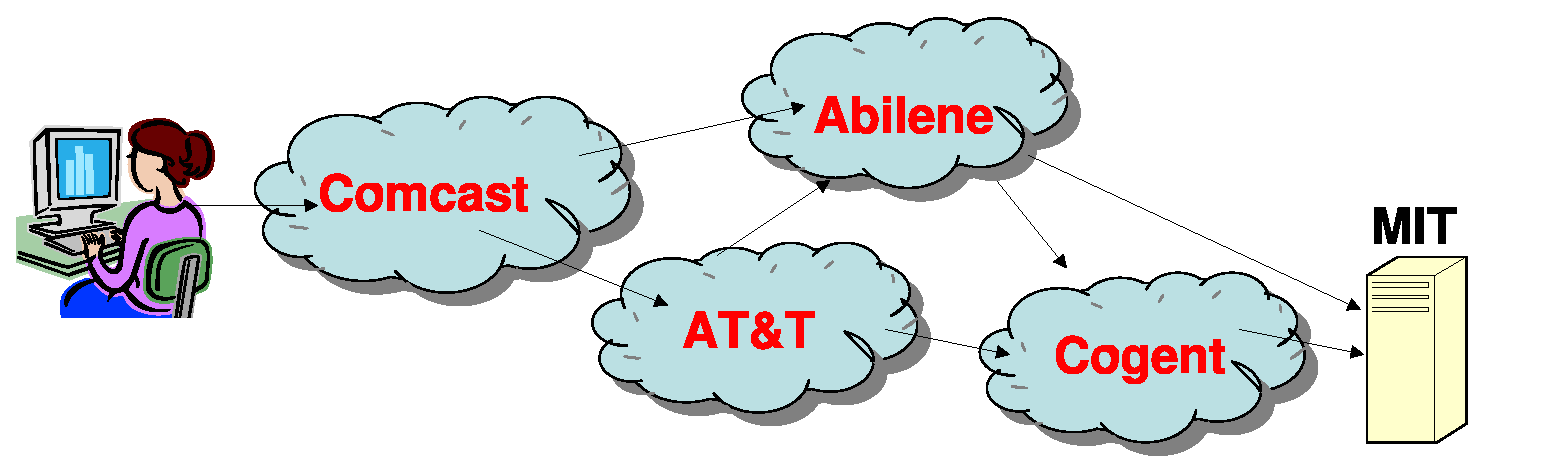
\epsfig{file=figures/overview.eps, width=\linewidth}
\caption[Overview of the Internet's structure]{A typical Internet path may traverse multiple ``Autonomous Systems''.}
\label{fig:intro:overview}
\end{figure}

\begin{figure}[t]
\centering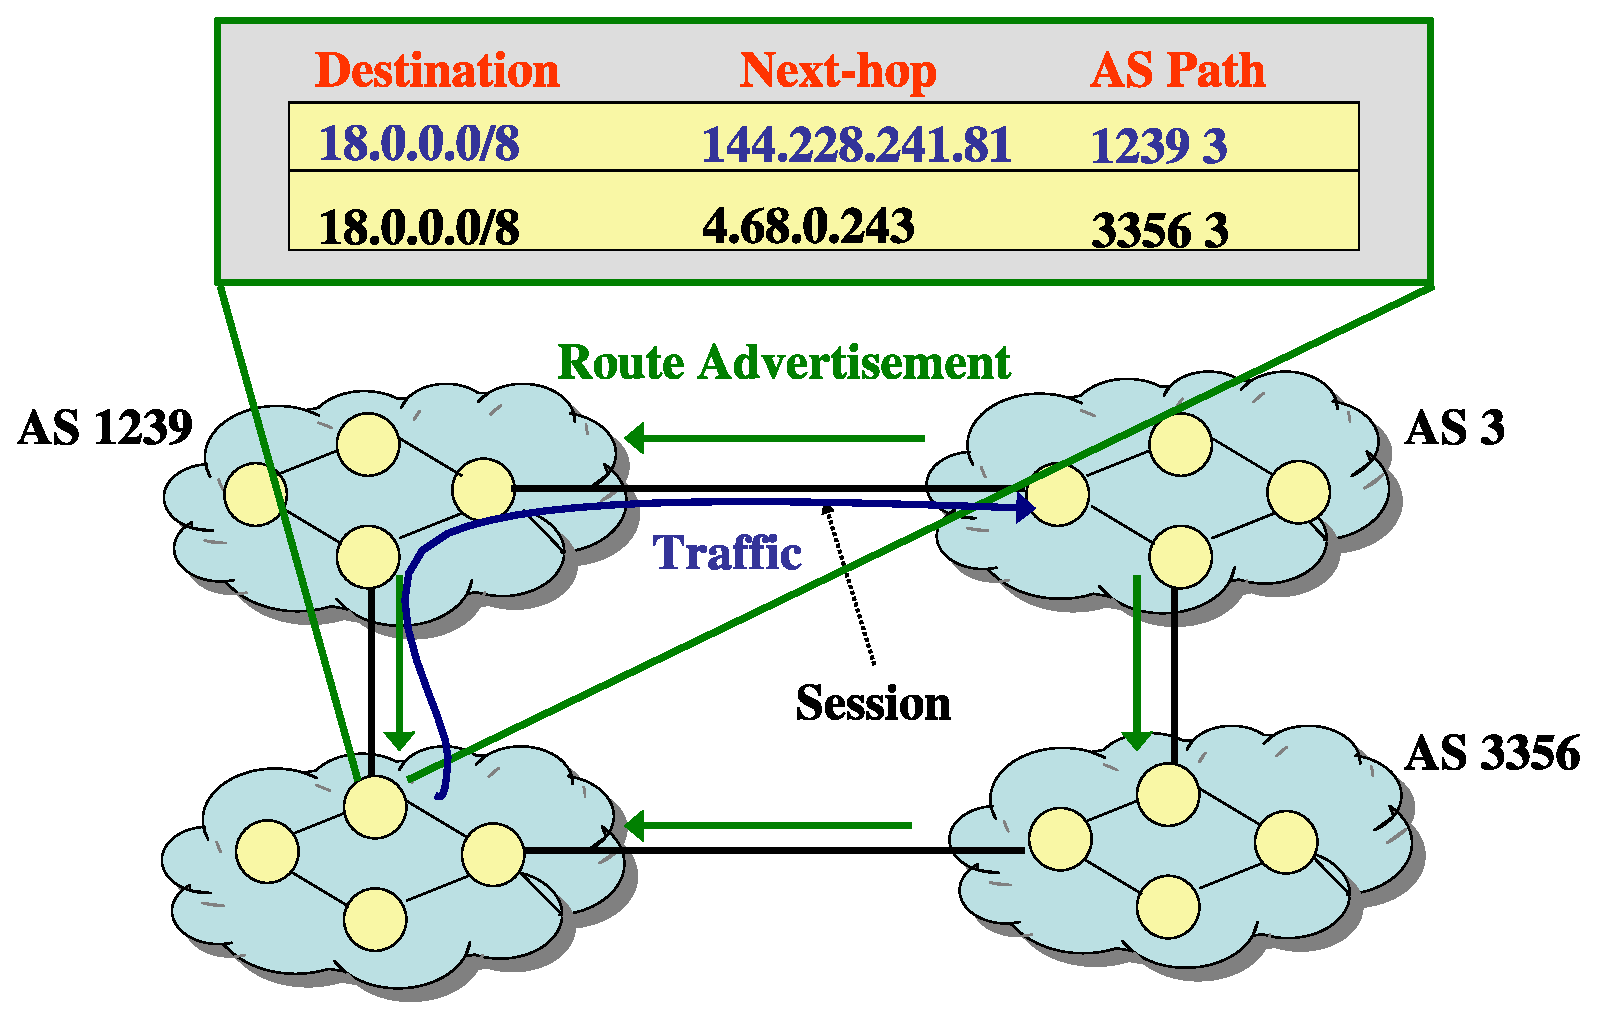
\epsfig{file=figures/rtgtable.eps, width=0.8\linewidth}
\caption[How ASes exchange routing information]{ASes exchange routing
information over BGP {\em sessions} between 
  routers.  A router may learn multiple routes to the destination but
  ultimately selects a {\em single} best route.  Traffic flows in the opposite
  direction of route advertisements.}
\label{fig:intro:rtgtable}
\end{figure}



Although it is common to think of ``the Internet'' as a single, monolithic
network, it is actually composed of tens of thousands of independently
operated networks, commonly called {\em Autonomous Systems} (ASes).
Figure~\ref{fig:intro:overview} shows an example of how traffic from a cable
modem user may traverse multiple ASes en route to machines at MIT.
Internet traffic is forwarded from source to destination through a
sequence of {\em routers} in one or more ASes.  

Each one of these ASes typically has independent (and often
conflicting) economic and performance goals, yet these ASes must cooperate by
exchanging routing information to achieve global connectivity (\eg, to
allow a home user who buys service from his cable modem provider to
communicate with hosts that purchase connectivity from other ASes).
The current routing protocol on the Internet is the Border Gateway
Protocol (BGP)~\cite{rfc1771}.  As shown in
Figure~\ref{fig:intro:rtgtable}, ASes achieve global reachability by
establishing BGP sessions between neighboring ``border'' routers.  Each
AS has may have anywhere from a single router to hundreds of routers. 
%
Each of these routers maintains a {\em routing table}, which contains
one or more routes for each destination.  Each router
selects a single best route to each destination.  Routing on the Internet
is {\em destination-based}; that is, a router selects the next hop (\ie,
router) for which to forward traffic solely based on the destination IP
address of each packet.  The destination for a route is represented in
terms of an IP {\em prefix}, which specifies a group of IP addresses
that share a common number of bits.


\begin{figure*}[tb!]
\begin{center}
\begin{small}
\begin{minipage}{5in}
\begin{verbatim}
   Network          Next Hop            Path
*> 18.0.0.0/8       144.228.241.81      1239 3 
*  18.0.0.0/8       12.0.1.63           7018 3356 3 
\end{verbatim}
\end{minipage}
\end{small}
\end{center}
\caption[Example BGP routing table entry]{BGP routing table entry for
prefix 18.0.0.0/8 as 
  it might appear on a router.  Each BGP route has attributes in
  addition to the next hop IP address and AS path, which we will discuss
  later.}
\label{fig:bgpex}
\end{figure*}


Figure~\ref{fig:bgpex} shows example routing table entries for the set
of destinations represented by the IP prefix {\tt 18.0.0.0/8}, which
represents the $2^{24}$ IP addresses that share the first 24 bits, {\tt
18.*}.  Although each router may learn multiple candidate routes
to a prefix, (\ie, the routing table shown in Figure~\ref{fig:bgpex} has
two possible routes for the same destination), each router ultimately
selects a {\em single} best route for each prefix (in the routing table,
the route that the router ultimately selects is indicated by the ``{\tt
>}''.  The {\em next hop} attribute is the IP address that the router
must forward traffic towards to send traffic along this route.  The
router may learn how to reach this next hop IP address in one of several
ways: a ``static'' route may be hardcoded, the router might learn a
route via a routing protocol that is run inside the AS (\eg, OSPF),
and so forth.  The {\em path} attribute refers to the AS path: the
sequence of ASes that the route advertisement traversed en route to this
router.  
%``Metric'' and ``LocPrf'' refer to the Multiple Exit
%Discriminator (MED) and Local Preference attributes, respectively; an
%operator can manipulate these two attributes to control which route a
%router ultimately selects, given multiple options.  
A BGP route has several additional route attributes that are not
pictured; we will describe
these additional attributes in more detail in Section~\ref{sec:propagation}.

Internet routing requires neighboring ASes to exchange routing
information, but it also requires each of these ASes to run an internal
routing protocol (``Interior Gateway Protocol'', or {\em IGP}) to
establish reachability information about destinations within the same
AS.  For example, in the routing table excerpt shown in
Figure~\ref{fig:bgpex}, the router knows that to forward traffic to any
destination in {\tt 18.*}, it must send the traffic towards the next hop
{\tt 144.228.241.81}.  For ``border'' routers, this next hop is typically
the address of an interface of the router in a neighboring autonomous
system and is an immediate next hop.  Routers within an AS, however,
must use the IGP to discover the outgoing
interface over which to send traffic towards this next hop, which may be
multiple hops away.  This dissertation focuses on BGP but does
not address the operation of internal routing protocols.  Other
work provides more detailed treatment of IGPs~\cite{Feldmann2001,
Shaikh2002, Shaikh2004}.


\section{Configuration: The Achilles' Heel of Internet Routing}
\label{sec:intro:config}

Analyzing the behavior of any routing protocol is inherently difficult,
but Internet routing presents a unique set of challenges because it must
be highly configurable to support the complex economic and performance
goals that each independently operated network is attempting to satisfy.
The standards document for BGP~\cite{rfc1771} specifies the message
format but intentionally leaves unspecified many details, including the
criteria for 
selecting the route to a destination given multiple alternatives.
Instead, these details are left to its {\em configuration}.  In this
section, we 
explain how configuration affects routing protocol behavior; we then
present some examples that demonstrate how configuration mistakes can
induce catastrophic routing failures.

\subsection{How Configuration Affects Routing Protocol Behavior}
\label{ssec:intro:config}

Internet routing configuration provides a network operator remarkable
latitude in controlling how the protocol behaves.  In particular,
Internet routing configuration allows an operator to control the routing
protocol in the following ways:

\begin{itemize}
\item {\bf Which ASes to carry traffic for.}  Depending on the
  business relationships that an AS has established with other
  ASes, it may arrange to carry traffic to a destination for some of
  those ASes but not others~\cite{Gao2001a}.  Routing configuration
  controls which routes an AS advertises to each of its neighbors,
  implicitly controlling which neighbors can send traffic over the
  AS en route to a destination.

\item {\bf How traffic enters and leaves the AS.} An AS
  typically has multiple links over which it can send traffic to a
  destination: some of these links are internal (\ie,
  they are between two routers in the same AS) and others are
  external (\ie, they are between routers in neighboring ASes).
  Changes in traffic demands may cause any of these links to become
  congested.  In response, a network operator may change the routing
  configuration to shift portions of the traffic load to a different set
  of links~\cite{Feamster2002b}. 

\item {\bf How routers within an AS learn routes to external
  destinations.}  Each independently operated network comprises tens to
  hundreds of routers.  Ultimately, every router in the AS must
  learn the routes to external destinations, but, initially, only the
  AS's ``border'' routers learn these routes.  Routing
  configuration controls how the routes propagate from an AS's
  border routers to the rest of the routers in the AS.
\end{itemize}


Changing traffic demands and business relationships, planned
maintenance, and equipment failures may all change traffic patterns
through the AS, but routing protocols do not automatically adapt to
these changing conditions.
As a
result, network operators must constantly tune the behavior of the
routing protocols in their ASes to control how traffic flows through
them.  

\subsection{Problem: Configuration Mistakes Cause Routing Failures}
\label{sec:intro:problem}

The cost of Internet routing's
configurability is a high degree of complexity.  The unfortunate
consequence of this complexity is that the potential for incorrect
behavior is enormous.

The consequences of incorrect behavior can be staggering.  The past few
years alone have seen several high-profile examples of Internet routing
configuration problems:

\begin{itemize}
\item In
1997, a small ISP in Florida configured its routing in a way that caused
all of the Internet's traffic to be routed through it~\cite{www-as7007}.
\item In 2001, Microsoft brought down its Web servers with a routing
misconfiguration; it took nearly a day to diagnose the
problem~\cite{www-microsoft-outage}.  
\item In 2002, Worldcom took down more
than 20\% of its nationwide ``backbone'' in the United States with a
routing configuration problem~\cite{www-worldcom-outage}.  
\item In 2004, Level3 incurred a widespread outage due to a router
configuration problem~\cite{www-l3-outage}.
\item In 2005, an ISP in Bolivia caused a major outage when it announced
the IP prefix for AT\&T's United States backbone
network (\ie, {\tt 12.0.0.0/8}).~\cite{nanog-att}. 
\end{itemize}
Major news outlets report only the most catastrophic routing failures;
in fact, mistakes in routing configuration are continually causing
reasonably serious routing failures.  In the introduction to
Chapter~\ref{chap:rcc}, we 
present the results of our informal study of the mailing list archives
of the North American Network Operators Group (NANOG)~\cite{nanog-list}.
In this study, we 
find that upwards of two-thirds of the routing failures reported on this
mailing list can be attributed to problems with routing configuration.
Network operators are continually misconfiguring routing protocols in
ways that cause such problems as loops, ``blackholes'' (where a router
simply drops traffic en route to some destination because it does not
have a route for it), routing instability, and so forth.  

%%%%%%%%%%%%%%%%%%%%%%%%%%%%%%%%%%%%%%%%%%%%%%%%%%%%%%%%%%%%

\section{Challenges}\label{sec:challenges}

While guaranteeing correct and predictable behavior poses challenges for
any routing protocol, Internet routing presents several unique
challenges.  First, Internet routing has more configurable facets
than traditional routing protocols, many
of which can be misconfigured or otherwise cause the routing protocol to
behave unpredictably.  In order to analyze the correctness of the
routing protocol, we must first define a specification for correct
behavior.  Second, the sheer size of the distributed
router configuration, as well as the fact that the configurations have
dependencies across routers, can give rise to erroneous or unpredictable
behavior.  Third, because each network operator configures his AS
independently of others, the policies defined in one AS may conflict
with those in neighboring ASes.

\subsection{Defining a Correctness Specification}

As described in Section~\ref{ssec:intro:config}, Internet routing
configuration affords a network operator much flexibility in defining
how the protocol operates.  The Cisco configuration language has more
than 1,000 different commands, and a network of 500 routers may have
upwards of one million lines of configuration distributed across the
AS~\cite{www-cisco-ios-master}.  Given the many ways in which an
operator can affect protocol behavior, determining the correctness of
the configuration is a daunting task without a high-level specification
for ``correct'' behavior.  Developing such a specification involves
distilling the high-level properties that the protocol should satisfy
from the protocol's mechanistic detail.

Defining a correctness specification for Internet routing is complicated
by the fact that the protocol's correctness is in part 
based on whether it achieves a network operator's economic
and performance goals.  Unfortunately, these high-level policies are
encoded in terms of mechanistic configuration commands distributed
across hundreds of routers---that is, the specification of the {\em
intended} behavior doesn't even exist in the first place, which makes it
difficult to determine whether the routing configuration indeed induces
the intended behavior.

One motivation for developing a correctness specification for Internet
routing is that the protocol not only ``does the right thing'' when it
satisfies the specification, but a routing protocol that satisfies the
specification is also more predictable.  For example, network operators
often would like to predict the effects of a configuration change on the
behavior of the routing protocol without testing that change on a live
network or running a complex simulator.  Predicting how the protocol
will behave first requires making assumptions about its behavior to
simplify route prediction, but precisely determining the constraints that
are required to simplify route prediction for such a complex protocol is
challenging.

\subsection{Analyzing Complex Configuration}

%% Configuring a network's routing boils down to independently configuring
%% the routers within a network.  Each network contains as many as several
%% hundred routers; each of these routers may have tens of thousands of
%% lines of configuration.  Although an operator configures each of these
%% routers separately, the configuration typically has dependencies across
%% multiple routers in the network.  Furthermore, a network may contain
%% routers from different vendors, each of which have a different
%% configuration language.  The configuration of these routers collectively
%% dictates the behavior of the network. In this sense, configuring a
%% network of routers is not unlike writing a large distributed program in
%% several different flavors of assembly language.  Given this complexity,
%% it is not surprising that network operators make mistakes in configuring
%% routers.

In designing tools that can help network operators reason
about the correctness of Internet routing, we must also design ways
to manage routing configuration's staggering complexity.  First, we must
represent this 
distributed router configuration in a format that is easy to analyze.
Second, we must tackle the engineering problem of parsing the various
routing configuration languages from different vendors and translating
the configurations into this format.

Determining how a configuration change will affect routing is difficult
in practice.  Not only do ASes contain a large number of routers, but
the route that each router ultimately selects for each destination
depends on many factors, including the routes that the AS's ``border''
routers learn from neighboring ASes, the routing topology within the AS
(\ie, both the internal topology, and the internal BGP topology that
controls how routes are disseminated within the AS).  As we discuss in
more detail in Chapter~\ref{chap:sandbox}, various complicating
protocol artifacts prevent informally reasoning about the route that each
router selects.  Thus, network operators need tools and
systematic techniques to assist them in predicting how a particular
routing configuration will affect the flow of traffic through the AS.


\subsection{Providing Global Guarantees with Only Local Information}

While end-to-end connectivity between Internet hosts fundamentally
depends on the {\em global} behavior of the routing system, no single party
has a global view of the Internet routing system. A network operator may
configure the protocol in a way that interacts in unexpected ways with
the configurations in other ASes.  For example, the interactions of
routing policies in neighboring ASes can cause the routing protocol to
oscillate.

One goal of our work is to explore how we can achieve assurances about
the global behavior of the Internet routing system, while still
preserving the {\em autonomy} of each AS.  That is, each network operator
should retain the ability to independently configure his own AS,
but should also be able to gain some assurances about the global behavior of
the routing system, assuming every AS abides by a similar set of
rules.  


%%%%%%%%%%%%%%%%%%%%%%%%%%%%%%%%%%%%%%%%%%%%%%%%%%%%%%%%%%%%


\section{The Role of Proactive, Static Configuration
Analysis}\label{sec:proactive}  

\begin{figure}[t]
\centering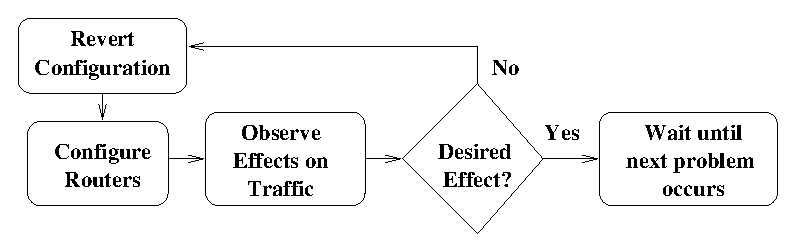
\epsfig{file=figures/workflow.eps, width=0.7\linewidth}
\caption[The state-of-the-art in network configuration management]{The state-of-the-art in network configuration management: {\em
reactive}, ``stimulus-response'' mode of operation.}
\label{fig:intro:workflow}
\end{figure}

Prior to our work, the state-of-the-art in managing Internet routing
protocols was {\em reactive}: the primary way for network operators to
determine the effects of a particular routing configuration (\ie, what
effects that configuration will have on the flow of traffic, or whether
the configuration is even correct in the first place) was to deploy that
configuration on a live network, observe the resulting behavior, and
revert the configuration to a previous version in the event that the
configuration did not produce the desired effects (see
Figure~\ref{fig:intro:workflow}).  This mode of operation has two
shortcomings: First, testing configuration on a live network can cause
unnecessary downtime or poor network performance (and, hence, angry
customers!).  Second, the undesirable effects that result from a
particular configuration may not be immediately apparent when the
configuration is deployed; a failure may only be triggered by the
presence or absence of certain routes.

This dissertation posits that {\em proactive} techniques for analyzing
routing configuration can both prevent a large class of routing failures
and help operators predict and analyze routing protocol behavior.
Changing the workflow from Figure~\ref{fig:intro:workflow} to include a
step that proactively detects problems with routing configuration is
critical for improving the correctness and predictability of Internet
routing.  A remarkable result of our work is that proactive analysis
techniques (\ie, those that analyze the static routing configuration
offline, before it is deployed on a live network) are useful in
detecting configuration faults and efficiently and accurately predicting
the routing protocol's behavior.  In particular, proactive analysis
techniques provide the following benefits over the status quo:

\begin{enumerate}
\itemsep=-1pt
\item {\bf Offline.}  A reactive mode of configuration is time consuming
and can lead to unnecessary performance degradation.  The complexity of
Internet routing makes it essentially impossible to compute
back-of-the-envelope estimates of the effects of configuration changes.
Proactive techniques for determining the correctness and the effects of
Internet routing configuration can help network operators evaluate the
effects of a routing configuration before it is deployed on a live
network.

\item {\bf Accurate.}  Network simulators (\eg,
ns~\cite{www-ns-bgp}, SSFNet~\cite{www-ssfnet}) help operators
understand dynamic routing protocol behavior, but simulation models
network behavior in terms of its protocol dynamics over some certain
period of time.  The {\em outcome} of the simulator will ultimately be
the same as that predicted by static techniques, and the dynamics (which
are nondeterministic) may not necessarily correspond to those in the
actual network anyhow.  Existing simulators do not capture all of the
relevant protocol interactions that may affect correctness, nor do they
explain {\em why} a particular configuration is incorrect.  Because
incorrect behavior sometimes depends on a particular sequence of route
advertisements or may be nondeterministic, correct behavior in a
simulator cannot guarantee correct behavior on a live network.  In this
dissertation, we show that techniques based on direct analysis of static
configuration files can test for necessary or sufficient correctness
conditions and predict the outcome of the routing protocol without
having to simulate the protocol dynamics.

%% While simulators can
%% prove useful, they are often unnecessarily complex: simulators can help
%% an operator study the {\em dynamics} of the network, but operators
%% typically do not care about such dynamics; rather they need to quickly
%% evaluate the {\em outcome} of the route selection process.


\item {\bf Efficient.}  Because network operators cannot use ``back of the
envelope'' calculations to determine what a particular routing
configuration will do, they must often experiment with many
possibilities before arriving at an acceptable solution.  As we will
show in Chapters~\ref{chap:rcc} and~\ref{chap:sandbox}, static analysis
techniques can assist network operators in efficiently determining the
correctness and effects of incremental changes to a routing
configuration.


\end{enumerate}

%% This dissertation presents techniques for determining both the
%% correctness and the outcome of this computation (1)~efficiently, (2)~in
%% a way that facilitates evaluating incremental changes, and (3)~without
%% having to observe the protocol's behavior on a live network.

Analyzing the static router configurations of a single AS proves
surprisingly effective at improving the correctness and predictability
of Internet routing.  An important open question that is {\em not}
addressed in this dissertation involves
exploring the classes of faults that {\em cannot} be detected with
static analysis alone and how analysis of routing {\em dynamics} might
complement static configuration analysis for fault detection and diagnosis.

%% this dissertation also recognizes
%% the limitations of static analysis.  We explore how dynamic analysis of
%% routing protocol messages can complement static configuration analysis,
%% and even changes to the routing protocol and architecture itself.



%%%%%%%%%%%%%%%%%%%%%%%%%%%%%%%%%%%%%%%%%%%%%%%%%%%%%%%%%%%%

\section{Contributions}\label{sec:contributions} 

We now briefly overview the major contributions of this dissertation
before describing each in more detail.  A central contribution of this
dissertation is a formal correctness specification for Internet routing.
We use this specification to derive tests for configuration faults and
as the groundwork for efficient offline analysis of Internet routing.
Using this specification as a guide, we present the design and
implementation of two systems that use proactive configuration analysis
techniques to improve the correctness and predictability of Internet
routing.  The first, \rcc (``router configuration checker''), detects
faults in routing configuration. \rcc helps network operators eradicate
configuration faults before they cause catastrophic routing failures on
a running network. The second, the {\em routing sandbox}, efficiently computes
the routes that each router within a single AS ultimately select, using
only a static snapshot of the routing configuration and network state.
%The
%BGP sandbox allows an operator to experiment with configuration changes
%offline and determine whether a possible configuration change would have
%the desired effect, before deploying the change on a live network.

Because Internet routing inherently involves interaction between
multiple independently operated, competing ASes, some aspects of the
correctness 
specification are difficult to verify by only looking at the
configuration of a single AS in isolation.  In particular, it turns out
to be difficult to determine whether the routing protocol will converge
to a stable route assignment (a property defined as {\em safety} in
previous work~\cite{Varadhan1996}).  Traditional routing protocols
typically satisfy safety, but BGP's {\em policy-based} nature means that
the policies of neighboring ASes can interact to create oscillations.
This dissertation provides the first necessary conditions for
guaranteeing the stability of a policy-based routing protocol.  The rest
of this section discusses these contributions in more detail.

%% While analyzing the static router configurations of a single AS
%% proves surprisingly effective at improving the correctness and
%% predictability of Internet routing, this dissertation also recognizes
%% the limitations of static analysis.  We explore how dynamic analysis of
%% routing protocol messages can complement static configuration analysis,
%% and even changes to the routing protocol and architecture itself.
%% Specifically, we present the design of the Routing Control Platform
%% (RCP), a routing system that separates the route selection logic from
%% the routers themselves and can explicitly guarantee many aspects of the
%% correctness specification.


%This dissertation also makes practical contributions in the areas
%of network management and Internet routing design.  While the
%contributions to network management may prove more immediately
%applicable, we believe that the work more relevant to routing design
%will ultimately make Internet routing intrinsically more robust and
%predictable.  In other words, while network management tools are crucial
%to network operation, our ultimate goal should be to {\em design the
%protocol for manageability}.  Our contributions to routing protocol
%design are a step in the right direction towards this goal.

\subsection{A Correctness Specification for Internet Routing}

We define three high-level properties that a routing
protocol should satisfy. Essentially, all three aspects of this
correctness specification
reflect the following underlying principle: {\em a routing protocol
should propagate 
information that accurately reflects the properties of the underlying
network topology}.  The three properties are as follows:

\begin{itemize}
\item {\bf Route validity.}  If an endpoint learns a route to a
  destination, then that route should correspond to some path.  An
  example of a route validity violation would be a persistent forwarding
  loop: a router learns a route to some destination (\ie, a destination,
  and the next-hop IP address to which traffic should be sent for that
  route), but when it actually attempts to send traffic along that
  route, it is caught in a forwarding loop and never reaches
  the destination.

\item {\bf Path visibility.}  If there exists a sequence of IP-level
  hops (\ie, a {\em path}) from an endpoint to a destination, then
  that endpoint should learn at least one route to that destination.  An
  example of a path visibility violation would be a case where all
  routers inside a fully-connected AS did not learn a route to the
  destination when at least one of those routers learned the route.  

\item {\bf Safety.}  This property requires that the
  routing protocol ultimately assigns a route to each node in the
  Internet graph 
  such that no node has a more preferred available route to the
  destination that it would rather use.  Safety is important not only
  because a routing protocol that persistently oscillates can cause lost
  and reordered packets, but also because it is incredibly difficult to
  diagnose problems when the routing protocol is changing independently
  of the underlying topology.  A violation of safety would be an
  oscillation caused by conflicting policies from different ASes (rather
  than due to topological changes), as described in previous
  work~\cite{Griffin2002c, Varadhan1996}.
\end{itemize}

Chapter~\ref{chap:rlogic} formalizes each of these
properties, as well as well as other concepts (\eg, path,
route, etc.).  Path visibility and route validity are violated primarily
because of configuration complexity, and safety is violated because the
configurations of one AS may interact in unexpected ways with
configurations of other ASes.

Although this dissertation applies this correctness specification to
Internet routing, these properties should prove valuable for analyzing
any routing protocol.  Applying these properties to routing in other
areas (\eg, wireless or sensor networks) is beyond the scope of our
work, but is ripe for exploration.

\subsection{Systems for Proactive Fault Detection and Route Prediction}

This dissertation recognizes a critical missing piece in the {\em
workflow} of configuring today's networks: the step at which network
operators evaluate the effects of a routing configuration before
deploying and running it on a live network.


\begin{figure}[t]
\centering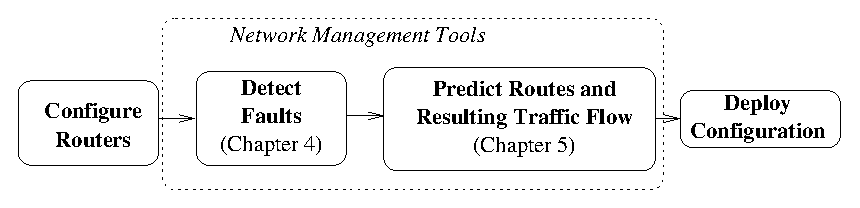
\epsfig{file=figures/workflow2.eps, width=0.75\linewidth}
\caption[This dissertation's contributions in fault detection and
route prediction.]{This dissertation develops two tools for fault detection
  and route prediction.  These tools should be used to analyze the
  behavior of routing configuration before it is deployed on a live
  network.}
\label{fig:intro:workflow2}
\end{figure}


\begin{figure}[t]
\centering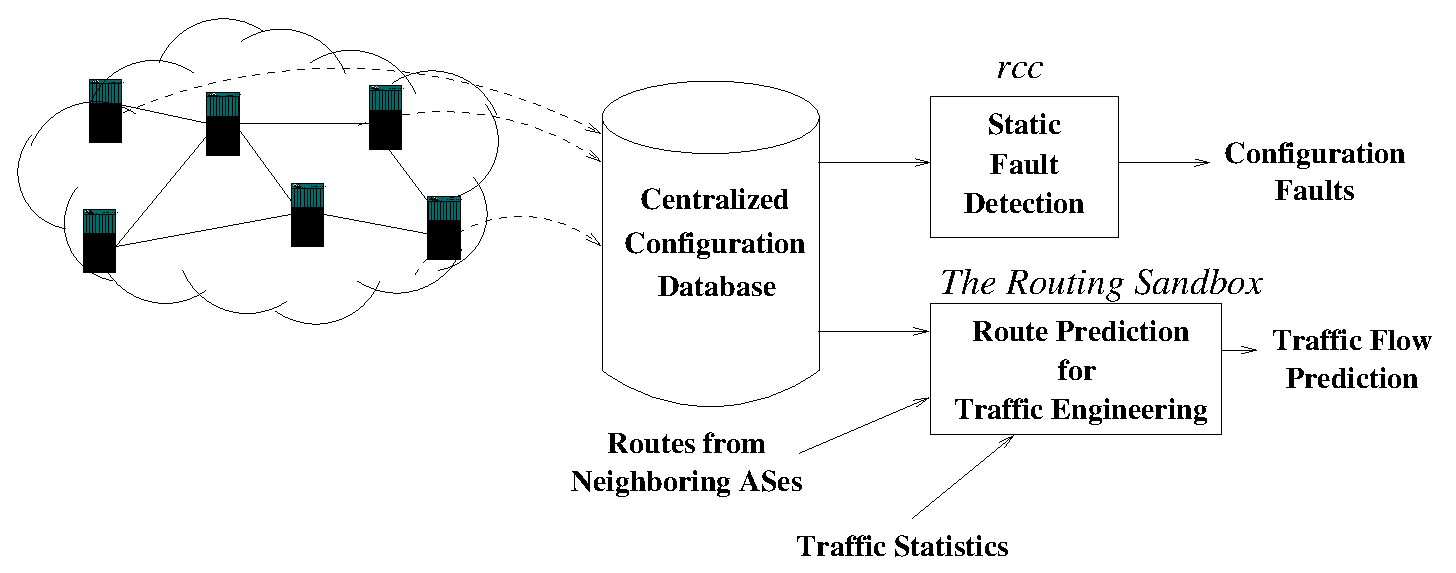
\epsfig{file=figures/process.eps, width=0.9\linewidth}
\caption[Workflow for fault detection and route prediction
  tasks.]{Workflow for fault detection and route prediction tasks 
  described in this dissertation. Both fault detection and route
  prediction tasks rely on {\em offline} analysis of the distributed 
  router configurations, which are first collected into a centralized
  database.}
\label{fig:intro:process}
\end{figure}


This dissertation presents two complementary systems that advance the
state-of-the art in fault detection and traffic engineering,
respectively.  Figure~\ref{fig:intro:workflow2} shows how these two
systems change the workflow of configuring routers.  Both of these new
systems analyze the {\em static} router configuration files.  We first
describe \rccns, a fault detection system for router configurations.  We
then describe the {\em routing sandbox}, a tool that predicts how traffic
will flow through an AS, given only a static snapshot of the router
configurations.  Together, these contributions assist a network operator
in detecting faulty routing configurations and determine the effects of
a configuration on traffic flow.

Because the techniques we present predict the behavior of the routing
protocol before it even runs, the techniques we present directly analyze
of the static configuration files.  Figure~\ref{fig:intro:process}
illustrates this process.  The configurations from the routers within an
AS are first collected from the routers and stored in a central
database.  Fault detection is performed by executing queries directly
against this repository (Chapter~\ref{chap:rcc} provides more details).
Route prediction for traffic engineering (Chapter~\ref{chap:sandbox}) is
performed in a similar fashion, but also requires additional inputs:
computing the routes that each router selects requires knowing which
routes each router learns from neighboring ASes in the first place.
Once the route that each router ultimately selects is computed, an
operator could use traffic statistics to determine the utilization on
each link in the network, but this dissertation does not address this
problem.

\subsubsection{\rccns: Proactive fault detection for Internet routing
configuration}

Chapter~\ref{chap:rcc} presents the design and implementation of \rccns,
the ``router configuration checker'', a tool that uses static 
configuration analysis to detect faults in the routing configurations
within a single AS.  We designed \rcc starting with the correctness
specification as a guide and determining the constraints on the 
aspects of configuration (described in more detail in
Section~\ref{sec:semantics}) that must hold to guarantee that the
higher level correctness properties are satisfied.  \rcc analyzes the
set of router configurations from a single AS and determines whether
they could induce violations of the correctness specification.  

{\em rcc} has been downloaded by over seventy network operators, and we
have personally used {\em rcc} to study faults in the
routing configurations of $17$ real-world ASes.
Chapter~\ref{chap:sandbox} presents algorithms and a tool that helps
network operators predict how a particular routing configuration will
affect the flow of traffic through the AS.  In conjunction with
{\em rcc}, this tool allows a network operator to answer critical
questions about routing configuration (\ie, whether the configuration
will cause catastrophic problems, and how it will affect the flow of
traffic through the AS) {\em before} the configuration is actually
deployed on a live network.

Our work on \rcc demonstrates that static configuration analysis can
detect a significant number of configuration faults that could cause the
routing protocol to violate correctness. Surprisingly, \rcc also
discovered many such faults in {\em deployed} routing configurations,
even those from large, well-known Internet service providers.  \rcc even
found configuration faults in ASes that use ``automated''
configuration techniques: of course, automated configuration systems
will have difficulty generating correct configuration if they do not
receive correct input in the first place.  Many of the
configuration faults that \rcc detects in practice suggest that
configuring a network 
of routers without introducing inconsistencies across router
configurations is surprisingly difficult.

%% Although \rcc uses only static analysis of routing configuration to
%% detect faults, some routing faults are best detected using analysis of
%% routing protocol dynamics in concert static configuration analysis may
%% also prove useful for detecting routing faults.  In
%% Chapter~\ref{chap:concl}, we speculate on scenarios where dynamic
%% analysis may prove useful.

\subsubsection{The Routing Sandbox: Proactive route prediction for
network engineering}

Chapter~\ref{chap:sandbox} describes algorithms that compute the effects
of a configuration change offline, given only a static snapshot of the
routing configurations and the available routes.  These algorithms can
then be combined with information about traffic demands to help network
operators determine how a particular routing configuration will affect
the flow of traffic through the AS.  Rather than simulating complex
protocol dynamics to determine the effects of configuration on route
selection, we model the {\em outcome} of BGP's route selection process.
{\em We exploit the properties of the correctness specification to
simplify this process:} assuming that \rcc has already verified that the
configuration satisfies route validity, path visibility, and safety
makes it possible to model AS-wide route selection without simulating
the dynamics of the routing protocols.

Route prediction becomes increasingly difficult in ASes that enable two
protocol ``features'': the Multiple Exit Discriminator (MED) attribute
and route reflection, which are described in
Sections~\ref{sec:propagation} and~\ref{sec:dissemination}, respectively.
We design algorithms for predicting BGP 
route selection for ASes that have any combination of these two features
enabled.  We also perform a running-time analysis of each of these
algorithms, which provides insight into how each of these features adds
complexity to Internet routing.

We have implemented these algorithms in a tool called the {\em routing
sandbox} that allows a network operator to {\em quickly} evaluate the
effects of incremental configuration changes.  This tool exploits
several unique aspects of the system inputs to optimize the computation
of routes for all destinations for every router in the AS.  We envision
that the routing sandbox could be used as an ``inner loop'' to other
tools that iteratively search through a large parameter space to find
optimal settings~\cite{Ye2003}.

\subsection{Conditions for Safety of the Global Routing System}



Configuration allows an operator to control both the route that each
router selects to a destination (\ie, {\em ranking}) and which routes
each router readvertises to neighboring routers (\ie, {\em filtering}).
One way to guarantee safety is to restrict some aspects of the
configuration's flexibility.  In Chapter~\ref{chap:policy}, we derive
necessary and sufficient conditions on the policies of each AS that
guarantee safety
if each AS independently follows these constraints.  Specifically, we
explore how each AS 
must restrict rankings to guarantee that the global routing system
satisfies safety, assuming that no AS wants to share its rankings with
any other AS, and no AS's rankings should be constrained by the rankings
of another AS (that is, each AS should retain {\em autonomy}).

We show that any protocol that does not restrict the business
arrangements of how ASes exchange routes with one another must impose
strong restrictions on how ASes are allowed to express preferences over
candidate routes for a destination.
%
Initially, this finding may sound rather grim, because shortest paths
routing may not provide network operators sufficient flexibility to
achieve their economic and performance goals.  On the contrary, the
results we present in this dissertation should be viewed as a first cut
towards designing routing protocols that are guaranteed to satisfy
safety, regardless of how they are configured.  Today, network operators
have no way to reason about the stability of the routing protocol, so
they are left to {\em ad hoc} methods for determining whether routing
updates correspond to unintended interactions.  A routing protocol that
conforms to the guidelines we outline in Chapter~\ref{chap:policy}
guarantees that changes in the routing protocol always reflect changes
in the underlying topology, thereby facilitating troubleshooting.
Furthermore, designing a protocol that is guaranteed to satisfy safety
on a fast timescale allows conflicts of business policy to be resolved
{\em outside} the protocol, rather than being reflected as oscillations
within the protocol itself.


\section{Lessons Learned}\label{sec:lessons}

This dissertation provides the following important lessons that can aid
the networking community as it considers proposals for evolving the
Internet routing infrastructure.

\subsection{Static configuration analysis detects many faults}

\rcc detected configuration faults in the routing configurations of all 17
ASes we analyzed and more than a thousand faults overall.  It may
seem surprising that \rcc was able to detect configuration faults in
{\em deployed} routing configurations.  In fact, this finding
demonstrates that there are many potentially catastrophic configuration
faults that do not immediately cause routing failures when they are
deployed.

The fact that static analysis can find important configuration faults
without overwhelming network operators with a vast quantity of false
positives is also somewhat remarkable.  \rcc does {\em not} operate with
a specification of the routing protocol's intended behavior.  Rather, it
operates solely on the routing configurations that {\em implement} an
operator's intent with low-level mechanisms.  Ideally, \rcc would check
the router configurations against a high-level specification of intended
behavior.  It is noteworthy that \rcc can provide a useful tool to
network operators in the absence of such a specification.

Configuration languages may ultimately evolve to make certain types of
configuration faults less likely, but static configuration analysis will
remain a crucial step in the workflow of network operations.  We believe
that the more mechanistic aspects of routing configuration will
ultimately be supplanted with high-level policy specification.  For
example, preventing routes that were learned from one neighboring
AS from being advertised to another today requires configuring
low-level, mechanistic operations on every router that exchanges routes
with either of those ASes.  Such a simple policy would better be
expressed in a specification language and ``compiled'' to the statements
that implement the mechanisms on the routers themselves.  However,
because Internet routing must always afford a network operator
flexibility in controlling the behavior of the protocol, static
configuration analysis will be invaluable for detecting faults and
evaluating routing protocol behavior, {\em
regardless of the configuration language}.  

\subsection{Distributed routing configuration leads to errors}

Our study of configuration faults in Chapter~\ref{chap:rcc}
(Section~\ref{sec:evaluation}) demonstrates
that most configuration faults result from the fact that routing
protocol configuration is {\em distributed} across the routers in the
AS.  This approach naturally causes operators to make mistakes because
it is more natural to think of the AS {\em as a whole} as implementing
some certain task (\eg, controlling traffic flow, implementing
contractual arrangements, etc.) rather than reasoning about what each
router must do to implement such a task.  A better approach may be to
allow operators to configure the AS as a monolithic entity from a
single location.

Of course, a crucial open research challenge upon which this goal
depends is what that centralized language should look like, and how the
routers themselves should implement the directives in that language.
Recent work in constraint satisfaction for network configuration
presents a possible starting point for a centralized configuration
language that satisfies high-level specification~\cite{Narain2004}.

A logically centralized routing infrastructure could act as
a catalyst for such a centralized configuration language.  For example,
a network operator could configure the AS from the RCP, which could
either (1)~compile this high-level specification into low-level router
configurations, and {\em push the configuration} to the individual
routers or (2)~select the routes on behalf of each router and {\em push
the routes} themselves to the routers.

\subsection{Safety + Autonomy $\Rightarrow$ Tight restrictions on
expressiveness} 

The (strict) conditions we derive in Chapter~\ref{chap:policy} for
guaranteeing safety suggest several possible ways for evolving the
Internet routing infrastructure.  One possibility is to relax the
autonomy requirement, by allowing groups of ASes to share certain
properties about their rankings with one another (although likely not the
rankings themselves).  Recent work has begun exploring this possibility
by recognizing that some ASes may have rankings that are more expressive
as long as others are not and designing ways to guarantee these global
properties without requiring ASes to divulge sensitive information about
rankings~\cite{Machiraju2004}.  One area for future work to determine
the information that must be shared (and with what other ASes it must be
shared) to detect and {\em resolve} safety violations, and, in
general, to study the tradeoffs between safety and the autonomy and
privacy of an ASes rankings.

Another possibility for evolving the Internet routing system is to
restrict expressiveness so that rankings must be consistent with
shortest paths routing, but allow each AS to control the weights on
edges incident to itself.  Such a routing protocol would always
satisfy safety (even assuming ASes are allowed to filter routes
arbitrarily), and any
%but the protocol may converge to a path assignment that a
%network operator does not want, hence causing the operators of each
%AS to repeatedly fiddle with rankings.  If a set of ASes have a
%legitimate policy conflict (\eg, a set of ASes all prefer routes through
%each other, thus creating a cycle of preferences), the protocol would
%then oscillate in accordance with network operators updating their
%rankings.  Such 
policy disputes could then be resolved with a negotiation protocol that
operates independently of the routing protocol, where routing updates
would only reflect actual changes in the network topology.  We explore
this possibility and others in detail in
Chapter~\ref{chap:policy} (Section~\ref{sec:policy:implications}).
 

\subsection{Protocol design should consider correctness and
predictability}\label{sec:mods} 

This dissertation focuses on improving the correctness and
predictability of the current Internet routing system, but a major
lesson from our work is that many of the tools and techniques that we
develop in the coming chapters could have been much simpler had the
protocol been designed with correctness and predictability in mind in
the first place.  

To this end, this dissertation proposes several minor modifications to
the Internet routing protocol that would have simplified the task of
achieving correct and predictable behavior.  These modifications are
minor in the sense that they can be implemented with no modifications to
routers or routing protocol specifications; on the other hand, they are
significant because they eliminate the artifacts that result from the
two most troublesome aspects of BGP: route reflection and the ``multiple
exit discriminator'' (MED) attribute.  In summary, we will see that
these two artifacts are responsible for much of the undesirable behavior
in Internet routing, ranging from persistent oscillation to network
partitions.  
%% In Chapters~\ref{chap:policy} and~\ref{chap:sandbox}, we will see that
%% much of the complexity of predicting the outcome of BGP route selection
%% is caused by route reflection, the MED attribute, and the interaction
%% between these two artifacts.  While MED serves a useful purpose in
%% allowing one AS to express preferences over exit points to its neighbor,
%% it also can create protocol oscillations, because the presence or
%% absence of some route can affect a router's relative preference between
%% two {\em different} routes.  This behavior arises because different
%% neighboring ASes may assign different MED values; as a result, a router
%% can only compare the MED values among routes from the {\em same} AS for
%% that destination, not across all routes for that destination.  In
%% Chapter~\ref{chap:sandbox} (Section~\ref{sec:sandbox:med_disc}), we
%% propose a small modification to BGP configuration that allows the MED
%% attribute to be compared across all routes to a destination (thus
%% eliminating the possibility for MED-induced oscillations) but still
%% preserves the ability for a neighboring AS to express relative
%% preferences over exit points.

One logical conclusion that can be drawn from the work in
this dissertation is that, rather than trying to {\em infer} the
protocol's behavior, the Internet routing system should provide more
direct {\em control} over route selection.
%
This insight is central to the Routing Control Platform (RCP) proposal,
which we describe briefly in Section~\ref{sec:rcp}.  RCP takes as input
the routes that an AS learns from neighboring ASes and the network
configuration, and computes routes on behalf of each router in the AS.
In some sense, RCP can be viewed as the logical extension to the routing
sandbox: RCP takes roughly the same inputs as the sandbox, but rather
than simply computing the routes that each router would select, RCP
actually controls route selection.

%% RCP
%% ensures that the route assignments for each router are based on a
%% complete view of the AS topology, and that routers are selecting paths
%% through the AS in a consistent fashion, thereby preventing forwarding
%% loops, blackholes (\ie, instances where traffic arrives at a router that
%% has no routing table entry for it), etc.  Recent work has demonstrated
%% that RCP can be used to perform route selection on behalf of all of the
%% routers in a large tier-1 ISP~\cite{caesar2004}, but many questions
%% remain.  Chapter~\ref{chap:concl} (Section~\ref{sec:rcp}) presents an
%% initial design of RCP and discusses the various benefits it could
%% provide (as well as open questions).

%\subsection{Eliminating MED while retaining its benefits} 





\section{How to Read This Dissertation}\label{sec:guide}

The problems with today's Internet routing infrastructure suggest one of
two attitudes:

\begin{enumerate}
\item Accept the Internet routing architecture ``as is'' and retrofit
  correctness and predictability by providing tools and techniques that
  make network operations less prone to faults and more predictable.
\item Adapt the routing architecture to make incorrect behavior
  less likely in the first place.
\end{enumerate}

Various parts of this dissertation cater to each of these philosophies.
The former philosophy can have more immediate impact and in fact can
provide ``bottom up'' insight regarding what aspects of the routing
architecture are most problematic.  Chapters~\ref{chap:rcc}
and~\ref{chap:sandbox} adopt this philosophy by providing tools and
algorithms that have helped network operators {\em today}.  \rcc has
been downloaded by over seventy network operators and has successfully
detected faults in the configurations of many large backbone Internet
Service Providers.  Additionally, the faults that \rcc uncovered in our
analysis of 17 real-world ASes, as well as the various aspects of BGP
that contribute complexity to the algorithms in
Chapter~\ref{chap:sandbox}, have helped us identify the aspects of the
routing architecture that beg for improvement.

Chapter~\ref{chap:policy} explores possibilities for improving routing
stability that will most likely require fundamental changes to the
Internet routing architecture because the conditions for stability would
require changing the configuration ``knobs'' that are exposed to network
operators.  The problems examined in this chapter use restrictions on
{\em static} configuration of the routing protocol to guarantee stable
dynamics.  
%% Section~\ref{sec:rcp} moves beyond simple static analysis,
%% proposing a fundamentally new mechanism for disseminating routes within
%% an AS and opening up new possibilities (as well as many unanswered
%% questions) for network management and configuration.

This dissertation caters both to the theoretician and the practitioner.
Chapter~\ref{chap:rlogic} presents a correctness specification for
Internet routing that could appeal to both parties.  Those most interested in
practical applications should focus primarily on Chapters~\ref{chap:rcc}
and~\ref{chap:sandbox}; Chapter~\ref{chap:policy} has fewer immediate
practical applications, but will be of interest to those interested in
fundamental results on routing stability and safety.  At the end of
Chapters~\ref{chap:rcc},~\ref{chap:sandbox}, and~\ref{chap:policy}, we
explore possibilities for 
evolving the Internet infrastructure to make the problems we solve
easier in the future; these sections should also have broad appeal.

%a thorough treatment (and
%hopefully lucid explanation) of Internet routing stability.

\setcounter{chapter}{1}

\section{Background}\label{sec:bg_stability}


\begin{center}
\begin{table}
\begin{tabular}{l|l|p{3.15in}} 
{\bf Year} & {\bf Author} & {\bf Major Results} \\ \hline 
1996 & Varadhan \ea~\cite{Varadhan1996,Varadhan2000} & Observed that
policy-based 
routing protocols may never converge (\ie, they may be ``unsafe''). \\
%
1999 & Griffin \ea~\cite{Griffin2002c,Griffin99} & Showed NP-hardness of
determining safety, and derived sufficient global conditions for
safety. \\ 
%
2001 & Gao and Rexford~\cite{Gao2001a} & Derived restrictions
on routing configuration and topology that guarantee safety, and
observed that these conditions are similar to common practice. \\ 
%
2003 & Sobrinho~\cite{Sobrinho2003} & Developed an algebraic framework
for general path vector, policy-based protocols and derived properties
that the algebra must have to guarantee convergence. \\
%
2003 & Griffin
\ea~\cite{Griffin2003} & Laid out design tradeoffs in policy-based
routing protocols: expressiveness, modularity, etc.\\ 
%
2004 & Jaggard and Ramachandran~\cite{Jaggard2004} & Designed tests for
dispute wheels. \\ 
%
2005 & Griffin and Sobrinho~\cite{Griffin2005} & Developed a framework
called ``metarouting'', useful for constructing routing protocols that
are guaranteed to converge. 
\end{tabular}
\caption[Results from previous work on global routing
stability.]{Results from previous work on global routing
stability. 
Chapter~\ref{chap:policy} builds on many of these results.} 
\label{tab:stability_results}
\end{table}
\end{center}


Because Internet routing is policy-based, and each AS has the
flexibility to define its own policies independently of other ASes, the
policies of one AS may interact with those of another to cause the
protocol to oscillate.  Table~\ref{tab:stability_results} surveys
previous and ongoing work in this area.

A seminal paper by Varadhan \ea observed that policy-based interdomain
routing protocols could oscillate and defined the concept of {\em
safety}~\cite{Varadhan1996,Varadhan2000}.  Varadhan
\ea also conjectured that routing systems that allow rankings other than
those based on next-hop rankings or shortest path routing may be
unsafe~\cite{Varadhan1996,Varadhan2000}.  In fact, in
Section~\ref{sec:nexthop}, we show that even routing systems that only
allow next-hop rankings are not safe.


Griffin \ea asked how expressive an autonomous, robust routing system
can be~\cite{Griffin2003}; we address this
question in this chapter.  Varadhan
\ea showed that a routing system with an acyclic topology will have at
least one stable path assignment if participants can only express
next-hop preferences~\cite{Varadhan1996,Varadhan2000}.  We show
that when BGP's protocol dynamics are taken into account, restricting
each AS to only next-hop rankings does {\em not} guarantee that the
routing system will be safe (even though the routing system always has
at least one stable path assignment).


Gao and Rexford derived sufficient constraints on rankings, filtering,
and network topology
to guarantee routing stability; they also observe that these
constraints reflect today's common practice~\cite{Gao2001b,Gao2001a}.
%Gao and Rexford state sufficient conditions for safety in eBGP and
%observe that typical policy configurations satisfy these
%conditions~\cite{Gao2001a}.  
They showed that if every AS considers each of its neighbors as either a
customer, a provider, or a peer, and obeys certain local constraints on
rankings and filtering, and if the routing system satisfies certain
topological constraints, then BGP is stable.\footnote{Griffin {\em et al.}
noted that analogous sufficient conditions apply to iBGP with route
reflection~\cite{Griffin2002}, although we show in
Chapter~\ref{chap:rlogic} that these conditions are unnecessarily
strong.}  However, their model does not incorporate ranking
autonomy, because their proposed topological constraints are global.

Griffin's sufficient conditions require global knowledge of rankings;
those of Gao and Rexford require global knowledge of the AS-level
topology. Our goal is to derive constraints that must hold on the
configuration of a single AS {\em without any global knowledge}.
%Our recent work derived necessary conditions that the
%configuration of each AS must satisfy to guarantee
%safety~\cite{Feamster2005}.
%
Furthermore, Griffin's work does not consider the effects of filtering;
the conditions of Gao and Rexford restrict quite severely. The example below
illustrates why these restrictions may sometimes be too strict.  


%%%%%%%%%%%%%%%%%%%%%%%%%%%%%%%%%%%%%%%%%%%%%%%%%%%%%%%%%%%%
% EXAMPLE

\begin{figure}
\centering
\begin{psfrags}
%
\psfrag{d_1}{{\Large $d_1$}}
\psfrag{d_2}{{\Large $d_2$}}
\psfrag{d_3}{{\Large $d_3$}}
%
\resizebox{0.8\columnwidth}{!}{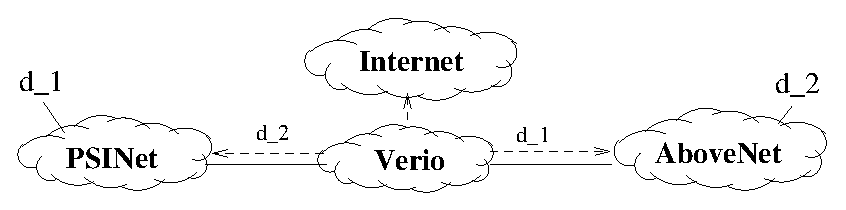
\includegraphics{figures/depeer.eps}}
%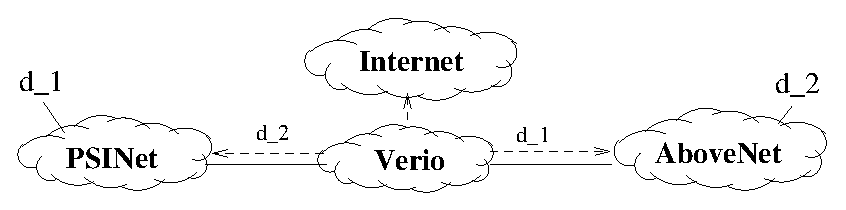
\epsfig{file=figures/depeer.eps,width=0.45\textwidth,height=0.9in}
\end{psfrags}
\caption{Constraints on filtering and topology are not enforceable. }
\label{fig:depeer}
\end{figure}

\begin{example}
\label{ex:depeer}
Figure~\ref{fig:depeer} shows a situation that occurred 
in 2001~\cite{bush:privcomm}.  When PSINet terminated
its peering with AboveNet, AboveNet lost connectivity to
PSINet's customers, $d_1$.  To restore connectivity, AboveNet
bought ``transit'' service from Verio (already a peer of PSINet), but
only for routes to PSINet and its customers.
%\footnote{Thanks to
%Randy Bush for this anecdote.}

%Verio treats AboveNet as a customer, advertising $d_1$ (and all of
%PSINet's prefixes) to AboveNet.  
Verio does not filter $d_1$ (or any of PSINet's prefixes) from AboveNet,
which is only possible if Verio treats AboveNet as a customer.
The constraints imposed by Gao and
Rexford state that an AS {\em must} prefer customer routes over peering
routes.\footnote{Gao and Rexford present a weaker constraint that allows
an AS to rank routes learned from customers and peers over those from
providers, but does {\em not} require customer routes to be strictly
preferred over routes from peers.  This relaxed condition requires that
there are no instances where an AS's customer is also a peer of another
one of the AS's peers.  Of course, the example shown in
Figure~\ref{fig:depeer} could also 
violate this 
constraint on the topology: PSINet is Verio's customer for $d_1$, but it
would be reasonable for PSINet to peer with another of Verio's peers,
since all are ``tier-1'' ISPs.}  
%
%The first constraint requires Verio to export a route to $d_3$ to the
%rest of the Internet (hence, requiring it to carry traffic to AboveNet's
%destination $d_3$ from {\em any} other network, not just
%PSINet).
%
This constraint requires Verio to rank AboveNet's route to $d_2$ over
any other available routes to $d_2$ in order to guarantee stability,
which restricts Verio's flexibility in how it can select
routes.
Establishing a new business
relationship (and, hence, altering its filtering policies) {\em requires} Verio
to change its rankings as well.
%
\end{example}



The framework of Gao and Rexford is also too strict because it assumes
that a pair of ASes has only a single type of business relationship. For
multinational ISPs, this assumption is constantly violated: two ASes may
have a peering relationship over sessions in one geographic region, but
one may purchase transit from the other in another geographic region.

\begin{figure}
\centering
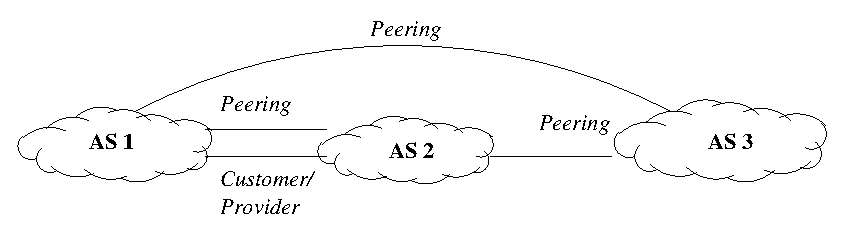
\epsfig{file=figures/peerprov.eps, width=0.8\linewidth}
\caption[Pairs of ASes may have different relationships
in different geographic regions.]{Pairs of ASes may have different
business relationships 
in different geographic regions.}
\label{fig:peerprov}
\end{figure}


\begin{example}
Consider Figure~\ref{fig:peerprov}; there are hundreds of similar
real-world examples~\cite{bush:privcomm}.  AS~1 and AS~2, two ISPs, peer
in North America, but AS~1 buys service from AS~2 in Europe (in
practice, this arrangement may occur if AS $1$ does not have a European
backbone).  AS~1 will typically learn {\em all} destinations (\ie,
European and North American) over its customer link, but just the North
American destinations over its peering link.  Suppose that AS~2 peers
with AS~3 in North America, and AS~1 peers with AS~3 in Europe.  The
router in AS~2 that has a peering relationship with AS~3 will advertise
the European routes from its customer link; AS~3 also learns those via
its peering session with AS~1.  This arrangement is precisely the
``peer-provider'' cycle that is prohibited some of the convergence
conditions of Gao and Rexford (\eg, Guideline A,~\cite{Gao2001a}).  This
scenario mandates that AS~2 prefer the route to the destination via
AS~1, rather than another peer through which it may have a route to the
same destination.
\end{example}


%% \noindent
%% This example demonstrates that the conditions suggested by Gao and Rexford
%% may be too strong to enable ASes to implement flexible
%% contracts.
%% %: according to these conditions, providing a
%% %service to AboveNet requires Verio to restrict both its ranking and its
%% %filtering.  
%% Hence, we are motivated to
%% study stability conditions for routing protocols, assuming that ASes are
%% completely 
%% unrestricted in how they filter.


Various previous work has studied {\em global} conditions to guarantee
the safety of routing systems; global conditions presume that the
routing system does not preserve local choice of rankings (\ie, ranking
autonomy).  Griffin \ea showed that, if the rankings of the ASes in
a routing system do not form a \emph{dispute wheel} (a concept that
describes global relationship between the rankings of a set of ASes),
then the routing system is safe~\cite{Griffin2002c}.  Griffin \ea also
examined {\em robustness}, the property that safety is guaranteed even
if arbitrary nodes or edges are removed from the graph.  We view
robustness as a special case of filtering: removing an edge can be
achieved if the ASes incident to that edge filter all routes through
that edge; removing a node entails having all ASes filter all routes
through that node.

%  Note that a dispute wheel
%does not fully characterize routing instability, because there are safe
%routing systems that have dispute wheels.  This paper presents a special
%case of a dispute wheel, called a dispute ring, and proves that a
%routing system with a dispute ring is unsafe under arbitrary filtering.
Griffin \ea also showed how to modify a BGP-like path vector protocol to
detect the existence of a dispute wheel but left unspecified how the
ASes should resolve the dispute wheel~\cite{Griffin2000}.  Machiraju and
Katz defined a new global invariant for determining safety when at most
one AS deviates from the conditions of Gao and
Rexford~\cite{Machiraju2004}.  Govindan \ea proposed a routing
architecture where ASes coordinate their policies~\cite{Govindan1999,
Govindan1998} using a standardized policy specification
language~\cite{rfc2622}.  Jaggard and Ramachandran presented
global conditions that guarantee safety of routing systems that allow
ASes to express only next-hop preferences over routes, and designed
centralized and distributed algorithms to check these global
conditions~\cite{Jaggard2004}.  

More recent work has attempted to design policy-based protocols that are
guaranteed to converge without imposing any global conditions.  Sobrinho
defined new concepts that describe global relationships between
preferences and incorporate several previous results (including those
of both Griffin \eans~\cite{Griffin2002c} and Gao and
Rexford~\cite{Gao2001a}) into a single algebraic
framework~\cite{Sobrinho2003}.  He examined requirements for
convergence and asserted that any vectoring protocol that preserves a
property called ``strict monotonicity'' is guaranteed to converge.
Recent work on ``metarouting'' exploits this algebraic framework to
allow protocol designers to specify new routing protocols that are
guaranteed to converge by requiring algebras that preserve strict
monotonicity~\cite{Griffin2005}.  In this chapter, we will
see that the set of routing protocols that are guaranteed to converge is
apparently not much more permissive than shortest path routing, if ASes
have complete liberty in setting filters.  Metarouting may allow the
protocol designer to better explore the tradeoffs between filtering
expressiveness, ranking expressiveness, and safety (\ie, compromising
filtering expressiveness to allow for more expressive rankings).

In contrast to these studies of global conditions for safety, we study
the conditions under which a policy-based interdomain routing protocol
can be safe if it preserves the autonomy of each AS.  Our results
suggest that, allowing for complete autonomy and filtering
expressiveness, guaranteeing safety requires restricting ranking
independence essentially to preferences based on consistent weightings
of the edges in the graph.

Gouda and Schneider study classes of routing protocol metrics for which
each node in a routing tree has its most preferred path, but do not
address routing stability~\cite{Gouda2003}.

%In constrast, we explore the necessary
%and sufficient conditions to guarantee stability while imposing only
%{\em local} constraints on an AS's rankings.  The results of our work
%suggest that imposing only local constraints to guarantee stability
%may require constraints that are too strong to allow sufficiently
%expressive routing policies.  As a result, the design of new
%interdomain routing protocols may require incorporating the types of
%global checks and algorithms described in this previous work.


% I say Who's on first, What's on second, I Don't Know's on third.
%- Lou Costello 


\qchapter{\textit{One of the beautiful things about baseball is that every once in a while you come into a situation where you want to, and where you have to, reach down and prove something.}  
    \vskip 0.1em - Nolan Ryan}{Correctness Specifications for Internet
    Routing}\label{chap:rlogic}


%\chapter{A Logic for Internet Routing}\label{chap:rlogic}

%% \cs{T}he complexity of Internet routing configuration and protocol
%% dynamics mandates a framework for understanding and manipulating
%% Internet routing at a level of abstraction that facilitates reasoning
%% about whether or not the protocol is behaving ``correctly''.  Naturally,
%% the first step in this process is defining what it means for a routing
%% protocol to operate correctly in the first place.  Specifying
%% correctness is not easy, because it requires distilling a high-level
%% description of how the routing protocol should behave from the myriad
%% technical minutia of the operation of the protocol.

\cs{T}he flexibility offered by Internet routing configuration
allows the protocol to scale well and enables operators to express a wide
variety of policies, but it increases the complexity of the system.  This
complexity makes it difficult to reason about the behavior of Internet
routing, leading to {\em ad hoc} fixes to observed problems that
ultimately only worsen this complexity.  Today, network operators (who
continually tweak routing configuration) and protocol designers
(who repeatedly propose ``point'' solutions to various problems) have
no way of reasoning about whether their modifications to Internet
routing will
operate as intended.  Worse yet, operators and designers do not even
have a {\em specification} of properties that Internet routing should
satisfy.  This chapter seeks to remedy this situation by specifying
correctness properties
that any routing protocol should satisfy.

We introduce three properties to
classify the behavior of a routing protocol.  We briefly describe
these properties below and explain why they are critical for
correct routing.

\begin{enumerate}
\itemsep=-1pt
\item {\em Route validity} states that if a router has a route to a
destination, then a usable path corresponding to that route exists in
the underlying topology.  If route
validity is violated, then end users could experience a failure of
end-to-end connectivity, because routers could forward packets along
non-existent paths.
%; for example, routers may ``blackhole'' traffic,
%or the traffic may get caught in a loop and may never reach the
%destination.
\item {\em Path visibility} states that if there is a usable path
between two nodes, then the routing protocol will propagate information
about that path.  A failure of path visibility could disrupt
end-to-end communication by preventing two connected nodes from learning
routes between one another.
\item {\em Safety} states that the routing protocol converges to a
stable route assignment, regardless of the order in which routing
messages are exchanged.  A routing protocol that violates safety will
induce persistent route oscillations, causing routing changes that
are unrelated to changes in topology or policy.
\end{enumerate}
\noindent
This chapter defines and investigates these properties and
demonstrates how they can 
deepen our understanding of network routing.
This correctness specification addresses {\em static} properties of
network routing, {\em not} dynamic behavior (\ie, its response to
changing inputs, convergence time, etc.). Internet routing, like any
distributed protocol, may experience periods of transient incorrectness
in response to changing inputs, but we are concerned with persistent
misbehavior.

Chapter~\ref{chap:rcc} presents an approach to detect when two
of these properties (route validity and path visibility) are violated.
Chapter~\ref{chap:sandbox} exploits
these properties to predict which
of many possible routes each router in the network will select.
Chapter~\ref{chap:policy} deals with the 
challenges of guaranteeing safety, an inherently global property.
%Chapter~\ref{chap:beyond} discusses how both dynamic analysis and
%routing protocol improvements can help guarantee these properties.

%Previous work in wide-area protocol design
%has focused on specific modifications to BGP that fix a particular
%problem but often spur unintended negative side effects.  Furthermore,
%designers of new wide-area routing protocols require a mechanism that
%enables them to reason about the circumstances under which the protocol
%will behave ``correctly''.  To help reason about modifications to
%existing routing protocols and to aid in the sound design of new ones in
%the future, we propose that routing protocols be classified in terms of
%specific high-level properties.

After we introduce some basic terminology in
Section~\ref{sec:definitions}, we motivate and describe the correctness
properties.  Sections~\ref{sec:validity_def},
\ref{sec:visibility_def},~and
\ref{sec:safety_def} 
describe route validity, path visibility, and safety, respectively, and
explain how various aspects of the operation and configuration
of the Internet's routing protocols can cause each of these to be
violated in practice.   

\section{Preliminaries: Paths, Routes, and Policy}\label{sec:definitions}

Before introducing the correctness properties themselves, we first
introduce some basic terminology for routing.  We explain these terms in
the context of Internet routing and BGP.  We first define paths and
routes in terms of a graph $G = (V,E)$, where the nodes in $V = \{v_1,
\ldots, v_N\}$ correspond to IP-level nodes (\ie, routers and end hosts)
and the edges in $E$ corresponds to IP-level links between those nodes.

\subsection{Paths and Routes}

We now define two basic terms---path and route---and explain how they
are related.
% We first define these terms generally.  Then,
%we discuss them using Internet routing as an example.

\begin{defn}[Path]\label{defn:rl:path}
A {\em path} is a sequence of nodes $P = (v_0, \ldots, v_n)$, where $v_i
\in G$ for all $0 \leq i \leq n$.
\end{defn}

\noindent
The definition of a path does not constrain how the sequence of nodes is
actually constructed.  As such, a path might represent a sequence of
directly connected IP-layer nodes or endpoints of a tunnel.\footnote{A
{\em tunnel} is a sequence of nodes that all forward packets to some
intermediate node (\ie, the tunnel's ``exit''), rather than the
ultimate destination.  A tunnel may be implemented by a variety of
mechanisms, such as IP-in-IP encapsulation~\cite{rfc2784}, Multiprotocol
Label Switching (MPLS)~\cite{davie:mplsbook,mpls-wg}, etc.}
Note that 
deleting some nodes from a path still results in a path.  
%For example, a path
%that is a sequence of tunnel endpoints can be constructed by taking the
%corresponding IP-layer path and deleting all nodes but the tunnel
%endpoints. A path could even even represent AS-level hops if it only
%included one IP-level hop per AS.

In contrast to a path, a route is {\em information} that allows nodes in
$G$ to construct paths to {\em destinations}.  The {\em destination} $d$
may refer either to a single node or a group of nodes (named, for
example, by an IP prefix).  The purpose of a routing protocol is to
propagate routes for destinations.  Collectively, the routes to $d$ that
the nodes in $G$ ultimately select define the {\em path} from any node
in $G$ to that destination.  All of our definitions presume that the
handle for a destination, $d$, cannot be manipulated (\eg, our
definitions do not consider the effects of IP prefix
aggregation~\cite{rfc1519,rfc1518}). 

\begin{defn}[Route]\label{def:route}
A {\em route} is a mapping $(d \rightarrow v_i)$, where $d$ is a
destination, and $v_i \in G$ is a node en route to the destination
$d$.  
\end{defn}
\noindent
We say that $v_i\in d$ if the destination $d$ includes $v_i$.  A route
$(d \rightarrow v_i)$ received by $v_j$ indicates that, if $v_j$ has a
packet to send to some node at destination $d$, it can forward that
packet to $v_i$, which in turn ought to have a route to $d$ (whereupon
this process repeats until the data reaches $d$).  One can think of a
route $(d \rightarrow v_i)$ being used at node $v_j$ as {\em inducing}
a path, $(v_j, \ldots, v_i)$, where either $v_j$ and $v_i$ are directly
connected or where the actual nodes along that path segment are
determined by the connectivity between those nodes, as established by the
IGP or using tunnels.  We will formalize the notion of induced paths in
Section~\ref{sec:consistency}.

Note that Definition~\ref{def:route} can apply to any routing protocol,
not just to BGP.  In an IGP, the node $v_i$ is typically the router that is
immediately connected at the IP layer.  In BGP, however, (particularly
in iBGP) the next hop may be several IP-layer hops away.  In
BGP, a node that receives a route $(d \rightarrow v)$ but is not
directly connected to $v$ must rely on the IGP for reachability to $v$.

\subsection{Induced Paths and Consistent Paths}\label{sec:consistency}

We can think of paths as being {\em induced} by routes.  That is, while
there exist many sequences of nodes between any node $v_0$ and a node in some
destination $d$, the path that traffic will actually take from $v_0$ en
route to $d$ is determined by the routes that the nodes in $G$ select.
In many routing protocols, including BGP, no single node has knowledge
about the entire sequence of nodes that traffic traverses en route to
$d$; rather, the
nodes that the routes select collectively {\em induce} a path to $d$.  We are
interested in making statements about those induced paths.  We now
formalize the concept of induced paths and describe a special class of
induced paths called {\em consistent paths}.

\begin{figure}
\centering
\begin{psfrags}
\psfrag{vi}{ $v_1$}
\psfrag{vid}{{\small $v_n \in d$}}
\psfrag{vi1}{$v_{i-1}$}
\psfrag{v0}{$v_0$}
\psfrag{v1}{$v_1$}
\psfrag{p1}{$P_{v_0}(r_{v_0}(v_i))$}
\psfrag{p2}{$P_{v_1}(r_{v_1}(d))$}
\psfrag{p3}{$P_{v_0}(r_{v_0}(d))$}
\resizebox{0.5\textwidth}{!}{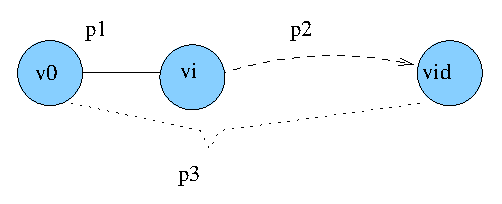
\includegraphics{rlogic/figures/induced_path1.eps}}
\end{psfrags}
%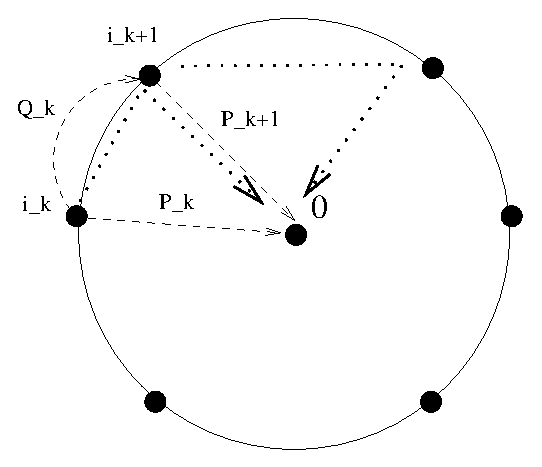
\epsfig{file=policy/figures/dw.eps,width=0.28\textwidth}
\caption[Illustration of an induced path.]{Illustration of an induced 
  path from $v_0$ to $d$, collectively induced by the selection of
  a route to $d$ at every node along the path.  The node $v_i$ may be
  immediately adjacent to $v_0$ (as shown), but it may also be several
  hops away.}
\label{fig:induced_path}
\end{figure}


\begin{defn}[Induced path]\label{defn:ipath}
Let $r_{v_j}(d)$ be the route that node $v_j$ selects en route to $d$
(\ie, it is a mapping $(d \rightarrow v_k)$ for some other $v_k\in G$.
Then, the {\em path induced} by route $r_{v_0}(d): (d \rightarrow v_i)$,
$P_{v_0}(r_{v_0}(d))$, is:
\[
P_{v_0}(r_{v_0}(d)) = \left\{\
\begin{array}{l}
\phi \textrm{ if $v_0$ has no route to $d$ }\\
v_0  \textrm{ if $v_0 \in d$}\\
%(v_0, P_{v_0}(r_{v_0}(v_i)), P_{v_i}(r_{v_i}(d))) \textrm{ otherwise }
(v_0, P_{v_1}(r_{v_1}(d))) \textrm{ otherwise }
\end{array}
\right.
\]
where $v_1$ is defined according to $r_{v_0}(v_i): (d \rightarrow v_1)$;
that is, $v_1$ is the next-hop node in $v_0$'s forwarding table for
destination $v_i$.
\end{defn}

\noindent
Figure~\ref{fig:induced_path} illustrates an induced path and its
constituent subpaths.  The node $v_i$ in the induced path may either be
adjacent to $v_0$ in $G$, or it may be several hops away.  When $v_i$ is
adjacent to $v_0$ in $G$, data traffic can reach $v_i$ from $v_0$ via a direct
IP link.  When $v_i$ is several hops away in $G$, however, $v_0$ must
rely on intermediate nodes to forward traffic to $v_i$.  In this case,
the nodes between $v_0$ and $v_i$ could 
use routes that induce paths that never even traverse $v_i$.
In other words, the path that is described by $(v_0,
P_{v_0}(r_{v_0}(v_i)))$ may traverse an intermediate node whose induced
path to $d$ does not traverse $v_i$.  To precisely
classify the types of paths for which 
this inconsistency does not arise, we define the notion of a consistent
path.

\begin{defn}[Consistent path]
An induced path $P_{v_0}(r_{v_0}(d)) = (v_0, \ldots v_n)$ to $d$ is consistent
if, (1)~for all $1 \leq i \leq n$, $P_{v_i}(r_{v_i}(d)) = (v_i, v_{i+1},
\ldots, v_n)$; (2)~$P_{v_0}(r(v_0(d)))$ contains $v_i$, where
$r_{v_0}(d): d \rightarrow v_i$.
\end{defn}

Consistent paths are an important class of paths because inconsistent
paths can sometimes give rise to forwarding loops.  A {\em forwarding
loop} is a special case of an inconsistent path where some intermediate
node's induced path includes a node that has already appeared on the
path.  

When $v_0$ and $v_i$ are not adjacent, ensuring that all intermediate
nodes select a route $(d\rightarrow v_i)$ will guarantee that an induced
path is consistent.  If an intermediate node selects some route
$(d\rightarrow v_j)$ where $v_i\neq v_j$, then the induced path to $d$
may never traverse $v_i$.  If, on
the other hand, the intermediate node selects a route $(d\rightarrow
v_i)$, then the induced path from that node to $v_i$ will be a subpath
of $P_{v_0}(r_{v_0}(v_i))$, assuming all nodes use the same function to
induce paths (\eg, if the induced path to $v_i$ is based on shortest
paths routing, as in an IGP).


%\subsection{Example: Paths and Routes in Internet Routing}

We now briefly discuss paths and routes in the context of BGP.  To
illustrate the distinction between routes and paths, we examine their
definitions within the context of BGP routing within a single AS.  In
this case, a {\em route} is of the form $(d \rightarrow v_i)$, where $d$
is an IP prefix and $v_i$ is the BGP ``next hop'' (a node that need not
be directly connected at the IP layer).  The {\em path} that traffic
ultimately takes from some node $v_j$ to the destination $d$, for which
$v_j$ has a route $(d \rightarrow v_i)$, depends on how connectivity is
established between $v_j$ and $v_i$.  If $v_j$ and $v_i$ are in two
different ASes, then they are typically directly connected.  If they are
in the same AS, however, it is common for $v_i$ to be the IP address of
an egress (or ``border'') router and for $v_j$ to be several IP hops
away.  The induced path between $v_j$ and $v_i$ may be determined by a
tunnel, by a shortest paths routing protocol, using static routes, etc.

If the induced path between $v_j$ and $v_i$ is not defined by a tunnel,
then the nodes between $v_j$ and $v_i$ will use their own routes for
forwarding data to $d$.  In this case, the induced path to $d$ is
actually determined by ``stitching together'' these constituent induced
paths.  If all nodes between $v_j$ and $v_i$ select routes that indicate
that traffic to $d$ should be sent via $v_i$, then the induced path
between $v_j$ and $v_i$ will be consistent.  Otherwise, the path could
be arbitrary; in fact, it might never traverse $v_i$.

\begin{figure}
\centering
\begin{psfrags}
\psfrag{v1}{{\LARGE $v_1$}}
\psfrag{v2}{{\LARGE $v_2$}}
\psfrag{v3}{{\LARGE $v_3$}}
\psfrag{v4}{{\LARGE $v_4$}}
\psfrag{v5}{{\LARGE $v_5$}}
\psfrag{d}{{\LARGE $d$}}
\psfrag{dr}{{\Large $(d \rightarrow v_5)$}}
%
%\hspace{-0.7in}
\resizebox{0.65\textwidth}{!}{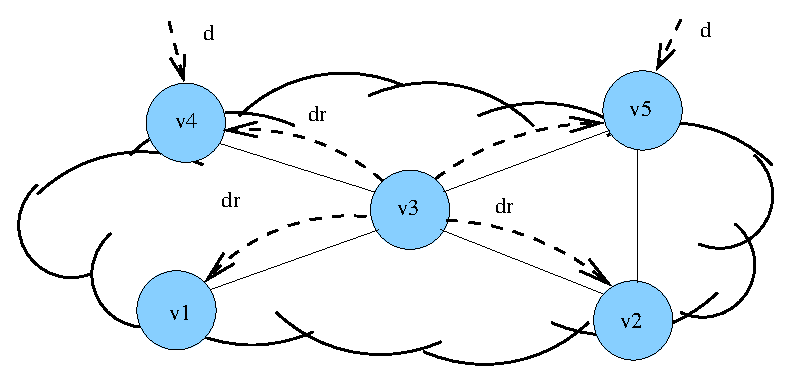
\includegraphics{rlogic/figures/path_route.eps}}
\end{psfrags}
%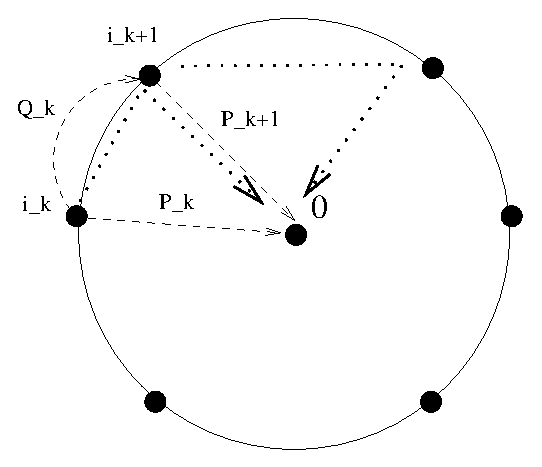
\epsfig{file=policy/figures/dw.eps,width=0.28\textwidth}
\caption[Paths and routes in BGP.]{An example that demonstrates how BGP
  routes induce paths.  Dashed lines are iBGP sessions from route
  reflectors to clients (\ie, $v_3$ is a route reflector, and the rest of
  the routers are its clients); route reflector operation is summarized
  in Section~\ref{sec:dissemination}.  Dashed lines show propagation of
  routes. Solid lines show IGP links; in this example, all links have a
  cost of $1$.  The routes at each node {\em induce} paths over the IGP
  topology. For example, the induced path from $v_2$ to $d$ is $(v_2,
  v_5, ...)$, the induced path from $v_1$ to $d$ is $(v_1, v_3, v_5,
  ...)$, etc.}
\label{fig:path_route}
\end{figure}

Figure~\ref{fig:path_route} shows an example that illustrates this
distinction.  In this example, all routers in the AS are clients of the
route reflector, $v_3$; solid lines show the edges in the IGP graph, and
all edges have a cost of $1$.  Suppose that $v_3$ learns two routes to
$d$ and selects the route that it receives from $v_5$.  In this case,
$v_3$ propagates that {\em route} (\ie, $(d \rightarrow v_5)$) to all of
its clients, as shown.   Using that route, each node ultimately uses a
different {\em path} to the egress router, $v_5$.  For example, $v_1$'s
shortest IGP path to $v_5$ is $v_1,v_3,v_5$, whereas $v_2$'s shortest
path to $v_5$ is $v_2, v_5$.  Even if a node, say $v_1$ selects a BGP
route with the ``next hop'' $v_5$, there is no guarantee that the
resulting {\em induced path} will traverse $v_5$.  If an additional
node, $v_6$, 
had been on the path between $v_1$ and $v_3$, and had instead selected a
route $(d\rightarrow v_4)$, then $v_1$'s path to $d$ through the AS
could have in fact been $v_1, v_6, v_4$.




%For the pursposes of our work, we assume that physical
%links and internal routing is operating correctly.  That is, we assume
%that a path exists between {\em any} source-destination pair where the
%source and destination are in the same AS.

\subsection{Policy}

A noteworthy aspect of Internet routing is that it is {\em policy-based}.
The job of the routing protocol is not to propagate complete
information about the topology, but to only propagate information about
paths that comply with the various economic and policy goals of each AS.
We must therefore qualify paths in the topology according to
those that comply with such these policies and those that do not.

\begin{defn}[Policy]\label{defn:policy}
A {\em policy} is a function $\P(s, v_{i-1},v_{i},v_{i+1},d) \rightarrow
(0,1)$, 
where $s$ is a source, $v_{i-1}$, $v_i$, and $v_{i+1}$ are 
nodes on a path $(v_0, v_1, \ldots, v_n)$, $d$ is a
destination, and $\P$ is defined as follows: 
\[
\P(s,v_{i-1},v_i,v_{i+1},d) = \left\{\
\begin{array}{l}
1\textrm{ if $i=0$ and $v_0$ forwards packets from source $s$ destined
  for $d$}\\ 
1\textrm{ if $0<i<n$ and $v_i$ forwards packets with source $s$ from
  $v_{i-1}$} \\ \textrm{\hspace*{0.2in} destined for $d$ via $v_{i+1}$}\\
1\textrm{ if $i=n$ and $v_n$ forwards packets with source $s$ destined
  for $d$}\\ 
0\textrm{ otherwise }
\end{array}
\right.
\]
\end{defn}

The function $\P(v_{i-1}, v_i, v_{i+1}, d)$ is not expressive enough to
capture all policies, but, as we will see, it is general enough to
capture the policies that are commonly expressed in Internet
routing.  Other routing protocols may require more expressive
policy functions. Our intent here is not to define a policy function
that captures all policies, but rather to allow us to define a
policy-conformant path in the context of Internet routing.

%A value of $0$ indicates that traffic
%should not be allowed to flow on any path from $s$ to $d$; a value of
%$1$ indicates that such a path is permissible.

\begin{defn}[Policy-conformant path]\label{defn:pcp}
A path $(v_0, v_1, v_2, \ldots, v_n)$ is policy-conformant for source $s$
and destination 
$d$ if $\P(s, v_{i-1}, v_i, v_{i+1},d) = 1$ for all $0 \leq i \leq n$.
\end{defn}

\noindent
For simplicity, we assume that paths for which the source,
destination, and all nodes in between the source and destination are in
the same AS are policy-conformant.  
%

\begin{figure}
\centering
\begin{psfrags}
\psfrag{X}{{\Large $X$}}
\psfrag{Y}{{\Large $Y$}}
\psfrag{Z}{{\Large $Z$}}
\psfrag{vx}{$v_X$}
\psfrag{vy1}{$v_i$}
\psfrag{vy2}{$v_j$}
\psfrag{vz}{$v_Z$}
\resizebox{0.9\textwidth}{!}{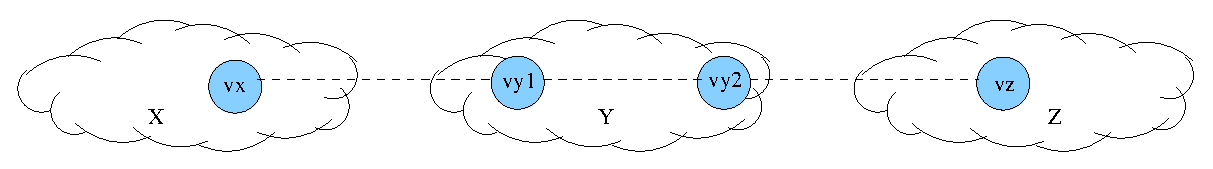
\includegraphics{rlogic/figures/policy_ex.eps}}
\end{psfrags}
\caption[Expressing policy-conformant paths at the AS-level in BGP.]{An example
  illustrating policy-conformant paths at the AS-level in BGP.}
\label{fig:policy_ex}
\end{figure}


%The policy function $\P$ allows an operator to restrict paths that do
%not conform to some policy by expressing $\P(v_{i-1},v_i,v_{i+1},d)$,
%where $v_{i-1}$, $v_i$, and $v_{i+1}$ are nodes in three different ASes.
Although the policy function is defined at the level of nodes, it is in
fact expressive enough to capture many AS-level policies that network
operators commonly want to express.  For example, suppose an operator
wants to express that AS $Y$ should not forward traffic between two other
ASes, $X$ and $Z$, for some destination $d$, as
pictured in Figure~\ref{fig:policy_ex}.  Recall that a path with some
nodes removed still constitutes a path.  As such, it is possible 
to express this policy in terms of the nodes in ASes $X$ and $Z$
along the path.  For example, in Figure~\ref{fig:policy_ex}, the policy can be
expressed as $\P(s, v_X, v_i, v_Z, d) = 0$.  In a more complicated
scenario, if AS $Y$ has multiple nodes that are adjacent to nodes in
ASes $X$ and $Z$, the AS-level policy would be
expressed as an enumeration over node-level policies.



\section{Route Validity}\label{sec:validity_def}

In this section, we motivate and describe {\em route validity}.
Informally, route validity says that any route that the routing protocol
propagates should correspond to a usable path in the topology.  Route
validity concerns the properties of the paths induced by the routes that
the routing protocol propagates.

\begin{defn}[Route validity]\label{defn:rv}
A route for a destination $d$ is valid if, and only if, the path induced
by the route (1)~is consistent, (2)~is policy-conformant for all sources
that use the route, and
(3)~terminates at $d$.  We say that a routing protocol satisfies route
validity if the protocol propagates only valid routes for all
destinations.
\end{defn}


\begin{figure}
\centering
\begin{psfrags}
%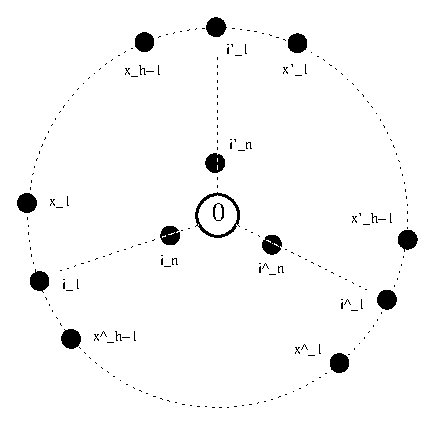
\epsfig{file=policy/figures/lemdr.eps,width=0.25\textwidth}
%
\psfrag{vi}{ $v_i$}
\psfrag{vid}{ $v_n \in d$}
\psfrag{vnd}{ $v_n \in d$}
\psfrag{vi1}{$v_{i-1}$}
\psfrag{v0}{$v_0$}
\psfrag{v1}{$v_1$}
\psfrag{dr}{$(d \rightarrow v_i)$}
\psfrag{d}{$d$}
%
%\hspace{-0.7in}
\resizebox{\textwidth}{!}{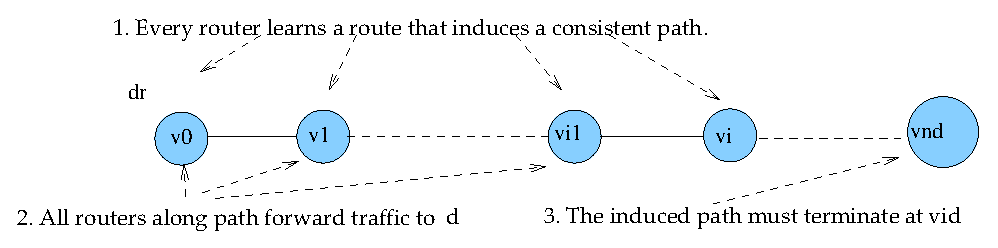
\includegraphics{rlogic/figures/rv_expl.eps}}
\end{psfrags}
%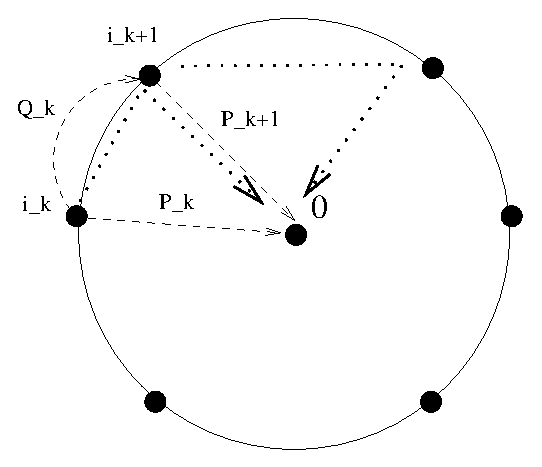
\epsfig{file=policy/figures/dw.eps,width=0.28\textwidth}
\caption[The conditions of route validity.]{The conditions of route
  validity.  A route is valid if it induces a consistent,
  policy-conformant path at every node along the path from $v_0$ to some
  $v_i \in d$.}
\label{fig:rv_expl}
\end{figure}


Figure~\ref{fig:rv_expl} illustrates the conditions of route validity.
The first condition of route validity enforces consistency
along the path between $v_0$ and the node $v_i$ towards which $v_0$
sends traffic en route to $d$.
%If all intermediate nodes
%between $v_0$ and $v_i$ have the same next-hop, $v_i$, then there can be
%no forwarding loops between $v_0$ and $v_i$.  
Furthermore, the induced path from $v_0$ to $v_i$ must be
policy-conformant; that is, every node along the path $(v_0, \ldots, v_i)$
must forward traffic from its predecessor to its next hop en route to
$d$.  Verifying policy conformance is difficult for
paths that traverse multiple ASes, because operators do not explicitly
specify the policy function $\P$.  The final condition says that the
path induced by the route must actually terminate at some node $v_n \in
d$.
%The final condition of route validity says that, once
%traffic reaches the node $v_i$, then that node also has a route to the
%destination that satisfies route validity.


%%%%%%%%%%%%%%%%%%%%%%%%%%%%%%%%%%%%%%%%%%%%%%%%%%%%%%%%%%%%

Because a source $v_0$ and a destination $d$ may be in different ASes,
guaranteeing that BGP satisfies route validity is difficult in practice.
Determining both the induced path to $d$ and determining whether that
path is policy-conformant requires knowledge of the configurations of
multiple ASes.  Fortunately, the properties of route validity (\ie,
consistency and policy-conformance) are composable.

\begin{observation}\label{obs:composable}
Composing a path by concatenating two consistent, policy-conformant
paths results in a new consistent, policy-conformant path.
\end{observation}

This observation implies that if the routing protocols in each AS en
route to a destination induce only consistent and policy-conformant
paths to some destination $d$, then BGP will only induce consistent,
policy-conformant paths for that destination $d$.  For the purposes of
this chapter, we assume that all paths are policy-conformant, because
detecting violations of policy are difficult to verify in practice; we will
return to this issue in Section~\ref{sec:validity}.  We also assume that
all eBGP sessions are point-to-point (\ie, immediately connected at the
IP layer), which is almost always the case in practice: service
providers typically apply policies at AS boundaries, rather than on
paths within an AS.  Finally, we assume that the IGP already satisfies
route validity; detecting route validity faults in internal routing
protocols is beyond the scope of this dissertation.



%% \begin{proof}
%% We must show that, when a route gives rise to a path where any $v_i$ and
%% $v_{i+1}$ are in different ASes, then the path that traverses the two
%% ASes still satisfies the conditions for route validity.  Since the path
%% segment $v_i, v_{i+1}$ is a point-to-point link, then $v_i$ selects the
%% route $(d \rightarrow v_{i+1})$, and the first condition is satisfied.
%% The third condition is satisfied by the inductive assumption.  
%% \end{proof}


Modulo policy-conformance, guaranteeing that BGP satisfies route
validity boils down to ensuring that iBGP always induces consistent
paths within each AS.  Guaranteeing this property is the focus of
the remainder of this section.  We first focus on how to guarantee that
``full mesh'' iBGP configurations (and protocol modifications that
would allow every
router to the complete set of ``best'' eBGP-learned routes) always
induce consistent paths; we 
then derive conditions on iBGP configurations that use route reflection
that guarantee that iBGP only induces consistent paths.

\subsection{Case \#1: Every router learns all ``best'' eBGP routes.}
\label{sec:mesh}

If different routers within an AS receive different sets of candidate
routes for some destination $d$, then the routers along a path from $v_0$
to $v_i$ may not ultimately select the route $(d \rightarrow v_i)$.  It
turns out that the default iBGP configuration, where every eBGP-speaking
router has an iBGP session with every other eBGP-speaking router in the
AS (\ie, a ``full mesh'' iBGP configuration, as described in
Section~\ref{sec:dissemination}, Figure~\ref{fig:fullmesh}) satisfies
route validity.

\begin{figure}
\centering
\begin{psfrags}
%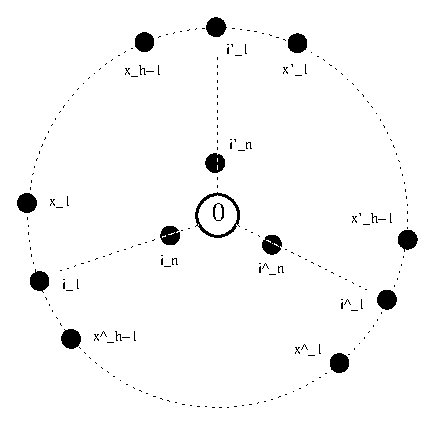
\epsfig{file=policy/figures/lemdr.eps,width=0.25\textwidth}
%
\psfrag{v_i}{{\LARGE $v_i$}}
\psfrag{v_j}{{\LARGE$v_j$}}
\psfrag{a}{{\LARGE $a$}}
\psfrag{b}{{\LARGE$b$}}
\psfrag{s}{{\LARGE$v_0$}}
%
%\hspace{-0.7in}
\resizebox{0.5\textwidth}{!}{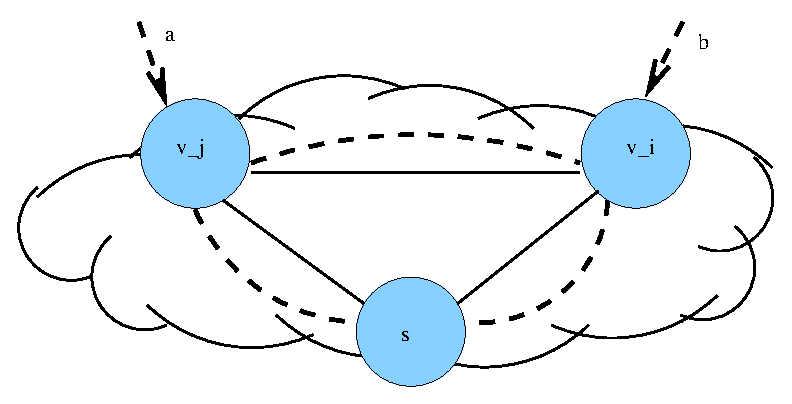
\includegraphics{rlogic/figures/fm_validity.eps}}
\end{psfrags}
%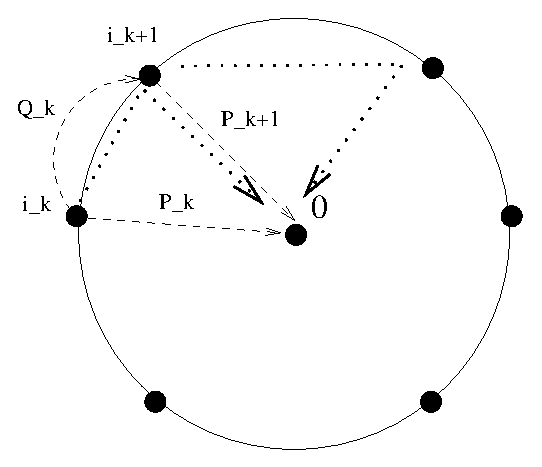
\epsfig{file=policy/figures/dw.eps,width=0.28\textwidth}
\caption[The main idea of the proof of
  Theorem~\ref{th:mesh}]{This figure illustrates the main idea of the proof of
  Theorem~\ref{th:mesh}.  Dashed lines represent iBGP sessions, and
  solid line represent IGP links.  If routes $a$ and $b$ do not have equal
  local preference, AS path length, origin type, or MED, then $v_0$,
  $v_i$, and $v_j$ will all select the same route.  If these attributes
  are equal for both $a$ and $b$, then $v_0$ selects either $a$ or $b$
  depending on whether $v_i$ or $v_j$ has a shorter IGP path.  If $v_j$
  selects route $a$ and $v_i$ selects route $b$, then $v_0$'s shortest IGP
  path to the next hop corresponding to the chosen route must be direct.}
\label{fig:fm_validity}
\end{figure}


\begin{theorem}\label{th:mesh}
If (1)~every router learns the BGP routes selected by the complete set of
eBGP-speaking routers, and
(2)~iBGP-speaking routers do not modify route attributes (\ie, local
preference, origin type, MED, or next hop), then 
all paths induced by iBGP (within the AS) will be consistent.
\end{theorem}

\begin{proof}
If each router eventually learns of the route selected by every
eBGP-speaking router, then there are two cases for any router $v_0$ in
the AS: either (1)~$v_0$ selects a route via a $v_i$ in a neighboring
AS, or (2)~$v_0$ selects a route via $v_i$ in the same AS, where $v_i$ is an
eBGP-speaking router and, hence, in turn selects a route such that
$v_{i+i}$ is in a neighboring AS.  The first case corresponds to a
point-to-point eBGP session; the second case corresponds to an iBGP
session where the route's next hop $v_i$ learned the route via a
point-to-point eBGP session but may be multiple IP hops away.  For the
proof of this theorem, we are only concerned with the latter case; we
rely on Observation~\ref{obs:composable} to ensure that iBGP induces
only consistent paths in neighboring ASes.

%% Route validity holds in the first case, because $v_i$ is in a
%% neighboring AS, and, by assumption, the remainder of the path is
%% consistent.  In the case where $v_i$ is in the same AS, the path $(v_0,
%% \ldots, v_i)$ may include multiple nodes (\ie, routers) in the same AS.
%% We know that $v_i$ selects a route that induces a consistent path
%% because $v_i$ selects a route from a neighboring AS.  

To show that iBGP induces only consistent paths within the AS, we show
that all routers on the path $(v_0, \ldots, v_i)$ select the route $(d
\rightarrow v_i)$, for any $v_i\in G$.  Because all eBGP-speaking
routers have an iBGP session with every other router in the AS, all
routers (and, in particular, all routers along the path $(v_0, \ldots,
v_i)$) learn the same set of ``best'' routes.  All of these routers
would thus select a route with the highest local preference, shortest AS
path length, lowest origin type, and lowest MED.

As a result, we know that all routers along the path $(v_0, \ldots,
v_i)$ select {\em some} iBGP learned route with the shortest IGP path
among candidate iBGP routes.  Suppose that some router on this path, say
$v_j$, selects a route other than $(d \rightarrow v_i)$, say $(d
\rightarrow v_k)$, because $(v_j, \ldots, v_k)$ has a shorter path cost
than $(v_j, \ldots, v_i)$.  Then, the nodes in $(v_0, \ldots, v_k)$ {\em
also} have a shorter IGP path cost than $(v_0, \ldots, v_i)$ and, hence,
all nodes in $(v_0, \ldots, v_{k-1})$ would also select $(d \rightarrow
v_k)$.
\end{proof}

A full mesh iBGP configuration can guarantee the first condition of
Theorem~\ref{th:mesh}.  Another approach to ensuring that every router
learns the set of routes selected by the complete set of eBGP-speaking
routers is to alter how route reflectors readvertise routes to their
clients.  By a similar argument as in the proof of
Theorem~\ref{th:mesh}, such a modification would cause iBGP to induce
only consistent paths.  Such a configuration not only guarantees
consistent paths, but it also prevents certain types of persistent route
oscillation (a pathology we examine in more detail in
Section~\ref{sec:safety_def})~\cite{Basu2002}. Unfortunately,
implementing such a configuration in practice requires modifying the
large deployed base of BGP routers.  Alternatively, an architecture such
as either the Routing Control Platform
(RCP)~\cite{caesar2004,feamster:fdna2004} or the recent proposal for
more versatile route reflectors~\cite{id-versatile-rr} could implement
this type of iBGP configuration.


%% \begin{defn}[RR-Reflect-All]
%% A route reflector configuration for an AS is {\em RR-Reflect-All} if all
%% route reflectors for that AS advertise all routes to a particular
%% destination (as opposed to simply the best route), and route reflectors
%% readvertise all routes with each other (\ie, path visibility is
%% satisfied among router reflectors).
%% \end{defn}

%% \begin{theorem}\label{th:rr_reflect}
%% If the route reflectors in an AS are configured according to {\em
%% RR-Reflect-All}, then all paths induced by iBGP are consistent.
%% \end{theorem}

%% \begin{proof}

%% In an {\em RR-Reflect-All} iBGP configuration, all routers ultimately
%% receive all routes to a destination $d$.  There are two cases:
%% (1)~there exists only one route that is better according to the first
%% four steps of the BGP route selection process (local preference, AS path
%% length, 
%% origin type, MED); (2)~there exists more than one route to $d$, and ties
%% between multiple candidate routes are broken after the first four steps.
%% In the first case, all routers will select that single route with common
%% next hop, so route validity is satisfied because every router selects
%% the same next hop.  In the second case, either a router $v_0$ selects a
%% route via its own eBGP session, if one exists (in which case route
%% validity is trivially satisfied again) or it selects a route that
%% traverses other routers in the same AS to reach the next hop $v_i$.
%% Because every router receives all routes to a destination, if some
%% router on the shortest path between $v_0$ and $v_i$ selects a route with a
%% next-hop other than $v_i$, then $v_0$ would have also selected the route
%% with that next hop, by the same argument in Theorem~\ref{th:mesh}.
%% \end{proof}





\subsection{Case \#2: Each router learns only some ``best'' eBGP routes}

If full mesh iBGP were the only intra-AS BGP configuration,
guaranteeing that iBGP satisfied route validity would be easy.
Unfortunately, as discussed in Section~\ref{sec:dissemination}, this
technique does not scale to large ASes because it requires $O(|R|^2)$
iBGP sessions, where $|R|$ is the number of routers in the AS.  Large
ASes typically use a 
technique called route 
reflection, where a single route reflector selects a route on behalf of
its client routers.


\begin{figure}
\begin{center}
\begin{psfrags}
\psfrag{RR1}{{\LARGE $RR_1$}}
\psfrag{RR2}{{\LARGE $RR_2$}}
\psfrag{C1}{{\LARGE $C_1$}}
\psfrag{C2}{{\LARGE $C_2$}}
\psfrag{d}{{\LARGE $d$}}
%\centering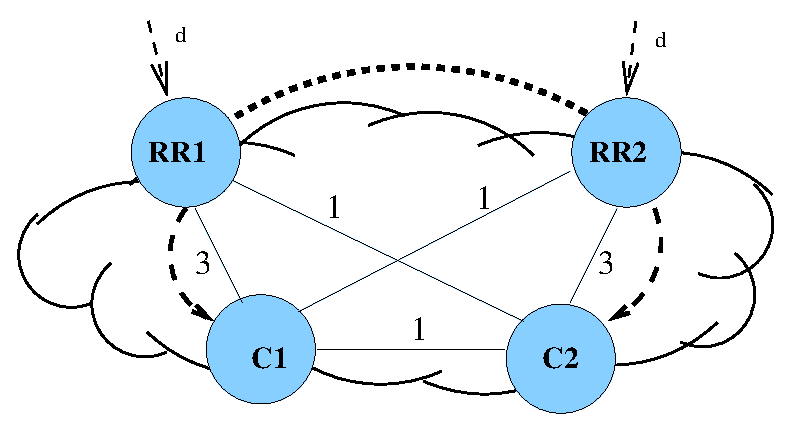
\epsfig{file=rlogic/figures/dube.eps,width=0.7\textwidth}
\resizebox{0.5\textwidth}{!}{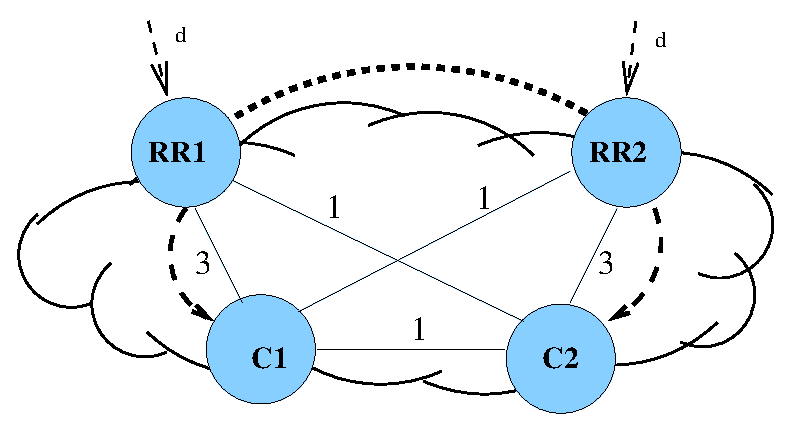
\includegraphics{rlogic/figures/dube.eps}}
\end{psfrags}
\end{center}
\caption[The interaction of IGP and route reflection may cause
  forwarding loops.]{The interaction of IGP and route reflection in iBGP
  may cause route validity violations resulting in forwarding
  loops~\cite{Dube99}. 
  Note that this topology satisfies path visibility but not route
  validity.  Dashed lines represent iBGP sessions; a directed edge
  indicates an iBGP sessions from a route reflector to its client.}
\label{fig:dube}
\end{figure}


Guaranteeing route validity in an iBGP topology with route reflectors is
not easy.  Previous work has observed that the interactions between the
IGP topology and an iBGP topology with route reflectors can give rise to route
validity violations~\cite{Dube99}.  Figure~\ref{fig:dube} shows one such
example.  Route reflectors $RR_1$ and $RR_2$ both receive a route to
destination $d$ and have clients $C_1$ and $C_2$ respectively.  Hence,
$C_1$ may receive and select the route $(d \rightarrow RR_1)$, and $C_2$
may receive and select the route $(d \rightarrow RR_2)$.  If the
shortest IGP path (\ie, the induced path) between $A$ and $RR_1$ is via
$B$, and the shortest 
IGP path between $B$ and $RR_2$ is via $A$, then traffic en route to $d$
that traverses either router $A$ or $B$ will be caught in a persistent
{\em forwarding loop}: that is, traffic destined for $d$ will never
reach $d$ but instead will repeatedly visit a cycle of two or
more nodes.  A forwarding loop is simply a special case of a route
validity violation.

Our goal is to detect whether a configuration of route reflectors and
clients induces only consistent paths with a simple algorithm that
examines only the static iBGP and IGP topologies.  One such sufficient
condition that guarantees this property requires that the iBGP topology
be {\em RR-IGP-Consistent}, defined as follows:

\begin{defn}[RR-IGP-Consistent]\label{defn:igp-consistent}
A route reflector configuration is {\em RR-IGP-Consistent} if, for all
nodes, every shortest IGP path between that node and its possible egress
nodes (\ie, the set of eBGP-speaking routers) traverses that node's
route reflector before any other node's route reflector and the egress
node's route reflector before the egress node itself.
\end{defn}
In previous work, Dube suggested placing route
reflectors on the shortest IGP path to their clients~\cite{Dube99}.  We
now prove that this condition guarantees that the iBGP configuration
will only induce consistent paths.  

\begin{theorem}\label{th:rr_safe}
If an iBGP configuration is {\em RR-IGP-Consistent}, then
all paths induced by iBGP are consistent.
\end{theorem}

\begin{proof}
Suppose not.  Then, there must exist a
destination $d$ and a path $P = (v_0, \ldots, v_n)$ for which some node $v_j$
between $v_0$ and $v_n$ selects a route $(d \rightarrow v_i)$, where $i
\neq n$.  There are two cases: (1)~$v_j$ is on the path from $v_0$ to the
route reflector of $v_0$; and (2)~$v_j$ is on the path from the route
reflector of $v_0$ to $v_n$.  

In the first case, if $v_0$ and $v_j$ select different next hops then, by
definition, they must be clients of different route reflectors.
By definition, then, the iBGP topology is not {\em RR-IGP-Consistent}.
%Then,
%it must be the case that either $v_0$'s path to $v_n$ goes through $v_j$'s
%route reflector before its own route reflector, or $v_j$'s path to $v_n$
%goes through $v_0$'s route reflector before its own route reflector.
%Either case implies that {\em RR-IGP-Consistent} is not satisfied.
The second case reduces to a similar argument as in
Theorem~\ref{th:mesh}: if $v_j$ selects a route with a next hop other
than $v_n$, then the route reflector of $v_0$ would have also learned that
route and selected it (otherwise, $v_j$ would not have been on the route
reflector's shortest path to $v_n$, by the same argument as in
Theorem~\ref{th:mesh}).
\end{proof}

Although this result is a helpful sufficient condition, it does not
guarantee that route validity will be satisfied when arbitrary links
fail, thus causing shortest IGP paths to change.  Designing an {\em
RR-IGP-Consistent} iBGP topology that is robust to link failures is a
difficult task.  Recent work has proposed using graph separators as a
way of efficiently placing route reflectors in an iBGP topology 
to guarantee that route validity is satisfied~\cite{Vutukuru2005}.  


%%%%%%%%%%%%%%%%%%%%%%%%%%%%%%%%%%%%%%%%%%%%%%%%%%%%%%%%%%%%

\section{Path Visibility}\label{sec:visibility_def}

Path visibility says that if there exists one or more policy-conformant
paths between two 
nodes, then the routing protocol should propagate routes that 
induce at least one of those paths.  Path visibility is an important
property for a number of reasons.  First, if a routing protocol
satisfies this property, then every node is guaranteed to have the
necessary information to reach all other nodes.
%Essentially, it states that the routing protocol is propagating
%enough information to allow any node to reach any other node for which
%it has a path in the underlying topology.  
%Second, as is evident from the
%theorems of Section~\ref{sec:validity_def}, an iBGP configuration must
%satisfy path visibility in order to satisfy route validity.

\begin{defn}[Path visibility]\label{defn:pv}
A routing protocol satisfies {\em path visibility} if, for all $v_0\in
V$ and for all destinations $d$, the existence of a policy-conformant
path $P = (v_0, \ldots, v_n)$ implies that $v_0$ learns a valid route
$(d \rightarrow v_j)$ for some $0 \leq j \leq n$.
\end{defn}

Path visibility states that if there is a policy-conformant
path from $v_0$ to $d$, then $v_0$ should learn {\em at least one} valid
route to $d$.  Note that the definition does not require $v_0$ to learn
all routes to $d$, nor does it require that $v_0$ learn the ``best''
route to $d$ by any metric.  Path visibility also does not require that
the route that $v_0$ learns correspond to the actual path that traffic
takes from $v_0$ to $d$.
%Although these might all be
%desirable properties, path visibility only requires the minimal
%conditions for correctness: as long as there is a policy-conformant path
%from $v_0$ to $d$, the routing protocol should propagate information that
%allows $v_0$ to send traffic to $d$.

By definition, path visibility violations result when some router fails
to propagate usable routes. These failures in route propagation 
range from the mundane (\eg, misconfigured filters that fail to
install or advertise routes for a policy-conformant path) to the subtle
(\eg, errors in iBGP configuration).

\begin{figure}
\begin{center}
\begin{psfrags}
\psfrag{R1}{{\LARGE $RR_1$}}
\psfrag{R2}{{\LARGE $RR_2$}}
\psfrag{R3}{{\LARGE $RR_3$}}
\psfrag{X}{{\LARGE $C_1$}}
\psfrag{Y}{{\LARGE $C_2$}}
\psfrag{Z}{{\LARGE $C_3$}}
\resizebox{0.6\textwidth}{!}{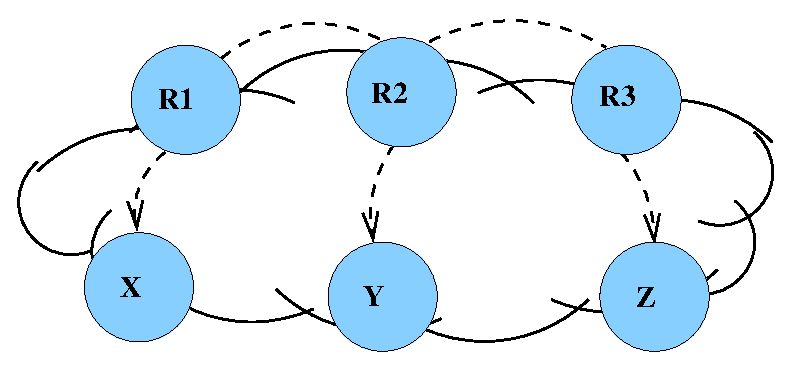
\includegraphics{rlogic/figures/ibgp_rr_pv.eps}}
\end{psfrags}
\end{center}
\caption[A simple iBGP topology that violates path visibility.]{A simple
  iBGP topology that violates path visibility.  Routes learned via eBGP
  at $RR_1$ or $C_1$ will not be propagated to $RR_3$ or $C_3$ (and vice
  versa).}
\label{fig:rl:ibgp_rr}
\end{figure}


Because of the way iBGP readvertises routes, an arbitrary iBGP
configuration is not guaranteed to satisfy path visibility.  In fact,
even the very 
simple iBGP topology in Figure~\ref{fig:rl:ibgp_rr} does not satisfy
path visibility: if the route reflector $RR_1$ (or its client, $C_1$)
receives a route for some destination via an eBGP session, then neither
$RR_3$ nor $C_3$ will receive a route to the destination, and vice
versa.  


Path visibility is important because it ensures that, if the network
remains connected at lower layers, the routing protocol does not create
any new network partitions.  Path visibility also reduces the likelihood of
suboptimal routing.  For example, in Figure~\ref{fig:rl:ibgp_rr}, even if
all clients learned {\em some} route to the destination via eBGP, the
clients would not be guaranteed to discover the {\em best} route to the
destination (\eg, if a client of the route reflector on the far left
learned a route with a shorter AS path, neither the route reflector on
the far right nor its clients would learn it).  As such, it is important
that an AS's iBGP configuration satisfy path visibility.  In the
remainder of this section, we derive the constraints on the iBGP
configuration that must be satisfied to guarantee path visibility.  We
first consider iBGP topologies that do not employ route reflection.


\begin{theorem}\label{th:mesh_visibility}
For an iBGP topology without route reflectors,
satisfying path visibility requires a full mesh iBGP configuration.
%that every router have an iBGP
%session with every router that may learn a route via eBGP (\ie, all
%routers are ``fully meshed'' with the eBGP-speaking routers).
\end{theorem}

\begin{proof}
Consider a router $v_i$, which learns a route $r$ for some destination $d$ via
eBGP, and a router $v_0$ within the same AS that does not have an iBGP
session to $v_i$.  Then, $v_i$ will readvertise $r$ to the routers to which
it has iBGP sessions, but none of those routers will advertise the route
to $v_0$, because they all learned the route via iBGP.
\end{proof}

%% Note that an iBGP configuration without route reflectors does {\em not}
%% require every router to have an iBGP session with every other router (as
%% is commonly stated): the routers that do not receive any routes to a
%% destination via eBGP need not have iBGP sessions with each other.


In large networks, a route reflector may itself be a client
of another route reflector.  Any router may also have ``normal'' (\ie,
peer) iBGP sessions with other routers.  We use the set of
reflector-client relationships between routers in an AS to define a
graph $\I$, where each router is a node and each session is either a
directed or undirected edge: a client-reflector session is a directed
edge from client to reflector, and peer iBGP sessions are undirected
edges. We say that $\I$ is {\em acyclic} if $\I$ has no sequence of
directed and undirected edges that form a cycle.  In typical iBGP
hierarchy designs, $\I$ is acyclic (previous work states that $\I$ should
be acyclic to prevent protocol oscillations~\cite{Griffin2000}---and it
is a good design decision anyway---although
we will see in Section~\ref{sec:safety_def} that this constraint is
unnecessary).  We now define the topological constraints on $\I$ to
guarantee path visibility.


\begin{theorem}\label{thm:vis}
Suppose that the graph defined by an AS's iBGP relationships, $\I$, is
acyclic.  Then, $\I$ does not have a signaling partition if, and only
if, the eBGP-speaking routers that are not route reflector clients form
a clique. 
\end{theorem}

\begin{figure}
\centering
\begin{psfrags}
\psfrag{c0}{}
\psfrag{c1}{}
\psfrag{c2}{}
\psfrag{RR0}{$RR_0$}
\psfrag{RR1}{$RR_1$}
\psfrag{RR2}{$RR_2$}
\resizebox{0.5\linewidth}{!}{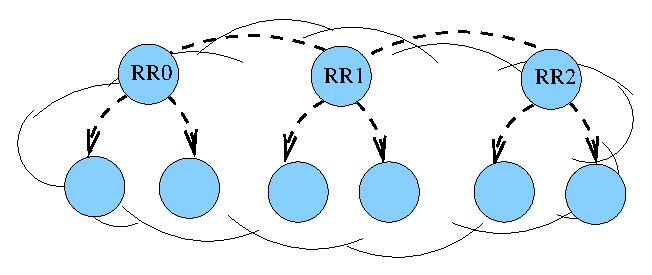
\includegraphics{rlogic/figures/path_vis_ibgp.eps}}
\end{psfrags}
\caption[The main idea of the proof of
  Theorem~\ref{thm:vis}.]{Illustrating the main idea of the proof of
  Theorem~\ref{thm:vis}.}
\label{fig:path_vis_ibgp}
\end{figure}

\begin{proof}
Call the set of routers that are not reflector clients the ``top layer''
of $\I$.  If the top layer is not a clique, then there are two routers
with no iBGP session between them, such that no route learned via eBGP
at $RR_i$ will ever be disseminated to $RR_j$, since no router
readvertises an iBGP-learned route (\eg, $RR_0$ and $RR_2$ in
Figure~\ref{fig:path_vis_ibgp}), and vice versa.  Furthermore, no route that
is learned via eBGP at any of $RR_i$'s clients will be disseminated to
$RR_j$ or $RR_j$'s clients, and vice versa.

Conversely, suppose the top layer is a clique. Observe that if a route
reflector has a route to the destination, then all of its clients have a
route as well.  Thus, if every router in the top layer has a route, all
routers in the AS will have a route.  If any router in the top layer
learns a route through eBGP, then all the top layer routers will hear of
the route (because the top layer is a clique).  Alternatively, if no
router at the top layer hears an eBGP-learned route, but some other
router in the AS does, then that route propagates up a chain of route
reflectors (each client sends it to its reflector, and the reflector
sends it on all its iBGP sessions) to the top layer, from there to all
the other top-layer routers, and from there to the other routers in the
AS.
\end{proof}

The results in this section suggest that path visibility can be
guaranteed by checking relatively simple constraints on the iBGP
topology, which can be determined by analyzing the static configuration
files alone.  Although, in the long term, architectural changes could be
made to guarantee that no configuration ever violates path
visibility~\cite{id-versatile-rr, caesar2004, feamster:fdna2004},
relatively simple checks against routing configuration can guarantee
path visibility today (as we will see in Chapter~\ref{chap:rcc}). 



\section{Safety}\label{sec:safety_def}

%In this section, we discuss properties related to improving
%predictability in Internet routing: {\em safety} and {\em determinism}.
Violations of safety can cause the routing protocol
to continually send routing updates that do not reflect changes in the
underlying topology.  We provide an informal definition of
safety and defer a formal definition to Chapter~\ref{chap:policy}
(Definition~\ref{def:safety}).

\begin{defn}[Safety]
A routing protocol satisfies {\em safety} if and only if, given no
changes to available paths after time $t_0$, then, at some finite time
$t_s > t_0$, each node $v\in G$ selects some route $r$ and does not
select a route $r'\neq r$ for any $t > t_s$.
\end{defn}

Safety is an important property because it guarantees that changes in
{\em routes} (\ie, routing update messages) correspond directly to
changes in available {\em paths}.  This invariant is important for
several reasons.  First, if the routing protocol causes routers to
change routes unnecessarily (\ie, when the paths are in fact stable),
the protocol itself may cause performance degradations, such as lost or
reordered packets.  Second, if routing changes do not correspond to
changes in the actual topology, then debugging the cause of an
oscillation becomes more difficult, because an operator cannot determine
whether routing changes reflect problems with infrastructure (\eg, flaky
or failing equipment) or the routing protocol itself.

Safety problems arise for two reasons:
\begin{enumerate}
\itemsep=-1pt
\item Conflicting route selections within the same AS, caused by
  interactions between BGP route attributes and the IGP (iBGP safety).
\item Conflicting rankings, caused by conflicting policies between
  ASes (eBGP safety).
\end{enumerate}
In both cases, guaranteeing safety is hard.  The
rest of this section focuses on the constraints for guaranteeing safety
in iBGP.  Guaranteeing that eBGP satisfies safety requires either 
knowing the rankings of ASes across the {\em global} Internet (not
a realistic requirement, because ASes typically insist on keeping their
rankings private) or placing restrictions on how each AS can specify
rankings and filters.  This problem is the focus of
Chapter~\ref{chap:policy}.

Safety violations in iBGP occur because BGP's route selection process
(as described in Table~\ref{tab:background:decision},
Section~\ref{sec:bg:route_selection}) does 
not satisfy {\em determinism}.  Determinism essentially says that the
route each router ultimately selects should not depend on either 
(1)~the presence or absence of routes
that would not be selected in the first place or
(2)~the
order in which messages arrive.  We formally define
determinism and explain why guaranteeing this property is difficult in
practice.
\begin{defn}[Selection function]
A selection function at router $r$, $\lambda_r$, takes as input a set of
routes $R_d = \{r_1, \ldots, r_n\}$ for some destination $d$ and produces
a single route $r_i \in R_d$.  The route $r_i$ is often called the
router's ``best route'' to $d$.
\end{defn}

\begin{defn}[Determinism]\label{def:determinism}
A routing protocol satisfies {\em determinism} for destination $d$ if,
for all routers $r$, if $r$ has a set of routes $R_d$ to $d$,
$\lambda_r(R_d)$ satisfies the following two properties:
\begin{enumerate}
\itemsep=-1pt
\item $\lambda_r(R_d) = \lambda_r(R'_d)$, where $R'_d$ is any subset of
  $R_d$ that contains $\lambda_r(R_d)$, and
\item $\lambda_r(R_d)$ does not depend on the order in which the routes
  in $R_d$ arrived at router $r$.
\end{enumerate}
Determinism depends only on the
selection function, $\lambda_r$, for all routers $r$.  Thus, we may also
discuss a single selection function, $\lambda_r$, in terms of whether it
satisfies determinism.
%% Let $\Sigma(R_d) = \{\sigma_1(R_d), \ldots, \sigma_{n!}(R_d)\}$ as
%% the set of all permutations of $R_d$ (\ie, the set of all possible
%% arrival orders for the candidate routes to $r_d$.
%% %
%% Let $T(R_d) = \{t_1(R_d), \ldots, t_{2^n}(R_d)\}$ be the set of all
%% subsets of $R_d$. 
%% %
%% Then, determinism is satisfied if and only if, for all $r_i \in
%% R_d$, $\lambda_r(R_d) = r_i \Rightarrow (r_i \in t_i(R_d) \Rightarrow
%% \lambda_r(\sigma_i(t_i(R_d))) = r_i)$, for all $\sigma_i \in \Sigma(R_d),
%% t_i \in T(R_d)$.
\end{defn}

%% In other words, if a router $r$ selects a certain route as its best
%% route from a set of candidate routes, then it should {\em always} select
%% that route if other routes are removed from that candidate set, and it
%% should always select that route regardless of the order in which
%% those routes arrive at router $r$.
Determinism is important for predictability; moreover, as the following
observation shows, violations of determinism can induce safety
violations, even when the selection function of only one router violates
determinism.


\begin{figure}
\centering
\begin{psfrags}
\psfrag{R1}{{\Large $R_1$}}
\psfrag{R2}{{\Large $R_2$}}
\psfrag{1}{$1$}
\psfrag{2}{$2$}
\psfrag{A}{$A$}
\psfrag{B}{$B$}
\psfrag{C}{$C$}
\psfrag{r1}{$\lambda_{R_1}(\{A,B\}) = A$; $\lambda_{R_1}(\{A,C\}) = C$}
\psfrag{r2}{$\lambda_{R_2}(\{A,B, C\}) = C$;  $\lambda_{R_2}(\{B,C\}) = B$}
\psfrag{A/P}{$A/\phi$}
\psfrag{B/C}{$B/C$}
%
\hspace{-0.4in}
\resizebox{0.7\textwidth}{!}{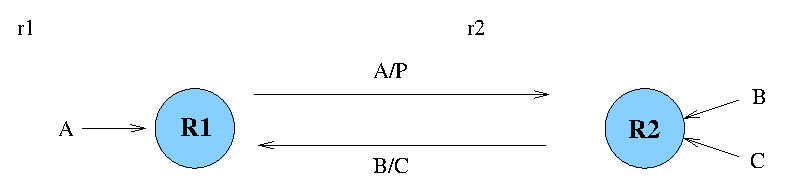
\includegraphics{rlogic/figures/det_a.eps}}
\end{psfrags}
%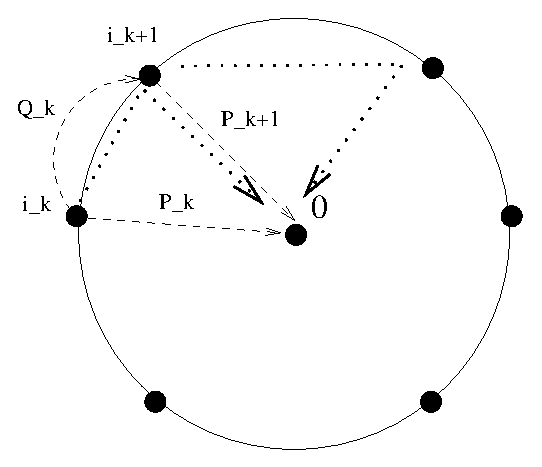
\epsfig{file=policy/figures/dw.eps,width=0.28\textwidth}
\caption[How determinism violations can cause safety
  violations.]{$\lambda_{R_2}$ does not satisfy determinism.  This violation
  can causes a safety violation.}
\label{fig:determinism}
\end{figure}


\begin{figure}
\centering
\begin{psfrags}
\psfrag{R1}{{\Large $R_1$}}
\psfrag{R2}{{\Large $R_2$}}
\psfrag{R3}{{\Large $R_3$}}
\psfrag{1}{$1$}
\psfrag{2}{$2$}
\psfrag{3}{$3$}
\psfrag{A}{$A$}
\psfrag{B}{$B$}
\psfrag{C}{$C$}
\psfrag{r1}{$\lambda_{R_1}(\{A,C\}) = C$;  $\lambda_{R_1}(\{A,B\}) = A$}
\psfrag{r2}{$\lambda_{R_2}(\{A,B, C\}) = C$;  $\lambda_{R_2}(\{B,C\}) = B$}
\psfrag{A/P}{$A/\phi$}
\psfrag{B/C}{$B/C$}
%
\hspace{-1.5in}
\resizebox{0.7\textwidth}{!}{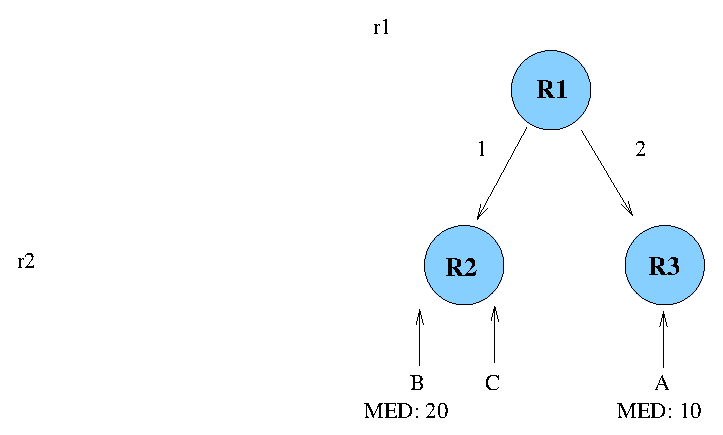
\includegraphics{rlogic/figures/det_b.eps}}
\end{psfrags}
%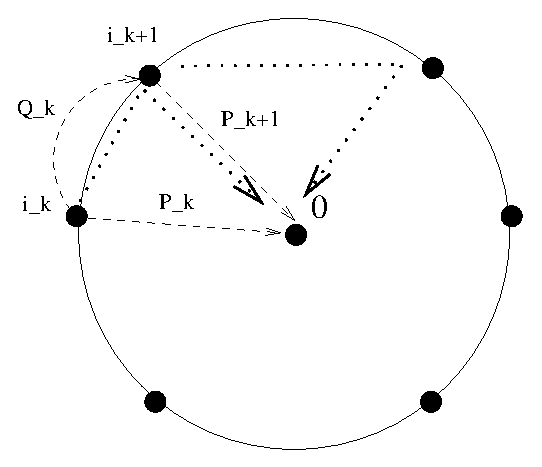
\epsfig{file=policy/figures/dw.eps,width=0.28\textwidth}
\caption[Instantiation of Figure~\ref{fig:determinism} in a BGP
  configuration.]{Instantiation of Figure~\ref{fig:determinism} in a BGP
  configuration.  Router $1$ is a route reflector with two clients, $R_2$
  and $R_3$.  Costs on edges are IGP path costs.  Router $R_2$ prefers route
  $B$ over route $C$ due to a tiebreak.}
\label{fig:determinism_bgp}
\end{figure}

\begin{observation}
If the selection function of even one router, $\lambda_r$, violates
determinism, then the routing protocol may also violate safety.
\end{observation}

\noindent
The following example illustrates this point.

\begin{example}\label{ex:med_det}
Consider Figure~\ref{fig:determinism}.  Router $R_1$ selects route $A$
given the choices $\{A, B\}$ and selects route $C$ given choices
$\{A,C\}$. This selection function satisfies determinism.
On the other hand, router $R_2$'s selection function violates determinism:
$\lambda_{R_2}(\{A,B,C\}) = C$, but $\lambda_{R_2}(\{B,C\}) = B$.  The
interaction of the two selection functions creates the following
oscillation: 
\begin{enumerate}
\itemsep=-1pt
\item Router $R_1$ receives only route $A$, selects it, and
  advertises this route to router $R_2$.
\item Router $R_2$ has received $\{A,B,C\}$, selects
  route $C$, and advertises it to router $R_1$.
\item Router $R_1$ has received $\{A,C\}$, selects
  route $C$, and sends a withdrawal ($\phi$) for route $A$ to router
  $R_2$. 
\item Router $R_2$ selects $B$ from the set $\{B,C\}$ and advertises it to
  router $R_1$, implicitly withdrawing route $C$. 
\item Router $R_1$ now has to select a route from the set $\{A,B\}$, selects
  route $A$, and advertises it to router $R_2$.
\end{enumerate}
This process repeats forever, violating safety.
\end{example}

\subsection{Determinism Violations in BGP: The MED Attribute}

It turns out that the above scenario can occur in BGP, because the MED
attribute causes each router's selection function to violate
determinism.  The addition of a third router, as shown in
Figure~\ref{fig:determinism_bgp}, gives rise to the oscillation from the
previous example.  In this case, router $R_1$ is a route reflector for
two clients: routers $R_2$ and $R_3$, with IGP costs as shown.  Routes
$A$ and $B$ are advertised by the same AS, and route $A$ has a lower MED
value (and, hence, is preferred to $B$).  In this setup, the selection
functions are exactly as described 
in the from Figure~\ref{fig:determinism}: when router $R_2$ learns $\{A,B,C\}$,
route $B$ is eliminated due to MED, and route $C$ is selected because it
is an eBGP-learned route.  When router $R_2$ learns only $\{B,C\}$, on
the other hand, it prefers route $B$ over route $C$ due to the router ID
tiebreak.  Similarly, router $R_1$ prefers route $C$ over route $A$ due
to IGP, but router $A$ over router $B$ due to MED.  The routing system
in this example oscillates in the same fashion as the one shown in
Figure~\ref{fig:determinism}. 

As the above example shows, the interaction between the MED attribute
and route reflection can cause BGP to violate safety.  Note that this
example satisfies the guidelines that were specifically proposed to
avoid these types of oscillations~\cite{rfc3345}.  Even though not all
safety violations are caused by violations of determinism, eliminating
BGP's determinism problem can eliminate all oscillations that do not
involve cyclic preferences over routes caused by setting the local
preference attribute.  Specifically, by making the MED attribute
comparable across {\em all} routes, rather than just those from the same
AS, each router's selection function can be made to satisfy determinism.
We now formally show this result.

\begin{lemma}\label{lem:det_med}
If a router's selection function compares the MED attribute across all
routes to a destination (rather than just across those from the same
neighboring AS), then its selection function satisfies determinism.
\end{lemma}

\begin{proof}
We must show that if the router's selection function compares the MED
attribute across all routes to a destination then: (1)~the route it
selects does not change when any route is removed from that set; and
(2)~the route it selects does not depend on the order in which the
router receives them.

When a router compares the MED attribute across all routes to a
destination, then all routes to a destination can be totally ordered.
Specifically, all routes can be sorted by local preference.  Each set of
routes with equal local preference can be sorted from shortest AS path
length to longest, and so forth.  Thus, the set of routes to a
destination can 
be totally ordered, and removing a route from that set that is not the
most preferred in the total ordering will not change the most preferred
route, since that route must have had a lower local preference, longer
AS path length, higher origin type, lower MED, etc.  

We must also show that the route a router $r$ selects, $\lambda_r(R_d)$,
does not depend on the order that $r$ receives the routes in $R_d$.
%Define two message arrival orders, $\sigma_i(R_d)$ and $\sigma_j(R_d)$,
%and suppose that $\lambda_r(\sigma_i(R_d)) = \rho_i \in R_d$, but
%$\lambda_r(\sigma_j(R_d)) = \rho_j \in R_d$, where $\rho_i \neq \rho_j$.
We know that the routes in $R_d$ are totally ordered, which means that
there is a preference relation between any two routes $\rho_i$ and
$\rho_j$ that is consistent for {\em any} subset of $R_d$ that contains
both $\rho_i$ and $\rho_j$.  We also know that $\lambda_r(R_d)$ will
ultimately select the route that is most preferred in that total
ordering.  Suppose that most preferred route is $\rho_i$.  When $\rho_i$
arrives, $r$ will select $\rho_i$ and continue to select it even after
other routes arrive.  Thus, if $\rho_j$ arrives before $\rho_i$, then
the router will not continue to select $\rho_j$ after $\rho_i$ arrives,
since $\rho_i$ is strictly better than $\rho_j$ in the total ordering.
Similarly, if $\rho_j$ arrives after $\rho_i$, then $r$ will continue to
select $\rho_i$, since it is better than $\rho_j$ in the total ordering.
\end{proof}

We explore how comparing the MED attribute across all routes affects
protocol operation, as well as how this might be done in practice, in
Section~\ref{sec:sandbox:med_disc}.  In short, the primary benefit of
making the route selection function deterministic is that a set of
routers {\em 
within a single AS} may violate safety if determinism is not
satisfied.  Although determinism prevents safety violations such as
those shown in Figures~\ref{fig:determinism}
and~\ref{fig:determinism_bgp}, it does not prevent {\em all} violations
of safety.  For that, we require a stronger notion of determinism, which
we call {\em egress determinism}.


\subsection{Egress Determinism Violations in BGP: Route Reflection}

Even if determinism is satisfied, an AS's iBGP topology can still cause
a routing protocol to violate
safety.  In particular, we can construct an oscillation that
involves the interaction between an AS's route reflector topology and
its IGP topology.  To better understand this interaction, we first
define the notion of {\em egress determinism}.  Egress determinism is a
stronger condition than determinism, as shown in
Figure~\ref{fig:determinism_venn}; essentially, it states that, given a
set of routes learned at {\em any} egress router in the AS, a router's
preference between any pair of those routes should not depend on either
the order in which those routes arrive or the presence or absence of
other routes.  Egress determinism implies determinism, but it also
states that every router's selection function should satisfy determinism
for all routes learned at {\em any} router in the AS, not just those
learned locally at that router.

\begin{figure}
\centering
\begin{psfrags}
\resizebox{0.4\textwidth}{!}{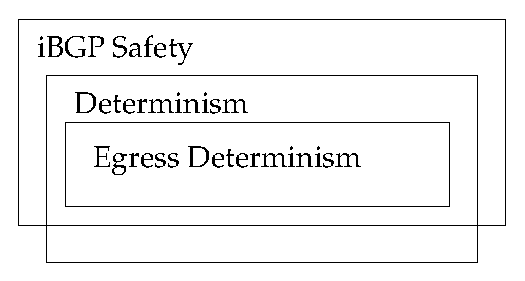
\includegraphics{rlogic/figures/det_venn.eps}}
\end{psfrags}
%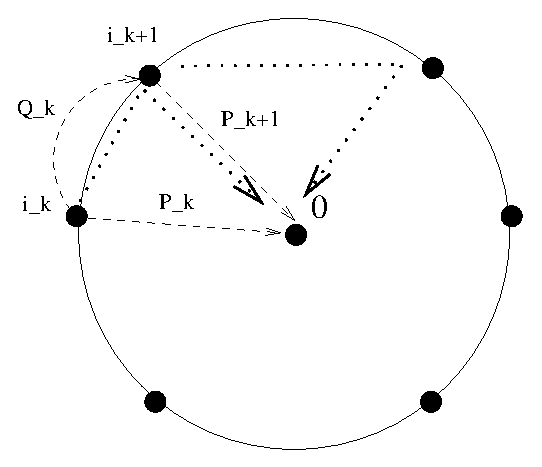
\epsfig{file=policy/figures/dw.eps,width=0.28\textwidth}
\caption[The relationship between determinism, egress determinism, and
  safety.]{The relationship between determinism, egress determinism, and
  safety.} 
\label{fig:determinism_venn}
\end{figure}


\begin{defn}[Egress Determinism]\label{def:egress_determinism}
Let $E_d$ be the set of routes for destination $d$ learned at {\em any}
router in the AS.  Then, a routing protocol satisfies {\em egress
determinism} for destination $d$ if $\lambda_r(E_d)$ satisfies the
following two properties:
\begin{enumerate}
\itemsep=-1pt
\item $\lambda_r(E_d) = \lambda_r(E'_d)$, where $E'_d$ is any subset of
  $E_d$ that contains $\lambda_r(E_d)$, and
\item $\lambda_r(E_d)$ does not depend on the order in which the routes
  in $E_d$ arrived at router $r$.
\end{enumerate}
\end{defn}

\begin{figure}
\centering
\begin{psfrags}
%
\psfrag{x}{{\LARGE $x$}}
\psfrag{y}{{\LARGE$y$}}
\psfrag{z}{{\LARGE $z$}}
\psfrag{X}{{\LARGE $X$}}
\psfrag{Y}{{\LARGE $Y$}}
\psfrag{Z}{{\LARGE $Z$}}
\psfrag{R1}{{\LARGE $R_1$}}
\psfrag{R2}{{\LARGE $R_2$}}
%
%\hspace{-0.7in}
\resizebox{0.6\textwidth}{!}{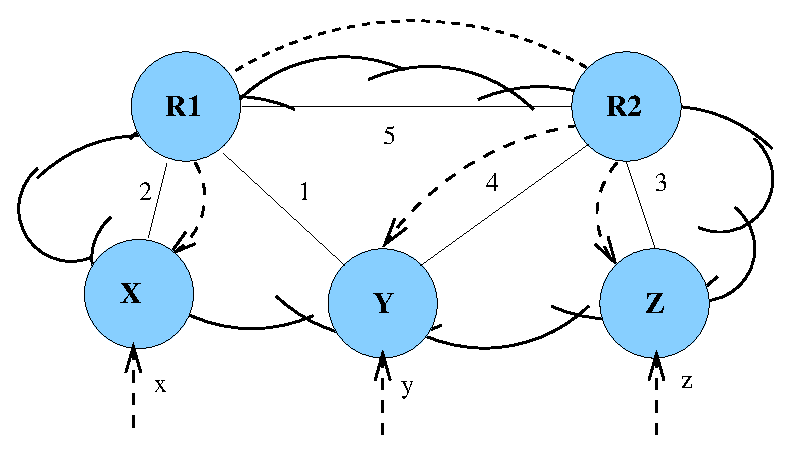
\includegraphics{rlogic/figures/det_violation_rr.eps}}
\end{psfrags}
%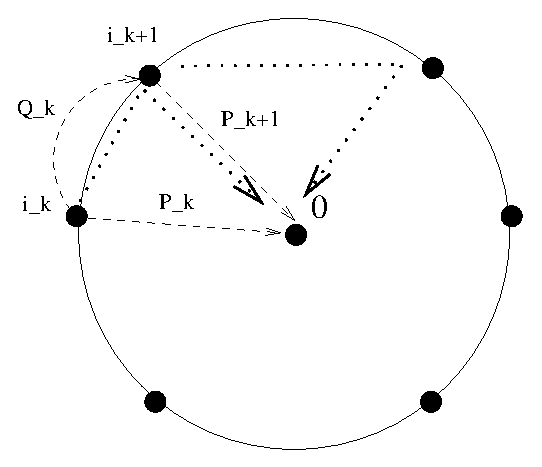
\epsfig{file=policy/figures/dw.eps,width=0.28\textwidth}
\caption[The interaction of IGP and iBGP can cause a violation of egress
  determinism.]{The interaction of IGP and iBGP can cause a violation of egress
  determinism. $\lambda_{R_1}$ is equal to either $x$ or $y$ depending
  on whether $z \in E_d$.}
\label{fig:det_violation_rr}
\end{figure}

Note that egress determinism is a stronger condition than determinism
because it states
properties that $\lambda_r$ must satisfy over the set of routes learned
by all routers in the AS, not just the routes learned at $r$.

If every router in the AS always learned all routes in $E_d$, then
violations of egress determinism would never cause oscillations: given a
fixed set of routes $E_d$, every router would always see that set and
select the same route.  In an iBGP topology with route reflectors,
however, most routers will see some subset of $E_d$, which means that
violations of egress determinism may cause safety violations.  Consider
Figure~\ref{fig:det_violation_rr}: $X$ is a route reflector client of
$R_1$, and $Y$ and $Z$ are clients of route reflector $R_2$. Suppose
that routers $X$, $Y$, and $Z$ all learn routes for some destination $d$
with equal local preference, AS path length, origin type, and MED
attributes, causing routers within the pictured AS to resort to
preferring eBGP routes over iBGP routes, and, that being equal, to
prefer routes with the shortest IGP path cost.  If $E_d = \{x,y,z\}$,
then $\lambda_{R_1}(E_d) = x$: $R_2$ selects $z$ due to its shorter IGP
path cost to the next hop, and $R_1$, having learned $x$ and $z$,
selects route $x$.  If, on the other hand, $E_d = \{x,y\}$, then
$\lambda_{R_1}(E_d) = y$: $R_2$ selects $y$, and $R_1$, having learned
both $x$ and $y$, selects $y$ due to the shorter IGP path cost. Thus,
the first condition of egress determinism is violated.

\begin{figure}
\centering
\begin{psfrags}
%
\psfrag{R1}{{\LARGE $R_1$}}
\psfrag{R2}{{\LARGE $R_2$}}
\psfrag{R3}{{\LARGE $R_3$}}
\psfrag{x}{{\LARGE $x$}}
\psfrag{y}{{\LARGE $y$}}
\psfrag{z}{{\LARGE $z$}}
\psfrag{r1}{{\LARGE $\lambda_{R_1}(\{x,y\}) = y$;
    $\lambda_{R_1}(\{x,y,z\}) = x$}}
\psfrag{r2}{{\LARGE $\lambda_{R_2}(\{x,z\}) = z$;
    $\lambda_{R_2}(\{x,y,z\}) = x$}} 
\psfrag{r3}{{\LARGE $\lambda_{R_3}(\{y,z\}) = z$;
    $\lambda_{R_3}(\{x,y,z\}) = y$}}
\psfrag{x/y}{{\LARGE $x/y$}}
\psfrag{y/z}{{\LARGE $y/z$}}
\psfrag{x/z}{{\LARGE $x/z$}}
%
\hspace{-0.7in}
\resizebox{0.85\textwidth}{!}{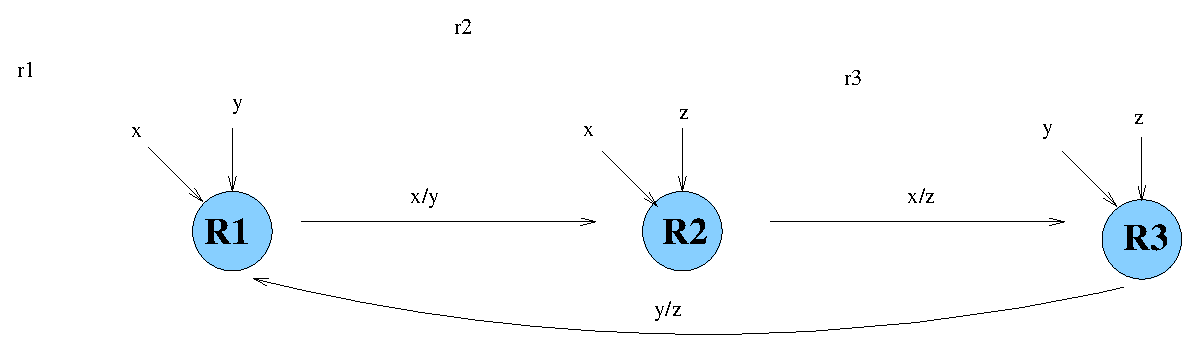
\includegraphics{rlogic/figures/abstract_sd.eps}}

\end{psfrags}
%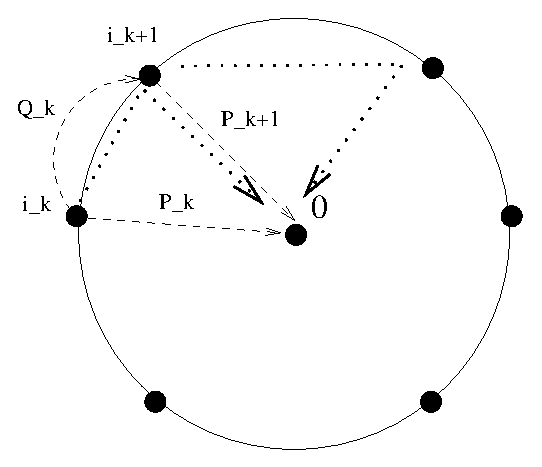
\epsfig{file=policy/figures/dw.eps,width=0.28\textwidth}
\caption[Egress determinism violations can cause safety
  violations.]{Violations of egress determinism can also cause the
  routing protocol to violate safety.}
\label{fig:abstract_sd}
\end{figure}


Like determinism violations, egress determinism violations can cause the
routing protocol to violate safety.  Consider three routers whose
selection functions violate egress determinism, as shown in
Figure~\ref{fig:abstract_sd}; $R_1$'s selection function is identical to
that in Figure~\ref{fig:det_violation_rr}. Each router prefers one route
or the other depending on the presence or absence of a third route.  In
this case, there is no stable assignment of routes $x$, $y$, and $z$ to
routers $R_1$, $R_2$, and $R_3$.  For example, if $R_1$ selects $x$,
then $R_2$ selects $z$ and $R_3$ selects $y$, prompting $R_1$ to select
$y$, and so on.  This very scenario can be realized in BGP today if
three routers' route selection functions fail to satisfy egress
determinism, as shown in Figure~\ref{fig:sd_violation_rr_osc}.


\begin{figure}[t]
\centering
\begin{psfrags}
%
\psfrag{x}{{\LARGE $x$}}
\psfrag{y}{{\LARGE$y$}}
\psfrag{z}{{\LARGE $z$}}
\psfrag{X}{{\LARGE $X$}}
\psfrag{Y}{{\LARGE $Y$}}
\psfrag{Z}{{\LARGE $Z$}}
\psfrag{R1}{{\LARGE $R_1$}}
\psfrag{R2}{{\LARGE $R_2$}}
\psfrag{R3}{{\LARGE $R_3$}}
%
%\hspace{-0.7in}
\resizebox{0.6\textwidth}{!}{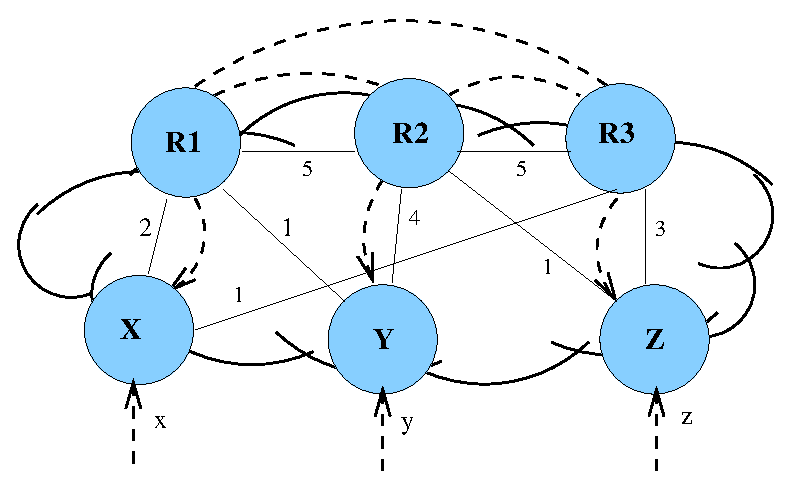
\includegraphics{rlogic/figures/sd_violation_rr_osc.eps}} 

\end{psfrags}
%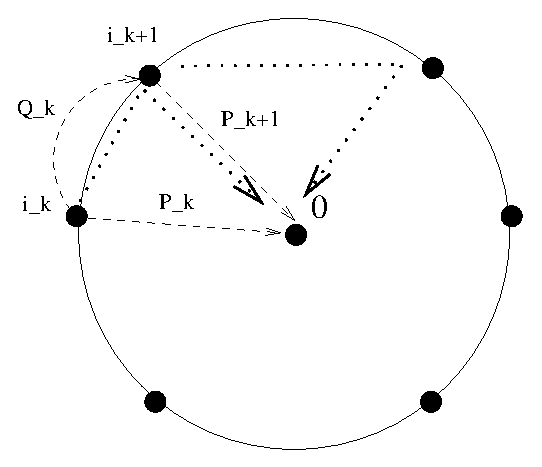
\epsfig{file=policy/figures/dw.eps,width=0.28\textwidth}
\caption[The interaction of IGP and iBGP can cause a violation of egress
  determinism.]{The interaction of IGP and iBGP can cause a violation of egress
  determinism that induces a safety violation.  This figure shows the
  instantiation of Figure~\ref{fig:abstract_sd} in BGP.  Previous work has
  also observed that violations of this type could occur~\cite{Griffin2002}
  but did not observe that these could be constructed in general by
  composing egress determinism violations.}
\label{fig:sd_violation_rr_osc}
\end{figure}


\begin{figure}
\begin{center}
\begin{psfrags}
\psfrag{R1}{{\LARGE $R_1$}}
\psfrag{R2}{{\LARGE $R_2$}}
\psfrag{X}{{\LARGE $X$}}
\psfrag{Y}{{\LARGE $Y$}}
\psfrag{Z}{{\LARGE $Z$}}
\psfrag{x}{{\Large $x$}}
\psfrag{y}{{\Large $y$}}
\psfrag{z}{{\Large $z$}}
\psfrag{l1}{{\Large $l_r$}}
\psfrag{ly}{{\Large $l_y$}}
\psfrag{lx}{{\Large $l_x$}}
\psfrag{lz}{{\Large $l_z$}}
\resizebox{0.45\textwidth}{!}{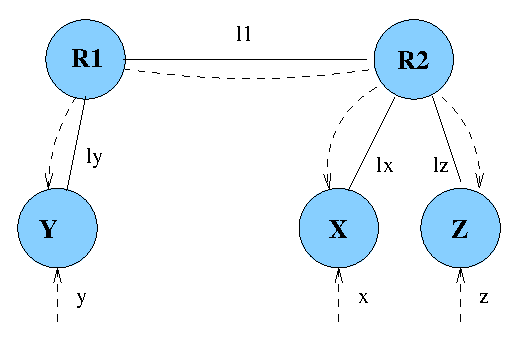
\includegraphics{rlogic/figures/det_igp.eps}}
\end{psfrags}
\end{center}
\caption[The main idea of the proof of
  Lemma~\ref{lem:det_igp}.  ]{The main idea of the proof of
  Lemma~\ref{lem:det_igp}.  
%
If $R_2$ prefers $z$ over $x$, then $l_z \leq l_x$.
%
If $R_1$ prefers $x$, given routes $x$, $y$, and $z$, then $l_y \geq
  l_r + l_x$.  If $R_2$ is on the shortest IGP path between $R_1$ and
  both $X$ and $Z$, it follows that $l_y \geq l_r + l_z$ (and, hence,
  $R_1$ would {\em not} have selected route $y$).  Thus, for $R_1$ to
  prefer route $y$ when it learns routes $x$ and $z$, its shortest path
  to either egress router $Y$ or $Z$ must not traverse $R_2$. (The links
  labeled with $l_x$, $l_y$, and $l_z$ are shown as single IGP links,
  but the argument generalizes to IGP paths.)}
\label{fig:det_igp}
\end{figure}



\begin{lemma}\label{lem:det_igp}
If an AS's iBGP topology is {\em RR-IGP-Consistent}, and every router's
selection function satisfies determinism, then every router's selection
function also satisfies egress determinism.
\end{lemma}

\begin{proof}
Suppose that there exists some router $R_1$ and routes $x$, $y$, and $z$
(not necessarily learned via eBGP at $R_1$) such that
$\lambda_{R_1}(\{x,y,z\}) = y$, but $\lambda_{R_1}(\{x,y\}) = x$.  
%
First, because $\lambda_{R_1}$ satisfies determinism, it must be the case
that (1)~$R_1$ learns $x$ via iBGP and (2)~some router $R_2$ in the iBGP
topology withdraws the eBGP-learned 
route $x$ from router $R_1$ upon learning the route $z$, thereby
preventing router $R_1$ from receiving route $x$ (if $R_1$ had learned
$x$ directly via eBGP, it would continue to select route $x$).
%
Second, $R_2$ must have selected $z$ over $x$ because it had a shorter
IGP path to the router from which it learned $z$---if $x$ had been less
desirable based on some other attribute (\eg, AS path length), then $r$
would have also selected the route $z$ upon learning it from $R_2$,
rather than selecting $y$ instead.
%
Third, because $R_1$ selects $y$ after learning $z$ from $R_2$, its IGP
path to the egress router that learned $y$ must be shorter than its IGP
path to the router that learned $z$, yet longer than its IGP path to the
router that learned $x$.   
%
This relation among distances to egresses is only possible if the
shortest path between $R_1$ and either the egress router that learned
route $x$ or $z$ does not traverse $R_2$ (\ie, the iBGP topology is not
{\em RR-IGP-Consistent}).  Figure~\ref{fig:det_igp} shows why this
relation is not possible in an iBGP topology that is {\em
RR-IGP-Consistent}.
\end{proof}

We now state the conditions for iBGP to satisfy safety using our results
involving determinism and egress determinism.  Specifically, we show
that if MED is compared across all routes (\ie, every router's selection
function satisfies determinism) and if the iBGP topology is {\em
RR-IGP-Consistent} (\ie, egress determinism is satisfied), then iBGP
satisfies safety.

\begin{figure}
\begin{center}
\begin{psfrags}
\psfrag{R1}{{\LARGE $R_1$}}
\psfrag{R2}{{\LARGE $R_2$}}
\psfrag{C1}{{\LARGE $C_1$}}
\psfrag{C2}{{\LARGE $C_2$}}
\resizebox{0.55\textwidth}{!}{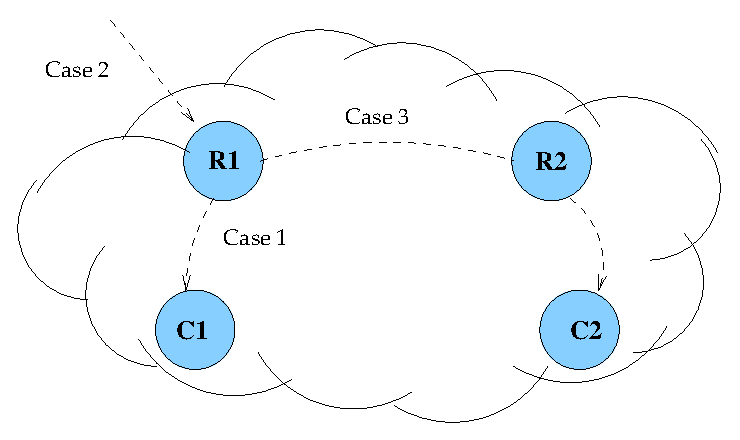
\includegraphics{rlogic/figures/always_compare.eps}} 
\end{psfrags}
\end{center}
\caption[The three cases in the proof of
  Theorem~\ref{th:always_compare}.]{The three cases in the proof of
  Theorem~\ref{th:always_compare}.}
\label{fig:always_compare}
\end{figure}



\begin{theorem}\label{th:always_compare}
If every router's selection function compares MED attribute across all
routes and the iBGP topology is {\em RR-IGP-Consistent}, then iBGP
satisfies safety.
\end{theorem}

\begin{proof}
The proof follows from Lemmas~\ref{lem:det_med} and~\ref{lem:det_igp}.
If the conditions of the theorem hold, then BGP satisfies both
determinism and egress determinism.  It remains to show that no iBGP
topology can violate safety if it satisfies both determinism and egress
determinism.  

We must show that, for any route that a router ultimately selects, other
routers in the AS will not select routes that ultimately causes the
original router to change the route it selects.  For simplicity, we will
consider an iBGP route reflector hierarchy with one level.  The argument
can be extended to a multiple-level hierarchy, and to a network with
multiple top-level routers or multiple clients per route reflector,
without loss of generality.  Consider the possible propagation of BGP
routes between routers $C_1$ and $C_2$ and their route reflectors $R_1$
and $R_2$, as shown in Figure~\ref{fig:always_compare}.  Suppose $C_1$
and $C_2$ initially select routes via eBGP; each will readvertise these
routes to $R_1$ and $R_2$.  Then, there are three cases:

\begin{enumerate}
\itemsep=-1pt
\item {\em $R_1$ prefers the route through its client $C_1$.}
In this case, $R_1$'s selection of the route through $C_1$ will
obviously not cause either $R_1$ or $C_1$ to switch paths.  
%
\item {\em $R_1$ prefers its own eBGP-learned route (analogously for
$R_2$).}  In this case, $C_1$ learns a route via $R_1$. If it
continues to prefer its own route, neither router will select a new
route. If, on the other hand, it prefers the route through $R_1$, then
it will withdraw its eBGP-learned route from $R_1$.  However, since
$\lambda_{R_1}$ satisfies determinism, $R_1$ will continue to select its
own eBGP-learned route when it receives this withdrawal.
%
\item {\em $R_1$ prefers a route via $R_2$ or $C_2$ (analogously for
$R_2$).}  A similar argument can be used to show that
neither $R_1$ nor $C_1$ will select a new route once $R_1$ selects a
route via $C_1$.  For the third case, we must also show that $R_1$'s
withdrawal of either its own route or the route via $C_1$ from $R_2$
will cause neither $R_2$ nor $C_2$ to change routes.  Since $R_1$
prefers a route via $R_2$ then $R_2$ selected its own route
or the route via $C_2$; egress determinism guarantees that $R_1$'s
withdrawal will not cause either $C_2$ or $R_2$ to change its route
selection.
\end{enumerate}
\end{proof}

Our definitions have allowed us to derive sufficient
conditions on safety that are significantly weaker (and therefore, the
result is stronger) than in
previous work~\cite{Griffin2000}.  In particular, {\em our results show
that assuming that the relationships between route reflectors and their
clients are acyclic is unnecessary} (although a cyclic topology may make
an oscillation more likely if egress determinism is
violated).  It turns out that the only way for a cyclic iBGP topology
to cause oscillations would be for either the iBGP topology to not be
{\em RR-IGP-Consistent} or for some IGP edges to have
negative edge weights.

\begin{figure}
\centering
\begin{psfrags}
%
\psfrag{x}{{\LARGE $x$}}
\psfrag{y}{{\LARGE$y$}}
\psfrag{z}{{\LARGE $z$}}
\psfrag{X}{{\LARGE $X$}}
\psfrag{Y}{{\LARGE $Y$}}
\psfrag{Z}{{\LARGE $Z$}}
\psfrag{R1}{{\LARGE $R_1$}}
\psfrag{R2}{{\LARGE $R_2$}}
\psfrag{R3}{{\LARGE $R_3$}}
\psfrag{l1}{{\LARGE $l_1$}}
\psfrag{l2}{{\LARGE $l_2$}}
\psfrag{l3}{{\LARGE $l_3$}}
\psfrag{l4}{{\LARGE $l_4$}}
\psfrag{l5}{{\LARGE $l_5$}}
\psfrag{l6}{{\LARGE $l_6$}}
%
%\hspace{-0.7in}
\resizebox{0.7\textwidth}{!}{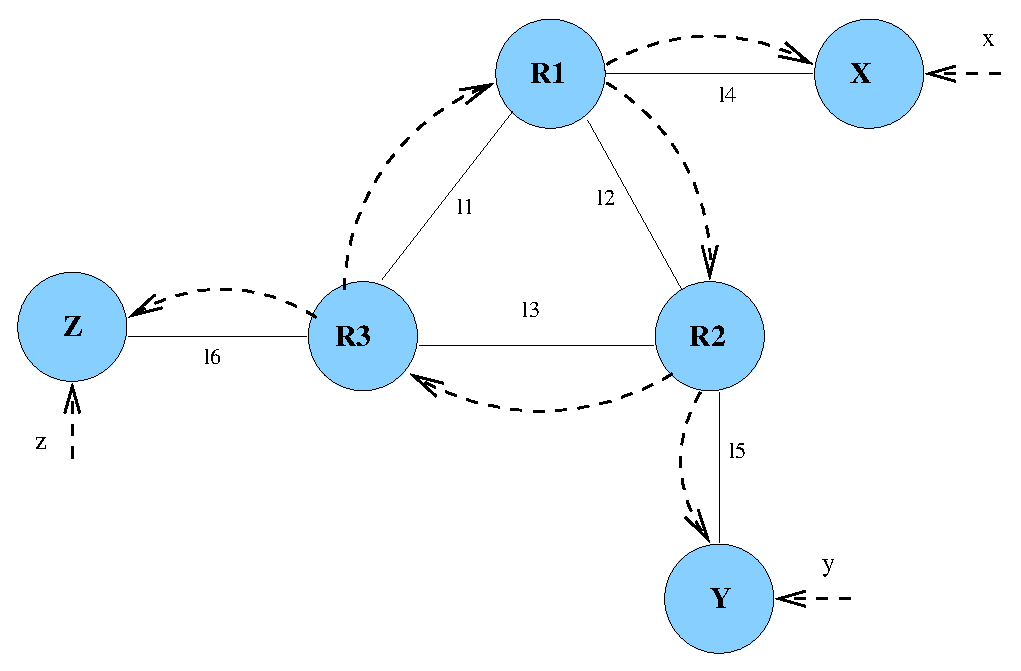
\includegraphics{rlogic/figures/ibgp_cycle.eps}} 

\end{psfrags}
%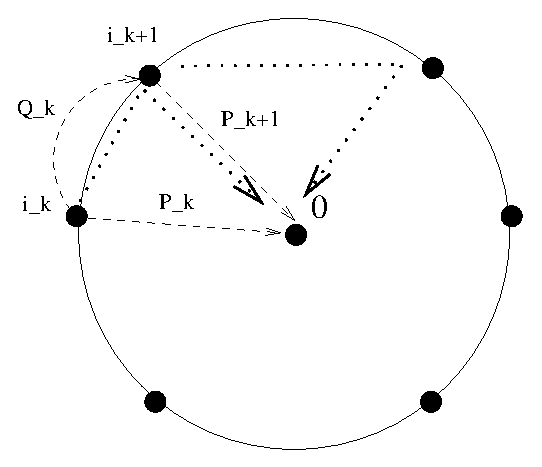
\epsfig{file=policy/figures/dw.eps,width=0.28\textwidth}
\caption[When iBGP satisfies egress determinism,
  a cyclic iBGP topology typically do not cause safety violations.]{When iBGP
  violates safety but satisfies egress determinism, the only way a
  cyclic iBGP topology can 
  violate safety is if the IGP allows negative edge weights.  This
  example shows an iBGP hierarchy that includes only six routers, but it
  generalizes: $R_i$ could be any cyclic relationship at the top of the
  hierarchy, $X$ could be a path through a sequence of iBGP sessions to
  the egress router $X$ (\eg, a sequence of route reflector-client
  sessions) and $l_4$ could be the cost of that path, and so forth.}
\label{fig:ibgp_cycle}
\end{figure}



To understand why cycles in the iBGP hierarchy do not cause problems if
the topology is {\em 
RR-IGP-Consistent}, see Figure~\ref{fig:ibgp_cycle}.  In this example,
if egress determinism is satisfied, then the only case where an
oscillation might result is where $R_1$ prefers route $y$ over route
$x$, $R_2$ prefers route $z$ over $y$, and $R_3$ prefers $x$ over $z$.
All other cases where oscillation might occur (\ie, those caused by
violations of egress determinism) require some shortest IGP path between
a router and another egress to not traverse that router's route reflector.
For safety to be violated in this example, routes $x$, $y$, and $z$ must
all have equal local preference, AS path length, origin type and MED
(otherwise, all routers would select the most preferable route or
routes).  Presuming that all routes are equally good up to the step in
route selection involving the IGP tiebreak, then the only way for such a
situation to occur is if the following inequalities were satisfied:
\begin{eqnarray*}
l_1 + l_4 & < & l_6 \\
l_2 + l_5 & < & l_4 \\
l_3 + l_6 & < & l_5 
\end{eqnarray*}
which implies that $l_1 + l_2 + l_3 < 0$, or that some IGP edge weights
must be negative.

Theorem~\ref{th:always_compare} is significant because
the conditions on the iBGP topology that are required to guarantee
safety are identical those for guaranteeing route validity, as stated in
Theorem~\ref{th:rr_safe}.  Furthermore, because there are now known
techniques for {\em generating} these
configurations~\cite{Vutukuru2005}, our results are prescriptive, since
this technique that was designed to generate iBGP topologies that
guarantee route validity also happens to generate topologies that
guarantee safety.

This section has described safety violations that result from
protocol interactions {\em within a single AS}.  However, safety is a somewhat
unique property because it inherently depends on how different ASes are
allowed to rank candidate routes to a destination (\ie,
Observation~\ref{obs:composable} is not satisfied).  Whereas, in iBGP, a
router's rankings are constrained by the underlying IGP
topology, in eBGP, an AS's rankings can be arbitrary.
Verifying a property that involves analyzing the interactions
between the configurations of multiple ASes is challenging:
because these ASes compete with one another, no single AS has knowledge 
of the configurations of other ASes.  Chapter~\ref{chap:policy} explores
how safety can be guaranteed {\em across multiple ASes} without
requiring each AS to expose its configurations to other ASes.


\section{Summary}

Detecting problems in Internet routing requires a precise
specification of correct behavior and a framework for reasoning about
whether that specification is satisfied.  In this chapter, we presented
a three-part correctness specification: route validity, path visibility,
and safety. We explained why each of these properties is important for the
fundamental operation of Internet routing and reasoned about how these
properties may be satisfied or violated in the context of BGP.

In the subsequent chapters of this dissertation, we will use the
specification constraints to guide the operations and design of correct
Internet routing.  In Chapter~\ref{chap:rcc}, we will explore how static
configuration analysis can be used to guarantee that two of these
properties---route validity and path
visibility---hold. 
Theorems~\ref{th:mesh}--\ref{thm:vis}
%, \ref{th:rr_safe},
%\ref{th:mesh_visibility}
%, and~\ref{thm:vis} 
suggest invariants on
configuration that could be verified by detecting when the configuration
violates certain invariants, and both Theorem~\ref{th:always_compare}
and the discussion at the end of
Section~\ref{sec:mesh}
suggest possible protocol modifications.  In
Chapter~\ref{chap:sandbox}, we will exploit the fact that, when the
routing protocol satisfies certain aspects of this specification
(specifically, path visibility, safety, and, in some cases,
determinism), we can design algorithms that efficiently predict the
routes that each router in an AS will ultimately select.
Chapter~\ref{chap:policy} tackles the problem of guaranteeing safety in
the context of eBGP, which is challenging since it inherently involves
dependencies between the policies of multiple independent (and often
competing) ASes.
%Chapter~\ref{chap:beyond} explores how both analysis of
%routing protocol dynamics and modifications to the routing architecture
%itself can complement static configuration analysis.





\qchapter{\textit{Things could be worse. \\  Suppose your errors were
    counted and published every day, \\ like those of a baseball player.}
    \vskip 0.1em  - Unknown}{\rccns: Detecting BGP Configuration Faults with Static
  Analysis}\label{chap:rcc} 

%\section{Introduction}

\cs{T}his chapter describes the design, implementation, and evaluation of
\textbf{\rccns},
the router configuration checker, a tool
that uses static analysis to detect faults in Border Gateway Protocol
(BGP) 
configuration.  
By finding faults over a
distributed set of router configurations, \rcc enables network
operators to test and debug configurations before deploying them in an
operational network. This approach improves on the status quo of
``stimulus-response'' debugging where operators need to run
configurations in an operational network before finding faults.

As described in Chapter~\ref{chap:related} (Section~\ref{sec:conf}),
network operators use router configurations to provide reachability,
express routing policy (\eg, transit and peering
relationships~\cite{Norton2000}, inbound and outbound
routes~\cite{Beijnum2002}, etc.), configure primary and backup
links~\cite{Gao2001b}, and perform traffic engineering across multiple
links~\cite{Feamster2004}.  The complex process of configuring routers
is exacerbated by the number of lines of code, by configuration being
distributed across the routers in the network, by the absence of useful
high-level primitives in today's configuration languages, by the
diversity in vendor-specific configuration languages, and by the number
of ways in which the same high-level functionality can be expressed in a
configuration language.  

Router configuration gives network operators the flexibility to control
traffic and implement complex business relationships, but its complexity
also means that router configurations are prone to
faults~\cite{Beijnum2002,Mahajan2002}.  Configuration faults include
invalid routes (including hijacked and leaked routes); contract
violations~\cite{Feamster2004b}; unstable routes~\cite{labovitz:ton01};
routing loops~\cite{Dube99,Feamster2003b}; and persistently oscillating
routes~\cite{Basu2002,Griffin99,Varadhan2000}.
%Section~\ref{s:nanogproblems} discusses the problems observed in
%operational networks in detail.  
As summarized in
Table~\ref{tab:empirical_results} (Section~\ref{sec:rcc_related}), BGP
configuration faults can seriously affect end-to-end Internet
connectivity, leading to lost packets, forwarding loops, and unintended
paths between hosts or ASes.  


\begin{figure}[t]
\begin{center}
%\resizebox{0.8\columnwidth}{!}{\includegraphics*[viewport=100 200 500 650]{rcc/figures/nanog_table.pdf}}
\centering\epsfig{file=rcc/figures/nanog_table.eps, angle=270, width=\linewidth}
\end{center}
\caption{Number of threads discussing routing
  faults on the NANOG mailing list.
}
\label{tab:nanogerrors}
\end{figure}


%% Chapter~\ref{chap:related} (Section~\ref{sec:configuration})
%% describes how BGP's configuration affects which routes are originated
%% and propagated, how routes are modified as they propagate, which route
%% each router selects from multiple options, and how routes propagate
%% between routers.  
To understand the extent to which this complex configuration is
responsible for the types of failures that occur in practice, we studied
the archives of the North American Network Operators Group (NANOG)
mailing list, where network operators report operational problems,
discuss operational issues, etc.~\cite{nanog-list}.  Because the list
has received about 75,000 emails over the course of ten years, we first
clustered the emails by thread and pruned threads based on a list of
about fifteen keywords (\eg, ``BGP'', ``issue'', ``loop'', ``problem'',
``outage'').  We then reviewed these threads and classified each of them
into one or more of the categories shown in
Figure~\ref{tab:nanogerrors}.  This informal study shows some clear
trends.  First, many routing problems are caused by configuration
faults.  Second, the same types of problems continually appear.  Third,
BGP configuration problems continually perplex even experienced network
operators.  A tool like \rcc that can {\em proactively} detect
configuration faults will 
clearly benefit network operators.



Remarkably, static configuration analysis
can detect many of these configuration faults before the faulty
configuration is ever deployed on a live network.

Detecting BGP configuration faults poses several challenges beyond
simply defining a correctness specification.
%
First, a high-level correctness specification, such as the one defined
in Chapter~\ref{chap:rlogic}, must be used to derive a set of
constraints that can be tested against the actual configuration.
%
Second, BGP configuration is distributed---analyzing routing
configuration requires both synthesizing distributed configuration
fragments and representing the configuration in a form that makes it
easy to test constraints.
%
This chapter tackles these challenges and makes the following
two contributions:


\begin{enumerate}
\itemsep=-1pt
\item We present the design and implementation of {\bf \rccns}.
\rcc focuses on detecting faults that have the potential to cause {\em
  persistent} routing failures.  \rcc is not concerned with
correctness during convergence (since any distributed protocol will
have transient inconsistencies during convergence).  \rccns's goal is
to detect problems that may exist in the steady state, even when the
protocol converges to some stable outcome.

\item We use \rcc to explore the extent of real-world BGP
configuration faults; this chapter presents the first published analysis
of BGP configuration faults in real-world ISPs.  
We have analyzed real-world,
deployed configurations from 17 different ASes and detected more than
1,000 BGP configuration faults that had previously gone undetected by
operators.  These faults ranged from simple ``single router'' faults
(\eg, undefined variables) to complex, {\em network-wide} faults
involving interactions between multiple routers.  
To date, \rcc has been downloaded by over seventy network operators.
\end{enumerate}

\rcc is intended to be used {\em before} configurations are
deployed, but we also used \rcc to study the deployed configurations of live,
operational networks.  In these networks, \rcc discovered many
faults that could potentially cause failures.  These include: (1) faults
that could have caused network partitions due to errors in how external
BGP information was being propagated to routers inside an AS, (2) faults
that caused invalid routes to propagate inside an AS, and (3) faults in
policy expression that caused routers to advertise routes (and hence
potentially forward packets) in a manner inconsistent with the AS's
desired policies.
%
Our findings indicate that configuration faults that can
cause serious failures are often not immediately apparent (\ie, the
failure that results 
from a configuration fault may only be triggered by a specific failure
scenario or sequence of route advertisements).  If \rcc were used before
BGP configuration was deployed, we expect that it would be able to
detect faults that immediately caused routing failures as well.

Our analysis of real-world configurations suggests that most
configuration faults stem from three main causes.  First, the mechanisms
for propagating routes within a network are overly complex.  The main
techniques used to propagate routes scalably within a network (\eg,
``route reflection with clusters'') are easily misconfigured.  Second,
many configuration faults arise because configuration is distributed
across routers: even simple policy specifications require configuration
fragments on multiple routers in a network.  Third, configuring policy
often involves low-level mechanisms (\eg, ``route maps'', ``community
lists'', etc.)  that should be hidden from network operators.

The rest of this chapter proceeds as follows.
Section~\ref{sec:rcc_overview} describes the design of \rccns.
Sections~\ref{sec:visibility} and~\ref{sec:validity} highlight some of \rccns's
path visibility and route validity tests.
Section~\ref{sec:implementation} describes implementation details.
Section~\ref{sec:evaluation} presents configuration faults that \rcc
discovered in 17 operational networks.  Section~\ref{sec:rcc_lessons}
summarizes the take-away lessons from this study, and
Section~\ref{s:rcc_concl} concludes.

%\section{Motivation}
\label{s:background}
\label{s:nanogproblems}




\begin{figure}[t]
\begin{center}
\centering\epsfig{file=rcc/figures/nanog_table.eps, angle=270, width=\linewidth}
\end{center}
\caption{Number of threads discussing routing
  faults on the NANOG mailing list.
}
\label{tab:nanogerrors}
\end{figure}


Chapter~\ref{chap:related} (Section~\ref{sec:configuration})
describes how BGP's configuration affects which routes are originated
and propagated, how routes are modified as they propagate, which route
each router selects from multiple options, and how routes propagate
between routers.  
To understand the extent to which this complex configuration is
responsible for the types of failures that occur in practice, we studied
the archives of the North American Network Operators Group (NANOG)
mailing list, where network operators report operational problems,
discuss operational issues, etc.~\cite{nanog-list}.  Because the list
has received about 75,000 emails over the course of ten years, we first
clustered the emails by thread and pruned threads based on a list of
about fifteen keywords (\eg, ``BGP'', ``issue'', ``loop'', ``problem'',
``outage'').  We then reviewed these threads and classified each of them
into one or more of the categories shown in
Figure~\ref{tab:nanogerrors}.

This informal study shows some clear trends.  First, many routing
problems are caused by configuration faults.  Second, the same
types of problems continually appear.  Third, BGP
configuration problems continually perplex even experienced network
operators.  A tool that can detect configuration faults will clearly
benefit network operators.

\section{\rcc Design}
\label{sec:rcc_overview}

\rcc analyzes both single-router and network-wide properties of BGP
configuration and outputs a list of configuration faults.  \rcc checks
that the BGP configuration satisfies a set of constraints, which are
based on a correctness specification.  Figure~\ref{fig:rcc_arch}
illustrates \rccns's high-level architecture.

We envision that \rcc has three classes of users: 
those that wish to run \rcc with no modifications, 
those that wish to add new constraints concerning the existing
specification, 
and
those that wish to augment the high-level specification.
%Although we believe most network operators have seemed content to run
%\rcc ``out of the box'', 
\rccns's modular design allows users to specify
other constraints without changing the system internals.
Some users may wish to extend the high-level specification to include other
aspects of correctness (\eg, safety~\cite{Griffin2002}) and map those
high-level specifications to constraints on the configuration.

%Designing such a tool presents several challenges.  
%
%First, configuration is complex and distributed across hundreds of
%routers.  Additionally, we must design a way to represent the
%configuration in a format that is amenable to checking constraints.
In this section, we describe how \rcc generates a normalized
representation of the configuration that facilitates constraint
checking.
%
As described in Section~\ref{sec:correct}, we use the correctness
specification from Chapter~\ref{chap:rlogic} as a guide for deriving
actual correctness constraints that \rcc can check against the
normalized configuration.  Section~\ref{sec:mapping} explains this
process.




\begin{figure}[t]
\centering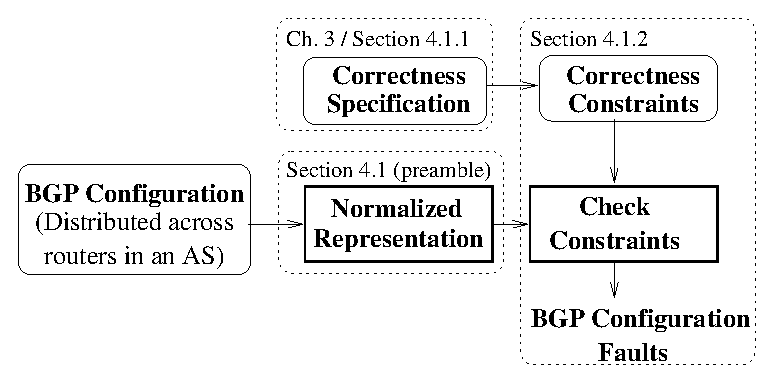
\epsfig{file=rcc/figures/rcc_arch.eps, width=0.9\linewidth}
\caption{Overview of \rccns.}
\label{fig:rcc_arch}
\end{figure}


%\subsection{Generating the Normalized Representation}

%\rcc normalizes BGP configuration to facilitate checking constraints.
\rcc implements the normalized representation as a set of relational
database tables.  This approach allows 
constraints to be expressed independently of router configuration
languages.  As configuration languages evolve and new ones emerge, only
the parser must be modified.  It also
facilitates testing network-wide properties, since all of
the information related to the network's BGP configuration can be
summarized in a handful of tables.  A relational structure is natural
because many sessions share common attributes (\eg, all sessions to the
same neighboring AS often have the same policies), and many policies
have common clauses (\eg, all eBGP sessions may have a filter that is
defined in exactly the same way).  Table~\ref{tab:if} summarizes these
tables; Section~\ref{sec:parser} details how \rcc populates them.

%; a more na\"{i}ve approach would require
%scanning all information about router loopback addresses and session
%information for every iBGP session.

\begin{table}[t]
\centering
%{\footnotesize
\begin{tabular}{lp{5in}}
{\bf Table} & {\bf Description} \\ \hline
%%%%%%%%%%%%%%%%%%%%
%router\_global & 
{\tft global options} & router, various global options (\eg, router ID)\\

%%%%%%%%%%%%%%%%%%%%
%sessions & 
{\tft sessions} & router, neighbor IP address, eBGP/iBGP,
pointers to policy, options (\eg, route-reflector client)\\ 

%%%%%%%%%%%%%%%%%%%%
%networks & 
{\tft prefixes} & router, prefix originated by this router\\

%%%%%%%%%%%%%%%%%%%%
%prefix\_acls & 
{\tft import/export filters} & normalized representation of filter:
IP range, mask range, permit or deny\\ 

%%%%%%%%%%%%%%%%%%%%
%route\_maps & 
{\tft import/export policies} & normalized representation of
policies \\
%; each policy represented by one or more rows
%; each row is a
%clause in the policy \\ 


%%%%%%%%%%%%%%%%%%%%
%router\_loopbacks & 
{\tft loopback address(es)} & router, loopback IP address(es)\\

%%%%%%%%%%%%%%%%%%%%
%router\_interfaces & 
{\tft interfaces} & router, interface IP address(es)\\


%%%%%%%%%%%%%%%%%%%%
%routes & 
{\tft static routes} & static routes for prefixes\\ \hdashline[1pt/1pt]

\multicolumn{2}{c}{{\bf Derived or External Information}} \\

%%%%%%%%%%%%%%%%%%%%
%parse\_errors & 
{\tft undefined references} & policies and filters that a
BGP configuration referenced but did not define\\

%%%%%%%%%%%%%%%%%%%%
%bogon\_list & 
{\tft bogon prefixes} & prefixes that should always be filtered on eBGP
sessions~\protect\cite{www-cymru-bogon}\\ 


%%%%%%%%%%%%%%%%%%%%
%%%%%%%%%%%%%%%%%%%%
%as_regexps & \\
%comm_regexps & \\ 
%communities & & \\ 
%router_sessions & \\
%sessions_shutdown & \\
\end{tabular}
%}
\caption{Normalized configuration representation.}
\label{tab:if}
\end{table}



\subsection{Applying the Correctness Specification to BGP Configuration} 
\label{sec:correct}

\rccns's correctness specification uses the properties from
Chapter~\ref{chap:rlogic} as a starting point. \rcc checks two aspects
of the correctness specification outlined in Chapter~\ref{chap:rlogic}:
{\em path visibility} and \emph{route validity}.  \rcc finds path
visibility and route validity violations in {\em BGP configuration
only}. To make general statements about path visibility and route
validity, \rcc assumes that the internal routing protocol (\ie, interior
gateway protocol, or ``IGP'') used to establish routes between any two
routers within a AS is operating correctly.  BGP requires the IGP to
operate correctly because iBGP sessions may traverse multiple IGP hops
and because the ``next hop'' for iBGP-learned routes is typically
several IGP hops away.

\rcc detects faults that cause {\em persistent} failures.  Both
Chapter~\ref{chap:rlogic} and previous work (\eg,~\cite{Griffin2002})
have studied conditions on the relationships between iBGP and
IGP configuration that must be satisfied to guarantee that iBGP
converges; \rcc does not yet parse IGP configuration, so it does not
check for violations of these constraints.
%
The correctness specifications and constraints assume that,
given stable inputs, the routing protocol {\em eventually} converges to
some steady state behavior.

Currently, \rcc only detects faults in the BGP configuration of a {\em
single AS} (a network operator typically does not have access to the BGP
configuration from other ASes).  Fortunately, because an AS's BGP configuration
explicitly controls both dissemination and filtering, many configuration
faults, including partitions, route leaks, etc., can be detected by
analyzing the BGP configurations of set of the routers in a single AS.


%We define constraints that must be satisfied to guarantee that the
%above properties hold.  For example, when a router imports a route
%from a neighboring AS, validity requires that it should not permit
%routes to prefixes that (1)~originate within its own as or (2)~are
%private or unallocated.  Similarly, when a router advertises a route
%to another router via iBGP, validity requires that the next-hop
%attribute of that route be reachable, and that every route along the
%IGP path to that next hop agree on the same next-hop.  To derive a
%reasonable set of tests, we perform this exercise for both validity
%and visibility for every step of BGP's operation.



%\subsection{Assumptions and Limitations}\label{sec:assumptions}

\subsection{Deriving Correctness Constraints and Detecting
  Faults}\label{sec:mapping} 


\begin{table}[t]
\hspace*{-0.1in}
\begin{center}
{\footnotesize
\begin{tabular}{@{}p{2in}p{3in}@{}}
{\bf Problem} & {\bf Possible Active Fault}\\ \hline \hline
%
\multicolumn{2}{@{}c@{}}{{\it Path Visibility}} \\ \hline
{\bf Dissemination Problems} \\
Signaling partition: & Router may learn a suboptimal route \\
\hspace*{0.1in} - of route reflectors &     or none at all. \\ 
\hspace*{0.1in} - within a RR ``cluster'' \\
\hspace*{0.1in} - in a ``full mesh'' \\

Routers with duplicate: & {Routers may incorrectly drop routes.} \\ 
\hspace*{0.1in} - loopback address \\ 
\hspace*{0.1in} - cluster ID \\

iBGP configured on one end & {Routers won't exchange
routes.} \\  
iBGP not to loopback & {iBGP session fails
when one interface fails.} \\  
%synchronization enabled & \parbox{2in}{iBGP route won't be used if the
%route doesn't also appear in IGP.} \\

\hline \hline
\multicolumn{2}{@{}c@{}}{{\it Route Validity}} \\ \hline
{\bf Filtering Problems} \\
transit between peers & \parbox{4in}{Network carries
traffic ``for free''.} \\
inconsistent export to peer & \parbox{2in}{Violation of contract.} \\
inconsistent import & \parbox{4in}{Possible unintentional
``cold potato'' routing.} \\
%{\bf Undefined References} \\
\parbox{2.18in}{
eBGP session: \\
\hspace*{0.1in} - w/no filters \\ 
\hspace*{0.1in} - w/undef. filter \\
\hspace*{0.1in} - w/undef. policy \\
filter: \\
\hspace*{0.1in} - w/missing prefix \\
policy: \\
\hspace*{0.1in} - w/undef. AS path \\
\hspace*{0.1in} - w/undef. community \\
\hspace*{0.1in} - w/undef. filter \\
}
& \parbox{3in}{
\begin{itemize}
\itemsep=-1pt
\item leaked internal routes
\item re-advertising bogus routes
\item accepting bogus routes from neighbors
\item unintentional transit between peers
\end{itemize}
}
\\
%\hdashline[1pt/1pt]



\hdashline[1pt/1pt]
{\bf Dissemination Problems} \\
prepending with bogus AS & \parbox{4in}{AS path is no longer valid.} \\
originating unroutable dest. & \parbox{4in}{Creates a blackhole.} \\ 
incorrect next-hop & {Other routers may be unable to reach
the routes for a next-hop that is not in the IGP.} \\

\hline\hline
\multicolumn{2}{@{}c@{}}{{\it Determinism}} \\ \hline


{\bf Ranking Problems} \\
\parbox{4in}{nondeterministic MED \\
age-based tiebreaking} 
& \parbox{4in}{Route selection depends on message order.}


\end{tabular}
}
\end{center}

\caption{BGP configuration problems that \rcc detects and their
potentially active faults.} 
\label{tab:rcc_tests}
\end{table}

Deriving constraints on the configuration itself that guarantee that the
correctness specification 
is satisfied is challenging. We reason about how the aspects of
configuration from Section~\ref{sec:semantics} affect each correctness
property and derive appropriate constraints for each of these aspects.
Table~\ref{tab:rcc_tests} summarizes the correctness
constraints that 
\rcc checks, which follow from determining which aspects of
configuration affect each aspect of the
correctness specification (from Section~\ref{sec:correct}).
These constraints are an attempt to map the path visibility and route
validity specifications to constraints on BGP configuration that can be
checked against the actual configuration.  


%Path visibility constraints typically address
%potential problems with how iBGP routes propagate through the AS, or
%``iBGP signaling'' (Section~\ref{sec:visibility}).  \rccns's route
%validity constraints test 
%potential problems with policy configuration or how routes are
%advertised (Section~\ref{sec:validity}).  
%The ``miscellaneous''
%constraints can affect both
%path visibility and route validity.
Ideally, operators would run \rcc to detect configuration faults {\em
before} they are deployed.  Some of \rccns's constraints detect faults
that would most likely become active immediately upon deployment.  For
example, a router that is advertising
routes with an incorrect next-hop attribute will immediately prevent
other routers that  
use those routes from forwarding packets to those
destinations.  In this case, \rcc can help a network operator diagnose
configuration faults and prevent them from introducing failures on the
live network.  
%Many constraints in Table~\ref{tab:rcc_tests} detect {\em
%latent} faults, detection of latent faults is very important because the
%operator may not unaware of an erroneous configuration until some input
%actually triggers the fault (at which time the failure can be quite
%serious).  

Many of the constraints in Table~\ref{tab:rcc_tests} concern faults that
could remain undetected even after the configuration has been deployed
because they remain masked until some sequence of messages triggers
them. In these cases, \rcc can help operators find faults that could
result in a serious failure.  Section~\ref{sec:visibility} describes one
such path visibility fault involving dissemination in iBGP in further
detail. 
%For example, an operator will likely not notice that a BGP
%session to a neighboring AS applies an undefined filter until that
%neighbor ``leaks'' an invalid route.  
%
In other cases, checking constraints implies some knowledge of high-level
policy (recall that route validity, as defined in
Definition~\ref{defn:rv}, concerns a path that conforms to some 
high-level policy).  In the absence of a high-level policy specification
language, 
\rcc must make inferences about a network operator's intentions.
Section~\ref{sec:validity} describes several route validity faults where
\rcc must make such inferences.


%\rcc checks the constraints against the normalized representation of the
%BGP configuration.  Section~\ref{sec:visibility} describes how \rcc uses
%the BGP session-level topology to detect path visibility faults in iBGP.
%Section~\ref{sec:validity} explains how \rcc uses beliefs and closures
%to detect route validity faults.  Section~\ref{sec:verifier} describes
%how \rcc checks these constraints in practice.


%\subsection{\rccl Architecture}\label{sec:design}



%% Describe architecture of the tool.  How we parse IOS/JunOS into an
%% intermediate format.  Describe the intermediate format, how we organize
%% checks in terms of mysql queries, etc. Three phases: 1. preparsing,
%% 2. parsing, 3. checking


%This section describes the high-level architecture of \rccns.  We
%present the design of \rccns's {\em intermediate configuration format},
%a vendor-independent representation of a network's BGP configuration.
%We then briefly describe the correctness tests that \rcc performs,
%noting how the intermediate configuration format facilitates many of
%these tests.



%\subsection{Verifying the Configuration}


%The intermediate format concisely represents configuration semantics and
%allows an operator to see the entire configuration at a glance.  The
%format implicitly specifies a model of network-wide routing
%configuration.  

%% We decided that the intermediate format should not make
%% any assumptions about how the network structure; rather, the
%% intermediate format should be a general, literal interpretation of the
%% configuration, and the queries against the intermediate format should
%% determine the semantics of the intermediate format.
%% %Accordingly, we had to decide
%% %whether the intermediate format should incorporate strict assumptions
%% %about the network configuration, or whether the format should be general
%% %enough to accept configurations that might not necessarily conform to
%% %the data model:
%% %
%% %\begin{itemize}
%% %\itemsep=-1pt
%% %\item What assumptions about network structure should be built into the
%% %intermediate format?  Should the format impose constraints on the
%% %configuration? 
%% %\end{itemize}
%% On one hand, incorporating strict assumptions about network structure
%% makes certain types of verification tests easier because the
%% intermediate format is guaranteed to conform to the strict model.
%% However, it also means that unorthodox configurations may not conform to
%% the model.  Adopting a more general structure allows unusual
%% configurations to be represented in the intermediate format, but it can
%% verification more difficult because the semantics of the intermediate
%% format are less explicit.

%% For example, the table of BGP sessions contains a column for a
%% ``remote AS''.  A remote AS is typically a unique number and represents a
%% distinct administrative domain, but, in certain cases,
%% the same remote AS may actually connect to {\em different} neighboring
%% networks: an ISP may assign the same AS number to multiple customers if
%% those customers have no other upstream providers.  
%% %In this case, the ISP
%% %should remove the ``customer'' AS number from the AS path before
%% %re-advertising the route.  
%% A single administrative domain
%% may also comprise multiple ASes~\cite{rfc-confederations}.

%% A strict data model might impose a one-to-one mapping between an AS and
%% an administrative domain, which would make certain
%% correctness tests easier: \rcc would know that all private AS numbers
%% should be removed on sessions to remote ASes, and, when comparing
%% policies across multiple sessions to the same AS number, it could know
%% that those policies were being applied to the same neighboring network.  
%% A more general data model would accept the configuration information,
%% even if the configuration was not sensible, and rely on the
%% verification process to report possible problems.  This approach
%% may cause the verifier to generate false positives: for example, the
%% verifier may wrongly report that a private AS should be removed from the
%% AS path of an ``eBGP'' session, when, in fact, the ``eBGP'' session is
%% a session to a router with a different AS number in the same
%% administrative domain.

%% Because BGP configuration is flexible, it is difficult to design a
%% strict format that will accept all sensible
%% configurations.  (In Section~\ref{sec:evaluation}, we will describe many
%% anomalies that \rcc discovered that illustrate that BGP can be
%% configured in many different ways to achieve the same task.)  We decided
%% that the
%% intermediate format should serve as a literal representation of the
%% configuration, without applying any sanity checks.  This decision has
%% worked well in practice: the fact that \rcc can load any configuration
%% into the intermediate format (rather than rejecting a configuration
%% because it does not fit the data model) allows it to be considerably
%% more usable.  Although this approach generates more false positives,
%% distinguishing more serious errors from ``anomalies'' has proved to be
%% relatively easy in practice.


%\subsection{Checking the Constraints}
%\label{s:verification}


\subsection{Completeness and Soundness}


\begin{figure}[t]
\centering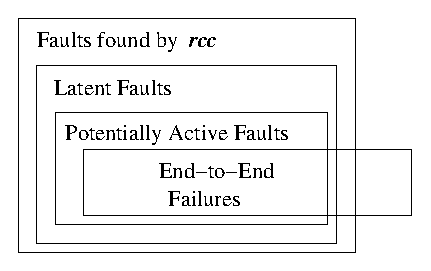
\epsfig{file=rcc/figures/faults2.eps, width=0.6\linewidth}
\caption{Relationships between faults and failures.}
\label{fig:faults}
\end{figure}

%% caveats and setting the fence
%\rccns's constraints are neither complete (\ie,
%they may not find all problematic configurations) nor sound (\ie, they
%may report problems that are simply deviations from best common
%practice), but static analysis techniques for program analysis
%are typically neither complete nor sound either~\cite{Musuvathi2003}.
%As discussed in Section~\ref{sec:mapping}, \rcc is neither complete nor
%sound.  
\rccns's constraints are neither complete nor sound; that is, they may
not find all problematic configurations, and they may complain about
harmless deviations from best common practice.  However, practical
static analysis techniques for program analysis are typically neither
complete nor sound, either~\cite{Musuvathi2003}.
Figure~\ref{fig:faults} shows the relationships between classes
of configuration faults and the class of faults that \rcc detects.  {\em
Latent faults} are faults that are not actively causing any problems but
nonetheless violate the correctness constraints.  A subset of latent
faults are {\em potentially active} faults, for which there is at least
one input sequence that is certain to trigger the fault.  For example,
an import policy that references an undefined filter on a BGP session to
a neighboring AS is a potentially active fault, which will be triggered
when that neighboring AS advertises a route that ought to have been
filtered.  When deployed, a potentially active fault will become {\em
active} if the corresponding input sequence occurs.  An active fault
constitutes a routing failure for that AS.

Some active faults may ultimately appear as {\em end-to-end failures}.
For example, if an AS advertises an invalid route (\eg, a route for a
prefix that it does not own) to a neighboring AS whose import policy
references an undefined filter, then some end hosts may not be able to
reach destinations within that prefix.  Note that a 
potentially active fault may not always result in an end-to-end failure
if no path between the sources and destinations traverses the routers in
the faulty AS.  

\rcc detects a subset of latent (and hence,
potentially active) faults.  In addition, \rcc
may also report some false positives: faults that violate the
constraints but are {\em benign} (\ie, the violations 
would never cause a failure).
Ideally, \rcc would detect fewer benign faults 
by testing the BGP configuration against an abstract specification.
Unfortunately,
producing such a specification requires additional work from
operators, and operators may well write incorrect specifications.  
One of \rccns's advantages is that it provides useful information about
configuration faults without requiring any additional work on the part
of operators.


Our previous work~\cite{Feamster2003b} presented three properties in
addition to path visibility and route validity: information flow control
(this property checks if routes ``leak'' in violation of policy),
determinism (whether a router's preference for routes depends on the
presence or absence of other routes), and safety (whether the protocol
converges)~\cite{Griffin2002c}.  Our definitions of route validity
(Definition~\ref{defn:rv}),
policy (Definition~\ref{defn:policy}), and policy-conformant paths
(Definition~\ref{defn:pcp}) incorporate the notion of information flow
control.  With a couple of exceptions (see Table~\ref{tab:rcc_tests}),
\rcc does not check for faults related
to determinism and safety.  Many aspects of determinism depend on the
route selection process that are inherent in today's practices (\eg, the
fact that MED is only comparable across routes received from the same
neighboring AS) and cannot be effectively checked using static analysis.
Safety is a property of the global routing system that, in practice,
requires access to configurations from multiple ASes to check.  In
Chapter~\ref{chap:policy}, we derive constraints that guarantee safety
with access to configurations of only a single AS and find that these
conditions are quite restrictive.


%\subsubsection{Intermediate Format Overview}








%%%%%%%%%%%%%%%%%%%%%%%%%%%%%%%%%%%%%%%%%%%%%%%%%%%%%%%%%%%%%%%%%%%%%%
%Since the intermediate format is simply a set of relational
%database tables, \rcc can check each correctness constraint by
%executing one ore more SQL queries against the database containing the
%configuration state.


%\footnote{We implemented all
%  correctness checks from 
%Section~\ref{sec:analysis} except those from previous
%work~\cite{Griffin2002}, which require knowledge about shortest
%IGP paths through the network, but, due to space constraints, we
%describe only two checks here: one ``single router'' check, and one that
%requires testing properties of the graph.}  

%Certain 
%queries involve comparing the entries from two tables. For example,
%\rcc checks whether every route that is originated by BGP has a
%corresponding route; this requires comparing entries in the {\tf
%networks} table against those from the {\tf routes} table.


%However, \rccns's extensible design
%facilitates adding these checks.

%% (might allude here to simple checks vs. complex checks)  not really
%% going to discuss pattern-based vs. whatever anymore.  simple checks
%% reall just entail checking bit-flips.  complex can involve multiple
%% routers, interaction with IGP, etc.

%% Also discuss the need to know default settings sometimes.  That is, even
%% the simple ``bit flip'' checks have subtleties.  For example, the avici
%% (and procket) story, where ``no sync'' is enabled by default.  An ideal
%% version of the checker should keep track of routing vendor, OS version
%% numbers, etc., and a detailed list of what's enabled/disabled by default
%% for a particular router.



%%\subsection{\rccl Intermediate Configuration Format}\label{sec:if}









%Note that we do {\em not}
%assume that BGP converges: its steady state for a fixed input
%might be oscillatory.


%\subsubsection{Challenges}\label{sec:challenges}

%BGP configuration errors are difficult to detect because they often
%appear far from the actual source of the error and may not appear
%immediately after the deployment of an erroneous configuration.
%(Sections~\ref{sec:validity} and~\ref{sec:visibility} discuss at greater
%length configuration errors that are not immediately apparent.)  As a
%result, operators must often search for errors in a trial-and-error
%fashion.

%\rcc performs both ``basic'' single-router configuration checks and more
%complicated network-wide checks.  We discovered that even syntactic
%errors on a single router often fail silently: in one network, \rcc
%found a session that applied an undefined filter that would have allowed
%that AS's customer to advertise any prefix.  These types of errors are
%relatively easy to find because they only involve looking at single
%configuration files in isolation.
%%\footnote{Previous work
%% single-router checks that do not specifically address
%%the correctness of any particular protocol~\cite{FeldmannXXXX}; we
%%perform similar checks for BGP and extend
%%this work in several ways: 
%%(1)~we report statistics on the errors we have found in practice; (2)~we
%%have made our tool publicly available to network operators; and (3)~our
%%tool is in use by many ISPs.}.  
%Analyzing the {\em network-wide} behavior of BGP configuration, on the
%other hand, requires synthesizing configuration across all of the
%routers in the AS, which presents several challenges:
%\begin{CompactEnumerate}

%\item {\em BGP configuration is distributed.}  Verifying BGP
%  configuration requires checking dependencies across multiple routers.
%  For example, determining how (and whether) routes propagate between
%  routers requires parsing the configurations of every router in the
%  network to construct an {\em session-level graph} of iBGP sessions, as well
%  as determining how policies are applied on each of those sessions (and
%  how the policies relate to one another).

%\item {\em BGP configuration is network-specific.}  BGP
%  configuration is flexible enough to allow network operators to
%  implement the same behavior in many different ways.  In fact, an
%  operator may implement the {\em same} policy in several different ways
%  on routers in the same AS.  \rcc must {\em canonicalize} BGP
%  configuration by representing it in some normalized format.

%\item {\em BGP configuration is vendor-specific.}  Any single AS may may
%  use routers from several different router vendors: nearly every
%  network we analyzed used at least two router vendors, and one small
%  ISP we analyzed used routers from four different vendors.  To analyze
%  these networks, \rcc must be able to represent BGP configuration in
%  some {\em vendor-independent} format.  In practice, designing such a
%  format is tricky: Vendor configuration languages have vastly different
%  syntax and even have slight differences in semantics.  For example, in
%  Cisco IOS, the next-hop attribute is assigned as a session-level
%  option, whereas in JunOS, the next-hop is assigned in policy statements.

%\end{CompactEnumerate}

%To address these challenges, we represent the network-wide set of
%configuration files as a collection of database tables.  This
%normalized format allows \rcc to quickly access information about
%groups of BGP sessions or policies and makes the verification process
%independent from configuration syntax and specifics.  We describe the
%normalized format in more detail in Section~\ref{sec:parsing}.


%% We address these challenges by viewing BGP as a distributed program,
%% rather than a protocol that conforms to a set specification.\footnote{We
%% explain in Section~\ref{s:related} why the absence of a 
%% specification makes verifying wide-area routing using
%% approaches like model checking infeasible.}  We determine a set of
%% invariants that 
%% should hold true independent of the details of configuration.  Many of
%% these invariants are verifiable using static analysis.
%% %
%% We also determine which invariants require checking configurations at a
%% single router and which require checks across multiple routers.
%% Fortunately, we find that many serious problems can be uncovered with
%% checks that only require configurations from routers {\em within a
%% single network}.
%\footnote{Griffin and Wilfong's ``safety'' violation
%caused by incompatible policies in different networks is an
%exception~\cite{Griffin2002c}; see Section~\ref{s:safety}.}  

%% \item {\em Defining ``correctness'' is difficult.}  Operators configure BGP
%% to achieve a variety of tasks.  Defining
%% ``correctness'' for a protocol that can behave in many ways is
%% difficult.  We use the {\em routing logic}~\cite{Feamster2003b} to help
%% us define correctness properties and constraints.



%\rcc performs static analysis on a set of BGP configurations from
%routers in a single AS and outputs a list of faults.
%Figure~\ref{fig:rcc_arch} illustrates this approach.  
%Section~\ref{sec:correct} defines a specification for two aspects of
%routing correctness---path visibility and
%route validity.
%\rcc normalizes
%vendor-specific router configurations into an normalized
%format (Section~\ref{sec:parsing}),
%analyzes the normalized format
%(Section~\ref{s:verification}), and produces a list of faults.



%In
%fact, we believe that it is highly unlikely that network operators would
%have paid attention to \rcc had it not been software that works ``out of
%the box'' on existing configurations without requiring any other
%operator input.


%\rcc detects faults by testing a set of
%constraints on BGP configuration based on the correctness specification
%we propose in Section~\ref{sec:correct} and outlined in more detail in
%Section~\ref{s:verification}.  These faults may be latent 
%(some of these are potentially active), but \rcc may also find {\em
%benign} (\ie, false positives).  \rcc is also not guaranteed to catch
%all latent faults.  



%%% Set the fence here

%
%A {\em potentially active fault} is a latent fault for 
%A latent fault is a {\em potentially active fault} if it may
%cause BGP to violate correctness, but may require a particular execution
%path to
%actually cause a violation.  
%



%% Why is this task challenging?
%% Analyzing BGP routing is akin to analyzing a distributed program,
%% because most (if not all) faults that occur in practice are caused by
%% statements in router configurations.  Because BGP configuration is
%% distributed, analyzing the network-wide behavior of a set of routers
%% requires the ``joint analysis'' of their configurations and an
%% assessment of the interactions and dependencies between them.
%% Additionally, configuration languages are flexible: the same high-level
%% routing behavior (\eg, a particular policy) can be implemented in
%% multiple ways on a given set of routers.  In addition, each router
%% vendor has a different configuration language, and these languages are
%% not entirely feature-compatible.  \rcc addresses these challenges by
%% using a vendor-independent normalized configuration format based on
%% the relational data model.

%% move to related work
%Other tools perform some
%single-router consistency checks that catch fundamental
%mistakes~\cite{Caldwell2003}, 
%%but verifying BGP correctness requires
%%analyzing a {\em network-wide} view of configuration and a {\em
%%definition of correctness}.  \rcc executes network-wide correctness
%%checks based on a high-level definition of correctness.


%We believe that one reason that
%\rcc has enjoyed a relatively high level of acceptance is because it
%works ``out of the box'': it provides useful information to network
%operators while requiring no additional effort on their part.


%\subsection{Approach}

%Figure~\ref{fig:rcc_arch} illustrates the \rccns's high-level approach
%to BGP configuration checking.  \rcc expects a set of router
%configurations from a single AS, which can be collected from the routers
%using existing tools such as ``rancid''~\cite{www-rancid}.  Ultimately,
%\rcc outputs information that helps operators track down BGP
%configuration errors.  To do this, \rcc must first have a set of
%properties to check;  describes our high-level
%approach for describing these checks.  Because \rcc attempts to make
%statements about a single protocol using only the configurations, it
%must make some assumptions, which we describe in
%Section~\ref{sec:assumptions}.  Section~\ref{sec:challenges} explains
%why checking properties of distributed router is
%difficult in practice.

\section{Path Visibility Faults}\label{sec:visibility}

Recall that {\em path visibility} specifies that every router that has a
usable path to a destination learns at least one valid route to that
destination (Definition~\ref{defn:pv}). It is an important property
because it ensures that, if the network remains connected at lower
layers, the routing protocol does not create any network partitions.
Table~\ref{tab:rcc_tests} shows many conditions that \rcc checks related
to path visibility; in this section, we focus on iBGP configuration
faults that can violate path visibility and explain how \rcc detects
these faults.

%Routers within an AS disseminate eBGP-learned routes to
%other routers in the AS using iBGP.  
%If two routers in the same AS have the same loopback address, visibility
%can be violated if one of those routers hears a route from the
%other, and discards it, thinking it advertised the route itself.
%The simplest approach is to propagate routes within the AS involves
%configuring iBGP 
%sessions between every pair of BGP-speaking routers within the AS, (a
%``full-mesh'' topology), where each router selects a best route from
%among its available choices and, if that route was learned via eBGP,
%readvertises that route over its iBGP sessions.  

Ensuring path visibility in a ``full mesh'' iBGP topology (as described
in Section~\ref{sec:dissemination}) is reasonably
straightforward; \rcc checks that every router in the AS has an iBGP
session with every other eBGP-speaking router.  If this condition is
satisfied, every router in the AS will learn all eBGP-learned routes.

%Because a ``full mesh'' iBGP topology scales poorly, operators often
%employ {\em route reflection}~\cite{rfc2796}.  A subset of the
%routers are configured as {\em route reflectors}, with the configuration
%specifying a set of other routers as {\em route reflector clients}.
%Each route reflector readvertises its best route according to the
%following rules: (1)~if the best route was learned from an iBGP peer,
%the route is readvertised to all of its route reflector clients; (2)~if
%it was 
%learned from a client or via an eBGP session, the route is readvertised
%on all iBGP sessions.  
%If a route reflector client has
%multiple route reflectors, those reflectors must share all of their
%clients and belong to a single ``cluster''.

A route reflector may itself be a client of another route reflector.
Any router may also have iBGP sessions with other routers.
Recall from Section~\ref{sec:visibility_def} that we use the set of
reflector-client relationships between routers in an AS to define a 
graph $\I$, where each router is a node and each
session is either a directed or undirected edge: a client-reflector
session is a directed edge from 
reflector to client, and other iBGP sessions are undirected edges.  An
edge exists if and only if (1)~the configuration of each router endpoint
specifies the loopback address of the other endpoint\footnote{If a
router establishes an iBGP session with a router's {\em loopback} address,
then the iBGP session will remain active as long as that router is
reachable via {\em any} IGP path between the two routers.  If a router
establishes an iBGP session with an interface address of another router,
however, the iBGP session will go down if that interface fails, even if
an IGP path exists between those routers.} and (2)~both routers agree
on session options (\eg, MD5 authentication parameters).  $\I$
should also not have partitions at lower layers.  We say that $\I$ is
{\em acyclic} if $\I$ has no sequence of directed and undirected edges
that form a cycle.  

\begin{figure}[t]
\begin{center}
\begin{psfrags}
\psfrag{r1}{{\Large Route $r_1$ to $d$}}
\psfrag{r2}{{\Large Route $r_2$ to $d$}}
\psfrag{RR1}{{\LARGE $RR_1$}}
\psfrag{RR2}{{\LARGE $RR_2$}}
\psfrag{W}{{\LARGE $W$}}
\psfrag{X}{{\LARGE $X$}}
\psfrag{Y}{{\LARGE $Y$}}
%\centering
\begin{pspicture}(8,3.5)
%    \showgrid
    \psset{nodesep=2pt, arrows=->}

    \cnodeput(2.875,3.05){W}{$W$}
    \cnodeput(6,2.1){Y}{$Y$}
    \cnodeput(2,2.1){c1}{\hspace{0.12in}}
    \cnodeput(3.75,2.1){c2}{$X$}%\hspace{0.12in}}
    \cnodeput(6.875,1.15){c3}{$Z$}

    \ncline{c1}{W}
    \ncline{c2}{W}
    \ncline{c3}{Y}

    \psset{nodesep=2pt, arrows=-}
    \ncline{c2}{Y}


    \rput(2.875,4){\rnode{r1}{{\small route $r_1$ to $d$}}}
    \rput(3.75,0.25){\rnode{r2}{{\small route $r_2$ to $d$}}}

    \psset{nodesep=1pt, linestyle=dashed, arrows=<-}
    \ncline{W}{r1}
    \ncline{c2}{r2}%\rput(1.25,0.5){\rnode{w2}{$w_2$}}

    \rput(4.55,3.25){\rnode{rrc}{{\small Route Reflector (RR)}}}
    \rput(4.15,2.55){\rnode{rrc}{{\small Client}}}

    \rput(6.5,2.35){\rnode{rrc}{{\small RR}}}
    \rput(7.23,1.6){\rnode{rrc}{{\small Client}}}


    \psframe[fillcolor=white,linestyle=dashed, framearc=0.3](1.25,0.75)(7.75, 3.5)


\end{pspicture}

\resizebox{0.55\linewidth}{!}{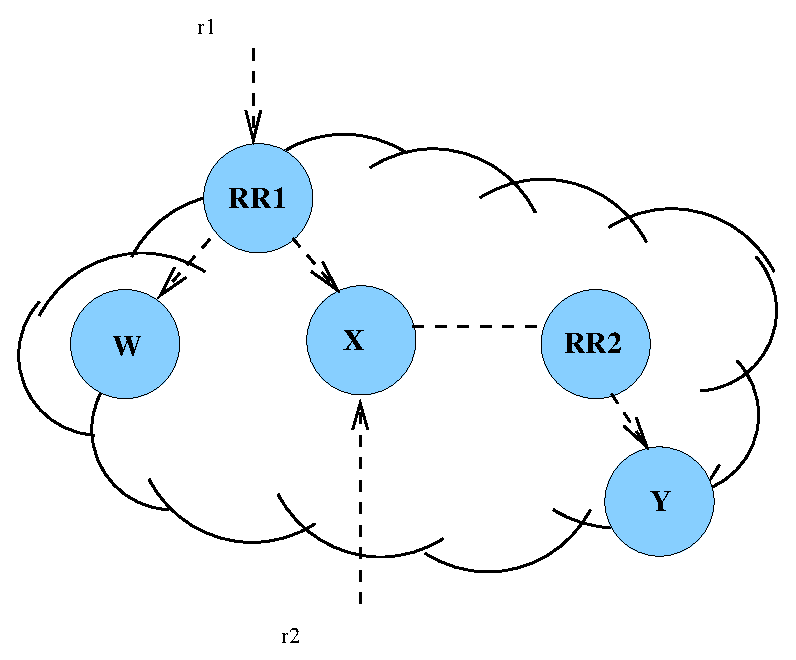
\includegraphics{rcc/figures/rr_example_fig2.eps}}
\end{psfrags}
\end{center}
\caption[An iBGP route reflector topology that violates path visibility.]{
In this iBGP configuration, route
$r_2$ will be distributed to all the routers in the AS, but
$r_1$ will not.  $RR_2$ and $Y$ will not learn of $r_1$, leading to a
network partition that won't be resolved unless another route to
the destination appears from elsewhere in the AS.}
\label{f:ibgp_vis_violation}
\end{figure}

%% \begin{figure}
%% \centering
\begin{pspicture}(8,3.5)
%    \showgrid
    \psset{nodesep=2pt, arrows=<->}

    \cnodeput(2,2.75){WC1}{$WC_1$}
    \cnodeput(1,1.6){WC2}{$WC_2$}
    \cnodeput(3,1.35){WC3}{$WC_3$}
    \cnodeput(6.25,2.75){EC1}{$EC_1$}


    \ncline{WC1}{WC2}
    \ncline{WC2}{WC3}
    \ncline{WC3}{WC1}

    \ncline{WC1}{EC1}
    \ncline{WC2}{EC1}
    \ncline{WC3}{EC1}

    \rput(1,0){\rnode{pw2}{}}
    \rput(3,0){\rnode{pw3}{}}
    \rput(6.25,0){\rnode{pe1}{}}


    \psset{nodesep=2pt, linestyle=dotted, arrows=<->}
    \ncline{WC2}{pw2}\rput(1.25,0.5){\rnode{w2}{$w_2$}}
    \ncline{WC3}{pw3}\rput(3.25,0.5){\rnode{w3}{$w_3$}}
    \ncline{EC1}{pe1}\rput(6.5,0.5){\rnode{e1}{$e_1$}}



    \psset{nodesep=0pt, arrows=-}

    \psframe[fillcolor=white,linestyle=dashed, framearc=0.3](0.25,0.75)(7.5, 3.5)


\end{pspicture}

%% \caption{BGP connectivity diagram for an AS with three routers on the
%%   west coast and one on the east coast.  Solid lines denote iBGP
%%   sessions, and dotted lines denote eBGP sessions.}
%% \label{fig:visibility_example}
%% \end{figure}

Even a connected directed acyclic graph of iBGP sessions can violate
path visibility.  For example, in Figure~\ref{f:ibgp_vis_violation},
routers $RR_2$ and $Y$ do not learn route $r_1$ to destination $d$ (learned
via eBGP by router $RR_1$), because $X$ will not readvertise routes learned
from its iBGP session with $RR_1$ to other iBGP sessions.  We call this
path visibility fault an {\em iBGP signaling partition}: a
path exists, but neither $RR_2$ nor $Y$ has a route for it.  Note that
simply adding a regular iBGP session between routers $RR_1$ and $RR_2$ would
solve the problem.

%This potentially active fault can
%prevent routers from learning any route to a destination, even
%though a path exists.  
In addition to causing network partitions, iBGP signaling partitions may
result in suboptimal routing.
For example, in Figure~\ref{f:ibgp_vis_violation}, even if $RR_2$ or $Y$
learned a route to $d$ via eBGP, that route might be worse than
the route learned at $RR_1$.  In this case, $RR_2$ and $Y$ would ultimately
select a suboptimal route to the destination, an event that an operator
would likely fail to notice.


%
%% Visibility violations have the potential for hard-to-detect network
%% partitions (mainly because the location of the problem could be far
%% from the place the misconfiguration has happened).  There are other
%% problems caused by lack of visibility too, as shown in
%% Figure~\ref{fig:visibility_example}.  Assume that $w_2$, $w_3$, and
%% $e_1$ are eBGP sessions to the same neighboring AS that advertises a
%% route to destination $d$.  If router $EC_1$ were misconfigured such
%% that it was not readvertising its routes to the $WC$ routers, then
%% none of the $WC$ routers would be able to reach $d$, even though a
%% valid path to $d$ exists via $EC_1$.  Moreover, if the AS in the
%% figure has routers separated by long-haul links (\eg the ``WC''
%% routers were on the West Coast of the US and the ``EC'' routers were
%% on the East Coast), and the route to $d$ were not advertised by either
%% $WC_2$ or $WC_3$, then these routers would send packets to $d$ via
%% $EC$ instead of sending packets via the nearest available exit point.
%% In this example, if the $WC_1\leftrightarrow WC_2$ and
%% $WC_1\leftrightarrow WC_3$ sessions were non-existent or had failed,
%% then $WC_1$ would choose the sub-optimal route to $d$ via $e_1$.
%

\rcc detects iBGP signaling partitions.
It determines if there is {\em any}
combination of eBGP-learned routes such that at least one router in the
AS will not learn at least one route to the destination, by performing a
check based on the following result, which we proved in
Section~\ref{sec:visibility_def}. 

\vskip 0.1in
%\begin{theorem}\label{thm:vis}

\noindent {\bf Theorem~\ref{thm:vis}.} 
{\em Suppose that the graph defined by an AS's iBGP relationships, $\I$, is
acyclic.  Then, $\I$ does not have a signaling partition if, and only
if, the eBGP-speaking routers that are not route reflector clients form
a clique. }
%\end{theorem}
\vskip 0.1in

%% \begin{proof}
%% Call the set of routers that are not reflector clients the
%% ``top layer'' of $G$.  If the top layer is not a full mesh,
%% then there are two routers $X$ and $Y$ with no iBGP session between
%% them, such that no route learned using eBGP at $X$ will ever be
%% disseminated to $Y$, since no router readvertises an
%% iBGP-learned route.

%% Conversely, if the top layer is a full mesh, observe that {\em if} a
%% route reflector 
%% has a route to the destination, then all its clients
%% have a route as well.  Thus, if every router in the
%% top layer has a route, all routers in the AS will have a route.  If any
%% router in the top layer learns a route through eBGP, then all the
%% top layer routers will hear of the route (because the top layer is a
%% full mesh).  Alternatively, if no router at the top layer hears an
%% eBGP-learned route, but some other router in the AS does, then that
%% route propagates up a chain of route reflectors (each client sends it to
%% its reflector, and the reflector sends it on all its iBGP sessions) to
%% the top layer, from there to all the other top layer routers, and from
%% there to the other routers in the AS.
%% \end{proof}


\rcc checks this condition by constructing the iBGP signaling
graph $\I$ from the {\tf sessions} table (Table~\ref{tab:if}). It assumes
that the IGP graph is connected, then determines whether $\I$ is
connected and acyclic and whether the routers at the top layer of $\I$ form
a clique.


\section{Route Validity Faults}\label{sec:validity}

BGP should satisfy {\em route validity}, as defined formally in
Chapter~\ref{chap:rlogic} (Definition~\ref{defn:rv}).
%BGP configuration affects which routes each router accepts, selects, and
%readvertises.  
Table~\ref{tab:rcc_tests} summarizes the route validity faults that \rcc
checks.  The biggest challenge for checking route validity is
that the definition says that the routes the routers in an AS select
should induce only policy-conformant paths (see
Definition~\ref{defn:pcp}), but \rcc operates without a specification of
the intended policy.  This section focuses on \rccns's approach to
detecting potential policy-related problems.

Requiring operators to provide a high-level policy specification would
require designing a specification language and convincing operators to
use it, and it provides no guarantees that the results would be more
accurate, since errors may be introduced into the specification itself.
Instead, \rcc forms {\em beliefs} about a network operator's intended
policy in two ways: (1)~assuming that intended policies conform to best
common practice and (2)~analyzing the configuration for common patterns
and looking for deviations from those patterns.  (The idea of forming
beliefs about intended protocol behavior is inspired from similar ideas
in systems~\cite{Engler01}.)  \rcc then finds cases
where the configuration appears to violate these beliefs.  It is
noteworthy that, even in the absence of a policy specification, this
technique detects many meaningful configuration faults and generates few
false positives.

%% An AS's customers will sometimes advertise smaller prefixes to its upstream
%% AS to load balance its inbound traffic, but it will tag those prefixes
%% with an instruction to its upstream to not readvertise these
%% prefixes~\cite{rfc1997}.  The export policies on an AS's routers should
%% always ensure that such a route is not readvertised to any neighbors.
%% Network operators also control the export of routes between
%% their peers and providers.  Static analysis can check this property by
%% analyzing the configuration files to verify that every eBGP session has
%% a filter that matches routes that have this instruction and prevents
%% them from being readvertised to other ASes.

\subsection{Violations of Best Common Practice}

We can derive some notions of high-level policy from our knowledge of
best common practice (\ie, the manner in which many ASes
tend to configure their 
networks).  In particular, \rcc looks for two violations of best common
practice: (1)~advertising a route from one ``peer'' to another (\ie, a
violation of the common business practices defined in
Table~\ref{tab:business} (Section~\ref{sec:semantics}); and (2)~not
advertising routes in a consistent manner at all peering
points~\cite{Feamster2004b}.  In this section, we explain both of these
practices in more detail.

A route that an AS learns from one of its ``peers'' should not be
readvertised to another peer.  Checking this condition requires
determining how a route propagates through an AS.
Figure~\ref{fig:policy_closure} illustrates how \rcc performs this
check.  Suppose that \rcc is analyzing the configuration from AS $X$ and
needs to determine that no routes learned from AS $B$ are exported to
AS $A$.  First, \rcc determines all routes that AS $X$ exports to AS $A$,
typically a set of routes that satisfy certain constraints on their
attributes. For example, router $R_1$ may export to AS $A$ only routes
that are ``tagged'' with the label ``$1000$''.  As described in
Section~\ref{sec:conf}, ASes often assign such ``community'' labels to a
route to
control how other routers rank or filter it. \rcc then checks the {\em
import} policies for all sessions to AS $B$, ensuring that no import
policy will set route attributes on any incoming route that would place
it in the set of routes that would be exported to AS $A$.  To perform
this check, \rcc must know which of an AS's neighboring ASes are peers;
thus, this check requires this additional input from the network
operator.

Additionally, an AS should advertise routes with equally good attributes
to each peer at every peering point.  An AS should not advertise routes
with inconsistent attributes, since doing so may prevent its peer from
implementing ``hot potato'' routing:
If ASes $1$ and $2$ are
peers, then the export policies of the routers in AS $1$ should export
routes to AS $2$ that have equal AS path length and MED values.  If not,
router $X$ could be forced to send traffic to AS $1$ via router $Y$
(``cold potato'' routing).
This behavior typically violates peering
agreements.  Recent work has observed that this type of inconsistent
route advertisement sometimes occurs in practice~\cite{Feamster2004b}.

An AS's policies may violate this best common practice for two reasons.
First, an AS may apply different export policies at different routers to
the same peer.  Checking for consistent export involves comparing export
policies on each router that has an eBGP session with a particular peer.
Static configuration analysis is useful because it can efficiently
compare policies on 
many different routers.  In practice, this comparison is not
straightforward because differences in policy definitions are difficult
to detect by direct inspection of the distributed router configurations.
\rcc facilitates comparing export policies across sets of routers by
normalizing all of the export policies for an AS, as described in
Table~\ref{tab:if} (Section~\ref{sec:rcc_overview}).  Second, an iBGP
signaling partition can 
create inconsistent export policies because routes with equally good
attributes may not propagate to all peering routes.  For example,
consider Figure~\ref{f:ibgp_vis_violation} again.  If routers $W$ and
$Z$ both learn routes to some destination $d$, then route $W$ may learn
a ``better'' route to $d$, but routers $Y$ and $Z$ will continue to
select the less attractive route.  If routers $X$ and $Y$ readvertise
their routes to a peer, then the routes advertised by $X$ and $Y$ will
not be equally good.  Thus, \rcc also checks whether routers that
advertise routes to the same peer are in the same iBGP signaling
partition (as described in Section~\ref{sec:visibility}, \rcc checks for
all iBGP signaling partitions, but ones that cause inconsistent
advertisement are particularly serious).

\subsection{Configuration Anomalies}

\begin{figure}
\begin{center}
\begin{psfrags}
\psfrag{AS A}{AS $A$}
\psfrag{AS B}{AS $B$}
\psfrag{AS X}{{\LARGE AS $X$}}
\psfrag{R1}{$R_1$}
\resizebox{0.85\textwidth}{!}{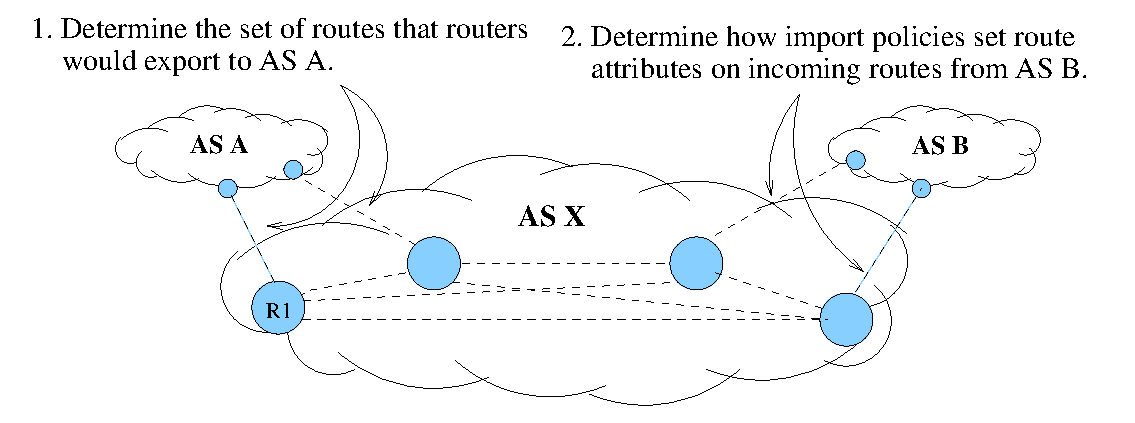
\includegraphics{rcc/figures/policy_closure.eps}}
\end{psfrags}
\end{center}
\caption{How \rcc computes route propagation.}
\label{fig:policy_closure}
\end{figure}

When the configurations for sessions at different routers to a
neighboring AS are the same except at one or two routers, the deviations
are likely to be mistakes.  This test relies on the belief that, if an
AS exchanges routes with a neighboring AS on many sessions and most of
those sessions have identical policies, then the sessions with slightly
different policies may be misconfigurations.  Of course, this test could
result in many false positives because there are legitimate reasons for
having slightly different import policies on sessions to the same
neighboring AS (\eg, outbound traffic engineering), but it does provide
a useful sanity check.

%% that all
%% routes received from a peer look equally good up to the IGP tiebreak
%% step, thus allowing it to use nearest exit (``hot potato'') routing with
%% its peers.  Of course, an AS cannot ensure that it receives AS paths of
%% equal length at all peering points with its peer, but it can take
%% precautions such as resetting the MED value on import and ensuring that
%% the local preference value is the same everywhere.  


\section{Implementation}\label{sec:implementation}


\begin{figure}[t]
\centering
%\begin{pspicture}(8,1.25)
%\showgrid
\rput(1,1.25){\rnode{config}{\parbox{1.3in}{\centering{\mft Router
	Configurations\\ (offline, collected from routers)}}}}
\rput(7,1.25){\rnode{prop}{{\mft Property}}}
\rput(0.25,0.25){\rnode{rs}{\psframebox{\parbox{0.5in}{\centering{\mft Preprocessor}}}}}
\rput(3.3,0.25){\rnode{sim}{\psframebox{\parbox{0.5in}{\centering{\mft Parser}}}}}
\rput(6.65,0.25){\rnode{la}{\psframebox{\parbox{0.5in}{\centering{\mft
	  Verifier}}}}}
\rput(8,0.25){\rnode{end}{}}
\ncline[arrows=->]{rs}{sim}
\ncline[arrows=->]{sim}{la}
\ncline[arrows=->]{la}{end}
\ncarc[arrows=->,nodesep=2pt]{prop}{la}
\ncarc[arrows=->]{config}{rs}
\rput(2.15,0.55){\parbox{0.85in}{{\dft Processed Input}}}
\rput(5,0.55){\parbox{0.55in}{\centering{\dft Intermediate Format}}}
\rput(7.95,0.55){{\dft Error?}}
\end{pspicture}

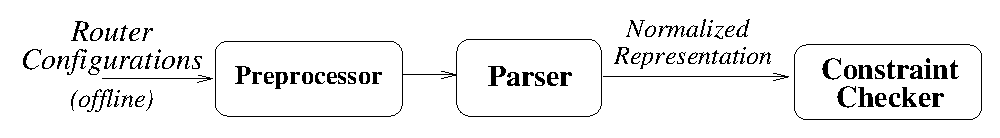
\epsfig{file=rcc/figures/rcc_design.eps, width=\linewidth}
\caption{Overview of \rcc implementation.}
\label{fig:rolex_design}
\end{figure}

\rcc is implemented in 
%about 6,500 lines of 
Perl and has been downloaded
by over seventy network operators.
The parser is roughly
60\% of the code.  
Much of the parser's logic is dedicated to policy
normalization.  
%
Figure~\ref{fig:rolex_design} shows an overview of \rccns, which 
takes as input the set of configuration files collected from
routers in a single AS
using a tool such as ``rancid''~\cite{www-rancid}.
\rcc
converts the vendor-specific BGP configuration to a vendor-independent
normalized 
representation.  It then checks this normalized format for faults
based on a set of correctness constraints.  
\rccns's functionality is
decomposed into three distinct modules: (1)~a preprocessor, which
converts configuration into a more parsable version; (2)~a parser, which
generates the normalized  representation; and (3)~a constraint checker,
which checks the constraints.  



\begin{figure}[t]
\centering
\hspace*{-0.2in}
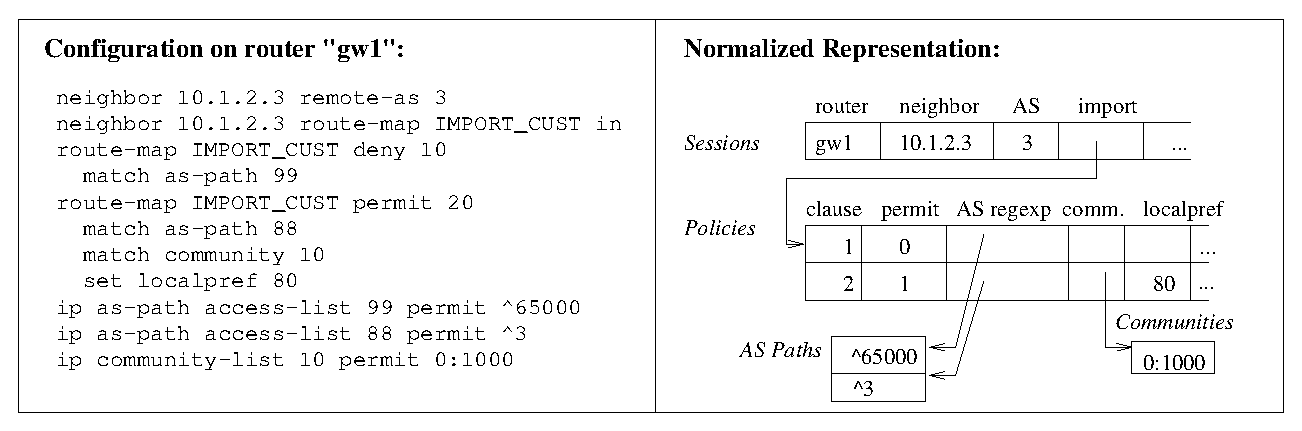
\epsfig{file=rcc/figures/if.eps, width=0.95\linewidth}
\caption{BGP configuration in normalized format.} 
\label{fig:if}
\end{figure}

\subsection{Preprocessing and Parsing}\label{sec:parser}

The {\em preprocessor} adds scoping identifiers to configuration
languages that do not have explicit scoping (\eg, Cisco IOS) and expands
macros (\eg, Cisco's ``peer group'', ``policy list'', and ``template''
options).  After the preprocessor performs some simple checks to
determine whether the configuration is a Cisco-like configuration
or a Juniper configuration, it launches the appropriate parser.  Many
configurations (\eg, Avici, Procket, Zebra, Quarry) resemble Cisco
configuration; the preprocessor translates these configurations so that
they more closely resemble Cisco syntax.

The {\em parser} generates the normalized representation from the
preprocessed configuration.  
%\rcc parses Cisco and
%Juniper configurations, as well as the configurations of other vendors
%that are loosely based on Cisco configuration syntax (\eg, Cisco,
%Procket, Quarry, etc.).  
The parser processes each router's configuration independently.  It
makes a single pass over each router's configuration, looking for keywords
that help determine where in the configuration it is operating (\eg,
``{\tt route-map}'' in a Cisco configuration indicates that the parser
is entering a policy declaration).  The parser builds a table of
normalized policies by
dereferencing all filters and other references in the policy; if the
reference is defined after it is referenced in the same file, the
parser performs lazy evaluation.  When it reaches the end of a file, the
parser flags any policies references in the configuration that it was
unable to resolve.  The parser proceeds file-by-file (taking care to
consider that definitions are scoped by each file), keeping track of
normalized policies and whether they have already appeared in other
configurations. 

Figure~\ref{fig:if} shows \rccns's normalized representation for a
fragment of Cisco IOS.  In \rccns, this normalized representation is
implemented as a set of mySQL database tables corresponding to the
schema shown in Table~\ref{tab:if}.  This Cisco configuration specifies
a BGP session to a neighboring router with IP address {\tt 10.1.2.3} in
AS 3.  This statement is represented by a row in the {\tf sessions}
table.  The second line of configuration specifies that the import
policy (\ie, ``route map'') for this session is defined as ``{\tt
IMPORT\_CUST}'' elsewhere in the file; the normalized representation
represents the import policy specification as a pointer into a separate
table that contains the import policies themselves.  A single policy,
such as {\tt IMPORT\_CUST}, is represented as multiple rows in the {\tf
policies} table.  Each row represents a single clause of the policy.  In
this example, {\tt IMPORT\_CUST} has two clauses: the first rejects all
routes whose AS path matches the regular expression number ``$99$''
(specified as ``{\tt \^{}65000}'' elsewhere in the configuration), and
the second clause accepts all routes that match AS path number ``$88$''
and community number ``$10$'' (\ie, {\tt 0:1000}) and sets the ``local
preference'' 
attribute on the route to a value of $80$.  Each of these clauses is
represented as a row in the {\tf policies} table; specifications for regular
expressions for AS paths and communities are also stored in separate
tables, as shown in Figure~\ref{fig:if}.

\rccns's normalized representation does not store
the names of the policies themselves (\eg, ``{\tt IMPORT\_CUST}'', AS
regular expression number ``88'', etc.).  Rather, the normalized format
only stores a description of what the route policy does (\eg, ``set the
local preference value to $80$ if the AS path matches regular expression
{\tt \^{}3}'').  Two policies may be written using entirely different
names, regular expression numbers, or even in different languages, but
if the policies perform the same operations, \rcc will recognize that
they are in fact the same policy.

%This process of {\em policy canonicalization} makes
%distinguishing policies across multiple routers trivial.  Without this
%normalization, ``eyeballing'' router configurations is not
%easy: policies that have the same name on two different routers may
%perform entirely different operations, and vice versa.  
%We have observed
%this practice surprisingly often.





%% Thus, even if two
%% policies are named differently on two different routers, the
%% canonicalization will reveal that the policies are identical.
%% The parser also recognizes when policies on routers with the
%% same names and reference names are different when the policies actually
%% perform different operations.

%% The {\tf global options}, {\tf sessions}, and {\tf prefixes} tables are
%% populated from statements within the BGP section of the configuration
%% files (\eg, {\tt router bgp} in Cisco configuration).  Other tables are
%% populated by parsing the appropriate sections of the configuration.
%% Populating the {\tf policies} and {\tf filters} tables is more
%% complicated.  \rcc compares policies {\em across} routers; thus, it
%% requires a concise, normalized, step-by-step policy specification.  This
%% process generates a normalized ``pseudocode'' representation of each
%% policy so that policies can be compared across routers.  This process
%% requires dereferencing every variable that is specified in the policy
%% (\ie, community-lists, AS path lists, etc.).  The parser inserts every
%% variable that a policy references that it cannot resolve into the {\tf
%% undefined references} table and joins these normalized policies with the
%% {\tf sessions} table.

\subsection{Constraint Checking}\label{sec:verifier}

\rcc implements constraints that detect each problem in
Table~\ref{tab:rcc_tests} by executing SQL queries against the
normalized format and analyzing the results of these queries in Perl.
%The tests for
%iBGP signaling are about 700 lines of Perl, but most other tests are
%fewer than 30 lines of Perl each.

\rcc checks many constraints by executing simple queries against the
normalized representation.  Checking constraints against the normalized
representation is simpler than analyzing distributed router
configurations.  Consider the test in Table~\ref{tab:rcc_tests} called
``iBGP 
configured on one end''; this constraint requires that, if a router's
configuration specifies an iBGP session to some IP address, then
(1)~that IP address should be the loopback address of some other router
in the AS, and (2)~that other router should be configured with an iBGP
session back to the first router's loopback address.  \rcc tests this
constraint as a single, simple ``select'' statement that ``joins'' the
{\tf loopbacks} and {\tf sessions} tables.  Other tests, such as
checking properties of the iBGP signaling graph, require reconstructing
the iBGP signaling graph using the {\tf sessions} table, a task that is
much easier than examining dependencies across a large set of router
configuration files.

As another example, to check that no
routing policy in the AS prepends any AS number other than its own, \rcc
executes a ``select'' 
query on a join of the {\tf sessions} and {\tf policies} tables that
returns the ASes that each policy prepends (if any) and the routers
where each policy is used. \rcc then checks the {\tf global} table to
ensure that for each router, the AS number configured on the router
matches the ASes that any policy on that router prepends.

\section{Evaluating Operational Networks with \rcc}\label{sec:evaluation}

Our goal is to help operators move away from today's mode of
stimulus-response reasoning by allowing them to check the correctness of
their configurations {\em before} deploying them on a live network.
\rcc has helped network operators find faults in deployed
configurations; we present these findings in this section.  Because we
used \rcc 
to test configurations that were {\em already deployed} in live
networks, we did not expect \rcc to find many of the types of transient
misconfigurations that Mahajan {\em et al.} found~\cite{Mahajan2002}
(\ie, those that quickly become apparent to operators when the
configuration is deployed).  If \rcc were applied to BGP configurations
before deployment, we expect that it could prevent more than 75\%
of the ``origin misconfiguration'' incidents and more than 90\% of the
``export misconfiguration'' incidents described in that
study.\footnote{\rcc detects the following classes of
  misconfiguration described by Mahajan {\em et al.}: reliance on
  upstream filtering, old configuration, community,
  forgotten filter, prefix-based config, bad ACL or route map, and typo.}

\subsection{Analyzing Real-World Configurations}

We made \rcc
available to operators, hoping that they would run it on their
configurations and report their results.
As a result, we were able to use \rcc to evaluate the configurations
from 17 real-world networks, 
including BGP configurations from every router in 12 ASes.  

Network operators are reluctant
to share router configuration because it often encodes
proprietary information.
Also, many ISPs do not like researchers reporting on mistakes in
their networks.  (Previous efforts have enjoyed only limited success
in gaining access to real-world
configurations~\cite{www-uw-configdonate}.)  
We learned that  providing operators with a useful tool or service
increases the likelihood of cooperation.
When presented
with \rccns, many operators opted to provide us with configurations,
while others ran \rcc on their configurations and sent us the 
output.

\rcc detected over
1,000 configuration faults.  The size of these networks ranged from two
routers to more than 500 routers. 
Many operators insisted that the details of their configurations be kept
private, so we cannot report separate statistics for each network that
we tested.  Every network we tested had BGP configuration
faults, and operators were
usually unaware of the faults in their networks.
%, which confirms our
%hypothesis that 
%many configuration faults are not apparent.


%% Getting configs is hard.  People protect their configs like their
%% firstborns.  Getting access to configs is an act of faith; building up
%% trust/relationships in operator community help immensely. (Already
%% having these relationships helps even more.)  Still, operators are
%% unlikely to cough up configuration files.  
%% While the tool elicited a relatively small response from the operator
%% community (roughly 30 operators---only a small fraction of network
%% operators---downloaded \rcc, and considerably fewer actually bothered to
%% install and run it), having a configuration checking tool already
%% written before we asked for configuration files made operators more
%% willing to give us network configurations to test their networks.  We
%% also discovered that router vendors can be a good source of BGP
%% configurations; many of these vendors have BGP configurations from parts
%% of their customers' networks.



%% In other
%% cases, \rcc detected configuration anomalies that were not in fact
%% errors, merely the fruits of operator creativity.  We present some of
%% the more interesting examples we discovered in real-world configuration
%% in Section~\ref{sec:anecdotes}.
%\subsection{BGP Configuration Errors and Anomalies}
%% In this section, we some configuration errors that we found particularly
%% interesting or surprising.  Additionally, our experience with analyzing
%% a wide variety of BGP configurations allowed us not only to discover the
%% types of errors that appear in practice, but also to find subtle
%% differences in vendors' BGP implementations and creative configuration
%% tricks that network operators use to accomplish various tasks.


%% Do NOT EDIT BY HAND!  Generated Automatically w/perl.
\begin{table}[t]
\begin{center}

{\footnotesize
\vspace*{-0.1in}
\begin{tabular}{@{}p{2.25in}|rr@{}}
{\bf Problem} & {\bf Latent} & {\bf Benign} \\ \hline  \hline
\multicolumn{3}{@{}c@{}}{{\it Path Visibility}} \\ \hline
{\bf Dissemination Problems} \\
%%
Signaling partition: \\
\hspace*{0.1in} - of route reflectors & 4 & 1 \\
\hspace*{0.1in} - within a RR ``cluster'' & 2 & 0 \\
\hspace*{0.1in} - in a ``full mesh'' & 2 & 0 \\
%%
Routers with duplicate: \\
\hspace*{0.1in} - loopback address & 13 & 120\\ 
%%\hspace*{0.1in} - cluster ID &  &  \\
iBGP configured on one end & 420 & 0 \\  
   or not to loopback &  &  \\  
%%synchronization enabled & 10 & 0 \\

\hline  \hline
\multicolumn{3}{@{}c@{}}{{\it Route Validity}} \\ \hline
{\bf Filtering Problems} \\
transit between peers  & 3 & 3 \\
inconsistent export to peer & 231 & 2 \\
inconsistent import & 105 & 12 \\ 

eBGP session: \\
\hspace*{0.1in} - w/no filters & 21 & --- \\ 
\hspace*{0.1in} - w/undef. filter & 27 & --- \\
\hspace*{0.1in} - w/undef. policy & 2 & --- \\
filter: \\
\hspace*{0.1in} - w/missing prefix & 196 & --- \\
policy: \\
\hspace*{0.1in} - w/undef. AS path & 31 & --- \\
\hspace*{0.1in} - w/undef. community & 12 & --- \\
\hspace*{0.1in} - w/undef. filter & 18 & --- \\



\hdashline[1pt/1pt]
{\bf Dissemination Problems} \\
prepending with bogus AS & 0 & 1 \\
originating unroutable dest. & 22 & 2 \\ 
incorrect next-hop & 0 & 2 \\

\hline \hline
\multicolumn{3}{@{}c@{}}{{\it Determinism}} \\ \hline

{\bf Ranking Problems} \\
nondeterministic MED & 43 & 0 \\
age-based tiebreaking & 259 & 0 \\



\end{tabular}
}
\caption{BGP configuration faults in 17 ASes.} 
\label{tab:errors}
\end{center}
\end{table}


%We classified actual configuration mistakes as errors and cases where
%an operator told us that 
%the ``error'' was a special case as anomalies.
%(Because operators can configure BGP in many ways, \rcc
%sometimes incorrectly flagged errors that were
%configuration ``tricks''.)

\subsection{Fault Classification and Summary}

Table~\ref{tab:errors} summarizes the faults that \rcc detected.
\rcc discovered potentially serious configuration faults as
well as benign ones.  The fact that \rcc discovers benign faults
underscores the difficulty in specifying correct behavior.  
Faults
have various dimensions and levels of seriousness.  For example, one
iBGP partition indicates that \rcc found 
one case where a {\em network} was partitioned, but one instance of
unintentional transit means that \rcc found two {\em sessions} that,
together, caused the AS
to carry traffic in violation of high-level policy.
The absolute number
of faults is less important than noting that many of the faults occurred
at least once.  

Figure~\ref{fig:err_by_as} shows that many faults appeared in many
different ASes.  
We did not observe any significant correlation between
network complexity and prevalence of faults, but configurations from
more ASes are needed to draw any strong conclusions.  The rest of this
section describes the extent of the configuration faults that we found
with \rccns.  We survey faults related to path visibility, route
validity, and determinism, respectively.


%Second, the errors vary in seriousness; one iBGP
%signaling partition is more serious than a handful of incomplete iBGP
%sessions that don't create any partitions.  We classify
%errors according to three levels of seriousness.

%We also shed light on {\em why} we think these errors are
%occurring and recommend possible changes to the protocol and
%configuration languages to reduce the likelihood of these errors.


\subsection{Path Visibility Faults}

The path visibility faults that \rcc detected involve iBGP signaling and
fall into three categories: 
problems with ``full mesh'' and route reflector configuration, problems
configuring route reflector clusters, and incomplete iBGP session
configuration.  Detecting these faults required access to
the BGP configuration for every router in the AS.  



{\bf iBGP signaling partitions.}  
%Every network configuration we
%checked with \rcc that used route reflection had at least one signaling
%partition.  
iBGP signaling partitions appeared in one of two ways: (1)~the top layer
of iBGP routers was not a full mesh; or (2)~a route reflector cluster had
two or more route reflectors, but at least one client in the cluster did
not have an iBGP session with every route reflector in the cluster.
Together, these accounted for $9$ iBGP signaling partitions in 5
distinct ASes, one of which was benign. While most 
partitions involved route reflection, we were surprised to find that
even small networks had iBGP signaling partitions.  In one network of
only three routers, the operator had failed to configure a full mesh; he
told us that he had ``inadvertently removed an iBGP session''.
\rcc also 
found two cases where routers in a cluster with multiple route
reflectors did not have iBGP sessions to all route reflectors in that
cluster.

\rcc discovered one benign iBGP signaling partition.  The AS in question
had a
group of routers that did not exchange routes with the rest of the
iBGP-speaking routers, but the routers that were partitioned introduced
all 
of the routes that they learned from neighboring ASes into the IGP,
rather than readvertising them via iBGP.  The operator of this network
told us that these routers were for voice over IP (VoIP) traffic; presumably,
these routers injected all routes for this application into the IGP to
achieve fast convergence after a failure or routing change.  
In cases such as these, BGP configuration cannot be checked in isolation
from other routing protocols.

\begin{figure}[t!]
\centering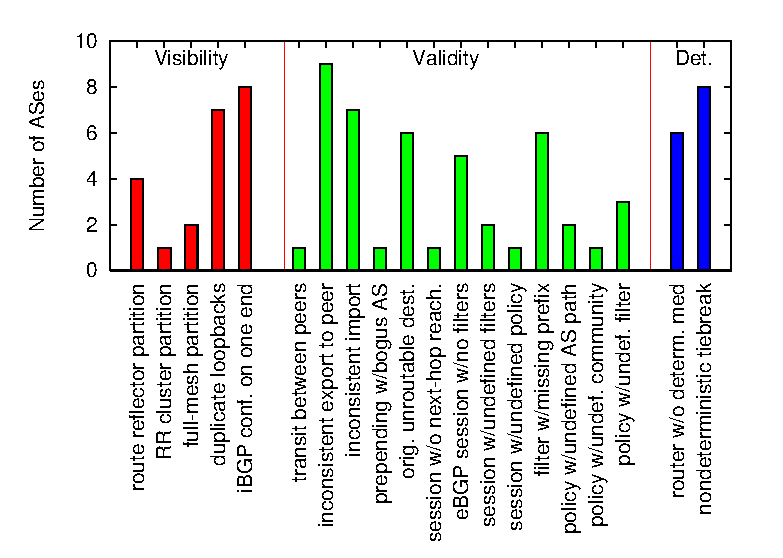
\epsfig{file=rcc/figures/errors_by_as_thesis.eps, width=0.9\linewidth}
\caption{Number of ASes in which each type of fault occurred
  at least once.  
%Unless noted in parentheses, each test was run on all
%  17 ASes.
} 
\label{fig:err_by_as}
\end{figure}



%This example underscores the flexibility
%that operators have in configuring routing protocols and, thus, why
%defining hard and fast correctness rules for BGP is extraordinarily
%difficult.

%% iBGP's goal is simple, but its mechanisms are so complex and obscure
%% that making 
%% mistakes is easy.  We are still discovering
%% configuration subtleties that 
%% fundamentally affect iBGP's correctness.  A replacement for iBGP
%% would eliminate most of these problems.

{\bf Route reflector cluster problems.}  In an iBGP
configuration with route reflection, multiple route reflectors may serve
the same set of clients.  This group of route reflectors and its clients
is called a ``cluster''; each cluster should have a unique ID, and all
routers in the cluster should be assigned the same cluster ID.  If a
router's BGP configuration does not specify a cluster ID, then typically
a router's loopback address is used as the cluster ID.  If two routers
have the same loopback address, then one router may discard a route
learned from the other, thinking that the route is one that it had
announced itself.  \rcc found $13$ instances of routers in distinct clusters
with duplicate loopback addresses and no assigned cluster ID.
%(Table~\ref{tab:errors} shows all cases of duplicate loopback
%addresses, most of which were benign).  
Often, these apparent mistakes may be benign: different physical routers
in the same AS may legitimately have identical loopback addresses.  For
example, routers in distinct IP-layer virtual private networks may route
the same IPv4 address space.


{\bf Incomplete iBGP sessions.} \rcc discovered 420 incomplete iBGP
sessions (\ie, 
a configuration statement on one router indicated the presence of an
iBGP session to another router, but the other router did not have an
iBGP session in the reverse direction).  Many of these faults are likely
benign.  The most likely explanation for the large number of
these faults is that network operators may disable sessions by removing the
configuration from one end of the session without ever ``cleaning up''
the other end of the session.


%\rccns's tests for path visibility in operational networks allowed us to
%discover the following:
%\begin{enumerate}
%\itemsep=-1pt
%\item iBGP configuration is not easy: networks that implemented iBGP
%  with route reflection often had signaling partitions, but \rcc even
%  discovered a small network that had not correctly configured ``full
%  mesh'' iBGP.
%\item Routers occasionally distribute all eBGP-learned routes via IGP,
%  rather than iBGP; in these cases, the fact that a router does not
%  communicate with other routers via iBGP does not matter.
%\item Some aspects of BGP configuration are not maintained or
%  updated as network configuration changes: many configuration files had
%  ``code fragments'' that were vestiges of old BGP sessions but served
%  no function.
%\end{enumerate}

%\rcc also found many instances
%where hundreds of lines of router configuration had been decommissioned.
%In some cases, iBGP sessions (or parts of iBGP sessions) were
%``shutdown'' but remained in the router configuration files.  
%\rcc can
%help operators clean configuration files by highlighting these latent
%faults. 

%%\subsubsection{Route Installation Problems}

%% {\bf Synchronization.}  
%% %Because most ASes only have routers that
%% %participate in iBGP, the configuration option that requires iBGP to be
%% %``synchronized'' with the IGP~(Section~\ref{sec:vis_install}) is usually
%% %disabled.  
%% %Several router vendors disable this option entirely (although
%% %one major vendor still enables the option by default for no good
%% %reason).  
%% We discovered three routers that enabled synchronization; we were unable
%% to contact the operator to find out why 
%% (a vendor provided us with anonymized
%% configurations of one if its customers), but they appeared to be
%% mistakes.  The vendor speculated that their automatic configuration
%% tool may at one time have been configured to enable synchronization by
%% default.

%\item dangling sessions.  things that were established for a specific
%  purpose (\eg, an IETF meeting) and never dismantled afterwards.
%\item duplicate sessions: one to a loopback, one to an interface.
%\item duplicate loopback addresses (\ie, on two different routers)
%\item failure to restore the iBGP mesh after experimentation (ILAN)

%\begin{itemize}
%\itemsep=-1pt
%\item send-community off
%\end{itemize}

%\subsubsection{Anomalies and Curiosities}\label{sec:anomalies}
%Anecdotal stuff.  probably can include stuff here regarding some of the
%  conversations I had with jrex + some ``common nanog knowledge''.  for
%  example,



%interesting
%%  info-flow-control. talk about the DP2AOL community being used to allow
%%  two ``peers'' to use a third ISP for transit.  (note yet
%%  another reason why operators like to keep their configs private)


\subsection{Route Validity Faults}

In this section, we discuss route validity faults.  We first discuss
filtering-related faults; we classify faults as latent unless
a network 
operator explicitly told us that the fault was benign.  
We also describe faults concerning undefined references
to policies and filters.  Some of these faults, while simple to check,
could have serious consequences (\eg, leaked routes), if \rcc had not
caught them and they had been activated.
Finally, we present
some interesting route validity faults related to route dissemination,
all of which 
were benign.  


\subsubsection{Filtering Problems}

Decomposing policies across configurations on different routers can
cause faults, even for relatively simple policies.  \rcc discovered the
following problems: 


{\bf Transit between peers.}  \rcc discovered three instances where
routes learned from one peer or provider could be readvertised to
another; typically, these faults occurred because an export policy for a
session was intended to filter routes that had a certain community
value, but the export policy instead referenced an undefined community.

Obsolete contractual arrangements can remain in configuration long after
those arrangements expire.  \rcc discovered one AS that appeared to
readvertise certain prefixes from one peer to another.  Upon further
investigation, we learned that the AS was actually a previous owner of
one of the peers.  When we notified the operator that his AS was
providing transit between these two peers, he told us, ``Historically,
we had a relationship between them.  I don't know what the status of that
relationship is these days.  Perhaps it is still active---at least in
the configs!''


{\bf Inconsistent export to peer.}  We found $231$ cases where an
AS advertised routes that were not ``equally good'' at every peering
point.  It is hard to say whether these inconsistencies are benign
without knowing the operator's intent, but roughly twenty of these
inconsistencies were certainly accidental. For example, one
inconsistency existed because of an undefined AS path regular expression
referenced in the export policy; these types of inconsistencies have
also been observed in previous measurement studies~\cite{Feamster2004b}.


{\bf Inconsistent import policies.} A recent measurement study observed
that ASes often implement policies that result in late exit (or ``cold
potato'') routing, where a router does not select the BGP route that provides
the closest exit point from its own
network~\cite{Spring2003}.\footnote{Inconsistent import policy technically
  concerns how configuration affects {\em ranking}, and it is more
  often intentional than not.  Nevertheless, this test occasionally highlights
  anomalies that operators are interested in correcting, and it serves
  as a useful sanity check when looking for other types of anomalies (such as
  dynamically detecting inconsistent route advertisements from a
  neighboring AS~\cite{Feamster2004b}).}   \rcc 
found $117$ instances where an AS's import policies explicitly
implemented cold potato routing, which supports this previous
observation.  In one network, \rcc detected a different import policy
for {\em every} session to each neighboring AS. In this case, the import
policy was labeling routes according to the router at which the route
was learned. 

Inconsistent import and export policies were not always
immediately apparent to us upon casual inspection, even after \rcc
detected them. In one case, two 
sessions applied policies with the same name, and both policies were
defined with verbatim configuration fragments.  The difference
resulted from the fact that the difference in policies was three levels
of indirection deep.  For example, one inconsistency occurred because of
a difference in the definition for an AS path regular expression that
the export policy referenced (which, in turn, was referenced by the
session parameters).



%\begin{enumerate}
%\itemsep=-1pt
%% \item BGP configuration often does not follow best common
%%   practices (\eg, filters that reject routes for private or unallocated
%%   prefixes, and deterministic route selection) if the failure to do so
%%   has not yet caused a problem.
%\end{enumerate}

\rcc also detected filtering problems on
single-router configurations:

{\bf Undefined references in policy definitions.} Several large networks
had router configurations that 
referenced undefined variables and BGP sessions that referenced
undefined filters.  
These faults can sometimes result in
unintentional transit or inconsistent export to peers or even potential
invalid route advertisements. 
In one network, \rcc found four routers with undefined filters that
would have allowed a large ISP to accept and readvertise {\em any} route to
the rest of the Internet (such a failure actually occurred in
1997~\cite{www-as7007}, as we described in Section~\ref{sec:intro:problem});
this potentially active fault could have been  
catastrophic if 
a customer had (unintentionally or intentionally) announced invalid routes,
since ASes typically do not filter routes coming from large ISPs.  This
misconfiguration occurred even though the router
configurations were being written with scripts; an operator had
apparently made a mistake specifying {\em inputs} to the scripts.
%These problems mostly seem to surface in configurations where
%operators said they were frequently changing settings.


{\bf Non-existent or inadequate filtering.}  
%As we described in
%Section~\ref{sec:val_filters}, correct filtering practices do not
%guarantee validity, but they certainly prevent obviously invalid routes
%from propagating.  Missing or incorrect import filters can result in
%invalid routes being propagated within an AS and advertised to other
%ASes.  
Filtering can go wrong in several ways: (1)~no filters are used
whatsoever, (2)~a filter is specified but not defined, or
(3)~filters are defined but are missing prefixes or otherwise
out-of-date (\ie, they are not current 
with respect to the list of private and unallocated IP address
space~\cite{www-cymru-bogon}). 

Every network that \rcc analyzed had faults in filter configuration.
Some of these faults would have caused an AS to readvertise {\em any}
route learned from a neighboring AS.  In one case, policy
misconfiguration caused an AS to transit traffic between two of its
peers.  Table~\ref{tab:errors} and Figure~\ref{fig:err_by_as} show that
these faults were extremely common: \rcc found 21 eBGP sessions in 5
distinct ASes with no filters whatsoever and 27 eBGP sessions in 2 ASes
that referenced undefined filters.  Every AS had partially incorrect
filter configuration, and most of the smaller ASes we analyzed either
had minimal or no filtering.  Only a handful of the ASes we analyzed
appeared to maintain rigorous, up-to-date filters for private and
unallocated IP address space.  These findings agree with those of our
recent measurement study, which also suggests that many ASes do not
perform adequate filtering~\cite{Feamster2004f}.

%We wondered why filtering practices were so poor.  
The reason for inadequate
filtering seems to be the lack of a process
for installing and updating filters. 
One operator told us
that he would be willing to apply more 
rigorous filters if he knew a good way of doing so.  Another operator runs
sanity checks on filters and was surprised to find that many
sessions were referring to undefined filters.   
Even a well-defined process can go horribly wrong: one operator intended
to use a 
feed of unallocated
prefixes to automatically install filters, but instead ended up
readvertising them.
Because there is a set of prefixes that every AS should always filter,
some prefixes should be filtered by default.  
%Another possibility is to
%build validity checks into 
%BGP itself~\cite{kent2000b,Subramanian2004}.



\subsubsection{Dissemination Problems}

\rcc found only benign faults involving dissemination.

{\bf Unorthodox AS path prepending practices.}  An AS will often prepend
its own AS number to the AS path on certain outbound advertisements to
affect inbound traffic.  However, we found one AS that prepended a
neighbor's AS on {\em inbound advertisements} in an apparent attempt to
influence {\em outbound traffic}. One network operator also mentioned
that ASes sometimes prepend the AS number of a network that they want to
prevent from seeing a certain route (\ie, by making that AS discard the
route due to loop detection), effectively ``poisoning'' the route.  We
did not witness this poisoning in any of the configurations we analyzed.

{\bf iBGP sessions with ``next-hop self''.}  We found two cases of iBGP
sessions that violated common rules for setting the next-hop
attribute, both of which were benign.  First, \rcc detected
route reflectors that appeared to be setting the ``next hop''
attribute. Although this practice is not likely to create active faults,
it seemed unusual, since the AS's exit
routers typically set the next-hop IP address, and route reflectors
typically do not modify route attributes.
Upon further investigation, we learned that some router vendors do not
allow a route reflector to reset the next-hop attribute. Even though
the configuration specified that the session would reset the next-hop
attribute, the configuration statement had no effect because the
software was designed to ignore it. The operator who wrote the
configuration specified that the next-hop attribute be reset
on these sessions to make the configuration appear more uniform.
Second, routers sometimes reset the
next-hop on iBGP sessions to themselves on sessions to a route
monitoring server to allow the
operator to distinguish which router sent each route to the monitor.


\subsection{Determinism Faults}

\rcc discovered more than two hundred routers that were
configured such that the arrival order of routes affected the outcome of
the route selection process (\ie, these routers had either one or both of
the two configuration settings that cause nondeterminism).  Although
there are occasionally reasonably good reasons for introducing ordering
dependencies (\eg, preferring the ``most stable'' route; that is, the
one that was advertised first), operators did not offer good reasons for
why these options were disabled.  In response to our pointing out this
fault, one operator told us,``That's a good point, but my network isn't
big enough that I've had to worry about that yet.''  
%Many operators either are unaware of or indifferent to the benefits of
%determinism.  
Nondeterministic features should be disabled by default.



%\rcc detected hundreds of instances where a router would attempt to
%originate a prefix via eBGP but would have no route to that prefix.
%Because BGP will not advertise any prefix for which it does not have a
%route, these instances should be removed from configuration.


%% \begin{figure}[ht!]
%% \centering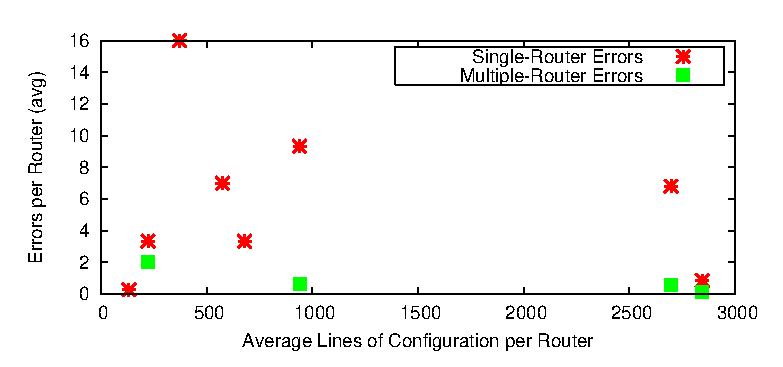
\epsfig{file=rcc/figures/errors_by_loc.eps, width=\linewidth}
%% \caption{Average number of errors per router in an AS vs. the median lines of
%%   configuration for routers in that AS.}
%% \label{fig:errors_by_loc}
%% \end{figure}

%\subsubsection{Effects of Network Size}

%To explore how complexity affects the prevalence of errors in router
%configuration, we examined whether the configuration errors in a network
%are relatively more prevalent in larger networks.  One might expect
%that ASes with larger configuration files, more routers, or more
%sessions might have proportionally more errors. 
%This agrees with our observation
%that errors result from the lack of a systematic process for configuring
%routers, too many levels of indirection, and the fact that the protocol
%itself is so complex that there is little understanding of correct
%configuration in the first place.  These phenomena are true regardless
%of the size or complexity of the AS.
%Figure~\ref{fig:errors_by_loc} shows, for each AS that we had access to
%router configurations, the average number of errors per router in that
%AS vs. the median number of lines of configuration in a router
%configuration in that AS.%\footnote{Median lines of configuration seemed
%to be a better indicator of complexity for BGP configurations than
%average.  Several ASes had many routers with relatively small
%configurations and one or two routers with routers that had
%configurations several orders of magnitude larger.}  
%We consider configuration errors that involve a single router
%(``single-router errors'') separately from errors that involve
%configurations across multiple routers (``multiple-router errors'').


%% \subsection{Prevalence of Anomalies and Errors}

%% Frequency of various types of anomalies.  I think basically we want to
%% say either (1)~we saw this happen in practice (say whether it was once
%% onr ``multiple times''), (2)~we didn't see this, but operators say
%% anecdotally that this type of thing happens frequently.

%% \begin{itemize}
%%         \item whether we tested it (most of these should be "yes")
%%         \item whether it occurred in the configs we saw
%% \begin{itemize}
%%                 \item if so, did it occur multiple times (\ie, in different
%%                   configs for the same AS, in configs in multiple ASes,
%%                   etc.)
%%                 \item if not, whether it occurs "anecdotally" (\ie, does
%%                   Avi Freedman or Randy Bush, etc., say it happens, or has
%%                   the problem been discussed on nanog, been in popular
%%                   press, etc.)
%% \end{itemize}
%%         \item whether the problem should be fixed by:
%% \begin{itemize}
%%                 \item config language fix
%%                 \item protocol fix
%%                 \item decision process fix
%%                 (or some combination)
%% \end{itemize}
%% \end{itemize}





\section{Take-away Lessons}\label{sec:rcc_lessons}


In recent years, much work has been done to understand BGP's
behavior, and much has been written about the wide range of problems it
has.  Some argue that BGP has outlived its purpose and should be
replaced; others argue that faults arise
because today's configuration languages are not
well-designed.  We believe that our evaluation of faults in
today's BGP configuration provides a better understanding of the
types of errors that appear in today's BGP configuration and the
problems in today's configuration languages.  
%
%Our evaluation of real-world BGP configuration from operational networks
%suggests several higher-level lessons about the nature of today's
%configuration process.  
We now briefly explore how our findings may help inform the design
of Internet routing systems in the future.

First, operational networks---even large, well-known, and well-managed
ones---have faults.  Even the most competent of operators find it
difficult to manage BGP configuration.  In particular, iBGP is
misconfigured often.  In fact, in the absence of a guideline such as
Theorem~\ref{thm:vis}, it is hard for a network operator to know what
properties the iBGP signaling graph should have.  Ideally, network
operators should be able to configure an AS without having to worry
about whether these types of constraints are satisfied in the first
place; in other words, a network operator should not be allowed to
express a configuration that violate properties such as path visibility
and route validity.  In Chapter~\ref{chap:concl}
(Section~\ref{sec:rcp}), we discuss a system for disseminating BGP
routes within an AS called the Routing Control Platform
(RCP)~\cite{caesar2004,feamster:fdna2004}, which could explicitly
enforce properties such as route validity and path visibility.

%
Second, we found that route filters are poorly maintained.  Routes that
should never be seen on the global Internet (\eg, routes for private
addresses) are rarely filtered, and the filters that are used are often
misconfigured and outdated.  We can make significant strides towards
fixing these types of problems simply by changing the default behavior
of router filters.  For example, because private address space (\ie, as
specified in RFC 3330~\cite{rfc3330}) should not be advertised on the
global Internet, routers could, by default, prevent routes for this
address space from leaking across AS boundaries.  Of course, network
operators who required routes for this address space to be advertised
across AS boundaries (\eg, in cases where a single administrative domain
comprises multiple ASes) could configure that behavior as an {\em
exception}, but the default behavior would reduce the likelihood of
erroneous route leaks.

%
Third, the majority of the configuration faults that \rcc detected
resulted from the fact that an AS's configuration is distributed across
its routers.  Maintaining network-wide policy consistency appears to be
difficult; invariably, in most ASes there are routers whose
configuration appears to contradict the AS's desired policy.  A routing
architecture or configuration management system that enabled an operator
to configure the network from a centralized location with a high-level
language would likely prevent many serious faults.

%
Finally, although operators use tools that automate some aspects of
configuration, these tools are not a panacea.  In fact, we found cases
where the incorrect use of these tools {\em caused} configuration
faults.  This observation suggests that static configuration
analysis will play an important role in the configuration
workflow, regardless of future improvements in configuration languages
or routing architectures.  As long as the routing protocol offers
flexible configuration, the potential for incorrect behavior exists.
Our work has demonstrated that detecting incorrect behavior {\em
proactively} using static configuration analysis is not only
surprisingly effective, but it is also necessary for detecting faulty
configurations before they introduce erroneous behavior on a live
network. 



\section{Summary}
\label{s:rcc_concl}


Despite the fact that BGP is almost 10 years old, operators continually make
the same mistakes as they did during BGP's infancy.   Our work takes a
step towards improving this state of 
affairs by making the following contributions:
%\vspace*{-0.05in}
\begin{itemize}
\itemsep=-1pt
%\item We define a high-level correctness specification for BGP and
%  map that specification to conditions that can be tested with static
%  analysis.
\item We use the correctness specification from Chapter~\ref{chap:rlogic}
  to design and implement 
  \rccns, a static analysis tool that detects faults by analyzing the
  BGP configuration across a single AS.  With \rccns, network operators
  can find many faults {\em before} deploying configurations in
  an operational network.  \rcc has been downloaded by over seventy network
  operators.
\item We use \rcc to explore the extent of real-world BGP
      misconfigurations.  We have analyzed
      real-world, deployed configurations from 17 different ASes and
      detected more than 1,000 BGP configuration faults that had
      previously gone undetected by operators.
\end{itemize}



%framework to the design and implementation of \rccns, a tool that uses
%static analysis to verify BGP configuration correctness.  Our tool has
%helped operators debug real-world BGP configuration.  Third, we
%present our findings on BGP configuration errors and anomalies from
%static analysis of real-world BGP configurations.  This paper is the
%first to explore BGP configuration errors using analysis of real-world
%BGP configuration files.  Finally, we suggest concrete ways to improve
%BGP's correctness, distinguishing problems that should be fixed with
%protocol modifications from those that should be fixed with a better
%configuration language.

In light of our findings, we suggest two ways to make interdomain
routing less prone to configuration faults.  First, protocol
improvements, particularly in intra-AS route dissemination, could avert
many BGP configuration faults.  The current approach to scaling iBGP
should be replaced.  Route reflection serves a single, relatively simple
purpose, but it is the source of many faults, many of which cannot be
checked with static analysis of BGP configuration
alone~\cite{Griffin2002}.  The protocol that disseminates BGP routes
within an AS should enforce path visibility and route validity; the
Routing Control Platform offers one possible solution.

Second, BGP should be configured with a centralized, higher-level
specification language.  Today's BGP configuration languages enable an
operator to specify router-level {\em mechanisms} that implement
high-level policy, but the distributed, low-level nature of the
configuration languages introduces complexity, obscurity, and
opportunities for misconfiguration rather than design flexibility or
expressiveness.  For example, \rcc detects many faults in implementation
of some high-level policies in low-level configuration; these faults
arise because there are many ways to implement the same high-level
policy, and the low-level configuration is unintuitive.  Ideally, a
network operator would never touch low-level mechanisms (\eg, the
community attribute) in the common case.  Rather than configuring
routers with a low-level language, an operator should configure the {\em
network} using a language that directly reflects high-level
policies.



%, and this specification could be ``compiled'' into
%configuration statements that implement the policies.
% (Such a specification would also be much easier to analyze
%with a tool like \rccns.)



%XXX FUTURE WORK: IGP/iBGP...

%% The hard stuff, like iBGP, isn't going to get better.  Same with things
%% like MED osc.  For these, we need protocol changes.  This is part of our
%% ongoing work (\eg, route servers to impose a total ordering, scrap iBGP
%% to avoid partitions, guarantee consistent export, etc.)

%% Same thing with safety.  It's fundamental to the protocol (Arrow's
%% impossibility thm), and protocol changes must happen to solve this
%% problem correctly.

%% For other stuff that people mess up, we need better interfaces.  These
%% interfaces should reflect that there are only a handful of tasks that
%% operators need to perform.


% Herb Caen:  "The clock doesn't matter in baseball. Time stands still or moves backwards. Theoretically, one game could go on forever. Some seem to."

%"Slow it down to stay ahead of it to stay on top of it." -Tony LaRussa

%"There are three types of baseball players: those who make it happen,
%those who watch it happen, and those who wonder what happens." - Tommy Lasorda

%Abbott: Now, on the St. Louis team we have Who's on first, What's on
%second, I Don't Know is on third. Costello: That's what I want to find
%out.

% I say Who's on first, What's on second, I Don't Know's on third.
%- Lou Costello 


\qchapter{\textit{There are three types of baseball players: those who
make it happen, \\ those who watch it happen, and those who wonder what
happens.} \vskip 0.1em - Tommy Lasorda}{Predicting BGP Routes with
Static Analysis}\label{chap:sandbox}

%%%
%%% introduction.tex
%%%

%\section{Introduction}
\label{sec:sandbox_intro}
%%%
%%% Operators needs models or their heads will explode
%%%
\cs{T}o~~control the flow of traffic through their networks, operators need
to know how configuration changes affect the routes that each router in
the network selects.  The outcome of this route selection depends on the
routes advertised by neighboring domains, the internal topology, the
interdomain routing policies, and the intradomain link weights.  To
avoid costly debugging time and catastrophic mistakes, operators must be
able to quickly predict the routes that each router selects.  Our
approach to solving this problem is to develop a network-wide model of BGP
route selection that enables fast, efficient computation of these
routes. In this chapter, we present efficient algorithms for computing
the routing decision at each router in an AS.  Ordinarily, such
computation would require a complex simulation of routing protocol
dynamics that might not reflect the outcome on a live network anyhow if
the routing system oscillates or has multiple stable outcomes.  Using
the correctness specification from Chapter~\ref{chap:rlogic} and a tool
like \rcc (Chapter~\ref{chap:rcc}) to check that the properties of the
correctness specification hold, however, we can exploit the fact that a
routing protocol that satisfies some of these properties makes computing
the network-wide outcome of BGP route selection much simpler.

In designing these route prediction algorithms, we grapple with two
features of the BGP: violations of determinism
(Definition~\ref{def:determinism}), and limited visibility into the
available routes for each destination.
%
%This chapter uses a model of BGP route selection inside a single AS to
%develop algorithms that efficiently compute the outcome of BGP route
%selection at each router.  
This chapter presents three main contributions.

\begin{enumerate}
\itemsep=-1pt
\item \textbf{Algorithms for predicting BGP route selection.}
Rather than analyzing BGP {\em dynamics}, we present efficient
algorithms to compute the outcome of the distributed route-selection
process using only {\em static} inputs.  Our algorithms exploit the
following observation: when a routing system converges, the outcome does not
depend on the order and timing of the messages, allowing our algorithms
to model a message ordering that efficiently computes the outcome of BGP
route selection.

Section~\ref{sec:setup} presents practical constraints that enable
efficient computation of network-wide BGP route selection 
and describes an overview of the algorithms presented in the rest of the
chapter.  After we introduce some notation (Section~\ref{sec:basic}),
Section~\ref{sec:egress_set} presents an algorithm that computes the
outcome of BGP route selection for the simple case where every router in
the AS receives every router's best eBGP-learned route for a destination
(which corresponds to a full mesh iBGP configuration) and where
determinism is satisfied (which 
corresponds to a routing protocol where all route attributes can be
compared across all routes; \ie, without MED\footnote{Throughout the
chapter, we often describe BGP ``without MED''. Network configurations
``without MED'' could also be viewed as a configuration that compares
the MED attributes across all routes (\eg, in Cisco IOS, this behavior
can be enabled with {\tt always-compare-med} setting).}).  This
algorithm turns out to be quite simple.  

The balance of the chapter
deals with route prediction in networks that employ MED, route
reflection, or both.
We first present algorithms that handle MED
and route reflectors in isolation.  We then discuss why the interaction
between these two features precludes efficient route prediction.
Section~\ref{sec:med_model} focuses on algorithms that capture the
effects of the MED attribute, assuming a full-mesh iBGP configuration.
In Section~\ref{sec:best_egress}, we consider iBGP configurations that
use route reflection.

\item {\bf Prototype implementation.}
We describe a prototype implementation of a tool based on our prediction
algorithms.  This tool provides fast, accurate answers to ``what if''
questions about the effects of configuration changes on the flow of
traffic through the network.  We tested this prototype on a large tier-1
ISP to demonstrate that our prediction algorithms are fast and accurate
enough to be used in practice.  Section~\ref{sec:sandbox_implementation}
summarizes the design, evaluation, and validation of this
tool~\cite{Feamster2004}.

\item \textbf{Proposed improvements to BGP.} 
Two features---the MED attribute and route reflection---complicate route
prediction and create difficulties for the operation of BGP itself.
Section~\ref{sec:discussion} suggests ways to improve the design and
operation of BGP to avoid the harmful effects without sacrificing the
policy semantics of MEDs and the scalability provided by route
reflectors.
\end{enumerate}


%\subsection*{Backbone Network Engineering}
%%%
%%% eBGP and iBGP
%%%
\section{Motivation and Overview}

This section briefly reviews the BGP route selection process
(Table~\ref{tab:background:decision} and
Section~\ref{sec:bg:route_selection} provide coverage in greater 
depth) and discusses why network operators need algorithms to
efficiently compute the outcome of this route selection process.

Recall from Section~\ref{sec:bg:route_selection} that the route selected
by each router depends on the interactions between three routing
protocols, as shown in Figure~\ref{fig:example}.  First, routers in the
AS use {\em external BGP (eBGP)} to receive route advertisements from
neighboring ASes.  For example, the routers $W$, $X$, and $Y$ each have
eBGP sessions with neighboring ASes.  As described in
Section~\ref{sec:semantics}, to influence the route selection process,
a router may apply an {\em import\/} policy to modify the attributes of
the routes learned from a neighbor.

Second, the routers use {\em internal BGP (iBGP)} to disseminate the routes to
the rest of the AS.  In the simplest case, each router has an iBGP
session with every eBGP-speaking router, forming an ``full mesh''
configuration.  If two routes are equally good through the first four
steps in Table~\ref{tab:background:decision}, the router favors an
eBGP-learned route over an iBGP-learned one.  In
Figure~\ref{fig:example}, router $Z$ receives three iBGP routes, from
routers $W$, $X$, and $Y$. If the routes that $Z$ learns have equal
local preference, AS path length, origin type, and MED values, it uses
the IGP to break ties between the remaining
routes~\ref{tab:background:decision}.

Third, the routers run an Interior Gateway Protocol (IGP) to learn how
to reach each other.  Two common IGPs today are OSPF~\cite{rfc1583} and
IS-IS~\cite{rfc1142}, which compute shortest paths based on configurable
link weights; the routers also use the IGP path costs in the sixth step
in Table~\ref{tab:background:decision}.  In Figure~\ref{fig:example},
router $Z$ selects the route with the smallest IGP path cost of $2$,
learned from router $X$.\footnote{If two routes have the same IGP path
cost, the router performs an arbitrary tiebreak in the seventh step in
Table~\ref{tab:background:decision}.}

After selecting a route to each destination, each router combines the
BGP and IGP information to construct a forwarding table that maps the
destination prefix to the outgoing link along the shortest path.  In
Figure~\ref{fig:example}, the forwarding path consists of the thick
lines from the ingress link at router $Z$ to the egress link at router
$X$.

\begin{figure}
\begin{center}
\begin{psfrags}
\psfrag{W}{$W$}
\psfrag{X}{$X$}
\psfrag{Y}{$Y$}
\psfrag{Z}{$Z$}
\psfrag{I}{$I$}
\psfrag{AS A}{{\Large AS $A$}}
\psfrag{AS B}{{\Large AS $B$}}
\resizebox{0.4\linewidth}{!}{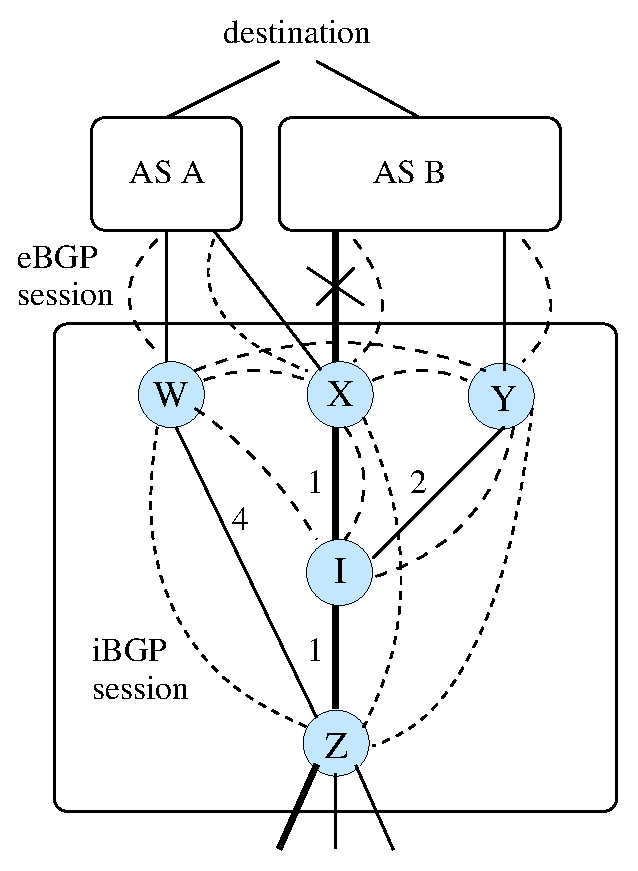
\includegraphics{sandbox/figures/tweak.eps}}
\end{psfrags}
\end{center}
\caption[Network with three egress routers connecting to two neighboring
ASes]{Network with three egress routers connecting to two neighboring
ASes: Solid lines correspond to physical links (internal links are
annotated with IGP link weights) and dashed lines correspond to BGP
sessions.  Thick lines illustrate the shortest path from one router to
its closest egress point for reaching the destination.} 
\label{fig:example}
\end{figure}


%%%
%%% Tweaking policy
%%%
If the link from $X$ to AS $B$ becomes persistently congested, the
network operator may need to adjust the configuration of the routing
protocols to direct some of the traffic to other egress routers.  For
example, the operator could modify the import policy at router $X$ for
the routes it learns from AS $A$ and AS $B$ to make the BGP routes for
some destinations look less attractive than the routes received at other
routers~\cite{Feamster2003e}.  Changing the import policy in this way
causes the route that $X$ readvertises via iBGP to carry a smaller {\em
local preference\/}, which influences the routes that other routers
in the network select.  For example, changing the import policy at $X$
has the {\em indirect\/} effect of directing some of the traffic
entering at router $Z$ to egress router $Y$ (the next-closest egress
point, in terms of the IGP path costs), thereby alleviating the
congestion on the link connecting $X$ to AS $B$.  Network operators make
similar kinds of configuration changes for a variety of other reasons, such
as exploiting new link capacity, preparing for maintenance on part of
the network, or reacting to equipment failures.

Operators must predict the effects of changes to the routing protocol
configuration before modifying the configuration on a live network.
Human intuition is not sufficient for understanding the complex
interactions between three routing protocols running on a large, dynamic
network.  Experimenting on a live network runs the risk of making
disruptive configuration changes that degrade performance.  Instead, we
believe that operators should have an accurate and efficient tool that
computes the effects of configuration changes on the flow of traffic
through the network.  This tool should allow a network operator (or an
automated optimization algorithm) to efficiently explore the large space
of possible configurations.

\section{Problem Statement and Challenges}\label{sec:sb_challenges}

Our goal is to compute the {\em outcome\/}---the routing decision for
each router---once the routing protocols have converged.  Accordingly,
we present algorithms that accurately and quickly determine how the
network configuration and the routes learned via eBGP affect the flow of
traffic through an AS.  While some existing tools simulate BGP's
behavior~\cite{www-ns-bgp,www-cbgp,www-ssfnet}, this work is the first
to develop algorithms that determine the outcome of the BGP route
selection process at each router in an AS without simulating the
dynamics of the protocol.

Efficiently predicting the route that each router in an AS ultimately
selects is challenging because the route selected by one router often
depends on the routes selected by other routers in the AS.  Consider
Figure~\ref{fig:simple}. In this example, router $R_1$ receives two
routes via eBGP, while $R_2$ receives a single route via eBGP.  To
determine the route that each one of these routers ultimately selects,
we must first determine the candidate routes available to each router.
Of course, the set of candidate routes available to each of these routers
depends on the route that the other selects!  This circular dependency
seems to imply some ``back and forth'' reasoning (\ie, determining the
route that $R_1$ selects depends on the route that $R_2$ selects, which
in turn depends on the route that $R_1$ selects, etc.).  Efficiently
resolving these types of circular dependencies is the focus of this
chapter.
%
\vspace{0.15in}
\begin{center}
\framebox{
\noindent
\parbox{0.85\linewidth}{
{\bf Problem:} Given only a static snapshot of the routing configuration
for the routers in an AS and the eBGP-learned routes received by the
routers in the AS, determine the route that each router in an AS selects
for each destination, while considering each AS's available candidate
routes only once. 
}
}
\end{center}
\vspace{0.15in}


\begin{figure}
\begin{center}
\begin{psfrags}
\psfrag{R_1}{{\LARGE $R_1$}}
\psfrag{R_2}{{\LARGE $R_2$}}
\psfrag{a}{{\LARGE $a$}}
\psfrag{b}{{\LARGE $b$}}
\psfrag{c}{{\LARGE $c$}}
\resizebox{0.6\linewidth}{!}{\includegraphics{sandbox/figures/simple.eps}}
\end{psfrags}
\end{center}
\caption[Route prediction requires resolving circular
dependencies.]{Route prediction requires resolving circular
dependencies.  Determining the route that $R_2$ ultimately selects (\ie,
$a$, $b$, or $c$) first requires determining whether $R_1$ selects route
$a$ or $b$.  Ultimately, $R_1$'s selected route could depend on whether
it learns route $c$ from $R_2$, which requires revisiting $R_1$.
}
\label{fig:simple}
\end{figure}

\noindent
Solving this problem would be easy if (1)~the decision process in
Table~\ref{tab:background:decision} allowed each router to form a
ranking of the candidate routes that satisfied determinism
(Definition~\ref{def:determinism}); and (2)~the dissemination of routes
in iBGP ensured each router received the best route for a destination
from every eBGP-speaking router.  If these two properties held, then a
simple algorithm that simply considered which route each router would
select from all of the eBGP-learned routes would correctly compute the
outcome of BGP route selection without having to revisit any routers.
Unfortunately, two features of BGP cause these properties to be
violated, thus making route prediction more challenging:

First, {\bf in practice, each router's ranking function violates
determinism}; the violation is caused by BGP's MED attribute.  An eBGP
neighbor can set the MED attributes of route advertisements on different
BGP sessions to influence the behavior of the routers that receive these
routes in a neighboring AS.  For example, in Figure~\ref{fig:example},
AS $B$ may send a route with a MED of $10$ to router $Y$ and a route
with a MED of
$20$ to router $X$;
% in order to receive traffic to the destination through router $Y$.
as a result, $Z$ would select the route from $Y$ with the smaller MED,
even though the IGP path to $X$ is shorter.  The MED comparison in
step~$4$ of the decision process applies only to routes learned from the
{\em same} next-hop AS.  When MEDs are used in this fashion, however, each
router's ranking function violates determinism (see
Figure~\ref{fig:determinism_bgp}). In other words, the choice of one route over
another may depend on the presence or absence of a third
route~\cite{www-cisco-determed}.

In Chapter~\ref{chap:rlogic}, we described how violations of determinism
can cause safety problems.  Determinism problems also complicate route
prediction, because each router's rankings among a set of candidate routes
may depend on the routes that other routers in the network select.  An
efficient route prediction algorithm must resolve these dependencies. 

Second, {\bf routers in an AS may not receive every eBGP-speaking
router's best route for a destination}. The quadratic scaling of a
full-mesh iBGP configuration forces large networks to distribute routes
in a hierarchical fashion.  A router configured as a route reflector
selects a single best route and forwards the route to its clients (see
Section~\ref{sec:dissemination} for details).
Using route reflectors reduces the number of iBGP sessions, as well as
the number of routes the clients need to receive and store.  Because
each route reflector forwards only its {\em best} route to its iBGP
neighbors, however, the candidate routes available at one router depend
on decisions at other routers.  In particular, a route reflector may
make a different choice in step~6 of the route selection process (\ie,
shortest IGP path to the next-hop IP address) than its clients would
have because it is 
located at a different place in the IGP topology than its clients.

In general, these two features of BGP cannot be ignored because
operators use them often.  To illustrate the extent to which these
artifacts of BGP complicate route prediction, we present the ``ideal''
route prediction algorithm in Section~\ref{sec:egress_set}, before
considering more complicated algorithms that capture the effects of
these two artifacts.
% to provide flexibility and scalability, respectively.

%%%
%%% Contributions
%%%

%%%
%%% setup.tex
%%%


\section{Modeling Constraints and Algorithm Overview}
\label{sec:setup}
%%%
%%% Introduction
%%%
In this section, we impose three constraints that the routing system
must satisfy to enable efficient and accurate route prediction.  

Next, we describe how these constraints enable us to decompose the
algorithm into three stages---applying the import policy to eBGP-learned
routes, selecting the best BGP route at each router, and computing the
forwarding path.  The algorithm takes as input the router configuration
and a static snapshot of the routes learned via eBGP and outputs the
route that each router in the AS selects, for each destination.  Because
the first and third stages of the algorithm are relatively simple, the
rest of the chapter focuses on the second stage of computing the best
BGP route at each router for each destination prefix.



\subsection{Modeling Constraints}
%%%
%%% Feasibility of such a model
%%%
Efficiently computing the effects of a configuration or topology change
is possible 
when three important conditions hold.  These constraints include the
various correctness properties specified in
Chapter~\ref{chap:rlogic} that can be verified with static configuration
analysis (Chapter~\ref{chap:rcc}).  Specifically, we assume that safety,
and the second condition of determinism are satisfied.  Imposing these
constraints free our prediction algorithms from needing to consider
whether different orderings of routing will produce different results.
This property allows us to focus on designing algorithms that emulate a
particular message ordering that prevents the algorithm from having to
revisit routers where it has already made a prediction.  The rest of
this section explains how these constraints and others help simplify the
prediction algorithms.

First, the inputs to the algorithm must be stable.  In particular,

\begin{constraint}[Slowly changing inputs]
\label{a:ebgp}
The eBGP-learned routes change slowly with respect to the timescale of
network engineering decisions.
\end{constraint}

\vspace*{0.1in}
\noindent
If the eBGP-learned routes change frequently, the internal routing
system does not have time to propagate the effects of one eBGP
advertisement before the next one arrives.  In practice, most BGP
routes are stable for days or weeks at a time~\cite{labovitz99}, and
the vast majority of traffic is associated with these stable
routes~\cite{Rexford:stability2002}.  This allows the routing algorithm to operate on
a static snapshot of the eBGP routes.  Any eBGP routing change can be
treated as a separate problem instance.

Second, the routers in the AS must ultimately reach a stable
outcome.  In particular,

\begin{constraint}[Safety and uniqueness]
\label{a:ibgp}
Given stable eBGP-learned routes and fixed iBGP and IGP topologies,
each router inside the AS converges to a unique routing decision.
\end{constraint}

\vspace*{0.1in}
\noindent
If the routers continually change the routes that they select,
accurately predicting how the flow of data traffic becomes significantly
more challenging.  Fortunately, previous work~\cite{Griffin2002} has
identified sufficient conditions for an internal routing configuration
to satisfy Constraint~\ref{a:ibgp}.  We describe these conditions in
more detail in Section~\ref{sec:best_egress} when we address the
challenges introduced by route reflectors.

Third, the routing decisions at each router should not depend on
message ordering or timing:

\begin{constraint}[Determinism, Condition \#2]
\label{a:determ}
The routing decision at each router depends only on the routes received
from its neighbors and {\em not} the order or timing of these routing
messages. 
\end{constraint}

\vspace*{0.1in}
\noindent
Some router vendors have an additional step in the BGP
decision process that favors the ``oldest'' route before the final
tie-breaking step of comparing the router IDs.  The ``age-based
tie-breaking'' favors more stable routes, making the outcome of the
BGP decision process dependent on the {\em order\/} the router
receives the advertisements (and, hence, violating determinism).
Disabling age-based tie-breaking forces 
a deterministic selection based on the smallest router ID, as in
Figure~\ref{tab:background:decision}; other BGP features, such as route flap
damping~\cite{rfc2439}, can help reduce the likelihood of selecting
unstable routes.


Constraint~\ref{a:ibgp}, which guarantees that the routing system will
converge to a unique outcome, and~\ref{a:determ}, which guarantees that
this outcome does not depend on the ordering of routing messages, allow
us to make the following observation:

\vspace{0.15in}
\begin{center}
\framebox{
\parbox{0.85\linewidth}{
\begin{observation}
\label{t:order}
If a routing system is guaranteed to converge to a unique outcome,
that outcome is independent of the order in which routers exchange routes
and apply the decision process.
\end{observation}
}
}
\end{center}
\vspace*{0.1in}
\noindent
This observation implies that the algorithm can consider the evolution
of the routing system under {\em any particular message ordering},
without the risk of arriving at the wrong answer.

%% note the properties that the algorithms do {\em not} require

It is worth noting that our algorithms do not require the routing system
to satisfy route validity or the first condition of determinism (recall
that determinism is only a sufficient condition for iBGP to satisfy
safety but is not necessary).  The algorithms in this chapter are only
concerned with predicting the outcome of BGP selection process, not
whether the resulting routes induce paths that violate route validity.  In
Sections~\ref{sec:med_model} and~\ref{sec:best_egress}, we permit
routers' selection functions to violate the first condition of
determinism because these violations capture BGP's default behavior
(\ie, this condition is violated whenever routers only compare the MED
attribute across routes received from the same neighboring AS).  The
algorithms do not explicitly require path visibility; rather, the
algorithms in
Sections~\ref{sec:simple} and~\ref{sec:med_model} implicitly assume path
visibility is satisfied (\ie, they assume a ``full mesh'' iBGP
configuration).

\subsection{Overview: Decomposing BGP Route Selection into Three
  Stages}\label{sec:decompose} 

\begin{figure*}
\centering\epsfig{file=sandbox/figures/bigpic4.eps,width=\textwidth}
\caption[Decomposing BGP route selection into three
  independent stages.]{Our algorithms decompose network-wide BGP route
  selection into three independent stages.  The algorithms take as input
  the eBGP-learned routes from neighboring ASes, the router IDs of each
  BGP session, and the routing configurations from all of the routers in
  the AS, which provide information about the IGP topology, the iBGP
  topology, and the import policies (\ie, rankings) of each router.}
\label{fig:modules}
\end{figure*}

Following the approach applied in other recent
work~\cite{Feamster2005b,Gao2001a}, the algorithms in this chapter
compute the effects of a particular message ordering using an {\em
activation sequence\/}, an {\em offline} analysis technique that
``activates'' one or more routers at each discrete step.  When
activated, a router applies the decision process in
Table~\ref{tab:background:decision} and propagates the best route to its
iBGP neighbors.  Our algorithms are based on an activation sequence that
allows us to decompose route prediction into three distinct stages, as
shown in Figure~\ref{fig:modules}:

\textbf{1. Receiving the eBGP routes and applying import policy.} This
stage takes as input all of the eBGP-learned routes at each router and
applies the appropriate import policies at each router {\em before
exchanging any iBGP update messages} and outputs the set of eBGP-learned
routes after these import policies have been applied.  This stage
activates all of the edge routers at the same time.  

Each eBGP-learned route has attributes (such as the destination prefix
and the AS path) and is associated with an eBGP session.  The import
policy may filter the route or set certain attributes such as local
preference, origin type, and multiple-exit discriminator (MED),
according to attributes in the advertised route (\eg, based on ASes in
the AS path).  Because applying the import policy is a local operation
for each eBGP-learned route at each router, the first stage emulates the
operations a real router would perform upon receiving each of the eBGP
routes.  These routes, with modified attributes, are the input to the
second stage.

\textbf{2. Computing the best BGP route at each router.}  When iBGP
satisfies path visibility, many routes from the first stage could never
be selected by any router as the best route.  For example, an
eBGP-learned route with a local preference of 90 would {\em never} be
selected over another route with a local preference of 100.  In
addition, different routers in the AS may select different best BGP
routes because they have different IGP path costs to the egress router.
Also, a router can only consider the routes advertised by its iBGP and
eBGP neighbors, which may influence the final decision at that router.
%Deriving accurate and
%efficient algorithms for computing the best BGP route at each router
%is the main contribution of this paper.  
This stage takes as input the set of eBGP-learned routes after the
import policies of each router have been applied and outputs a single
best egress router for each ingress router and destination prefix.
Constructing an efficient activation sequence for this stage is
challenging, and is the focus of the next four sections of the chapter.

Using Observation~\ref{t:order}, our goal is to devise an {\em
activation sequence\/}, which ``activates'' one or more routers at any
given phase.  When activated, a router $r$ applies the BGP decision
process to compute a best route from its available candidate routes,
which it then may propagate to other routers via iBGP.  In an actual
network, routers may be activated in any order and may change their best
route many times before the network converges.  This chapter focuses on
devising activation sequences that allow us to efficiently compute
the final routing decision.


\textbf{3. Computing the forwarding path through the AS:} The third
stage of the algorithms compute the effects of the IGP link weights on
the construction of the forwarding path through the AS from an ingress
router toward a destination prefix.  Given the selected BGP route, the
ingress router forwards packets along the outgoing link (or links) along
shortest paths to the egress router, and the process repeats at the next
router.  Ideally, the traffic flows along the shortest path (or paths)
all the way from the ingress router to the selected egress router.
However, in practice, routers along the shortest path may have selected a
{\em different} egress router, thus violating route validity
(Definition~\ref{defn:rv}).  These 
violations can occur if the iBGP session configuration limits the
BGP routing options at the routers~\cite{Griffin2002}.  By considering
one router at a time, the third stage can compute an accurate view of
the forwarding path(s) even when deflections occur.

While all three steps are necessary for determining the flow of traffic
through a network from a static snapshot of the network state, the rest
of this chapter focuses on the second step (\ie, computing the best BGP
route at each router), since performing this step correctly and
efficiently is considerably more difficult than either of the other two
steps.

%%%
%%% prediction.tex
%%%

%\section{Route Prediction Algorithm}
%\label{sec:algos}


\section{Preliminaries}\label{sec:basic}

\begin{table}[t]
\begin{small}
\begin{center}
\begin{tabular}{|lp{4in}l|} \hline
{\em Symbol} & {\em Description} & {\em Section} \\
\hline
\multicolumn{3}{c}{{\sc Functions on Routes}} \\ \hline
$\lambda_r$ & Takes a set of routes received at router $r$ and outputs
the best route at router $r$, according  
to the BGP decision process applied at router $r$ & \ref{sec:basic} \\
$\gamma$ & Takes a set of routes and extracts the subset whose
attributes are equally good up through the first four steps of the 
decision process & \ref{sec:basic} \\
$\sigma$ & Takes a set of routes and extracts the subset whose
attributes are equally good up through the first {\em three} steps of the 
decision process & \ref{sec:fm_med} \\ 
\hline

\multicolumn{3}{c}{{\sc Sets of Routes or Routers (Initial Inputs)}} \\ \hline
$R$ & routers in the AS & \ref{sec:basic} \\
$A$ & routers that have been activated & \ref{sec:rr_nomed} \\ 
$E$ & eBGP-learned routes & \ref{sec:basic} \\
$E_r$ & eBGP-learned routes at router $r$ & \ref{sec:basic} \\
$N$ & number of eBGP-learned routes (\ie, $|E|$) & \ref{sec:basic} \\
\hline

\multicolumn{3}{c}{{\sc Sets of Routes (Intermediate and Final 
Outputs)}} \\ \hline
$I_r$ & iBGP-learned routes at router $r$ & \ref{sec:basic} \\
$P_r$ & All routes learned at router $r$ & \ref{sec:basic} \\
$b_r$ & The best route that router $r$ selects. & \ref{sec:basic}  \\ 
$C$ & The set of candidate routes at some intermediate activation. A
subset of $E$.& \ref{sec:simple} \\
$C_r$ & The set of candidate routes at router $r$ at some intermediate
activation. A subset of $E_r$.& \ref{sec:fm_med} \\
$B$ & The set of best routes computed by the algorithm.  A subset of
$C$. & \ref{sec:simple} \\
$L$ & The set of routes eliminated at some activation step. &
\ref{sec:fm_med} \\
\hline


\multicolumn{3}{c}{{\sc iBGP Topology}} \\ \hline
$S$ & iBGP sessions. & \ref{sec:rr_nomed} \\
$G$ & iBGP session graph. $G = (R,S)$. & \ref{sec:rr_nomed} \\
\hline

\end{tabular}
\end{center}
\end{small}
\caption{Description of the notation used in this chapter, and the
  sections where each piece of notation is introduced.}
\label{tab:notation}
\end{table}


%Computing the effects of the BGP decision
%process, iBGP route propagation, and IGP path computation for
%each router in the AS is challenging.  
% Sets E and I
We first introduce some notation.  Table~\ref{tab:notation} lists
the notation we use for the remainder of this chapter and summarizes
where this notation is introduced.  We assume that the AS has a set of
$N$ eBGP-learned routes, $E$, for a given destination prefix, which it
learns at $R$ routers.  $E$ contains the eBGP-learned routes after each
router in the AS has applied its local import policy (which may filter
some set of the routes it receives and set or modify the route
attributes of others).  For convenience, we define $E_r \subseteq E$ as
the set of eBGP-learned routes at router $r\in R$.  At any given time, a
router $r$ also has zero or more iBGP-learned routes $I_r \subseteq E$.
% decision process
We define two useful functions:
\begin{itemize}
\itemsep=-1pt
\item $\lambda_r$, which takes a set of routes at router $r$ and
  produces the best route at router $r$ according to the BGP decision
  process in Table~\ref{tab:background:decision}.  The subscript on
  $\lambda_r$ is necessary because different routers can apply the BGP
  decision process to the same set of routes and obtain different
  results based on the BGP session from which they learn the route and
  their location in the topology.  For example, in
  Figure~\ref{fig:example}, router $X$ would treat the route learned
  from AS $B$ as an eBGP-learned route with the router ID of the eBGP
  session with $B$. On the other hand, $Z$ sees an iBGP-learned route
  with an IGP path cost of $2$ and the router ID associated with the
  iBGP session to $X$.

\item $\gamma$, which takes a set of BGP routes, $C$, and produces $C'
  \subseteq C$, such that routes in $C'$ are the network-wide best
  routes based on the first four steps in
  Table~\ref{tab:background:decision}.

  Unlike $\lambda_r$, $\gamma$ has {\em global} (\ie, network-wide)
  context; that is, its context is not router-specific.  When the
  routers' selection functions do not satisfy determinism, each router's
  best route is not guaranteed to be in the set $\cup_r \lambda_r(E_r)$.
  In Sections~\ref{sec:med_model} and~\ref{sec:best_egress}, we will
  apply $\gamma$ to a set of routes when it is safe to eliminate all
  routes that could {\em never} be the best route at any router.  In
  these sections, we will see that as long as all routers have either
  complete visibility of the routes that the AS learns via eBGP or
  selection functions that satisfy determinism, every router will
  ultimately select a route from $\gamma(E)$.
\end{itemize}


\section{Simple Case: BGP with Determinism and Full Visibility }
\label{sec:egress_set}
\label{sec:simple}

In this section, we describe an algorithm that predicts the outcome of
BGP route selection 
when a network employs a full mesh iBGP topology and the MED attribute
is compared across all routes (which we also refer to as ``no MED'' or
``without MED'').  This algorithm works as long as routers compare the
MED attribute across all candidate routes and when the network does not
use route reflection.  This scenario may be the case for many small stub
ASes that do not have customers of their own: a network that does not
have many routers will typically configure its iBGP topology as a full
mesh, and a stub AS typically does not receive (or honor) MEDs from the
ASes from which it buys transit.  In practice, some transit ISPs even
configure their routers to compare the MED attribute across all
candidate routes (often to avoid problems with oscillation), and most
small networks do not use route reflection.

After describing the route prediction algorithm and proving its
correctness, we explain 
two basic properties that hold in this case that make the prediction
algorithm quite simple and explain why two artifacts of BGP---MED and
route reflection---can cause these properties to be violated.

A full mesh iBGP topology provides full visibility of BGP routes at each
router: every router learns the set of routes selected by every
eBGP-speaking router in the AS.
Furthermore, when the MED attribute is compared across all routes (as
opposed to just those from the same neighboring AS) a router's ranking
over the set of routes it learns form a total ordering, which implies
that the first condition of determinism
(Definition~\ref{def:determinism}) is satisfied.
% (\ie, $\forall P'_r \subseteq P_r$, if $a\in P'_r \subseteq
%P_r$ and $\lambda_r(P_r) = a$, then $\lambda_r(P'_r) = a$).  
These characteristics allow us to devise a relatively simple algorithm
to compute the outcome of BGP route selection at each router in the AS.


\begin{figure}
\centering{\em Algorithm: Full Mesh, No MED} \\
\centering\framebox{
\begin{minipage}{4in}
\begin{tabbing}
\hspace*{0.5cm}\=\hspace{0.5cm}\=\hspace{0.5cm}\=\hspace{0.3cm}\=
\hspace{0.3cm}\=\hspace{0.3cm}\=\hspace{0.3cm}\=\hspace{0.3cm}\=\kill
{\sc SelectBest\_eBGP}($E$, $R$)\\
\> {\em // Build the set of locally best routes at each router.} \\
\> {\em // This set is the set of candidate best eBGP routes.} \\
%%\>\> $b_r \leftarrow \lambda_r(E_r)$ \\
\> $C \leftarrow \cup_r \lambda_r(E_r)$\\
\\
\> {\em // Eliminate all routes from C that } \\
\> {\em // do not have highest local preference,} \\
\> {\em // shortest AS path length, lowest origin type, lowest MED} \\
\> $B \leftarrow \gamma(C)$ 
\end{tabbing}
\end{minipage}
}
\caption[Algorithm: Full Mesh, No MED]{Algorithm for computing the best
  route at eBGP 
  routers, assuming that MED is compared across all routes (\ie, that
  there exists a total ordering of routes at each router).}
\label{fig:b2_tot_order}
\end{figure}

In this case, the algorithm for computing the best route at every
eBGP-speaking router is shown in Figure~\ref{fig:b2_tot_order}.  The
algorithm takes as input the set of all eBGP-learned routes, $E$, and
the set of all eBGP-speaking routers, $R$, and produces the set of best
eBGP routes, $B$. $E_r$ refers to all eBGP-learned routes learned by
router $r$, and $C$ represents the set of candidate routes after each
router selects the best route from the set of its eBGP-learned routes.
The output of this algorithm is $B = \gamma(C)$, the set of all best
routes to this destination, such that $b_r = \lambda_r(B)$.  The
algorithm proceeds in two steps. The first step computes the locally
best BGP route at each eBGP-speaking router; this step guarantees that
each router selects no more than one eBGP-learned route.  The second
step eliminates any route from this set for which a router would select
another router's iBGP route over its own locally best route.

The first step of the algorithm scans all $N$ eBGP-learned routes and
selects the best eBGP-learned route at each router, if any; at most
$|R|$ routes remain after this step.  The second step selects, for each
router $r \in R$, the best route from $R$.  Thus, the running time will
be $O(N + |R|^2)$, where $N$ is the number of eBGP-learned routes, and
$|R|$ is the number of routers in the system (a full mesh iBGP
configuration will have $|R|(|R|-1)$ iBGP sessions).  When $|R|>N$, the
$N$ term is dominated, so the running time is $O(|R|^2)$.  When $N>|R|$,
however, a simpler approach to the algorithm would simply be to apply
$\lambda_r(E)$ at each router, which has $O(N|R|)$ running time.  Thus,
the computational complexity for route prediction is proportional to the
total number of routes in the system.

To prove that this algorithm is correct, we must show that this
algorithm accurately emulates {\em one} activation sequence;
Observation~\ref{t:order} guarantees that as long as the algorithm
correctly emulates some activation, it will correctly emulate BGP
route selection. 

\begin{theorem}\label{t:ebgp_to}
When each router can produce a total ordering over all possible
candidate routes, the algorithm in Figure~\ref{fig:b2_tot_order}
correctly computes the outcome of the decision process 
for all routers that select an eBGP-learned route as their best
route.
\end{theorem}

\vspace*{0.1in}
\begin{proof}
We prove this theorem constructively, by showing that the algorithm
correctly emulates an activation sequence and message ordering that
could occur in BGP.  Consider the following ordering:
\begin{enumerate}
\itemsep=-1pt
\item All routers receive routes to the destination via eBGP.
Then, every router is activated simultaneously.
\item Every router advertises its locally best route via iBGP.  
  After all iBGP messages have been exchanged, every router is 
activated simultaneously.
\end{enumerate}

In the first phase, each router $r$ computes $\lambda_r(E_r)$, resulting
in a set of candidate routes $C = \cup_r \lambda_r(E_r)$, as in the
first line of the algorithm in Figure~\ref{fig:b2_tot_order}.  Then,
each router learns these routes.
%, resulting in $P_r=C$ for all $r\in R$.
Note that $B \subseteq C$ by definition, which means that each router
that learns a route to the destination via eBGP has either zero or one
route in $B$.  We consider both cases.
%
If a router $r$ has a route in $C$ but not in $B$, then $r$'s
eBGP-learned route $b_r=\lambda_r(E_r)$ must have been worse according to the first
four steps of the decision process than some other route, $b_s=\lambda_s(E_s)$ in $C$
(otherwise, $\gamma(C)$ would not have eliminated it).  But in a
full mesh iBGP topology, $r$ would learn
a route via iBGP that is at least as good as $b_s$, so $b_r$ would also be
eliminated in phase~2 of the activation.
%
Of course, if a router has a route in $C$, then that must be the route
that it would select after phase~2 of activation: it is equally good as
all routes in $\gamma(C)$ through the first 4 steps of the decision
process (by construction), and it prefers its own best route over any
iBGP-learned route (by step~5 of the decision process).
\end{proof}

\begin{table}[t]
\begin{center}
\begin{small}
\begin{tabular}{r|cc|ccc}
$\S$ & {\em MED} & {\em RR} & {\em Running Time} & Prop.~\ref{l:c1}
  & Prop.~\ref{l:c2} \\ \hline 
\ref{sec:simple} & No & No & $O(N+|R|^2)$ & $\bullet$ & $\bullet$ \\ 
\ref{sec:fm_med} &Yes & No & $O(N \log N+ N|R|)$ &  & $\bullet$ \\ 
\ref{sec:rr_nomed} &No & Yes & $O(N+|S|)$ & $\bullet$ & $\bullet$  \\ 
\ref{sec:rr_med} &Yes & Yes & $O(N \log N + N|R| + N|S|)$ & &  \\ 
\end{tabular}
\end{small}
\end{center}
\caption{Properties of the BGP route prediction algorithms in each of the four
  cases (with and without MED, and with and without route reflection).} 
\label{tab:runningtimes}
\end{table}

This simple algorithm works because two properties hold.  First, when
MED is compared across all routes, every router that selects a route
from the set of eBGP-learned routes will select its locally best route.
Second, when the iBGP topology is a full mesh, each BGP-speaking router
ultimately selects a route in $\gamma(E)$; that is, every router
ultimately selects a route that has the maximum local preference,
minimum AS path length, lowest origin type, and lowest MED (assuming
MEDs are compared across all routes).  Table~\ref{tab:runningtimes}
summarizes when these two properties hold, for all
possible combinations of MED and route reflection (the rest of this
section treats defines these two properties more formally).  The table also
indicates the computational complexity for computing the best route at
each router, for each scenario.  We now formalize these two properties,
explain why they make route prediction simple, and present cases where
BGP violates each of them.


\subsection{Property \#1: Every best route is some router's
  best eBGP route.}

This property holds only if every router's selection function satisfies
determinism.  We now formalize this property, prove that determinism
is required to ensure that it holds, and show an example where this
property is violated if BGP does not satisfy determinism.


\begin{property}\label{l:c1}
If determinism is satisfied, then each router
ultimately either selects its own best eBGP-learned route or some
iBGP-learned route.  Formally, $b_r \in E_r \Rightarrow b_r =
\lambda_r(E_r)$.
\end{property}
\vspace*{0.1in}
\begin{proof}
By definition, each router $r$ applies the route selection process to the union
of the routes it learns via eBGP and iBGP: $b_r = \lambda_r(E_r \cup
I_r)$. Therefore, either $b_r \in E_r$ or $b_r \in I_r$.  Furthermore,
because the first condition of determinism is satisfied, the router $r$'s
preferences over routes in $E_r \cup I_r$ form a total ordering, so
either $b_r = \lambda_r(E_r)$ or $b_r = \lambda_r(I_r)$.  But, if $b_r
\neq \lambda_r(E_r)$, then $b_r = \lambda_r(I_r)$, so $b_r\in I_r$ and
$b_r \not\in E_r$.
%Because step~5
%of the BGP decision process prefers routes in $E_r$ over routes in
%$I_r$, if $b_r \in E_r$, then, by definition, $b_r \in \lambda(E_r)$.
\end{proof}

\noindent
Property~\ref{l:c1} makes it possible to propagate the effects of route
selection at each router only once, because each router ultimately selects
its locally best eBGP-learned route or some other router's locally best route.


\begin{figure}[t]
\begin{center}
\begin{psfrags}
\psfrag{R_1}{{\Large $R_1$}}
\psfrag{R_2}{{\Large $R_2$}}
\psfrag{a}{{\Large $a$}}
\psfrag{b}{{\Large $b$}}
\psfrag{c}{{\Large $c$}}
\resizebox{0.7\textwidth}{!}{\includegraphics{sandbox/figures/med_counterex.eps}} 
\end{psfrags}
\end{center}
\caption[With MED, a router may select a route that is no
  router's best eBGP route.]{With MED, a router may select a route that is no
  router's best eBGP route, thus violating Property~\ref{l:c1}.}
\label{fig:med_counterex}
\end{figure}

Unfortunately, when the MED attribute is only compared among routes from
the same AS, BGP does not satisfy determinism, so this property no
longer holds.  Figure~\ref{fig:med_counterex} shows an example where
this property is violated.  In this example, router $R_1$'s ranking
between $a$ and $b$ depends on whether it learns route $c$.  Thus, even
though route $a$ is $R_1$'s locally best route (by the router ID
tiebreak), $R_2$ ultimately selects route $b$ ($c$ eliminates $a$ due to
MED due to MED, and $R_1$ selects $b$ over $a$ because $b$ is learned
via eBGP), which is {\em no} router's best eBGP route.  As such, the
simple algorithm that selects each router's best route from the set of
best eBGP routes does not work: a na\"{i}ve algorithm would result in
precisely the ``back and forth'' behavior described in
Section~\ref{sec:sb_challenges}.  Section~\ref{sec:med_model} describes an
alternate route prediction algorithm that handles this case.


\subsection{Property \#2: Every best route is in $\gamma(E)$.}

This property states that every router selects a route that is equally
good up through the MED comparison step of the decision process.
Intuitively, it might seem that this property would always hold---why
would a router ever select a route with a lower local preference, longer
AS path, higher origin type, or higher MED value if it had a better
route available?  In fact, in certain iBGP configurations, a route
reflector can prevent a router from {\em learning} an eBGP-learned route with
a lower MED value than the one it selects.  Property~\ref{l:c2} holds if either
the iBGP topology is a full mesh or determinism is satisfied.  We now
formally state the conditions when this property holds, show an
example where a BGP configuration can violate this property, and briefly
discuss its implications for route prediction.

\begin{property}\label{l:c2}
If (1)~every router in the AS receives the best eBGP-learned route from
every other router in the AS or (2)~all route attributes are compared
across all routes (\ie, it is possible to construct a total ordering
over all routes) and every router receives at least one route in
$\gamma(E)$, then every router $r$ will ultimately select a route, $b_r
\in \gamma(E)$, where $E$ is the set of all eBGP-learned routes.
\end{property}
\vspace*{0.1in}
\begin{proof}
Define $P_r \subseteq E$, the set of routes that router $r$ learns (\ie,
$P_r = E_r \cup I_r$).  Assume that some router $r$ selects $b_r =
\lambda_r(P_r) \notin \gamma(E)$.  This property implies that $P_r\cap
\gamma(E) = \phi$ (\ie, that $P_r$ contains {\em no} routes in
$\gamma(E)$; otherwise, $b_r$ would be better than all routes in
$\gamma(E)$, which contradicts the definition of $\gamma$.  But, if $P_r
\cap \gamma(E) = \phi$, then the iBGP topology is such that $r$ does not
learn all routes, because at least one router $s \in R$ selects a route
from $\gamma(E)$, and router $r$ would have learned that route from $s$.
If path visibility is satisfied and $b_r \not\in \gamma(E)$, this also
implies that some route attribute is not compared across all routes
(\ie, it is not possible to form a total ordering): otherwise, given a
total ordering, if one router selects a route from $\gamma(E)$, then every
router either learns that route and selects it, or selects its own route
(which must be in $\gamma(E)$, by total ordering) and propagates that
route.
\end{proof}

\noindent
Property~\ref{l:c2} makes it possible to compute the route that each
router $r$ selects by applying $\lambda_r$ to the set of {\em all}
locally best routes, $B$ (\ie, $b_r = \lambda_r(B)$), thus eliminating
other routes.

Unfortunately, this property is not guaranteed when determinism is
violated and every router does not learn every eBGP-learned route.
Consider the example shown in Figure~\ref{fig:ibgp2}.  The network
learns routes to some destination at routers $X$, $Y$, and $Z$ that are
equally good up to MED comparison. All three routers are clients of the
route reflector $RR$.  The routes at $X$ and $Y$ are learned from the
same next-hop AS, and $r_Y$ has a lower MED value.  One might think that
router $X$ would never select route $a$, since, after all, it has a
higher MED value than route $b$, but that is not the case in this
figure: $RR$ learns routes $a$, $b$, and $c$, and selects route $c$ as
its best route, because $c$ has the shortest IGP path cost.  As a
result, $X$ never learns route $b$.

When Property~\ref{l:c2} is not satisfied, route prediction must
essentially resort to simulation.  The problem in this case is that it
is impossible to know when activating any given router that it is safe
to eliminate {\em any} route that it learns via eBGP.  We discuss this
problem in more detail in Section~\ref{sec:best_egress}.

\begin{figure}[t]
\begin{center}
\begin{psfrags}
\psfrag{a}{{\Large $a$}}
\psfrag{b}{{\Large $b$}}
\psfrag{c}{{\Large $c$}}
\psfrag{RR}{{\LARGE $RR$}}
\psfrag{W}{{\LARGE $W$}}
\psfrag{X}{{\LARGE $X$}}
\psfrag{Y}{{\LARGE $Y$}}
\psfrag{Z}{{\LARGE $Z$}}
\resizebox{0.5\linewidth}{!}{\includegraphics{sandbox/figures/ibgp2.eps}}
\end{psfrags}
\end{center}
\caption{When an AS's iBGP topology uses route reflectors and MED, a
  router may not always select a route in $\gamma(E)$. }
\label{fig:ibgp2}
\end{figure}




%This property also holds when the iBGP topology does not form a full
%mesh, as long as the MED attribute is compared across all routes, as
%discussed in more detail later in Section~\ref{sec:best_egress}.
%In the following subsection, we
%describe how these assumptions simplify modeling and 
%present an algorithm that models the outcome of the BGP decision
%process in the simple case of a full mesh iBGP topology where the MED
%attribute is compared across all routes, independent of the next-hop
%AS.
% (we assume in the next section that the MED
%attribute is compared across {\em all} routes).

%But, if $\lambda_r(P_r) \not\in
%\gamma(E)$, then all routes in $P_r \cap \gamma(E)$ must be worse in the first
%four steps of the decision process than $\lambda_r(P_r)$ and, hence, that
%all routes in $\gamma(E)$ are worse in first four steps than
%$\lambda_r(P_r)$.  But, since $\lambda_r(P_r) \not\in \gamma(E)$, this
%implies that $P_r \cap E = \phi$, which is a contradiction, since $P_r
%\subset E$ as long as the iBGP configuration forms a full mesh.
%








%%%%%%%%%%%%%%%%%%%%%%%%%%%%%%%%%%%%%%%%%%%%%%%%%%%%%%%%%%%%

\section{Route Computation without Determinism}\label{sec:med_model}

In this section, we present how to model path selection when the MED
attribute is compared only across routes learned from the same AS,
rather than across all routes for a destination prefix.  MED prevents
each router from having a total ordering over all possible candidate
routes, so it is actually possible to have $b_r \in E_r$ without $b_r =
\lambda_r(E_r)$.  In Section~\ref{sec:med}, we describe this problem in
more detail and describe why the simple approach presented in
Section~\ref{sec:simple} fails; then, we present an algorithm that
accurately computes the outcome of BGP path selection when MED is
compared only across routes from the same AS.

\subsection{Problems Introduced by MED}\label{sec:med}

The algorithm from Section~\ref{sec:simple} assumes that each router's
ranking between two routes is independent of whether other routes are
present (\ie, $\lambda_r(\{a,b\}) = a \Rightarrow \lambda_r(\{a,b,c\})
\neq b, \;\forall a,b,c$).  When MED is only compared across routes from
the same AS, the algorithm cannot simply select the locally best route
at each router, because a router may ultimately select a best route that
it learned via eBGP that was not its locally best route.
%$b_r \in E_r \not\Rightarrow b_r =
%\lambda_r(E_r)$.
%
This point has serious implications, because we can no longer assume
that if a router selects an eBGP-learned route to a destination, that
eBGP-learned route will be that router's locally best route; rather, the
route that the router ultimately selects may be worse than the ``best''
route at that router when compared only against routes learned via eBGP
at that router.  Thus, the approach from Section~\ref{sec:simple}, which
computes $b_r$ by taking the locally best route at each router from
$\gamma(E)$, may not compute the correct result.  Using the example
in Figure~\ref{fig:med}, we explain why two seemingly-natural
approaches to computing the routes do not work:

%This complication arises because the BGP decision process
%only compares MED values for routes with the {\em same next-hop AS\/}.
%As such, the MED value of an eBGP route learned at one router may affect
%the {\em local\/} ranking of eBGP-learned routes at another router.

\begin{itemize}
\item {\em Local route elimination is not correct.}  The algorithm in
Figure~\ref{fig:b2_tot_order} would first apply $\lambda_r(E_r)$ at each
router.  In Figure~\ref{fig:med}, given the choice between the two
eBGP-learned routes $a$ and $c$, router $X$ prefers $c$, because $c$ has
a smaller router ID.  Between routes $a$, $c$, and $d$ (which it learns
via $Y$), however, router $X$ prefers route $a$, because route $d$
eliminates route $c$ due to its lower MED value.  Thus, router $X$'s
preference between routes $a$ and $b$ depends on which route $Y$
selects.  The algorithm in Figure~\ref{fig:b2_tot_order} would compute
$\lambda_X(\{a,c\})=c$ and $\lambda_Y(\{b,d\})=d$ (resulting in
$C=\{c,d\}$), and ultimately compute $B=\{d\}$ because $d$ has a smaller
MED value than $c$.  In reality, though, router $X$ would select route
$a$ over $d$, because $a$ is an eBGP-learned route from a different
neighboring AS.

%One possible approach
%would be to select a best route {\em locally} at each router
%and
%subsequently eliminate routes from this set by comparing routes within
%this set of locally best routes (\ie, applying $\lambda_r(E_r)$ at each
%router and subsequently applying $\gamma$ to the remaining routes, as in
%the algorithm from Figure~\ref{fig:b2_tot_order}).   This approach does
%not work.
%
%Consider Figure~\ref{fig:med} and assume
%that AS 3 learns eBGP routes $\{a,b,c,d\}$ that are equally good through
%the first four steps of the BGP decision process.  Routes $a$ and $b$
%are learned 
%from AS 1, and routes $c$ and $d$ are learned from AS 2.
%
%With this approach, router $X$ selects route
%$c$ because its router ID is lower than that of $a$; similarly, router
%$Y$ selects route $d$.  This suggests that (after applying $\gamma$ to
%the remaining candidate routes) router $X$ would ultimately select $d$
%as its best route, since $d$ is better than $c$ due to MED comparison.
%This conclusion is incorrect, because $X$ will always prefer
%route $a$ over route $d$.  Essentially, the interaction between MED and
%router ID make it impossible to guarantee that route that a router
%ultimately selects as its best route will be from the set of locally
%best routes at each router.

%\subsubsection{Strawman 2: Global Route Elimination}\label{sec:sm2}

\item {\em Global route elimination is not correct.}
%Comparing all of the eBGP-learned routes {\em globally} (\ie,
%without regard to which router originally learned a route) to determine 
%the best route at a particular router is not correct.  
It might also seem reasonable to apply $\gamma$ globally, followed by
applying $\lambda_r$ locally at each router.
%Consider the example in Figure~\ref{fig:med}.
%
In Figure~\ref{fig:med}, a global comparison of 
the routes (\ie, applying $\gamma(\{a,b,c,d\})$), would first eliminate
$a$ and $c$ based on MED, and then   
router $X$ would select route $d$ (because $d$ is preferred to $b$ based on
the router ID comparison applied at router $Y$).   
%J i'm confused about b vs. d based on router-id -- doesn't the iBGP
%J session from Y have a single router-id that is the same for both
%J of these routes?
This conclusion is
incorrect, because $X$ would {\em always\/} prefer route $a$ over route $d$,
because $a$ is learned via eBGP (step 5) and $a$ and $d$ are equally good
up through step 4 (recall that a router does not compare the MEDs of routes
with different next-hop ASes).
\end{itemize}

\noindent
The crux of the problem is that the MED attribute makes it impossible to
produce an ordering of the routes at $X$ that is independent of the
presence or absence of other routes.

\begin{figure}[t]
\begin{center}
\begin{psfrags}
\psfrag{X}{{\Large $X$}}
\psfrag{Y}{{\Large $Y$}}
\psfrag{a}{$a$}
\psfrag{b}{$b$}
\psfrag{c}{$c$}
\psfrag{d}{$d$}
\resizebox{0.9\textwidth}{!}{\includegraphics{sandbox/figures/med3.eps}}
\end{psfrags}
\end{center}
\caption[Interaction between MED and router ID in the BGP route selection
  process.]{Interaction between MED and router ID in the BGP route selection
  process.  $X$ and $Y$ are routers, each with direct eBGP sessions to
  ASes~$1$ and~$2$. $a$, $b$, $c$, and $d$ are routes learned via eBGP.}
\label{fig:med}
\end{figure}

%% Thus, the route prediction algorithm {\em must} take
%% into consideration the ranking of routes at each router, but, because of
%% the interactions between MED and router ID, it must eliminate suboptimal
%% routes in a way that actually emulates some specific message ordering.



\subsection{Algorithm: Full Mesh, MED}\label{sec:fm_med}


\begin{figure}
\centering{\em Algorithm: Full Mesh, MED} \\
\centering\framebox{
\begin{minipage}{4in}
\begin{tabbing}
\hspace*{0.5cm}\=\hspace{0.5cm}\=\hspace{0.5cm}\=\hspace{0.3cm}\=
\hspace{0.3cm}\=\hspace{0.3cm}\=\hspace{0.3cm}\=\hspace{0.3cm}\=\kill
{\sc SelectBest\_eBGP\_MED}($E$, $R$)\\
\> {\em // Eliminate all routes from C that } \\
\> {\em // do not have highest local preference,} \\
\> {\em // shortest AS path length, lowest origin type} \\
\> $C \leftarrow \sigma(E)$ \\
\> $B_0 \leftarrow \phi$; $i \leftarrow 0$ \\
\> {\bf do} \\
\>\> $B_{i+1} \leftarrow \cup_r \lambda_r(C_r \cup B_i)$; $i\leftarrow i+1$\\ 
\> {\bf while} $B_{i+1} \neq B_i$ \\
\> {\bf return} $B_i$
\end{tabbing}
\end{minipage}
}
\caption[Algorithm: Full Mesh, MED]{Algorithm for computing the best
  route at eBGP 
  routers, assuming that MED is only compared across routes {\em from
  the same neighboring AS}.} 
\label{fig:b2_no_tot_order_2}
\end{figure}

To correctly handle the interaction between the MED and router ID
attributes, the algorithm 
emulates a
message ordering that propagates the effects of MED on each
router's best route.
%(recall that Theorem~\ref{t:order} states that message ordering does
%not affect the outcome of the decision process).
Figure~\ref{fig:b2_no_tot_order_2} summarizes this algorithm.
For this algorithm, we define a new function, $\sigma$, which takes a set
of routes and 
returns all routes equally good up through the first three steps of the
BGP decision process (\ie, local preference, AS path length, and origin
type).
When applied to the
network in Figure~\ref{fig:med}, the algorithm starts with all routes in
$\sigma(E)$
and proceeds as follows:





\begin{enumerate}
\itemsep=-1pt
\item $B_1$ gets the locally best routes from $X$ and $Y$: $c$ and $d$,
  respectively. That is, $B_1 = \{c,d\}$.
\item On the second iteration, $X$ compares the routes from $C$ that it
  learns via eBGP, $a$ and $c$, along with route $d$ from $B_1$, so
  $\lambda_X(\{a,c,d\}) = a$.  Similarly, $\lambda_Y(\{b,c,d\}) = d$.
  Thus, $B_2 = \{a, d\}$.
\item On the third iteration, the process repeats, and  $B_3 = \{a,
  d\}$, at which point the algorithm terminates.
%% \item Construct $C$, the set of routes that are equally good up through
%%   the first four steps of the decision process {\em when comparing
%%   routes locally at each 
%%   router}.  In this case, $C = \{ a, b, c, d\}$. 
%% \item Construct $B$, the union of locally best routes from this
%%   candidate set.  In this case, $B = \{ c, d\}$.
%% \item Construct $L$, all routes in $B$ that are not equally good up
%%   through the first four steps of the decision process; subtract this
%%   set of routes from the set of candidate routes $C$.  In this case, $L
%%   = \{ c \}$, and $C$ becomes $\{ d \}$.
%% \item In the second iteration, $B$ becomes $\{ a, d\}$ and
%%   $L = \phi$.
\end{enumerate}

\noindent
This algorithm computes the correct routing decision for each router:
$a$ at router $X$ and $d$ at router $Y$.  At router $Y$, $d$ is better
than $a$ (step 5), $b$ (step 7) and $c$ (step 4).  At router $X$, $a$
is better than $d$ (step 5); $a$ is not better than
$b$, but this does not matter because router $Y$ does not select $b$,
and $a$ is not better than $c$, but this does not matter because $c$ is
always worse than $d$ (step 4).

\begin{theorem}\label{t:ebgp}
When MED is compared only across routes from the same
neighboring AS, the algorithm from Figure~\ref{fig:b2_no_tot_order_2}
accurately emulates the results of one activation sequence and message
ordering for all routers that select an eBGP-learned route as their best
route.
\end{theorem}

\begin{proof}
Computing $\sigma(E)$ produces the set $C$, which is simply the set of
eBGP-learned routes, $E$, minus the routes that could
{\em never} be the best route at any router (\ie, because they have
a lower local preference, longer AS path length, or higher origin type).
Because the iBGP topology forms a full mesh, as long as there is a
route in $E$ at {\em any} router that is better in the first three
steps of the decision process, no router will select a route that is
not in $\sigma(E)$.  The remainder of the algorithm evaluates a
routing system with the routes in $\sigma(E)$.

The remainder of the algorithm follows an activation sequence where each
phase (or iteration of the loop) activates all of the routers
simultaneously.  The proof proceeds by induction.  After the first
iteration of the loop, $B_0 = \phi$ and $b_r = \lambda_r(C_r)$, where
$C_r$ is all of the routes learned at router $r$ via eBGP with the
highest local preference, shortest AS path length, and lowest origin
type.  By definition, $\lambda_r(C_r)$ returns each router's locally
best route according to the BGP decision process, which is the same as
that which the BGP decision process would select for each router after
phase~1 of the activation sequence.  In a network with a full mesh iBGP
configuration, each router $r$ then sends its locally best route, $b_r$,
to every other router.

Suppose the algorithm correctly computes the outcome of the BGP decision
process for the first $i$ iterations of the activation sequence.
Suppose that there is some router $r$ for which the algorithm, at
iteration $i+1$, computes $b'_{r,i+1}$, the element in $B_{i+1}$ that is
the best route at router $r$, such that $b'_{r,i+1} \neq b_{r,i+1}$.
Then, it must be the case that $b_{r,i+1} \not\in C_r \cup B_i$;
otherwise, $\lambda_r(C_r \cup B_i)$ would also have selected
$b_{r,i+1}$.  Either $b_{r,i+1}$ is an eBGP-learned route or it is an
iBGP-learned route.  If it is eBGP-learned, then it must be in $C_r$, as
we previously established.  If it is iBGP-learned, then it must be in
$B_i$, because every iBGP-learned route is the best route of some other
router in the AS.  But if either $b_{r,i+1}\in C_r$ or $b_{r,i+1}\in
B_i$, then $b_{r,i+1} \in C_r \cup B_i$, which is a contradiction.

The algorithm terminates when $B_i = B_{i+1}$; that is, when activating
all of the routers in the AS does not cause any router to select a new
best route and generate a new BGP update message.
%
We have shown that the algorithm correctly predicts the outcome of BGP
route selection after $k$ iterations for any $k$.  Further, we assumed
that the routing system satisfies safety; that is, given a stable
topology, it is guaranteed to converge to a path assignment where no
router changes its best route.  When the BGP routing system converges to
this path assignment, no router changes the route it selects and, hence,
no new routing messages are generated.  Since, after $i$ iterations, the
algorithm correctly predicts the outcome of BGP route selection and the
algorithm activates every router in the AS on every iteration, then it
will terminate precisely when it has reached the BGP path assignment
when no new BGP messages are generated (\ie, the unique solution).
\end{proof}

The algorithm in Figure~\ref{fig:b2_no_tot_order_2} is correct, but it
is not efficient: each iteration of the loop repeatedly considers routes
that have been ``eliminated'' by other routes.  A more efficient
algorithm would eliminate routes from consideration at each iteration if
we know that they could never be the best route at any router---such is
the spirit of applying $\sigma(E)$ across the initial set of routes.
Unfortunately, because the MED attribute is not comparable across all
routes, it is possible for a route that is not in the set $B_i$ to
emerge in the set $B_j$ for some $j>i$.  We now formally define a
condition under which routes may be eliminated, which will allow us to
devise a more efficient prediction algorithm.

\begin{lemma}\label{l:elim}
Suppose there exist two routes: (1)~$s \in C_r$ at router $r$ and (2)~$t
\in C_{r'}$ at router $r'\neq r$.  If $t\in B_i$, $\lambda_r(s,t) = t$,
and router $r$ learns route $t$ (\eg, as in a full mesh iBGP
configuration), then $s\not\in B_j \; \forall j > i$.
\end{lemma}

\begin{proof}
First, note that as long as $t \in B_j$, then $s \not\in B_j$
because route $t$ is preferable to $s$
%Then,
%$t$ is not in $B_j$ (otherwise, $s$ would be
%eliminated upon comparison with $t$).  
Also note that because all routes in $C$ are equally
good up the MED comparison and eBGP-learned routes are preferred over
iBGP-learned routes, we know that $\lambda_r(s,t) = t$ because
$\mbox{MED}(t) < \mbox{MED}(s)$.  
Now,
suppose there exists some $j > i$ for which $t \not\in B_j$.  
Call the best route at router $r'$ at
step $i$, $v = \lambda_{r'}(C_{r'}) \neq t$; again, we know that
$\mbox{MED}(v) < \mbox{MED}(t)$.  But this means that $\mbox{MED}(v) <
\mbox{MED}(s)$, $\lambda_r(s,v) = v$, and, thus, $s \not\in B_j$.
%Any route $v$ that is better than $t$ at
%router $r'$ will also be better than $s$ at router $r$.  
\end{proof}

We can use this result to devise a more efficient route prediction
algorithm that eliminates, at every iteration, a router's locally best
route if it has
a higher MED value (and same next-hop AS) than some other router's
locally best route.  This algorithm is described in
Figure~\ref{fig:b2_no_tot_order} and shown conceptually in
Figure~\ref{fig:b2_stack}; it can also be thought of in terms of
an activation sequence: (1)~each router learns routes via eBGP, selects
a locally best route, and readvertises via iBGP; (2)~each router
compares its locally best route with all other routes learned via iBGP,
and {\em eliminates} its own locally best route from the system if it is
worse than some other locally best route at another router; (3)~the system is restarted
(from phase~1) with the eliminated routes removed.   This algorithm is
computationally more efficient than the one in
Figure~\ref{fig:b2_no_tot_order_2}; we now analyze its running time
complexity. 

\begin{figure}
\centering{\em Algorithm: Full Mesh, MED (Efficient Algorithm)} \\
\centering\framebox{
\begin{minipage}{4in}
\begin{tabbing}
\hspace*{0.5cm}\=\hspace{0.5cm}\=\hspace{0.5cm}\=\hspace{0.3cm}\=
\hspace{0.3cm}\=\hspace{0.3cm}\=\hspace{0.3cm}\=\hspace{0.3cm}\=\kill
{\sc SelectBest\_eBGP\_MED}($E$, $R$)\\
\\
\> {\em // Eliminate all routes from C that } \\
\> {\em // do not have highest local preference,} \\
\> {\em // shortest AS path length, lowest origin type} \\
\> $C \leftarrow \sigma(E)$ \\
\\
\> {\em // Keep track of the best routes at each router.} \\ 

\> {\bf do} \\
\>\> $B \leftarrow \cup_r \lambda_r(C_r)$ \\
\>\> $L \leftarrow B \setminus \gamma(B)$ \\
\>\> $C \leftarrow C \setminus L$ \\
\> {\bf while} $L \neq \phi$
\end{tabbing}
\end{minipage}
}
\caption[Efficient Algorithm: Full Mesh, MED]{Computationally efficient
  algorithm 
  for computing the best 
  route at eBGP routers, assuming that MED is only compared across
  routes {\em from the same AS} (\ie, that there is no total ordering
  of routes).}
\label{fig:b2_no_tot_order}
\end{figure}


%% First, we show that the outcome of
%% assignment to $B$ is the same as the first two steps of the activation
%% sequence.  Next, we show that repeated subtractions of $L$ from $C$ has
%% the same effect as the third step of the activation sequence.  Finally,
%% we show that when the algorithm terminates, the activation sequence also
%% produces no new BGP messages (hence, the final result of the algorithm
%% is the same as the final result produced by BGP).

%% To see why the initial assignment of $B$ is the same as the first two
%% steps of the activation sequence, note that, as before, each router that
%% learned a route via eBGP contributes exactly one best route to $B$, and
%% that this route, $\lambda_r(C_r) = \lambda_r(E_r)$, is defined
%% by the BGP decision process. 

%% Subtracting $L$ from $C$ eliminates all routes from $C$ that are
%% (1)~currently the locally best route at some router, $r_i$; and
%% (2)~worse than the locally best route
%% at some other router, $r_j$  according to the first four steps of the
%% BGP decision process.  This elimination corresponds to an
%% activation where $r_j$ selects its currently best route, $b_{r_j}$ and
%% advertises it via iBGP.  Assuming constraint~2 is satisfied, $r_i$
%% either learned $b_{r_j}$ (by Lemma~\ref{l:c2}), which
%% would also eliminate $b_{r_i}$.   When the algorithm loops, the process
%% repeats, with the set of best routes containing the new locally best
%% route at $r_i$.


\begin{figure}[t]
\centering
\begin{psfrags}
\psfrag{L}{$L$}
\psfrag{R}{$|R|$}
\psfrag{Bi}{$B_i$}
\resizebox{0.75\linewidth}{!}{\includegraphics{sandbox/figures/stack2.eps}}
\end{psfrags}
\caption[Implementation of the route computation algorithm from
  Figure~\ref{fig:b2_no_tot_order}.]{Implementation of the route
  computation algorithm from Figure~\ref{fig:b2_no_tot_order}.  Each
  stack represents one of $|R|$ total routers, and each stack element
  represents one of $L$ routes.  The top elements of the $|R|$ stacks
  represent $B_i$, the elements marked $L$ represent routes that are
  worse than the routes at the top of the remaining stacks according
  to the first four steps of the decision process (\ie, local
  preference, AS path length, origin type, MED), and the shaded routes
  represent $B_{i+1}$.  The algorithm terminates when no routes are
  marked $L$.}
\label{fig:b2_stack}
\end{figure}


\textbf{Computational Complexity.}
Understanding the running time of the algorithm in
Figure~\ref{fig:b2_no_tot_order} is easiest when we consider the
implementation of the algorithm shown in
Figure~\ref{fig:b2_stack}.   In this figure, the eBGP-learned routes at
each router are represented as a stack and are sorted {\em locally}
(\ie, compared only to other routes learned at the same router).  The
top of the stack represents the best route learned at that router;
the route that is second from the top is the second best route, and
so forth.  Then, the algorithm from Figure~\ref{fig:b2_no_tot_order}
can be interpreted as follows:
\begin{itemize}
\itemsep=-1pt
\item $B \leftarrow \cup_r \lambda_r(C_r)$ is the union of all of the
  elements at the top of the stack and does not need to be computed
  explicitly, assuming each stack is sorted.  The complexity of sorting
  $N$ routes distributed across $|R|$ stacks is $O(N \log N)$.  Each of
  $N$ routes may be inserted into as many as $|R|$ stacks, so the
  complexity of this step is $O(N \log N + N|R|)$.
\item $L \leftarrow B \setminus \gamma(B)$ marks a route at the top
  of a stack if that route is worse than any route at the top of
  another stack, according to the first four steps of the BGP decision
  process.  This process takes at most two scans of the routes at the
  top of the $|R|$ stacks, so the running time is $O(|R|)$.
\item $C \leftarrow C \setminus L$ ``pops'' the marked routes from the
  top of 
  the stacks, where appropriate.  This process requires a single scan
  through $|R|$ stacks and at most $|R|$ pop operations, so the running time
  is $O(|R|)$.  
\end{itemize}

In the worst case, the above three steps repeat until $N-1$ routes are
popped from the stacks, and each iteration only pops a single route.
Thus, in the worst case, the running time for the algorithm is $O(N \log
N + N|R|)$.


%\begin{theorem}\label{th:noelim_global}
%The second phase of the BGP route prediction algorithm
%, which selects
%the set of best routes at the eBGP-speaking routers, 
%does not backtrack.
%\end{theorem}

%% \noindent
%% The proof of this theorem follows from two proofs in our previous
%% work~\cite{feamster:02}. In this work, we first show that the second
%% phase of the route prediction algorithm never eliminates a candidate
%% route that an eBGP-speaking router would have selected as its best route
%% (Theorem A.4) and the algorithm always eliminates every candidate route
%% that BGP eliminates (Theorem A.4).  Additionally, the second phase of
%% the algorithm correctly predicts the set of best eBGP routes without
%% backtracking.



%%%%%%%%%%%%%%%%%%%%%%%%%%%%%%%%%%%%%%%%%%%%%%%%%%%%%%%%%%%%



\section{Route Computation without Full Visibility}
\label{sec:best_egress}

A full mesh iBGP topology does not scale to large networks because a
network of $|R|$ routers requires $O(|R|^2)$ iBGP sessions.  Network
operators use a technique called {\em route reflection}, which improves
scalability by introducing hierarchy but complicates route prediction.
%
First, we define an iBGP
signaling topology, expound on problems introduced by route reflection,
and
describe constraints on iBGP configuration that must hold for modeling
to be possible. Next, we propose an algorithm that
efficiently computes the outcome of BGP path selection in a network with
route reflection; we then present a minor
modification to the algorithm that is necessary if MED is only compared
across routes from the same neighboring AS.

\subsection{Problems Introduced by Route Reflection}\label{sec:problems_rr}

\begin{figure}
\begin{center}
\begin{psfrags}
\psfrag{RR1}{{\LARGE $RR_1$}}
\psfrag{RR2}{{\LARGE $RR_2$}}
\psfrag{W}{{\LARGE $W$}}
\psfrag{X}{{\LARGE $X$}}
\psfrag{Y}{{\LARGE $Y$}}
\psfrag{Z}{{\LARGE $Z$}}
\resizebox{0.5\linewidth}{!}{\includegraphics{sandbox/figures/ibgp.eps}}
%\centerline{\epsfig{file=sandbox/figures/ibgp.eps,width=0.5\columnwidth}}
\end{psfrags}
\end{center}
\caption{Example iBGP signaling graph.}
\label{fig:ibgp}
\end{figure}


%%%
%%% Signaling graph
%%%
A router does not normally forward iBGP-learned routes over other iBGP
sessions, but it can be configured as a {\em route reflector\/} (RR),
which forwards routes learned from one of its route-reflector clients to
its other clients.  The routers in an AS form a directed graph, $G =
(R,S)$, of iBGP sessions called a {\em signaling graph}. Each edge $a =
(u,v) \in S$ where $u,v \in R$ corresponds to an iBGP session between a
pair of routers. We then define three classes of edges: (1)~$a \in \mbox{{\bf
down}}$ if $v$ is a route-reflector client of $u$; (2)~$a \in \mbox{{\bf
up}}$ if $u$ is a route-reflector client of $v$; and (3)~$a \in
\mbox{{\bf over}}$ if $u$ and $v$ have a regular iBGP session between
them.  Figure~\ref{fig:ibgp} shows an example signaling
graph.  In a full-mesh configuration, every eBGP-speaking router has an edge
in {\bf over} with every other router in the AS, 
and both the {\bf up} and {\bf down} sets are empty. 
%\footnote{Occasionally, routers within an AS can also be grouped
%into ``confederations''; because these are used much less frequently
%than route reflectors, we focus on modeling route reflectors.}



Previous work has shown that iBGP satisfies safety as long as the
structure of the signaling graph satisfies certain sufficient
conditions~\cite{Griffin2002}.  Accordingly, we refine
Constraint~\ref{a:ibgp} in terms of these sufficient conditions to
guarantee that an iBGP topology with route reflection satisfies safety
(at least when the MED attribute is not used or compared across all
routes):

\begin{constraint}
\label{a:sane2}
(1)~$\forall \;u,v,w \in R$, $((u,v) \in \mbox{{\bf down}} \mbox{
  and } (u,w) \not\in \mbox{{\bf down}}) \Rightarrow
  \lambda_u(\{\rho_v,\rho_w\}) = \rho_v$, where $\rho_v$ represents any route
  learned from $v$ and $\rho_w$ is any route from $w$;
%\lambda_r(r_v) >
%\lambda_r(r_w)$
and (2)~the edges in $\mbox{{\bf up}}$ are acyclic.
%, and
%(c) the shortest IGP path between each pair of routers is a valid
%signaling path.
\end{constraint}
\vspace{0.1in}

\noindent
Part (a) is satisfied when routers do not change the attributes of
iBGP-learned routes and each router has a lower IGP path cost to its
clients than to other routers. The common practices of applying import
policies only on eBGP sessions and placing route reflectors and their
clients in 
the same point-of-presence (\ie, ``PoP'') ensure that these
conditions hold.
%
Part (b) states that if $a$ is a route reflector for $b$, and $b$ is a
route reflector for $c$, then 
$c$ is not a route reflector for $a$, consistent with the notion of a
route-reflector {\em hierarchy} (rather than an arbitrary signaling graph).  


%%%
%%% Convergence to a single answer
%%%
Even a route reflector configuration that converges can wreak havoc on
the algorithms from Sections~\ref{sec:simple} and~\ref{sec:med_model}.
A route reflector hides information by advertising only a {\em single
best route to its iBGP neighbors}.
For example, in
Figure~\ref{fig:ibgp}, if $W$ and $Z$ have eBGP-learned routes, router
$Y$ learns a single route from its route reflector $RR_1$.  Suppose that
$RR_1$ selects the eBGP route advertised by $Z$.
Then, $Y$ would pick $Z$'s route as well,
even if $Y$ would have preferred $W$'s route over $Z$'s route.  Note
that $Y$ 
makes a different routing decision than it would if it could select
its best route from all the eBGP routes (\ie, from both $W$ and $Z$).
In large networks, route reflection reduces the number of routing
messages and iBGP sessions, which helps scalability, but it complicates
route prediction in the following ways:

\begin{enumerate}
\itemsep=-1pt

\item A router will not typically learn every route that is equally good
  up through the first four steps of the decision process.  That is, it
  is possible (and likely) that some routers will not learn every route
  in $\gamma(B)$.  In Section~\ref{sec:rr_nomed}, we describe an
  algorithm that handles this case.
%  This fact is significant because the route computation algorithm
%  cannot elimiante a route simply because it is not in $\gamma(B)$ (as
%  in Figure~\ref{fig:b2_no_tot_order} Section~\ref{sec:fm_med}).

\item If a network uses route reflectors, {\em and} MED is only
  compared across routes from the same AS, the routes that some routers
  ultimately select may be {\em worse} than some
  eBGP-learned routes, according to the first four steps of the
  decision process.  That is, it may be the case that $b_r \not\in
  \gamma(E)$ for some router $r$.  This characteristic 
  creates problems not only for efficient route prediction, but also for
  safety. 
  We discuss this case in Section~\ref{sec:rr_med}.
%This artifact is significant because
%  the algorithm can no longer eliminate a candidate route simply because
%  it is not contained in $\gamma(E)$.
\end{enumerate}

\subsection{Algorithm: Route Reflection, No MED}\label{sec:rr_nomed}

Route reflection obviates the need for routers in an AS to form a full
mesh topology, but it also means that some routers may not learn all
routes in $\gamma(B)$.  This artifact has two implications.  First, the
algorithm cannot simply assign a non-eBGP-speaking router the route from
the ``closest'' eBGP-speaking router, because the former router may
never learn the route.
% corresponding to the shortest path to the exit.
Thus, applying $b_r \leftarrow \lambda_r(B)$ may not always be
correct. 
%Rather, the routing alternatives
%available to a particular router depends on its position in the route
%reflector hierarchy. 
%
For example, consider the network shown in Figure~\ref{fig:ibgp1}.  $W$,
$X$, and $Y$ are clients of route reflector $RR$, and $Z$ is a regular
iBGP peer of $Y$.  $X$ and $Y$ have a short IGP path between them, but
they are {\em not} directly connected by an iBGP session.  Routers $W$,
$X$, and $Z$ have eBGP routes that are equally good through the first
four steps of the route selection process, and have thus selected their own
eBGP-learned routes.  In this network, $Y$'s closest egress point is
$X$, but $Y$ selects $W$, because $RR$'s closest egress router is $W$.
%

Second, often there is {\em no consistent ranking of possible egress
  routers} from some non-eBGP-speaking router; in other words, {\em
  egress determinism} (Definition~\ref{def:egress_determinism}) is
  violated. 
%
For example, in Figure~\ref{fig:ibgp1}, 
$RR$ prefers egress router $W$
because its IGP path 
cost to $W$ is the shortest.  Router $Y$'s preferences over possible egress
routes depends on the presence or absence of other routes.  If the AS
learns routes for some destination via eBGP sessions at routers $X$ and
$Z$, then router $Y$ prefers using $X$ as an egress router.  On the
other hand, if the AS learned routes at $W$, $X$, and $Z$, then $Y$
prefers using $Z$, which implies that $Y$ prefers egress $Z$ over $X$
and is inconsistent with $Y$'s choice when only $X$ and $Z$ are
available egress routers.

\begin{figure}[t]
\begin{center}
\begin{psfrags}
\psfrag{RR}{{\LARGE $RR$}}
\psfrag{W}{{\LARGE $W$}}
\psfrag{X}{{\LARGE $X$}}
\psfrag{Y}{{\LARGE $Y$}}
\psfrag{Z}{{\LARGE $Z$}}
\resizebox{0.5\linewidth}{!}{\includegraphics{sandbox/figures/ibgp1.eps}}
\end{psfrags}
\end{center}
\caption{When an AS's iBGP topology uses route reflectors, a router may
  not always discover the route corresponding to its closest egress
  router. }
\label{fig:ibgp1}
\end{figure}

\begin{figure}[t]
\begin{small}
\begin{center}
\centering{\em Algorithm: Route Reflection, No MED} \\
\centering\framebox{
\begin{minipage}{4in}
\begin{tabbing}
\hspace*{0.5cm}\=\hspace{0.5cm}\=\hspace{0.5cm}\=\hspace{0.3cm}\=
\hspace{0.3cm}\=\hspace{0.3cm}\=\hspace{0.3cm}\=\hspace{0.3cm}\=\kill
{\sc SelectBest\_eBGP\_RR}($E$, $R$)\\
%\> {\em Build sets containing the top and bottom of the graph.} \\
%\> $T \leftarrow \{ r | r \in R \mbox{and} \not\exists s \; \mbox{s.t.}
%(r,s) \in \mbox{{\bf up}} \}$ \\
%\> $M \leftarrow \{ r | r \in R \mbox{and} \not\exists s \; \mbox{s.t.}
%(r,s) \in \mbox{{\bf down}} \}$ \\
%\\
%\> {\em Mark bottom as activated and assign best routes.}\\
%\> $A \leftarrow M$\\
%\> $B \leftarrow \cup_r\lambda_r(E_r)$ \\
%\\
\\
\> {\em // Proceed up the hierarchy, assigning best routes.} \\
\> {\em // Find a router for which all children are activated.} \\
\> $A \leftarrow \phi$\\
\> {\bf while} $\exists r \in R$ s.t. $r \not\in A$ and $c
\in A \; \forall c \in \mbox{{\sc down}}(r)$\\ 
\>\> $I_r \leftarrow \cup_{c \in\mbox{{\sc down}}(r)} b_c$ \\
\>\> $b_r \leftarrow \lambda_r(I_r \cup E_r)$ \\
\>\> $A \leftarrow A \cup r$ \\
\\
\> {\em // Proceed down the hierarchy.} \\
\> {\em // Find a router for which all parents are activated.} \\
\> $A \leftarrow \phi$\\
\> {\bf while} $\exists r \in R$ s.t. $r \not\in A$ and $c
\in A \; \forall c \in \mbox{{\sc up}}(r)$\\ 
\>\> $I_r \leftarrow \cup_{c \in\mbox{{\sc up}}(r) \cup \mbox{{\sc
      over}}(r)} b_c$ \\ 
\>\> $b_r \leftarrow \lambda_r(I_r \cup b_r)$ \\
\>\> $A \leftarrow A \cup r$ 
\end{tabbing}
\end{minipage}
}
\end{center}
\end{small}
\caption[Algorithm: Route Reflection, No MED]{Algorithm for computing the
  best route at each router in a 
  network with route reflection but no MED.}
\label{fig:best_ibgp}
\end{figure}

To account for the fact that some routes are not visible at some routers,
we design an algorithm that emulates a certain activation sequence,
making route assignments at each router where possible and 
propagating the effects of these decisions to other routers, without
ever having to revisit any assignment. This algorithm is
shown in Figure~\ref{fig:best_ibgp}.
%
The algorithm first activates the routers from the bottom of the
route reflector hierarchy upwards, which guarantees that
each router selects a {\em down\/} route where possible, as
required by Constraint~\ref{a:sane2}(a).   Because the algorithm moves
upwards from the bottom of the hierarchy, it performs computations for
each route reflector after all of the routes from its clients become known;
computations for these routers never need to be revisited, since, by
Constraint~\ref{a:sane2}, a router always prefers routes from its
``children'' (\ie, clients) over routes from its peers or parents.
%
Visiting the routers in the {\em down\/} direction ensures
that the algorithm performs computations for the remaining routers using
all available routes from the {\bf up} and {\bf over} sets.
%Considering the routers in this particular ordering guarantees that no
%router makes a decision that should change later, after some other
%router makes a decision.
%
The algorithm defines two partial orderings of the
routers based on the elements of the {\bf up} and {\bf down} sets.
We can define these two partial orderings because Constraint~\ref{a:sane2}(b)
requires that the signaling graph does not have any cycles of these
edges, so each partial ordering must have a top and bottom element.
%

Applying this algorithm to the example in Figure~\ref{fig:ibgp1}, the
shaded routers select best routes in the first step, because each of those
routers is at the bottom of the hierarchy and, thus, all of their
neighbors in {\bf down} have been activated (because they have none). $Y$
is activated, but it does not select a route at this point because it 
has no neighbors in {\bf down}. 
Because these four routers are at the same level in the hierarchy,
they can be activated in any order.
%
Then $RR$ is activated; it applies $\lambda_{RR}(\{r_W,r_X\})$ and
selects $r_W$ because it has the smallest IGP path cost.  The routers
are all activated again in the downward direction; $Y$ receives $r_W$
from $RR$ and compares it with $r_Z$, which is its best route to the
destination.  $X$ and $Z$ also receive $r_W$ but continue to select
their own route, because $\lambda_r$ prefers eBGP routes over iBGP routes.
We now prove that the algorithm shown in Figure~\ref{fig:best_ibgp} is
correct. 

\begin{theorem}\label{t:exit}
If each router can form a total ordering over the set of all candidate
routes, then the algorithm in Figure~\ref{fig:best_ibgp} correctly
computes the outcome of the BGP decision process, $b_r$, for all routers
$r \in R$.
\end{theorem}
\vspace*{0.1in}

\begin{proof}
Assume that some router $r$ selects a route,
$b_r$, that is different from the route assigned by the algorithm in
Figure~\ref{fig:best_ibgp}, $b'_r$.  
The mismatch can occur in one of two cases: (1)~when $b_r$ 
is learned from a session in {\bf down}, or (2)~when $b_r$ is learned from a
session not in {\bf down} (\ie, in either {\bf up} or {\bf over}).  

Consider Case~1, where $b_r$ is learned from a session in {\bf down}.
Call $b'_r$ the first case of an incorrect computation (\ie, the
algorithm has correctly computed the best route for all routers below
$r$ in the hierarchy); because we examine the first such mismatch, $I_r$
is correct.  If $b'_r$ is also in {\bf down}, then $b'_r = \lambda_r(I_r
\cup E_r)$ when the algorithm proceeds up the hierarchy, which implies
that $b'_r$ is better than $b_r$ according to the BGP decision process,
and $r$ would have actually selected $b'_r$.  If $b'_r$ is in {\bf up}
or {\bf over}, then it must have been the case that it was better,
according to the BGP decision process, than the displaced route $b_r$ in
{\bf down}.
%But then, the algorithm would have also selected $b_r$ using
%$\lambda_r$.
But then, by definition of $\lambda_r$, router $r$ would have also selected
$b'_r$ in BGP.
Thus, the algorithm
correctly computes $b_r$ for all routers $r$ that select a best route
from {\bf down}.


Consider Case~2, where $b_r$ is learned from a session in {\bf up} or
{\bf over}.
%
From the first half of the proof, we know that the algorithm correctly
computes $b_r$ for all routers that 
select a route from {\bf down}, so call $b'_r$ the first instance of a
mismatch for some router that selects a best route from {\bf
up} or {\bf over} (\ie, the algorithm correctly assigns $b_r$ for all
routers higher in the hierarchy than $r$). Again, because we consider the first
such mismatch, we know that $I_r$ is correct. 
%
If 
the route that the algorithm selects, $b'_r$, is in {\bf down}, then, by
Constraint~\ref{a:sane2}(a), BGP could not have selected $b_r$, so we
have a contradiction.  
%
If both $b_r$ and $b'_r$ are learned from
sessions in {\bf up} and {\bf over}, then both are in $I_r$, and,
according to the $\lambda_r(I_r \cup b_r)$ step in the algorithm and by
definition of $\lambda_r$, both the algorithm and the BGP decision
process would select the same route.
\end{proof}

This theorem relates to one from earlier work~\cite{Gao2001a} on
sufficient conditions for stable BGP routing {\em at the AS level}; this
work provides a constructive proof showing that the sufficient
conditions guarantee safety.  In subsequent work, Griffin {\em et
al.} discovered that the sufficient conditions for stable eBGP routing
were analogous to those for stable iBGP routing with route
reflection~\cite{Griffin2002}.  The algorithm from this section applies
the iBGP analog of the constructive proof from the work on stable
interdomain routing to develop an algorithm for {\em computing} that
stable path assignment.

\begin{figure}[t]
\begin{center}
\begin{psfrags}
\psfrag{s}{$s_l$}
\hspace{0.3in}
\resizebox{0.65\linewidth}{!}{\includegraphics{sandbox/figures/rr_hierarchy.eps}}
\end{psfrags}
\end{center}
\caption[Running time analysis of an iBGP graph walk.]{Running time
  analysis of an iBGP graph walk for the algorithm 
  in Figure~\ref{fig:best_ibgp}.}
\label{fig:rr_hierarchy}
\end{figure}


\textbf{Computational Complexity.}  This algorithm traverses the route
reflector hierarchy exactly twice.  The running time of this algorithm
is $O(N + |S|)$, where $N$ is the number of eBGP-learned routes, and
$|S|$ is the number of iBGP sessions.  To see why this is the case,
consider the $l$-level route reflector hierarchy pictured in
Figure~\ref{fig:rr_hierarchy}.  Starting from the bottom of the
hierarchy, the algorithm must perform comparisons over $N$ routes to
determine the routes that the $M$ routers at the bottom of the hierarchy
select (the number of routers at the bottom of the hierarchy is
inconsequential: these comparisons can be performed by constructing a
subset of $M$ routes from the original $N$ routes, which can be
performed in a single scan of the $N$ routes).  The algorithm then
propagates the selection of these $M$ routes to the next level of the
hierarchy, where $s_l$ comparisons must be performed across the routers
at the next highest level, where $s_l$ is the number of iBGP sessions at
level $l$.  Repeating this process up the hierarchy yields a total
running time of $O(N+|S|)$.

Recall from Section~\ref{sec:simple} that the running time for
the algorithm in the case of full-mesh iBGP, was $O(N+|R|^2)$, or
$O(N+|S|)$.  Note that the algorithm for the case with route reflection
has the {\em same} running time complexity as before; the running time
for computing the outcome of BGP route selection is no more complex,
even though the process for computing the outcome is more involved.
In an iBGP topology with route reflection, the number of sessions,
$|S|$, will actually be less than $|R|^2$; thus, the running time of the
algorithm benefits from the fact that route reflectors
reduce the number of sessions in the iBGP topology.


%\subsection{Route Prediction with Route Reflection and MED}

\subsection{Algorithm: Route Reflection, MED}\label{sec:rr_med}

When a network uses both route reflection and MED, the graph walk
algorithm in Figure~\ref{fig:best_ibgp} no longer works, because it
relies on the fact that all routers will ultimately
select a route in $\gamma(E)$.  In a network with route reflection {\em
and} MED, this is not always true, because when a router selects a
locally best route, a route with a lower MED value might not be visible
to that router.  As a result, some router in the AS might select an
eBGP-learned route that is {\em worse}, according to the first four
steps of the BGP route selection process, than eBGP-learned routes
selected by other routers!  Figure~\ref{fig:ibgp3} shows an example of
exactly this scenario.

\begin{figure}[t]
\begin{center}
\subfigure[When $Y$ is closer to $RR$ than $X$, the routing system
  satisfies safety.]{
\begin{psfrags}
\psfrag{a}{{\Large $a$}}
\psfrag{b}{{\Large $b$}}
\psfrag{c}{{\Large $c$}}
\psfrag{d}{{\Large $d$}}
\psfrag{RR}{{\LARGE $RR$}}
\psfrag{W}{{\LARGE $W$}}
\psfrag{X}{{\LARGE $X$}}
\psfrag{Y}{{\LARGE $Y$}}
\psfrag{Z}{{\LARGE $Z$}}
\resizebox{0.45\linewidth}{!}{\includegraphics{sandbox/figures/ibgp3.eps}}
\end{psfrags}
}\hfill
%
\subfigure[When $X$ is closer to $RR$ than $Y$, the routing system
  violates safety and the algorithm in Figure~\ref{fig:best_ibgp} is
  incorrect.]{ 
\begin{psfrags}
\psfrag{a}{{\Large $a$}}
\psfrag{b}{{\Large $b$}}
\psfrag{c}{{\Large $c$}}
\psfrag{d}{{\Large $d$}}
\psfrag{RR}{{\LARGE $RR$}}
\psfrag{W}{{\LARGE $W$}}
\psfrag{X}{{\LARGE $X$}}
\psfrag{Y}{{\LARGE $Y$}}
\psfrag{Z}{{\LARGE $Z$}}
\resizebox{0.45\linewidth}{!}{\includegraphics{sandbox/figures/ibgp3b.eps}}
\end{psfrags}
}
\end{center}
\caption[An example where the algorithm in
  Figure~\ref{fig:best_ibgp} produces the incorrect result.]{A BGP
  configuration where the algorithm in Figure~\ref{fig:best_ibgp}
  may the incorrect result, depending on the IGP topology and the MED
  attributes of the routes received via eBGP.}
\label{fig:ibgp3}
\end{figure}

Note that applying the algorithm from Figure~\ref{fig:best_ibgp} does
not always correctly compute the outcome of the BGP decision process.
Consider the operation of the algorithm from Figure~\ref{fig:best_ibgp}
on the topology and route announcements shown in Figure~\ref{fig:ibgp3}(a).
Proceeding up the hierarchy: (1)~routers $X$, $Y$, and $Z$ would select
routes $a$, $b$, and $c$, respectively; (2)~$RR$ selects route $b$
because $b$ has a lower MED value than $a$ and a shorter IGP path to the
egress than $c$.  Proceeding down the hierarchy, $X$ selects $b$ because
it has a lower MED value than $a$.  At this point, the algorithm in
Figure~\ref{fig:best_ibgp} would terminate in the case of
Figure~\ref{fig:ibgp3}(a), but, in fact, depending on the IGP topology
$X$'s selection of $d$ could have caused $RR$ to select a new best
route.  Suppose, instead, that the IGP topology were such that $RR$ were
closer to $X$ than to $Y$, as in Figure~\ref{fig:ibgp3}(b).  In this
case, proceeding up the route reflector hierarchy a second time would
cause $RR$ to change its selected route from $b$ to $d$; subsequently
proceeding down the hierarchy would cause $X$ to change its selected
route from $d$ to $a$.  In fact, as described in a similar example in
Section~\ref{sec:safety_def}, BGP does not satisfy safety in this
example---therefore, {\em no} number of progressions up and down the
iBGP hierarchy would cause the algorithm to predict the correct outcome.


%% In Figure~\ref{fig:ibgp2},
%%  $X$ would learn routes $a$ and $c$, rather than $a$ and $b$,
%% and it would ultimately select $b$, because it never learns route $b$,
%%  which has a lower MED value than route $a$.  
%% If,
%% however, as shown in Figure~\ref{fig:ibgp3}, $X$ had learned a second
%% eBGP-learned route, $d$, that was {\em better} than $b$ (because it was
%% learned via eBGP), but worse than $a$ (due to router ID), then $X$ would
%% ultimately select $d$, which is an eBGP-learned route but {\em not} its
%% locally best eBGP route, and not even in $\gamma(E)$.


In this situation, any router in the AS might ultimately select a route
that is not in $\gamma(E)$; as a result, the route prediction algorithm
cannot eliminate a route from the set of candidate routes $C_r$ at any
router $r$, as was done in the case where determinism did not hold but
every router was guaranteed to learn every eBGP-learned route
(Section~\ref{sec:med_model}, Figure~\ref{fig:b2_no_tot_order}).  As we
have seen, the fact that a router may select a route that is not in
$\gamma(E)$ as its best route, the algorithm (and BGP route selection,
for that matter) is no longer guaranteed to terminate.  
%% In fact, the
%% fact that the algorithm may not terminate is consistent with the
%% observation that even very simple iBGP route reflector configurations
%% where MED is only compared across routes from the same AS {\em may not
%% converge at all} (see Section~\ref{sec:safety_def},
%% Example~\ref{ex:med_det}).

It might initially seem reasonable to impose constraints on the iBGP and
IGP topologies that guarantee safety and can easily be checked with a
tool like \rcc (Chapter~\ref{chap:rcc}).  Unfortunately, as the
example in Figure~\ref{fig:ibgp3}
shows, any condition that guarantees safety would require knowledge of
the MED attributes of every eBGP-learned route to a destination, not
just the iBGP and IGP topologies.  Further, the simplicity of this
example demonstrates that any condition that guarantees safety for any
combination of eBGP routes would be overly restrictive (\ie, it would
essentially require not using route reflectors).  Thus, in the case
where a BGP configuration uses route reflection and only compares the
MED attribute across routes from the same AS, the most efficient
algorithm for determining the outcome of BGP route selection (and
detecting safety violations) is actually a simulator.  In other words,
there are no conditions on the topology that can be enforced to
guarantee that an algorithm would never have to visit each router in the
AS more than once, or even that BGP would satisfy safety.

\section{Implementation: The Routing Sandbox}
\label{sec:sandbox_implementation}

In this section, we describe a prototype, the {\em routing sandbox}, that
incorporates BGP route prediction algorithms described in this chapter.
Our current prototype separates the computation of egress routers for a
given destination from the assignment of other routers to those egress
routers.   {\em This separation of functionality requires that $b_r \in
\gamma(E)$, which does not hold when {\em both} MED and route reflection are
used (as shown in Section~\ref{sec:rr_med}).}  
%We refer readers to our
%previous work, which discusses the design, implementation, and evaluation
%of the prototype implementation in more detail~\cite{Feamster2004}. 

\subsection{Design Overview}

We now highlight the high-level design of the prototype, shown in
Figure~\ref{fig:dataflow}.  We 
briefly describe the necessary inputs for driving the prototype, the
decomposition of functionality into three distinct modules and the
relationships of those modules to the algorithms described in this
chapter, and optimizations that reduce computational complexity.

\begin{figure}[h!]
\centering \epsfig{file=sandbox/figures/prototype_fig.eps, width=\linewidth}
\caption[Data flow in the prototype.]{Data flow in the prototype.  Fonts
  specify {\emc raw 
  inputs}, {\mfc input tables}, and {\dfc derived tables}.  In
  practice, operators might 
  collect raw inputs once a day.}
\label{fig:dataflow}
\end{figure}


%\subsubsection{Input data}
The prototype has three inputs:

\begin{itemize}
\item {\em BGP routing tables:}
The BGP tables for the eBGP-speaking routers provide the first stage of the
algorithm with a snapshot of the routes advertised by neighboring
ASes.  We ignore the router's current view of the best route and the
current setting of the local preference attribute, since these relate
to the existing network configuration rather than the scenarios we
might want to emulate.

\item {\em Router configuration files:} The configuration files are used
to (1)~determine the import policies (\ie, ``route maps'', as described
in Section~\ref{sec:configuration}) for each eBGP
session, (2)~determine the iBGP signaling graph, and (3)~compute the IGP
path costs between each pair of routers.  The import policies are used
to manipulate attributes of the eBGP routes in the first stage of the
algorithm, and the iBGP and IGP information are needed for the third
stage.

\item {\em BGP neighbor information:}
Because BGP route selection (Table~\ref{tab:background:decision})
depends on the router ID associated 
with the BGP session announcing the route, our algorithms require
knowing the router ID associated with each BGP session.  The second
stage uses the router IDs of the {\em eBGP\/} sessions, while the
third stage uses the router IDs for the {\em iBGP\/} sessions.
\end{itemize}
\noindent
%We emphasize several points with regard to the input data.  
We note that these inputs are easy to either obtain or approximate.
First, a
network operator can capture all of the necessary data with {\tt telnet} or
{\tt ssh} access to each router.  Second, many aspects of the input data do
not change very often; as such, the prototype is useful even if all of
the input data is collected infrequently (\eg, once a day).  Finally,
because certain inputs can be approximated (\eg, a BGP session's router
ID is typically the loopback IP address\footnote{A router's {\em loopback
address} is an IP address on the router that is reachable via any of
the router's interfaces.}
of the router on the opposite
end of the session), the prototype can be effective even with limited
input.


%\subsubsection{Prototype operation}  

The prototype uses a database back-end,
which provides efficient access to small subsets of the configuration
data and routes and also stores intermediate results, which allow us to
validate each part of the algorithm separately.
Figure~\ref{fig:dataflow} summarizes how the prototype uses the inputs
and intermediate results to generate a table of predicted routes.  The
three modules shown in Figure~2 correspond to the first two stages from
Section~\ref{sec:decompose}; assuming that $b_r \in \gamma(E)$ allows us
to break the second stage into two simpler modules.  The prototype
performs three operations:

{\em Applying import policy to eBGP-learned routes:} This operation
corresponds to the first step described in Section~\ref{sec:decompose}.
Each row of the {\mfc import} table specifies how a particular set of
rows in the {\mfc known routes} table should be modified; the prototype
performs the actual modifications on the {\dfc modified routes} table.
For each row in the {\mfc import} table, the first operation applies the
policy by (1)~finding the appropriate routes by selecting the set of
routes learned at the corresponding router on that BGP session that
match the specified AS path regular expression and (2)~setting the other
attributes (\eg, local preference) according to the values specified in
that row of the {\mfc import} table.

{\em Computing the egress routers for a destination:} This operation
generates the set of best eBGP-learned routes, $B$, using the
algorithm from Section~\ref{sec:fm_med},
corresponding to the first half of stage~2 in
Section~\ref{sec:decompose}.  
%(As long as $b_r \in \gamma(B)$, the
%decomposition of first computing $B$ for eBGP-speaking routers makes
%sense.)  
This part of the algorithm performs 
``select'' statements on the {\dfc modified routes} table to successively
refine the set of candidate routes.  The {\mfc router ID} table contains
the router ID for every BGP session at each router, which is needed for
step 7 of the decision process.  As the method from
Section~\ref{sec:egress_set} marks ``best'' routes, these routes are
inserted into the {\dfc egress points} table for use by the third
operation.

{\em Computing the predicted routes:} This operation uses the iBGP
signaling graph, IGP path costs, and algorithm from
Section~\ref{sec:rr_nomed} to determine the best BGP route for each
prefix at each router.  The module uses the iBGP signaling graph to
determine which routes are advertised to each router, the IGP path costs
between each pair of routers to determine the closest eBGP-speaking
router to each ingress router (used in step 6 of the decision process),
and the router ID of each iBGP session (step 7) to determine the egress
router that each ingress router will select.  The {\mfc RR clients} table
represents the iBGP signaling graph and {\mfc IGP path costs} represents
the shortest IGP path between each pair of routers in the AS.  Each row
of {\mfc RR clients} specifies a route reflector client for a particular
cluster; this provides the partial ordering needed by the algorithm.
When applying the IGP tiebreaking step at an ingress router, {\mfc IGP
path costs} is used to determine the egress router with the shortest IGP
path.


%\subsubsection{Optimizations}
To ensure that the prototype operates on reasonable timescales, even
with a large number of routes and eBGP sessions, we made the following
optimizations: 
(1)~because many routes have the same AS path attribute, store the AS paths
in a separate table to accelerate lookups based on AS path regular
expressions;  
(2)~because many prefixes are advertised in exactly the same manner (\ie, at
the same set of egress routers and with the same attributes), 
compute the best BGP routes only once for each {\em group of prefixes};
and (3)~upon an incremental policy change, only recompute the routes for
prefixes affected by that change.


In the next two sections, we analyze the performance and correctness of
our algorithms on real data from a large tier-1 ISP.  The analysis
focuses on a snapshot of the network state during early morning (EST) on
February 4, 2003.  We validate the prediction algorithm for the 91,554
prefixes whose eBGP routes are learned at peering points to other large
providers, since we have routing tables from all of these locations; we
excluded prefixes that were learned at other routers.  (Recall that the
prediction algorithm relies on knowing all of the potential egress
routers where routes to a prefix are learned.)  The initial BGP routing
data consists of 1,620,061 eBGP-learned routes with 43,434 distinct AS
paths.  We apply the tool to these inputs and check whether it
produces the same answers that the operational routers selected.  In
addition to collecting BGP routing tables from the peering routers
(where the eBGP routes are learned), we also collect BGP tables from
several route reflectors and access routers to verify the results.


%%%
%%% performance.tex
%%%

\subsection{Performance Evaluation}
\label{sec:performance}


In this section, we evaluate the performance of our implementation of
the BGP emulator.  We do not attempt to perform a complete performance
analysis of the prototype.
% our goal is not to analyze performance
%bottlenecks or optimize the running times of our algorithms of our
%particular implementation of the BGP emulator. 
Rather, we conduct
experiments that demonstrate the {\em practicality} of the prediction
algorithm.  

While our evaluation is preliminary, our performance tests demonstrate
that the emulator can operate on timescales that could allow an operator
to use a 
BGP emulator based on our algorithms in a practical setting.  
%While our evaluation is preliminary, it
%demonstrates the efficiency of the BGP emulator and its prediction
%algorithms, especially for common operations such as incremental
%configuration changes. 
Our evaluation demonstrates the
following points:
\begin{itemize}
\item The emulator computes the best routes for one prefix throughout a
  large tier-1 ISP network in about one second.  Although predicting the
  best route for all prefixes at all routers in such a
  network takes several hours, this type of computation does not need to
  be performed all that frequently in practice.
\item Exploiting commonalities among route advertisements
  to eliminate redundant computation reduces
  the running time of the emulator by approximately 50\%.
\item Using the emulator to evaluate the effects of an incremental
  change to router configuration typically takes only a few seconds.
  Thus, we believe that the emulator can be practical for tasks
  such as interdomain traffic engineering.
\end{itemize}


After briefly discussing the evaluation framework, we examine the
emulator's performance.  First, we discuss the emulator's performance
when it computes the routes for {\em every} prefix in the routing table
from scratch, without any performance optimizations.  We then examine
how insights from the BGP decision process and previous measurement
studies can improve performance.  Finally, we describe how the emulator
can quickly predict the effects of incremental configuration changes.
% and
%examine the emulator's performance when computing these incremental
%changes.



\subsubsection{Evaluation Framework}

We ran the emulator on a Sun Fire 15000 with 192 GB of RAM and 48
900 MHz Ultrasparc-III Copper processors.  Because this is a time-shared
machine, we ran each of our experiments several times to ensure the
accuracy of our measurements.  Except where noted, the prototype used
only two 900 MHz processors (one for the database process and one for
the emulator itself); the combined memory footprint of the
database process and the emulator never exceeded 50 MB.  Because the
emulator did not use more resources than a standard PC, the results of
our evaluation should reasonably reflect the emulator's
performance on commodity hardware.

%[stress that we'll report memory usage info, and we explicitly
%use just one CPU except where noted]
%% We evaluated running times for data sets of various sizes and scenarios
%% to demonstrate that the emulator is efficient enough to be used in
%% practice, even on a large AS such as AT\&T's commercial IP backbone.
%% Most ASes have fewer BGP sessions, peers, and routers, and perhaps fewer
%% prefixes.  To quantify the overhead of running the emulator for a small
%% number of sessions, we run the emulator on scenarios with just one or
%% two eBGP sessions.  For the one-session experiment, we select one of the
%% eBGP sessions responsible for the largest number of routes in the AT\&T
%% network.  For the two-session experiment, we include an eBGP session at
%% the same router of comparable size, but with a different neighboring AS.

Because the emulator's running time depends on many interdependent
factors---including the number of neighbor ASes, the number of eBGP
sessions, the number of prefixes, and the number of routers---running
independent benchmarks for each of these factors with {\em realistic
routing and configuration data} is extremely difficult.  For example, it
is difficult to run an experiment that controls every other factor that
affects running time while varying the number of eBGP sessions.
Similarly, determining a precise running time for the emulator to
process an incremental configuration change is difficult because the
running time depends on how many routes must be recomputed as a result
of that change.

Rather than isolating individual factors that affect performance, which
is difficult and may not accurately reflect realistic network
conditions, we evaluated the BGP emulator's running time using the
actual routing tables and configuration data from a large tier-1 ISP
with several hundred routers; we 
present absolute performance numbers, as well as appropriate averages, to
give a rough 
estimate of the emulator's running time for an arbitrary-sized network.
We also use the averages to estimate the running time for computing the
effects of incremental routing changes.
Most networks have fewer prefixes in their routing tables, fewer
routers, and fewer BGP sessions per router. Therefore, the running times
we report can be considered conservative: the emulator should have a
shorter running time for most other networks.  
%In addition to reporting
%the total running times for each module in the emulator, we present the
%average running times per prefix for each module. This provides an
%estimate of expected running times for networks with fewer prefixes
%estimates the running time for incremental changes.

%% Because we envision that network operators would use the emulator to
%% experiment with the effects of small changes in configuration or
%% topology, we also performed experiments that evaluate the emulator's
%% effectiveness in evaluating incremental changes.


\subsubsection{Route Prediction from Scratch}
\label{sec:scratch}

To get a baseline performance estimate for the algorithm, we
first ran the emulator without any performance optimizations.
Before the emulator can begin executing the route prediction
algorithm, it must load the input data into the database.  Loading the
configuration data has three separate steps: (1) parsing and loading the
routing tables, (2) parsing and loading the import policies, (3)
building the database indexes.  The first two steps can be
parallelized by router since the tables and configuration for each
router can be parsed and loaded independently.  
%Loading this information
%for a large tier-1 ISP took about 3 hours when the routing tables were
%loaded in sequence; however, when we configured the emulator to load 20
%BGP tables in parallel at any one time, the emulator loaded the complete
%set of BGP tables in about 9 minutes.  We emphasize that loading this
%data typically only needs to happen relatively infrequently (\ie, once
%per day).  
When loading each routing table in sequence, the prototype parsed and
loaded all 1,620,061 eBGP-learned routes from a large tier-1 ISP in just
over 90 minutes, at a rate of about 280 routes per second. 
%This operation can
%be parallelized, since each routing table can be loaded independently.
When loading up to 20 tables in parallel, the emulator finished loading
the routing tables in about 520 seconds.  The speed of this operation is
not critical, since it is likely only performed once per day.  The time
to parse and load the import policies and router ID information was
negligible: the emulator parsed and loaded this information in just
over 1 second.

Once all of the data was parsed and loaded into the database, the
emulator applied the 486 import policy operations to the eBGP-learned
routes in a total of 1,576 seconds, or about 0.31 operations per second
(it does not make sense to give a per-prefix performance number for this
module, since one import policy applies to many prefixes).
The second module computed the set of best eBGP routes at a rate of
about 3 prefixes per second, and the third module computed the best
route for each prefix and ingress router at approximately 7.3 milliseconds
per prefix {\em per router}.  

Although the emulator takes a total of about 5 hours to compute all
routes for all routers in a large ISP network, running the emulator is
likely to be much faster in most cases.  First, depending on the task, a
network operator may not need to perform route prediction for every
prefix.  For example, it is well known that the majority of network
traffic is destined for a relatively small fraction of the total
prefixes~\cite{Feamster2003e}; thus, a network operator would likely to be able
to perform effective traffic engineering by emulating route selection
for only a small number of prefixes.  Similarly, a network operator who
is debugging a reachability problem to a single prefix or small group of
prefixes will only need to run the emulator for those prefixes.  Second,
several performance optimizations can significantly improve the
efficiency of the emulator, as we discuss next.

\subsubsection{Performance Optimizations}~\label{sec:elim}
To ensure that the emulator operates on reasonable timescales, even
with a large number of routes and eBGP sessions, we designed the
emulator around the inherent structure of
the input data.
% and the knowledge of the queries used by the emulator's
%algorithms.  
In particular, we make three observations that inspire aspects of the
design:
%\begin{enumerate}
(1)~many BGP routes have the same AS path attribute; 
(2)~neighboring ASes often advertise a
  large group of prefixes with the 
  same attributes across all eBGP sessions, and they often advertise a
  large group of prefixes to the same set of eBGP-speaking routers; and
(3)~incremental router
  configuration changes typically only affect a small number 
  of routes.
%\end{enumerate}
These observations allow the BGP emulator to scale to a large
number of prefixes and eBGP sessions and halve the emulator's running
time.

%\subsubsection{AS Path Commonality}
%%%
%%% Box 1: identical AS paths
%%%
\textbf{Store and manipulate each unique AS path only once:}
Modifying the eBGP-learned routes according to import policies
potentially involves sequentially scanning each router's BGP routing
table for routes whose AS paths match a given regular expression;
performing this operation once per import policy would involve many 
table scans.
Fortunately, many eBGP-learned routes have the same AS path: in our BGP
routing tables, each unique AS path appears in twenty eBGP-learned routes, on
average.  We exploit this observation by having the {\mfc known routes}
and {\dfc modified routes} tables store a {\em pointer\/} (\ie, a
foreign key) into a separate table that contains the distinct AS
paths.  This level of indirection significantly reduces the
overhead of the first module, which repeatedly modifies attributes for
some set of routes that match a certain AS path regular expression.
The first module (1)~searches the relatively small AS path table to
find the AS path pointers associated with a regular expression and
(2)~selects the subset of table entries that must be modified by
selecting the entries that have those AS path pointers (on which the
table is indexed).  By operating on a table of 45,000 AS paths
instead of more than 1 million eBGP-learned routes, the first module
can apply 1.02 import policy operations per second---more than a
factor of 3 improvement over the 0.31 operations per second reported
in Section~\ref{sec:scratch}.

%\subsubsection{Route Advertisement Commonality}
%%%
%%% Box 2: routing choices
%%%
\textbf{Group prefixes with the same eBGP routing choices:} The emulator
must compute the set of best eBGP-learned routes for each prefix;
because an Internet routing table often has more than 100,000 prefixes,
performing this prediction once per prefix could be computationally
expensive.  Fortunately, because a neighboring AS typically advertises a
large group of prefixes over the same set of peering sessions, {\em many
prefixes are advertised in exactly the same fashion across all eBGP
sessions} with neighboring ASes~\cite{Feamster2003e}.  This pattern of
advertisements typically 
happens when a single institution announces several prefixes from a
single location or a single peer advertises various prefixes with the
same AS path length.  As such, for many prefixes, the
process for computing the set of best 
routes is exactly the same.  For example,
if two prefixes have an identical set of {\dfc modified routes} (\ie,
the same attributes for the route from each eBGP neighbor), the second
module of the emulator would produce the same egress set.  In fact, this
is true as long as the two prefixes have routes with the same AS path
{\em length\/} from each neighbor, since the BGP decision process only
considers the length of the path.  To exploit this observation, the {\mf
known routes} and {\dfc modified routes} tables store the {\em length\/}
of the AS path, along with the pointer to the table of unique AS paths.
We group prefixes that have routes with the same AS path length, local
preference, origin type, and MED, reducing the total number of
predictions from 91,554 (\ie, one per prefix) to 8,291 (\ie, one per
group of prefixes).
%
Identifying these groups of prefixes required 1,420 seconds (this time
is proportional to the total number of eBGP-learned routes).
After grouping the prefixes, the computation in the second module
% 8291 groups * 1.9 seconds/group = 15752.9
% 91554 prefixes * 0.33 seconds/prefix = 30212.82 seconds
requires only 15,753 seconds, rather than the 30,212 seconds needed
when performing the computation separately for each prefix.  The
speed-up is somewhat limited because of the overhead 
required to determine whether a new computation can be
avoided.

%If the emulator only performs the computation of the set of best eBGP
%routes once for each group of prefixes with common route advertisements,
%the emulator can compute the best eBGP routes for 5.7 prefixes per
%second on average.  Since the emulator only performs about 8,000
%predictions in this case (as opposed to about 90,000 predictions without
%this optimization), the emulator now takes an average of 1.9 seconds to
%predict the best route for each {\em group} of equivalent prefixes (or 0.17
%seconds per prefix) to compute a prediction, whereas the original
%algorithm required 0.33 seconds per prediction.  

%This apparent average slowdown for each prediction occurs because
%checking to see if the module has already performed a computation
%requires a database query to associate each prefix with a prefix
%group; since many groups contain multiple prefixes, this requires
%multiple loop iterations.  Nevertheless, because eliminating redundant
%computation reduces the number of predictions by more than a factor of
%ten, this optimization still provides an overall speedup of about a
%factor of two.

%%%
%%% Box 3: egress sets
%%%
\textbf{Group prefixes with the same egress set:} The best route that
the emulator predicts at a particular ingress router ultimately depends
on the set of routers in the egress set for that prefix.  In theory, the
number of distinct sets of egress routers is exponential in the number
of routers.  Fortunately, because many prefixes are advertised in
exactly the same fashion, and because an AS usually applies the
same local policies to manipulate and select these routes, many prefixes have 
exactly the same set of egress routers; the emulator can thus select the 
best route for each group of prefixes with the same egress set, rather than 
for each prefix.  In our routing data, the 91,554 prefixes have only 290
distinct egress sets.  We exploit this observation by applying the
algorithm in Section~\ref{sec:best_egress} only once per ingress router
and set of egress routers, rather than once for each ingress router and
prefix.  Determining whether a prediction has already been computed for
an ingress router and a set of egress routers requires an additional
database query.  Despite this additional overhead, this optimization
reduces the running time of the third module from 7.3 to 4.3
milliseconds per prefix per ingress router.

\textbf{Compute small differences after incremental changes:}
We envision that network operators would use the BGP emulator as a
traffic engineering tool, in order to predict how a configuration
change would affect the flow of traffic.  These kinds of configuration
changes typically {\em only affect some small subset of the total
number of routes}.  Thus, in cases of incremental configuration
change, the emulator avoids unnecessary recomputation by determining
which prefixes are affected by the policy change and recomputing the
best routes only for these prefixes.
%Limiting route prediction to only the routes that are affected by a
%particular configuration change saves computation in each phase of the
%route prediction algorithm.
The first phase of the algorithm only reapplies the import policy for
the routes learned on the associated eBGP session.  The first phase
keeps track of the prefixes that are affected by the policy change,
which allows the second phase to reevaluate the BGP decision process
only for these prefixes.  Then, the third phase evaluates the
selection of the egress router for these destination prefixes only.  In
fact, some of these prefixes might have a set of egress routers that
the third phase has evaluated before, allowing the emulator to reuse
the result of the earlier computation.  Together, these optimizations
allow the emulator to quickly answer ``what if'' questions
about incremental changes to the network configuration.  We find that
recomputing the best routes after a single import policy change takes
less than one second on average.

%% Network operators could potentially use the emulator to perform tasks
%% such as traffic engineering, which involves evaluating the effects of
%% small, incremental changes to the existing configuration.  To be useful
%% for these types of tasks, the emulator must quickly compute the effects
%% of an incremental configuration change.  

%Determining the effects of an incremental change is relatively
%efficient: the emulator need only re-parse a single router configuration
%and apply the effects of the import policy change to the routes that are
%affected by that configuration change.  The second and third modules of
%the emulator must then recompute the best routes for {\em only the
%prefixes whose routes were affected by the change}.  For an incremental
%change, the emulator must determine the set of prefixes affected by the
%change, but it can do this with no additional database queries, because
%the first module must determine the routes (and thus the prefixes) that
%are affected by that change anyway.  Then, the second module performs as
%before, but only recomputes the set of best eBGP routes for the prefixes
%that were affected by the change.  Finally, the third module chooses the
%new best eBGP route for each of these prefixes based on the new set of
%eBGP routes at each ingress router; if any of these results have already
%been computed, this computation can be avoided altogether.  

%% \begin{table}
%% \begin{small}
%% \begin{center}
%% \begin{tabular}{r|r|r}
%% {\em Task} & {\em Initial (sec)} & {\em Steady-state (sec)}  \\ \hline
%% parse/load routing tables & 521 (42.13\%) & --- \\ \hline
%% parse/load import policy & 0.78 (0.06\%)~ & 0.046 (4.64\%)~\\ \hline
%% build database indexes & 257 (20.78\%) & ---\\ \hline
%% apply configuration & 458 (37.03\%) & 0.942 (95.36\%)\\ \hline \hline
%% \textbf{Total} & 1236.78 & 0.988
%% \end{tabular}
%% \end{center}
%% \end{small}
%% \caption{Running time for the first module in the emulator.
%% After the
%%   initial setup phase, propagating the effects of a routing policy change
%%   takes only about 1 second for the common case.}
%% \label{tab:perf1}
%% \end{table}





%% Figure~\ref{fig:peerperf} shows that the initial loading phase
%% performs considerably faster in an AS with only one or two eBGP
%% sessions (common cases for smaller networks).  In these cases,
%% performing all tasks associated with the first module takes about 109
%% seconds and 166 seconds, respectively.  The running time is
%% considerably less because there are much fewer routes to parse, 
%% from a single routing table.

%% \begin{itemize}
%% \item graph for total time vs. prefixes 
%% \item bar graph
%% \item (for each, with/without separating out the AS paths table will speed up
%%   regexp parsing)
%% \end{itemize}

%% \begin{figure}
%% \centering\epsfig{file=figures/peerperf.eps, height=1.75in, width=0.65\linewidth}
%% \caption{Performance of the emulator for a smaller number of eBGP sessions} 
%% \label{fig:peerperf}
%% \end{figure}


%\subsection{Computing the Set of Best eBGP Routes}

%% \begin{table}[t]
%% \begin{small}
%% \begin{center}
%% \begin{tabular}{r|r|r|r}
%% & {\em Predictions} & {\em Time (sec)} & {\em Prefixes/sec}\\ \hline
%% Without caching & 92419 & 17537 & 5.27 \\  \hline 
%% With caching & 8091 & 12033 & 8.23 \\
%% \end{tabular}
%% \end{center}
%% \end{small}
%% \caption{Running times for the second module, which
%%   computes the set of 
%%   best eBGP routes. Recognizing that prefixes can be grouped according
%%   to how they are advertised produces a significant speedup.  
%% }
%% \label{tab:perf2}
%% \end{table}

%
%However, recognizing that groups of prefixes are often advertised in
%exactly the same fashion allows the emulator to avoid recomputing the
%best routes for prefixes that are equivalent in terms of where they are
%advertised, the attributes they are advertised with, etc.  
%and subsequently performs route prediction by figuring out which group
%of equivalent prefixes a particular prefix belongs to.  Then, the module
%checks its cache to determine if it has already computed the set of best
%eBGP routes for some prefix in the group. In the case of a cache hit,
%the module simply reuses the previously computed answer; otherwise, it
%performs the prediction algorithm from Figure~\ref{fig:ep_pseudo}.


%% Figure~\ref{fig:peerperf} shows the running times for the second module
%% with one and two eBGP sessions and caching enabled.  The speedup for a
%% small number of sessions is not as dramatic as for other modules,
%% because, even for a small number of prefixes, there is not a linear
%% reduction in the number of prefixes and routes.  Nevertheless, the
%% running times are considerably smaller than for a network as large as
%% AT\&T's. 

%% \subsection{Computing the Best Route at Each Router}

%% \begin{table}[t]
%% \begin{small}
%% \begin{center}
%% \begin{tabular}{r|r|r|r|r}
%% & {\em Hits} & {\em Misses} & {\em Time (sec)} & {\em prefixes/sec}\\ \hline
%% Without caching & --- & --- & 390 & 211.6 \\ \hline 
%% With caching    & 82245 & 290 & 245 & 336.9 \\ 
%% \end{tabular}
%% \end{center}
%% \end{small} 
%% \caption{Running times and cache performance for the third module, which
%%   computes the best egress router. The results are 
%% from the validation of RR1, where predictions are made for 82,535
%% prefixes. This is one less than the 82,536 prefixes that we 
%% validated, as one prefix had an empty egress set (a Case 1 error for
%%   which we could not make a prediction).
%% }
%% \label{tab:perf3} 
%% \end{table}

%% Table~\ref{tab:perf3} shows the running time and cache performance for
%% the third module. The results come from the validation test of RR1
%% from Table~\ref{tab:predictions_summary}. The performance of the third
%% module is greatly improved by exploiting the nature of routing table
%% data.  For an ingress router, we only need to calculate the best
%% egress router for a given egress set once. Without caching, it takes
%% 390 seconds to predict the best egress router for the 82,535 prefixes
%% at this router, or about 212 prefixes per second. 

%Figure~\ref{fig:peerperf} shows that module 3's running time is
%comparatively small: 19 seconds and 47 seconds for one and two eBGP
%sessions, respectively. 

%%%
%%% validation.tex
%%%

\subsection{Validation}
\label{sec:validation}
%%%
%%% Approach
%%%
%Ensuring that the emulator produces correct answers is important
%because we envision operators using such a tool to evaluate potential
%configuration changes in an operational network.  
To verify that the emulator produces correct answers,
we perform 
validation using complete routing protocol implementations
on production routers in a large operational network.  
Network simulators do not capture the full
details of the standard routing protocols, so it is not useful to
compare the emulator's results with those of a simulator.  
In addition, we may be 
unaware of vendor-specific variations that could affect the accuracy
of our results.  Since we cannot make arbitrary changes to deployed
configurations on a live network,
we run the emulator on individual snapshots derived from daily
dumps of the router configuration files, BGP routing tables, and BGP 
neighbor information and compare the emulator's route predictions to
what was seen in practice.  For each phase of the algorithm, we compare 
our results to actual BGP tables and present a breakdown of any 
mismatches we encounter.  To isolate the sources of inaccuracy, we 
evaluate each phase in Figure~\ref{fig:dataflow} independently, assuming
perfect inputs from  
the previous module; we also perform an end-to-end validation.

The emulator generates correct results for more than $99\%$ of the 
prefixes. Most mismatches can be attributed to the fact
the data sets were collected at slightly different times.
%This problem is unavoidable since process of ``dumping''
%the network state occurs over a period of several hours, as polling
%engines contact each router and download large quantities of data.
%Inevitably, the network state will change during this period.
%These inconsistencies are rare and do not significantly 
%influence the accuracy of the emulation.
%%%
%%% Data
%%%
The analysis focuses on a snapshot of the network state from early
morning (EST) on February 4, 2003.  We validate the prediction algorithm
for the 91,554
prefixes whose eBGP routes are
learned at peering points to other large providers, since we have routing
tables from all of these locations; we
excluded prefixes that were learned at other routers.
% for which we did not have routing
%tables, such as customer routers. 
%We focus
%on these prefixes because we have routing tables for every router that
%advertises these prefixes 
(Recall that the prediction algorithm relies
on knowing all of the potential egress routers where routes to a prefix
are learned.)
%We expect the results for the prefixes that we have excluded to be
%comparable to those that we are able to validate. 
%That is, we exclude the routes learned from customers and instead
%focus on the routing of outbound traffic to the rest of the Internet.
The initial BGP routing data consists of 1,620,061 eBGP-learned routes
with 43,434 distinct AS paths.  We applied the tool
to these inputs and checked whether the emulator produced the same
answers that the operational routers selected.  In addition to
collecting BGP routing tables from the peering routers (where the eBGP
routes are learned), we also collected BGP tables from several 
route reflectors and access routers to verify the results.

\subsubsection{Applying Import Policy}
To verify that the first phase correctly emulates the application of
import policy, we need only compare the route attributes (\ie, local
preference, MED, etc.) in the {\dfc modified routes} table to the
actual BGP routing tables.  The {\dfc modified routes} table contains
the routes with attributes modified by applying the import policies
specified in the {\mf import} table to the initial {\mf known routes}
table.  Because the prototype uses routing tables to approximate the
actual routes received at each router in the AS, we cannot
determine what routes were discarded by the import policy.  Thus, the
emulator cannot emulate the filtering policies specified by import
policies, but it can still determine the
effects of import policy configurations that set or manipulate 
route attributes (\eg, for traffic engineering).
%The {\mf known routes} table contains only the eBGP-learned routes,
%since subsequent modules emulate the behavior of iBGP.  In addition,
%our analysis excludes the routes learned from customers since we
%analyze data collected from the peering points.
%J We can skip this point
%we have Because subsequent modules emulate the behavior of iBGP, we do not need
%to incorporate iBGP-learned routes.  The emulator could incorporate
%customer routes, but we choose not to do so: because networks typically
%(1) always prefer sending traffic through customers and (2) accept
%whatever route attributes accompany the customer's route advertisements,
%it is not reasonable to change import policy to affect traffic flow on
%these routes.
%

\begin{table}
\begin{center}
{\small
\begin{tabular}{r|r|p{0.825in}p{0.825in}|l}
& {\em Number} & \parbox{0.825in}{{\em Attribute \\ Mismatch}} &
  \parbox{0.825in}{{\em Unusual\\ Configuration}} & {\em Total Errors}
  \\ \hline 
%Routers & 2 & 2 & 4 & 28.57\% (4/14) \\ \hline
AS Paths & 43,434 & 3 & 9 & 12 (0.028\%) \\ %\hline
Routes & 1,620,061 & 36 & 277 & 313 (0.019\%) \\ %\hline
\end{tabular}
\vspace{-0.15in}
}
\end{center}
\caption{Summary of errors in applying import policy.  
%Most of the errors
%  resulted from the fact that the prototype implementation does not
%  currently handle a special configuration case.
}
\label{tab:mismatch_summary}
\end{table}

We compared the route attributes between the {\mfc known routes} and
{\mfc modified routes} tables for all 1,620,061 eBGP routes
with 43,434 distinct AS paths.
% from 14 peering routers.  
Table~\ref{tab:mismatch_summary} summarizes the results of our
validation.  The emulator's results matched the route attributes seen in
the BGP tables for all but 313 eBGP-learned routes on 
12 distinct AS paths.  We observed 36 attribute mismatches over 3 AS
paths, which can likely be attributed to actual policy changes, since
the routing tables and the configuration files were captured at
slightly different times of day; we verified this conclusion by
inspecting the configuration data for the next day.  The remaining
mismatches involved 9 unique AS paths because the prototype did not
handle a complex configuration scenario permitted on Cisco routers.
% (one route map used a \texttt{deny} statement when
%in its \texttt{as-path access-list} statement, which the current
% implementation of our prototype does not parse).  
This accounted for 277 of the 313 route mismatches.
Overall, the first phase produced successful results for more than
99.97\% of the cases. 

%This high success rate is expected: the only time we would expect to see
%a mismatch between the emulation and the actual observed local
%preference values would be if router configuration had changed between
%the capture of the configuration file and the capture of the BGP table.

\subsubsection{Computing the Set of Best eBGP Routes}


\begin{table}
\begin{center}
{\small
\begin{tabular}{r|r|rr|l}
& {\em Number} & {\em Different} & {\em Missing} & {\em Total Errors}\\ \hline 
AS Paths & 43,434 & 66 & 187 & 253 (0.582\%) \\ %\hline %/45922 
Prefixes & 91,554 & 120 & 483 & 603 (0.659\%) \\ %\hline %/92348
\end{tabular}
\vspace{-0.15in}
}
\end{center}
\caption{Mispredictions in the set of best eBGP routes.
%  at network exit points.
%  The table shows the number of best eBGP route predictions
%  that did not agree with the route chosen by the corresponding route
%  reflector.
%  Most of the errors resulted from timing inconsistencies: instances
%  where the BGP emulator predicted a route for a prefix that did not
%  exist in the route reflector tables.
} 
\label{tab:mismatch_summary_box2}
\end{table}

%As discussed in Section~\ref{sec:best_exit}, the module that computes
%the best routes at network exist points computes a function that maps a
%prefix to a set of possible egress points (\ie, next-hop IP addresses),
%where each egress point corresponds to some route heard at one of the
%domain's border routers.  To validate this computation, we must
%determine whether the best route that this module has predicted at the
%network exit point is the same as the best route that was actually
%selected at that network exit point.  

%To validate the computation of the set of best eBGP routes, 
%we compare
%the results 
%of the second module with the best routes selected at each top-level
%route reflector in the operational network. 
%To verify that the best eBGP routes computed by the emulator were the
%same as those computed as the actual set of best eBGP routes, we
%compared each route in the set of best eBGP routes with the
%corresponding routing table entry at the nearest RR.  
To verify that the second phase correctly computes the set of best eBGP
routes, 
we check that the best route at each eBGP-speaking router as specified by
the {\dfc egress points} table corresponds to the route that appears in
the routing table of that router's route reflectors. 
These routes
match the vast majority of the time.  However, in a few cases, the two
routers had different routes (\ie, with different AS paths), even
though one router apparently learned the route directly from the
other; these results are summarized in the ``Different'' column in
Table~\ref{tab:mismatch_summary_box2}.  The ``Missing'' column
highlights cases where the route reflector did not have {\em any\/}
route for that 
prefix.  Timing inconsistencies can explain both scenarios, which
together account for just over 0.5\% of the cases.

%Next, we checked that each RR selected a best route that appeared in
%the set of best eBGP routes by the emulator.  
To verify that the emulator does not incorrectly exclude routes from the
set of best eBGP routes, we check that, for each prefix, the best route
at each route reflector appears in the set of best eBGP routes as computed by
the emulator\footnote{The reverse is not necessarily true.  An
egress point may have a larger IGP path cost to each
of the top-level route reflectors for certain sets of eBGP routes.}.
In other words, we consider
cases where a route reflector's best route would have directed traffic towards
some egress router that was not contained in the {\dfc egress points}
table.  Only 1.11\% of best routes at route reflectors 
% (4,945 of 1,295,009 best routes) 
% (14,480 of 1,295,009 best routes) 
% (4,945 of 1,295,009 best routes) 
for 2\% of prefixes 
%(1,871 of 91,554 prefixes) 
%(1,216 of 91,252 prefixes)  --old
fell into this category.  %Examination of these anomalies suggests that
Routing dynamics can explain these inconsistencies---through
manual inspection, we found that, in many cases, the best route at the
RR was clearly worse than the routes in the set of best eBGP routes
(\eg, the route reflector's best route had the same local preference but a higher
AS path length).  
%Often, the corresponding egress router's BGP table
%had a different route (\eg, with a higher local preference, shorter
%AS path, etc.).
%, consistent with the ``Different'' case in
%Table~\ref{tab:mismatch_summary_box2}.

\subsubsection{Computing the Best Route at Each Router}

%In this section, we describe the validation of the third module, which
%computes the best egress router, given an ingress router and a
%destination prefix. We also discuss mispredictions made by the
%third module, and account for these errors.

To verify that the emulator correctly predicts the best egress
router, we examined the best routes in BGP tables at several routers and
compared the (destination prefix, 
next-hop) pair from the routing table with the results in the {\df
predicted routes} table entry for that router.  
%We performed these comparisons at four different routers in the network.
We performed these comparisons at two
access routers that connected directly to
customers in different 
geographic locations
to verify that the emulator makes correct predictions at ingress
routers.  We also analyzed the emulator's predictions at two route
reflectors to verify that the algorithm makes correct route predictions
as it traverses the signaling graph.
%
%The routing tables we use for verification are collected from route
%reflectors and access routers within the AT\&T network. While access
%routers, which receive traffic entering the network from customers,
%are clearly ingress routers, this classification does not quite fit
%for route reflectors. Though not a ingress router, a route reflector
%serves the same value for validation as the access routers. Recall
%that we are focusing on prefixes advertised to AT\&T on eBGP sessions
%with peering ASes. As route reflectors and access routers are internal
%to the network, their best next hop for these external prefixes, will
%be the AT\&T eBGP router that learned of the prefix from the peer
%AS. The advertisements for these prefixes are propagated through iBGP
%sessions from the eBGP router to internal routers, such as route
%reflectors and access routers. The routing tables of these two types
%of routers are therefore perfect candidates for validating the third
%module, as they will test that the module correctly emulates the
%interaction between eBGP learned routes, and the iBGP topology and IGP
%configuration.
The best route matched our prediction for 99.5-99.7\% of the cases, as
summarized in Table~\ref{tab:predictions_summary}.  At each router, 
we excluded prefixes if the best egress router was not one of
the peering routers included in the {\mfc known routes} table (recall
that we excluded routers for which we did not have routing tables%, such
%as customer routers
). In these cases, we cannot evaluate whether the
algorithm would have made the correct prediction because we didn't
have the routes from that egress router in the first place.

%{\em Case 1:} The destination prefix at the ingress router does not
%  appear in the {\df known routes} table, causing the emulator to
%  predict an empty egress set. 


We classify the
errors among the remaining prefixes in terms of three cases:
%We have classified the mismatches into four cases, where the first three 
%described below. The first three cases directly show that the error
%resulted from timing inconsistencies between routing table data. This
%is likely the explanation for the errors in case 4 as well. 
{\em Case 1:} The route at the ingress router does not appear in
  the {\dfc modified routes} table and, as such, does not appear in the
  egress set. 
{\em Case 2:} The route at the ingress router appears in the
  {\dfc modified routes} table but does not appear in the {\dfc egress
    points} table.  
{\em Case 3:} The misprediction has no obvious explanation.
%Other misprediction. Again, these errors are likely
%caused by the variable nature of BGP routing state in the network. For
%example, the best egress router predicted by the emulator, may have
%been unavailable to the router being validated, due to a route withdrawal.

Case 1 errors likely result from timing inconsistencies, where the best
route at the ingress router did not exist at the egress router when the
routing tables were dumped.  Timing inconsistencies can also explain
Case 2 errors: for example, an ingress router or a route reflector could
have a route that is no longer one of the best eBGP-learned routes, which
could happen if a better route arrived at an eBGP-speaking router but
had not yet propagated to other routers in the AS.  We are unable to
explain only 0.05\% of the errors.

\begin{table}
\begin{center}
{\small
\begin{tabular}{r|r|rrr|l}
{\em Router} & {\em \# Predictions}
& {\em Case 1} & {\em Case 2}
& {\em Case 3} & {\em Total Errors} \\ \hline 

RR1 &   88,865&  33&  322& 21 &  376 (0.423\%)   \\ %\hline
RR2 &   88,164&  33&  185&  5 &  223 (0.253\%)   \\ %\hline
AR1 &   88,165&  38&  178&  5 &  221 (0.251\%)    \\ %\hline
AR2 &   76,547& 151&  170& 37 &  358 (0.468\%)   \\ %\hline
\end{tabular}
\vspace{-0.15in}
}
\end{center}
\caption{Errors in predicting the best egress router.
  Prefixes predicted incorrectly by the second phase and those where
  the ``right'' answer was not a peering router are excluded.
%from inside the network. 
%Shown are the number of predictions that do not
%correspond to the best egress router from the BGP routing table. 
%The 603
%prefixes that were incorrectly predicted by the second module are
%excluded.  XXX Fix this table and discussion. XXX
%Cases
%1-3 result from timing inconsistencies. Errors in case 4 may also relate 
%to inconsistent data.
} 
\label{tab:predictions_summary}
\end{table}

\subsubsection{End-to-End Validation}
\begin{table}
\begin{center}

{\small
\begin{tabular}{r|r|rrr|l}
{\em Router} & {\em \# Predictions}
& {\em Case 1} & {\em Case 2}
& {\em Case 3} & {\em Total Errors} \\ \hline 

RR1 &   89,343&  40&  459& 55 &  554 (0.620\%)   \\ %\hline
RR2 &   88,647&  39&  314& 41 &  394 (0.444\%)   \\ %\hline
AR1 &   88,649&  44&  307& 40 &  391 (0.441\%)    \\% \hline
AR2 &   76,733& 157&  283& 71 &  511 (0.666\%)   \\ %\hline
\end{tabular}
\vspace{-0.15in}
}
\end{center}
\caption{Summary of errors for end-to-end validation.} 
\label{tab:e2e_summary}
\end{table}

We performed an end-to-end validation to study the effect of error
propagation on the best routes ultimately predicted by the emulator.
We compared the emulator's prediction with the same four routing
tables used for the validation of the third module, with the exception
that the input included the errors from the first two modules.  At
these four routers, the emulator predicted the correct routes for more
than 99\% of all prefixes, as summarized in Table~\ref{tab:e2e_summary}.
%
We hypothesized that the majority of the mispredicted routes could be
explained by the dynamics of the input data.  
%A modification to the import policy could have changed the choice of
%best route between the time the two routing tables were captured.  A
%more likely explanation is that the inconsistencies were caused by
%routing dynamics that caused the temporary appearance or disappearance
%of a route.
For example, if the best route at an eBGP-speaking router were
temporarily withdrawn at the time that the route reflector table was
captured, inconsistencies between routing tables could
arise\footnote{To evaluate our hypothesis, we analyzed a feed of iBGP
update messages collected on the same day.  More than 45\% of the
prefixes with incorrect predictions had a BGP routing change during
the data collection period at the same router where the apparent
mismatch occurred, and 83\% of the prefixes experienced an update at
some router in the AS during this period.}.
%Would be good to report the percent of *all* prefixes
%that had an update during that period, to illustrate that the
%mismatches are unusual in terms of having more updates (assuming that
%this is true).

These results suggest that the algorithm we have proposed is accurate:
prediction errors are infrequent and result mainly 
the dynamics of the inputs.  Since most prefixes whose routes change
frequently do not receive much traffic~\cite{Rexford:stability2002}, these
inconsistencies would certainly not prevent the emulator from
being used for traffic engineering tasks.
%Ideally, the emulator would receive a real-time stream of all of the
%eBGP-learned routes.  However, this is not currently possible because
%commercial routers only support either (1)~dumping the entire BGP
%table (which contains all of the routes after import processing, but
%imposes a load on the router and provides only a static view) or
%(2)~having a BGP session to a monitor (which provides a real-time view
%of only the current best routes after import processing).












%% \subsubsection{Performance evaluation}

%% We ran the prototype on a Sun Fire 15000 with 192 GB of RAM and 48
%% 900 MHz Ultrasparc-III Copper processors.  Because this is a time-shared
%% machine, we ran each of our experiments several times to ensure the
%% accuracy of our measurements.  Except where noted, the prototype used
%% only two 900 MHz processors (one for the database process and one for
%% the emulator itself); the combined memory footprint of the
%% database process and the emulator never exceeded 50 MB.  Because the
%% emulator did not use more resources than a standard PC, the results of
%% our evaluation should reasonably reflect the emulator's
%% performance on commodity hardware.


%% While our evaluation is preliminary, our performance tests demonstrate
%% that the prototype can operate on timescales that could allow an operator
%% to use a BGP prototype based on our algorithms in a practical setting.
%% Our evaluation demonstrates the following points:
%% \begin{itemize}
%% \itemsep=-1pt
%% \item The prototype computes the best routes for {\em one prefix\/} throughout a
%%   large tier-1 ISP network in about one second.  Although predicting the
%%   best route for {\em all\/} prefixes at all routers in such a
%%   network takes several hours, this type of computation does not need to
%%   be performed all that frequently in practice.
%% \item Exploiting commonalities among route advertisements
%%   to eliminate redundant computation reduces
%%   the running time of the prototype by approximately 50\%.
%% \item Evaluating the effects of an incremental
%%   change to router configuration typically takes only a few seconds.
%% \end{itemize}


%% \subsubsection{Validation}

%% To verify that the prototype produces correct answers, we perform
%% validation using complete routing protocol implementations on production
%% routers in a large operational network.  We performed independent
%% validation for each of the three modules, as well as 
%% an end-to-end validation to study the effect of error
%% propagation on the best routes ultimately predicted by the prototype.
%% We summarize the results of the end-to-end
%% evaluation here. 

%% We compared the prototype's computation with the same four routing
%% tables used for the validation of the third module, with the exception
%% that the input included the errors from the first two modules.  At
%% these four routers, the prototype predicted the correct routes for more
%% than 99\% of all prefixes, as summarized in Table~\ref{tab:e2e_summary}.
%% \begin{table}[h!]
%% \begin{center}
%% {\small
%% \begin{tabular}{r|r|l}
%% {\em Router} & {\em \# Predictions} & {\em Total Errors} \\ \hline 

%% RR1 &   89,343&  554 (0.620\%)   \\ %\hline
%% RR2 &   88,647&  394 (0.444\%)   \\ %\hline
%% AR1 &   88,649&  391 (0.441\%)    \\% \hline
%% AR2 &   76,733&  511 (0.666\%)   \\ %\hline
%% \end{tabular}
%% \vspace{-0.15in}
%% }
%% \end{center}
%% \caption{Summary of errors for end-to-end validation.} 
%% \label{tab:e2e_summary}
%% \end{table}
%% Prediction errors are infrequent and result mainly the dynamics of the
%% inputs.  Since most prefixes whose routes change frequently do not
%% receive much traffic~\cite{Rexford:stability2002}, these inconsistencies would
%% be permissible for most traffic
%% engineering tasks.

\section{Proposed Improvements to BGP}\label{sec:discussion}

Thus far, this chapter has focused on predicting BGP route selection
inside a single AS.  Notably, two artifacts, the MED attribute and route
reflection, complicate this process.  Not only do these attributes make
route prediction difficult, {\em they also create problems with the
  operation of 
BGP itself}.  The use of MED, both with and without route reflection has
been shown to cause oscillation~\cite{Basu2002}; route reflection can
also prevent convergence and cause forwarding loops~\cite{Griffin2002}.
The MED attribute is intended to allow a neighboring AS to dictate
preferred exit points on routes advertised at multiple exit points, but
it prevents a router from forming a consistent ordering of preferences
over routes.  Route reflectors were introduced to allow an iBGP topology
to scale, but they do so in a way that prevents routers from 
discovering the complete set of eBGP-learned routes.  

In this section, we explore possible solutions to the problems
introduced by MED and route reflection.  A major lesson one should draw
from this section is that a system that had visibility into an AS's
topology, configuration, and available BGP routes could actively {\em
control} the BGP route selection process, rather than simply trying to
predict its outcome.  The Routing Control Platform
(RCP)~\cite{caesar2004,feamster:fdna2004}, whose design we will 
discuss in Chapter~\ref{chap:concl}, can thus not only help
ensure correctness (as discussed briefly in
Section~\ref{sec:rcc_lessons}), but also make Internet routing easier to
control (and, hence, predict).

\subsection{MED-ication for Late-Exit Semantics}\label{sec:sandbox:med_disc}


The MED attribute causes problems because it is not comparable across
routes from different neighboring ASes, which prevents a router from
producing a consistent total ordering over all possible routes.  Also,
in networks without route reflection, inconsistent
preferences between pairs of routes is based on the router ID attribute,
an arbitrary tiebreak that carries no meaningful semantics (as in
Figure~\ref{fig:med}, for example).  

Before we consider solutions to the problems introduced by MED, it is
worth noting that MED, as it operates today and when used with
route reflection {\em may not have the intended effect on route selection}.
Consider the example shown in Figure~\ref{fig:ibgp2}.  A neighboring AS
sending routes $a$ and $b$ with MED values $10$ and $20$, respectively,
expects that the AS shown would always prefer route $a$ over route $b$,
as long as both existed, causing router $X$ to perform late-exit routing
(\ie, send its traffic via route $b$ via router $Y$).  Unfortunately,
the AS shown will {\em not} do so: $RR$ prefers route $c$, so router $X$
will never learn route $b$, and it will continue to forward packets via
route $a$.

We observe that if MED values are {\em remapped} into an explicit
ranking across neighboring ASes, rather than arbitrary values, then the MED
attribute 
{\em can} be compared across all routes at step~4 of the route selection
process (as it is today).  Comparing an exit-rank across
all routes can sometimes result in different outcomes than BGP today,
but in many cases the differences do not affect the important semantics
of BGP.  For example, consider Figure~\ref{fig:med}, but where the MED
attribute is compared across all routes.  Suppose that the route
selection process retains the MED comparison step, but that AS 2's MED
values of $10$ and $20$ are remapped to $1$ and $2$, and that the
highest MED value of any eBGP-learned route, $2$, is added to the MED
value on every route learned via iBGP (this transformation guarantees
that comparing MEDs across all routes would not cause iBGP-learned
routes to be preferred over eBGP-learned routes).  In this case, routers
$X$ and $Y$ would ultimately select routes $c$ and $d$, respectively, as
opposed to $a$ and $d$ in BGP today.  Although $X$ selects $c$ instead
of $a$, its preference between these two routes was based on the
arbitrary router ID tiebreak; therefore, having router $X$ select $c$
instead does not destroy any meaningful semantics.

The type of remapping we have described preserves MED's semantics,
%(as opposed MED's operation today, which provides no such guarantee),
but implementing an exit-rank requires visibility into the set of
available routes that is not available today.  Unfortunately, MED values
are typically based on dynamic values (\eg, IGP path costs across the
network), so an AS that sends routes with MED values cannot simply
configure a static 
ranking.  Given today's architectures, neither the sending nor receiving
AS could perform a remapping of MED values into an exit-rank, since no
single router learns the complete set of routes advertised from a
neighboring AS.  Performing such a remapping would require either the
sending or receiving AS to have complete visibility over all routes
being sent or received for a destination.  On the other hand, the
Routing Control Platform (RCP)~\cite{feamster:fdna2004} or similar
recently proposed architectures~\cite{id-versatile-rr} can perform such
a remapping, since RCP has full visibility of routes sent from a
neighboring AS (as well as full control over the routes that it sends to
a neighboring AS).
%
This modification allow the algorithm from Figure~\ref{fig:b2_tot_order}
to correctly compute 
the outcome of BGP route selection, and it would also eliminate intra-AS
safety problems.


\subsection{Scalability without Route Reflection} 

%% \begin{figure}[t]
%% \centering\epsfig{file=sandbox/figures/deflect.eps,width=0.45\linewidth}
%% \caption{Previous solutions~\protect\cite{Basu2002} to the MED
%%   oscillation problem can cause deflections and loops in some cases.  If
%%   $RR$ selects route $b$ but sends both $b$ and $c$ to router $X$, then
%%   $X$ might select route $c$ (\eg, for traffic engineering reasons,
%%   such as offloading traffic to AS 2).  However, packets forwarded from
%%   $X$ to $RR$ will still use $RR$'s best route $b$.}
%% \label{fig:deflect}
%% \end{figure}


Route reflectors allow iBGP topologies to scale to large number of
routers because they obviate the need to have a ``full mesh''
topology with $O(|R|^2)$ sessions. Unfortunately, they restrict route
visibility 
because they only send a single best route from all of the routes they
have learned.  In this chapter, we have explained how this restriction
complicates predicting the outcome of BGP route selection; previous work
has also 
noted that it can cause persistent oscillation and forwarding
loops~\cite{Basu2002, Griffin2002}.   

To remedy the problems with persistent oscillation, Basu {\em et al.}
proposed that route reflectors forward {\em all routes} that are equally
good up to and including the MED comparison.  It turns out that this
modification correctly emulates a full mesh iBGP topology; thus, it is
possible to model the outcome of their modified protocol with the
algorithm from Figure~\ref{fig:b2_no_tot_order}.  
Unfortunately,
this proposal
% has two significant drawbacks.  First, 
requires modifications to the routers, since each router readvertises
multiple routes instead of a single best route.  Additionally, because
each router readvertises multiple routes to its neighboring routers,
every router must select routes using a {\em consistent} selection criterion.
Otherwise, given multiple routes, some router along the path to an egress
router might select a different route, violating route
validity (Definition~\ref{defn:rv}).  This 
restriction precludes certain policies and configurations (\eg, a
router may not manipulate attributes on a route learned via iBGP).

%% Second, having a route
%% reflector advertise multiple routes while forwarding packets only on the
%% locally best route can cause deflections in circumstances where not all
%% routers along the path to an exit router select the same route.
%% Consider Figure~\ref{fig:deflect}.  Suppose $RR$ selects route $b$ and
%% sends routes $b$ and $c$ to router $X$.  Also assume that router $X$
%% prefers route $c$ over route $b$; such a situation could occur, for
%% example, if (1)~a network operator explicitly lowered the local
%% preference of routes from AS $1$ on router $X$ to offload some traffic
%% on that link, or (2)~the router ID tiebreak at router $X$ selects route
%% $c$.  If $X$ prefers $c$ over $b$, but its path to $Z$ traverses $RR$,
%% then $RR$ will forward packets intended for route $c$ via route $b$
%% instead. 

Architectures such as RCP propose separating route selection from the
routers and placing this functionality in a system that computes routes
on behalf of all of the routers within an AS~\cite{feamster:fdna2004}.
Rather than returning only a single best route to all of its clients (as
a route reflector does), RCP advertises to each router {\em the route
that it would have selected in a full mesh iBGP configuration}.  This
architecture allows the network to scale in the same way that route
reflectors do, but it provides some important additional advantages.
First, because RCP explicitly assigns routes to all routers in the
network, it can {\em guarantee} that the route assignments satisfy route
validity.  Second, RCP allows for a more 
scalable network design.  Furthermore, RCP does not have to make the
same routing decisions as its clients (as route reflectors do today).
As a result, unlike route reflectors, RCP nodes can be replicated at
arbitrary places in the IGP topology.


%%%
%%% conclusions.tex
%%%

\section{Summary}
\label{sec:sandbox_concl}

To perform everyday network engineering tasks effectively, efficiently,
and with minimal unnecessary changes to the live network, 
operators need a way to predict the behavior of a routing protocol
before deploying that configuration.  
%The model we have presented is a necessary step for advancing the state
%of the art of network engineering.
%, because it allows network operators (and protocol designers) to {\em
%reason} about BGP's behavior, rather than blindly tweaking the
%protocol with no understanding of the complex dynamics and protocol
%interactions.  
This chapter has presented route prediction algorithms that predict the
outcome of BGP route selection based on only a static snapshot of the
network state.

In addition to helping network operators accomplish traffic engineering
tasks, these algorithms provide useful insight into the subtleties of
network-wide BGP route selection and suggest several directions for
improvements to the Internet routing system.  For instance,
network-wide BGP route prediction could be combined with traffic
measurements to help network operators select BGP configuration changes
that achieve various traffic engineering goals.  In addition, the
emulator could be combined with higher-level mechanisms that spot
misconfiguration or check that other constraints
are satisfied~\cite{Feamster2004h}.

Although the diagram in Figure~\ref{fig:modules} shows only three
stages, we envision that network operators could incorporate other
phases.  For example, another phase could
combine the predicted forwarding paths with traffic data to predict
the load on each link in the network.  Using the model for traffic
engineering assumes that traffic volumes are relatively stable, and
that they remain stable in response to configuration changes.  In
previous work, we found that prefixes responsible for large amounts of
traffic have relatively stable traffic volumes over long
timescales~\cite{Feamster2003e}.  Operators could use the routing model to
test configuration changes on reasonably slow timescales that affect
prefixes with stable traffic volumes.  A network operator could also
combine measurements or estimates of the traffic arriving at each
ingress router for each destination prefix~\cite{Feldmann2001b} with the
link-level paths to predict the load on each link in the network.
Another phase might evaluate the optimality of the these link-level
paths in terms of propagation delay or link utilization and could
search for good configuration changes before applying them on a live
network.

Finally, we note that modeling BGP routing is more difficult than
it should be.  In the future, we hope that routing protocol designers
will consider predictability as a design goal; as we describe in
Section~\ref{sec:discussion}, some of these simplifications that aid
protocol modeling also fix problems with protocol {\em operation}.
Routing protocols that are easy to model and reason about will make
everyday network engineering tasks more tractable.


%% The prototype depends on many inputs including router 
%% configuration files, BGP table dumps, and BGP session information 
%% for every BGP-speaking router in the AS.  In reality, operators may not 
%% have access to all of these inputs, and some inputs may be incomplete 
%% or out-of-date.  Producing approximate results in the absence of  
%% complete information is a promising area for future work.

%In this section, we describe how
%operators can improvise in the face of incomplete or missing inputs.
%% The import policy application module relies on router configuration
%% files and a priori knowledge of what updates will be advertised via eBGP
%% from neighboring AS's.  Because the latter is impossible to know, we
%% approximate this using the externally learned routes in the BGP table
%% dumps (including alternate routes).  When some, but not all, routing
%% tables are available, it may be possible to approximate the missing
%% routing tables given knowledge of the other routing tables.  For
%% example, one simplifying assumption that may be valid for many networks
%% is to assume that all eBGP-speaking routers hear the same routing
%% advertisements.  \textbf{XXX how valid is this assumption?}


\section{Route Validity Faults}\label{sec:validity}

BGP should satisfy {\em route validity}, as defined formally in
Chapter~\ref{chap:rlogic} (Definition~\ref{defn:rv}).
%BGP configuration affects which routes each router accepts, selects, and
%readvertises.  
Table~\ref{tab:rcc_tests} summarizes the route validity faults that \rcc
checks.  The biggest challenge for checking route validity is
that the definition says that the routes the routers in an AS select
should induce only policy-conformant paths (see
Definition~\ref{defn:pcp}), but \rcc operates without a specification of
the intended policy.  This section focuses on \rccns's approach to
detecting potential policy-related problems.

Requiring operators to provide a high-level policy specification would
require designing a specification language and convincing operators to
use it, and it provides no guarantees that the results would be more
accurate, since errors may be introduced into the specification itself.
Instead, \rcc forms {\em beliefs} about a network operator's intended
policy in two ways: (1)~assuming that intended policies conform to best
common practice and (2)~analyzing the configuration for common patterns
and looking for deviations from those patterns.  (The idea of forming
beliefs about intended protocol behavior is inspired from similar ideas
in systems~\cite{Engler01}.)  \rcc then finds cases
where the configuration appears to violate these beliefs.  It is
noteworthy that, even in the absence of a policy specification, this
technique detects many meaningful configuration faults and generates few
false positives.

%% An AS's customers will sometimes advertise smaller prefixes to its upstream
%% AS to load balance its inbound traffic, but it will tag those prefixes
%% with an instruction to its upstream to not readvertise these
%% prefixes~\cite{rfc1997}.  The export policies on an AS's routers should
%% always ensure that such a route is not readvertised to any neighbors.
%% Network operators also control the export of routes between
%% their peers and providers.  Static analysis can check this property by
%% analyzing the configuration files to verify that every eBGP session has
%% a filter that matches routes that have this instruction and prevents
%% them from being readvertised to other ASes.

\subsection{Violations of Best Common Practice}

We can derive some notions of high-level policy from our knowledge of
best common practice (\ie, the manner in which many ASes
tend to configure their 
networks).  In particular, \rcc looks for two violations of best common
practice: (1)~advertising a route from one ``peer'' to another (\ie, a
violation of the common business practices defined in
Table~\ref{tab:business} (Section~\ref{sec:semantics}); and (2)~not
advertising routes in a consistent manner at all peering
points~\cite{Feamster2004b}.  In this section, we explain both of these
practices in more detail.

A route that an AS learns from one of its ``peers'' should not be
readvertised to another peer.  Checking this condition requires
determining how a route propagates through an AS.
Figure~\ref{fig:policy_closure} illustrates how \rcc performs this
check.  Suppose that \rcc is analyzing the configuration from AS $X$ and
needs to determine that no routes learned from AS $B$ are exported to
AS $A$.  First, \rcc determines all routes that AS $X$ exports to AS $A$,
typically a set of routes that satisfy certain constraints on their
attributes. For example, router $R_1$ may export to AS $A$ only routes
that are ``tagged'' with the label ``$1000$''.  As described in
Section~\ref{sec:conf}, ASes often assign such ``community'' labels to a
route to
control how other routers rank or filter it. \rcc then checks the {\em
import} policies for all sessions to AS $B$, ensuring that no import
policy will set route attributes on any incoming route that would place
it in the set of routes that would be exported to AS $A$.  To perform
this check, \rcc must know which of an AS's neighboring ASes are peers;
thus, this check requires this additional input from the network
operator.

Additionally, an AS should advertise routes with equally good attributes
to each peer at every peering point.  An AS should not advertise routes
with inconsistent attributes, since doing so may prevent its peer from
implementing ``hot potato'' routing:
If ASes $1$ and $2$ are
peers, then the export policies of the routers in AS $1$ should export
routes to AS $2$ that have equal AS path length and MED values.  If not,
router $X$ could be forced to send traffic to AS $1$ via router $Y$
(``cold potato'' routing).
This behavior typically violates peering
agreements.  Recent work has observed that this type of inconsistent
route advertisement sometimes occurs in practice~\cite{Feamster2004b}.

An AS's policies may violate this best common practice for two reasons.
First, an AS may apply different export policies at different routers to
the same peer.  Checking for consistent export involves comparing export
policies on each router that has an eBGP session with a particular peer.
Static configuration analysis is useful because it can efficiently
compare policies on 
many different routers.  In practice, this comparison is not
straightforward because differences in policy definitions are difficult
to detect by direct inspection of the distributed router configurations.
\rcc facilitates comparing export policies across sets of routers by
normalizing all of the export policies for an AS, as described in
Table~\ref{tab:if} (Section~\ref{sec:rcc_overview}).  Second, an iBGP
signaling partition can 
create inconsistent export policies because routes with equally good
attributes may not propagate to all peering routes.  For example,
consider Figure~\ref{f:ibgp_vis_violation} again.  If routers $W$ and
$Z$ both learn routes to some destination $d$, then route $W$ may learn
a ``better'' route to $d$, but routers $Y$ and $Z$ will continue to
select the less attractive route.  If routers $X$ and $Y$ readvertise
their routes to a peer, then the routes advertised by $X$ and $Y$ will
not be equally good.  Thus, \rcc also checks whether routers that
advertise routes to the same peer are in the same iBGP signaling
partition (as described in Section~\ref{sec:visibility}, \rcc checks for
all iBGP signaling partitions, but ones that cause inconsistent
advertisement are particularly serious).

\subsection{Configuration Anomalies}

\begin{figure}
\begin{center}
\begin{psfrags}
\psfrag{AS A}{AS $A$}
\psfrag{AS B}{AS $B$}
\psfrag{AS X}{{\LARGE AS $X$}}
\psfrag{R1}{$R_1$}
\resizebox{0.85\textwidth}{!}{\includegraphics{rcc/figures/policy_closure.eps}}
\end{psfrags}
\end{center}
\caption{How \rcc computes route propagation.}
\label{fig:policy_closure}
\end{figure}

When the configurations for sessions at different routers to a
neighboring AS are the same except at one or two routers, the deviations
are likely to be mistakes.  This test relies on the belief that, if an
AS exchanges routes with a neighboring AS on many sessions and most of
those sessions have identical policies, then the sessions with slightly
different policies may be misconfigurations.  Of course, this test could
result in many false positives because there are legitimate reasons for
having slightly different import policies on sessions to the same
neighboring AS (\eg, outbound traffic engineering), but it does provide
a useful sanity check.

%% that all
%% routes received from a peer look equally good up to the IGP tiebreak
%% step, thus allowing it to use nearest exit (``hot potato'') routing with
%% its peers.  Of course, an AS cannot ensure that it receives AS paths of
%% equal length at all peering points with its peer, but it can take
%% precautions such as resetting the MED value on import and ensuring that
%% the local preference value is the same everywhere.  



\qchapter{\textit{Why does everyone talk about the past? All that counts is
  tomorrow's game.}\vskip 0.1in - Roberto Clemente}{Conclusion}
\label{chap:concl}

Despite the fact that communication on the Internet relies on correct
and predictable operation of the routing protocols, today's Internet
routing infrastructure is surprisingly fragile.  The behavior of
Internet routing depends heavily on how today's {\em de facto} standard
Internet routing protocol, BGP, is configured.  Although BGP's
configuration is precisely what allows operators to realize complex
economic and policy goals, the resulting ``programmability'' of the
protocol creates the potential for incorrect and unpredictable behavior.
This dissertation has presented {\em proactive} techniques for improving
the correctness and predictability of Internet routing.  In this
chapter, we briefly review the causes for incorrect and unpredictable
behavior.  After summarizing the contributions of this dissertation in
Section~\ref{sec:concl:contrib}, we return in
Section~\ref{sec:concl:lessons} to the lessons learned 
from this work (see Section~\ref{sec:lessons}) and
propose some possible steps forward based on these lessons.
%Section~\ref{sec:concl:security} 
%briefly discusses open questions related to Internet routing security
%(\ie, how to guarantee correct and predictable behavior in the face of
%adversaries), and 
Section~\ref{sec:final} concludes.

\section{Reasons for Correctness and Predictability Problems}

Routing on the Internet involves the interaction between tens of
thousands of independently operated networks, or autonomous systems
(ASes), each of which may have anywhere from one to hundreds of
independently configured routers.  Although a network operator
configures each router independently, the behavior of the protocol may in
fact depend on the configurations of multiple routers, as well as the
dependencies between these configurations.  These
inter-router dependencies make configuring a network of
routers akin to writing a very large distributed program.  In light of the
fact that, until now, there have been no tools or techniques to help
network operators reason about the configuration of the network {\em as
a whole}, it is not surprising that network operators make mistakes
configuring their routers.

Even if network operators could be assured that the protocol would
always behave ``correctly'', they would still have no assurance
regarding what would actually happen to traffic in response to a
particular routing configuration.  Various protocol artifacts (\eg, the
MED attribute and route reflection), as well as the interaction of BGP
with interior routing protocols make it hard to predict route
assignments and traffic flow.
As such, to determine the effects of a potential configuration change on
the flow of traffic (and, hence, to determine whether such a
configuration change meets traffic engineering goals), an operator
currently has no choice but to test that configuration change on a
running network.  

Additionally, the operation of Internet routing depends on the
interactions of configurations across multiple administrative domains,
but network operators typically do not have access to the
configurations of these neighboring domains.  As a result of this
opacity, a network operator has no way to guarantee that the policies
configured in his own network will not conflict with those in
neighboring networks; worse yet, that operator has no way to debug a
problem caused by conflicting configurations when one does arise.
For example, as described in Chapters~\ref{chap:rlogic}
and~\ref{chap:policy}, ASes with conflicting policies can 
violate 
safety: unlike a shortest paths routing protocol, policy-based routing
protocols may never converge to a stable outcome if the policies in
neighboring ASes conflict~\cite{Varadhan1996}.  

\section{Summary of Contributions}\label{sec:concl:contrib}

This dissertation posited that the complexity of routing protocol
configuration is a major 
impediment to 
correct and predictable Internet routing and has presented {\em
proactive} techniques for improving the correctness and
predictability of Internet routing.  These techniques are based on 
a rigorous correctness specification for routing, which we presented in
Chapter~\ref{chap:rlogic}.  This specification has three aspects:
route validity, path visibility, and safety.  Although we have explored
the correctness specification in the context of today's Internet routing
system, we hope that it will prove useful for evaluating the behavior of
any routing protocol, particularly ones involving complex routing
policies (\eg, modifications to or replacements for BGP). 

Using this correctness specification as a guide, we have developed tools
and techniques that allow a network operator to detect problems and
predict routing protocol behavior {\em before} the configuration is deployed by
analyzing the static configuration files of the routers within a single
AS.  In particular, we presented two such tools:

\begin{itemize}
\itemsep=-1pt
\item \rcc, presented in Chapter~\ref{chap:rcc}, detects faults in the router
configurations within a single 
AS (\ie, violations of route validity, path visibility) by
analyzing the static configuration files.  \rcc has been downloaded by
over seventy network operators to date and is available for download at
\url{http://nms.lcs.mit.edu/rcc/}.
%
\item The route prediction algorithms presented in
Chapter~\ref{chap:sandbox} (and the associated prototype, the {\em routing
sandbox}) allows an operator to determine which routes each router will
ultimately select, given only a static snapshot of the router
configuration and the routes learned via eBGP.  We developed a prototype
of this tool and determined that our route computation algorithms are
both accurate and fast enough to be used to compute routes for a large
tier-1 ISP. 
\end{itemize}

In addition to providing these tools to help network operators
configure the Internet routing system, we also derive the constraints
that each AS's 
rankings must be subject to in order for the global routing system to
satisfy safety, presuming that each AS
retains complete autonomy in how it specifies both rankings and filters
(Chapter~\ref{chap:policy}). 
While the constraints we derived could certainly be implemented in \rccns, it
turns out that they are too restrictive: guaranteeing safety under such
circumstances essentially requires that each AS constrain its rankings
to be consistent with shortest paths routing.  We also speculated on the
implications of these results for the design of future Internet routing
systems. 

\section{Moving Forward from the Lessons Learned}\label{sec:concl:lessons}

Some researchers have lamented the ``ossification'' of the Internet
routing system and have argued that it is difficult to have real impact in
this area~\cite{Peterson2004}.  Indeed, much networking research either
analyzes the problems with the routing system or proposes solutions that
work within (or around) the limitations of BGP.  Arguably, the growing
research interest in overlay networks reflects the community's general
frustration with the difficulty of effecting real, substantive change in
the Internet's underlying routing system.  However, fixing the routing
system is an important and challenging goal that the networking research
community needs to address.  We believe that there are many open and
{\em important} problems related to these challenges where networking
researchers can have impact.

We now revisit the lessons learned (Section~\ref{sec:lessons}) and
discuss possible steps forward in terms of the two philosophies posed at
the end of Chapter~\ref{chap:intro}: (1)~leaving the routing infrastructure
largely unchanged and focusing on tools and techniques to make the
existing infrastructure more correct and predictable; or (2)~modifying
the existing architecture and infrastructure so that it is inherently
more correct and predictable.  In addition to revisiting the lessons
from Section~\ref{sec:lessons}, in 
Section~\ref{sec:concl:security}, we consider imminent open problems in
Internet 
routing security (\ie, how to guarantee correctness and predictability
in the face of adversaries).

\subsection{Static configuration analysis detects many faults}

One of the important lessons to take away from our experience with \rcc
is that static configuration
analysis detects many faults in deployed routing configurations.  
Of course, this lesson also begs the question of identifying and
detecting the types of faults that
cannot be detected with static analysis alone.  In general, there appear to be many
classes of events that are of interest to network operators that will
not be apparent from static analysis alone but can nevertheless exploit 
static analysis to help network operators drill down on the source of an
observed problem:

\begin{itemize}
\itemsep=-1pt
\item {\bf Shifts in traffic flow.}  Operators can use existing
monitoring infrastructure and anomaly detection tools to help them
detect shifts in traffic flow, but identifying the cause of a traffic
shift typically requires knowledge of many factors, including the
configuration.  For example, to determine whether a traffic shift was
caused by a change in demand or a change in routing, an operator may
want to see how the routes advertised from neighboring ASes have
changed or determine whether the configuration has changed.
The techniques described in Chapter~\ref{chap:sandbox} can help determine
how these changes would likely affect the flow of traffic.
%
\item {\bf Contract violations.}  Statically detecting faults in one's own
network provides no guarantees that neighboring networks will behave
correctly or scrupulously.  In these cases, dynamic analysis is
critical, but static 
analysis also plays a crucial role in helping operators identify
perpetrators. For example, recent work has developed an algorithm to
detect inconsistent route advertisements from neighboring
ASes~\cite{Feamster2004b}; this technique exploits static 
analysis of import policies to discount cases where an apparent
inconsistent route advertisement was in fact caused by the AS's own
import policies.
%
\item {\bf Performance degradations.}  While
static analysis alone cannot detect performance degradations, it can
help detect (or eliminate) possible causes for these degradations.  For
example, the checks for path visibility in iBGP (\eg,
Theorem~\ref{thm:vis}) can help a network 
operator quickly determine the source of dropped packets and can also
eliminate some potential causes of the problem.  In the case of routing
failures that affect end-to-end performance, the fastest way to
determine that a problem exists in 
the first place is to observe the end-to-end performance of Internet
paths, but static analysis may still play a useful diagnostic role in
many cases.

\item {\bf Route instability.}
In other cases, such as protocol oscillation cause by interaction between
MED and route reflectors or by interaction of policies between ASes,
static analysis is only useful for determining whether a route
oscillation {\em might} happen.  Careful analysis of the routing
announcements themselves, in conjunction with analysis of local policies,
may help determine when such oscillations actually arise and merit
attention. 
%
\item {\bf Security problems.}  Static analysis can help defend against
some routing security problems (\eg, advertising private address space
into the public Internet), but detecting route hijacks or otherwise
invalid route announcements in general is a challenging problem.  
Real-time analysis and detection of suspicious routing
announcements will play an important role in Internet routing security.
%\item {\bf Configuration faults.}
\end{itemize}

Dynamic analysis may play an important complementary role in solving
each of these problems, but an important open question is recognizing
that, for each case, a different ``signal'' may be necessary.  Existing
work that analyzes traffic patterns for anomalies faces a somewhat less
challenging problem because the timeseries to analyze is obvious (\ie,
amount of traffic per unit time).  With routing, the timeseries is less
obvious.  For example, when is it appropriate to analyze number of
prefixes advertised per unit time versus the total number of prefixes
announced by an AS versus the AS path length of a prefix over time, and
what techniques are most appropriate for analyzing
these signals?

\subsection{Distributed configuration causes faults}

Because {\em distributed} configuration is responsible for many
configuration faults, a natural possible step forward is to consider
ways to configure the network from a single, centralized point.
Refactoring configuration in this fashion would allow a network operator
to configure the {\em network}, rather than configuring routers.  This
proposal seems appealing, but several challenges stand in its way:

\begin{itemize}
\itemsep=-1pt
\item What type of language should such a centralized scheme use?  
\item What types of techniques would network operators be most likely to
adopt?
\item How can the expression of high-level policies be separated from
the low-level mechanisms that implement those policies?
\end{itemize}


Approaches to fault detection fall into two general categories: those
that take the existing configuration languages as given and analyze
deployed configuration for faults (analysis), and those that try to
design higher-level constructs to automatically generate low-level
router configuration (synthesis).  Both approaches can benefit
from better configuration languages that more closely correspond to the
network operator's intent.  For example, analysis techniques could
greatly benefit if they could check the actual routing configuration
against a specification of the intended behavior of the routing
protocol.  Such a specification could serve as a high-level language for
automatically {\em generating} low-level configuration.

Most network operators are trained on existing configuration languages,
and learning a new process for configuring routers has a high cost.
This situation suggests that the best way to spur adoption would be to
design a configuration language that allows an operator to more easily
construct configuration fragments from templates, which could be
customized according to higher-level macros.

In some sense, these two questions are closely related: network
operators will most likely be willing to adopt a configuration language
that is similar to the ones they use today.  In light of this
propensity, one possible approach is to generate a system that gives an
operator the semblance of configuring each independent router but is, in
reality, a centralized system that is responsible for pushing
configuration to the routers but can automatically check for invariants
that must hold network-wide.  Such a system is actually not that
different from the \rcc paradigm: the main difference is that the
network would be checked {\em before} it is deployed on running routers
and the operator would alter configurations in a centralized repository,
rather than on the individual routers.  Once configuration were
centralized in this fashion, however, the system could recognize
commonalities (``design patterns'') that existed across various routers
and BGP sessions and assist an operator in automatically generating
these common configurations. 



\subsection{Safety + Autonomy $\Rightarrow$ Tight restrictions on
expressiveness}

Our results concerning safety in Chapter~\ref{chap:policy} suggest that,
if ASes are given both complete freedom to establish business contracts
(\ie, set filters) and complete autonomy (both reasonably design
requirements for the foreseeable future), then the only Internet routing
protocol that is guaranteed to converge on a fast timescale is one where
paths are ranked according to consistent path costs (\eg, shortest path
routing).  

This result suggests that, moving forward, future Internet routing
protocols should either: (1)~constrain rankings so that they are derived
from consistent path costs but still provide operators the
latitude they need to implement business relationships; (2)~relax
autonomy, designing the protocol in such a way that reveals the fact
that a policy conflict exists without divulging sensitive information;
or (3)~devise more reasonable constraints on filtering that might
permit more flexible rankings.
%
In any case, it is clear that the Internet routing protocol must
both converge on a fast timescale, for reasons of both performance and
diagnostics, and somehow make it possible for ASes to express
preferences over the next-hop AS to which they send traffic (and make it
possible to recognize whether such rankings conflict).
%

The work in this dissertation examines one end of this spectrum: that
is, we explore how expressiveness can rankings be, providing for
unlimited autonomy 
and unrestricted filters.  Our results suggest that, in this regime,
ASes have relatively little expressiveness over rankings, which implies
that exploring how to relax requirements such as autonomy may be
worthwhile.  In Section~\ref{sec:policy:conclusion}, we discussed
possible several future directions.  We now revisit the strawman
proposal for a new routing protocol that we proposed in
Section~\ref{sec:policy:implications} and pose some open questions
related to this proposal. 

Suppose that every edge in the inter-AS graph had a corresponding
weight, that the cost of a path was the sum of all inter-AS edge weights
from source to destination, and that each AS was required to prefer the
path with lowest path cost.  To give operators some
latitude in setting rankings, further suppose that each AS had the
freedom to set the edge weights for only those edges that were incident
to its own AS in the graph (\ie, those edges from it to the next-hop AS
towards the destination).   Now, we know that such a protocol is
guaranteed to converge on a fast timescale, because all rankings are based
on shortest paths routing.  On the other hand, this strawman proposal
introduces two obvious problems:

\begin{itemize}
\itemsep=-1pt
\item {\bf Potentially poor isolation.} When an inter-AS edge fails, an
operator might 
have to re-tune the weights on the edges incident to his AS to guarantee
that traffic will continue flowing through the chosen next-hop AS for
that destination.  Is it possible to either design a scheme that
automatically tunes these weights for the operator and is still
guaranteed to be stable or, alternatively, a way of setting edge weights
that is relatively robust to these types of failures?
\item {\bf Policy disputes.} This strawman proposal does not eliminate
policy disputes entirely; rather, it {\em moves} the policy disputes so
that the protocol oscillates on a slower timescale.  Of course, there is
another advantage to this 
slower-timescale oscillation, in that the policy dispute will be
apparent from the continually increasing path costs.  Can the Internet
routing infrastructure incorporate a protocol that automatically detects
these disputes and facilitates renegotiation of business relationships
to resolve them?
\end{itemize}



\subsection{Protocol design should consider correctness and
predictability}\label{sec:rcp} 


This dissertation focuses on techniques for improving correctness and
predictability within the current Internet routing architecture, but a
more fruitful approach in the long term is to design the routing
protocol or architecture with an eye towards
preventing incorrect and unpredictable behavior in the first place.
The routing architecture should be designed to explicitly
provide correct and predictable behavior. Correctness and predictability
should not depend on the routing protocol's configuration; rather, they
should be {\em intrinsic} to the protocol's design.


\subsubsection{Separate routing from forwarding}


Our work on detecting faults in router configuration suggests that many
router configuration faults result from distributed nature of the
configuration.  The configuration of some policies introduces
dependencies between the configurations of multiple routers: the correct
operation of a filter on one router may be based on a label that a
different router attaches to the route.  
%
Additionally, many of the problems with BGP's correctness and
predictability result from today's techniques for disseminating routes
within an AS (\ie, iBGP route reflection).  Existing techniques for
disseminating BGP routes were designed as scalable, easily deployable
extensions to BGP, but did not consider correctness or predictability as
first-order concerns.  Route reflectors~\cite{rfc2796} eliminate the
need for a full mesh between iBGP speakers, but they do not correctly
emulate a full mesh iBGP configuration and, as a result, may cause the
protocol to violate basic correctness properties, as described in
Chapter~\ref{chap:rlogic}.  
After first surveying some techniques that make minor modifications to
iBGP to improve correctness and predictability, we explore how more
radical modifications to iBGP---specifically, those that separate Internet 
routing from the individual routers---might help network operators and
protocol designers cope with the complexity of Internet routing's
techniques for achieving policy and scalability.

Previous work has suggested making small modifications to the way that
route reflectors advertise routes to guarantee various correctness
properties.  RFC 1863 proposed that route servers forward {\em all\/}
routes to clients, rather than just a single best
route~\cite{rfc1863} and suggested using an ``advertiser''
attribute to allow recipients to know who advertised the routes.  Basu
\ea proposed a small modification to guarantee safety: instead
of having route reflectors only a single route to their clients, this
work proposes that route reflectors
should advertise all routes that are equally good up to the MED step in
the selection process (Table~\ref{tab:background:decision},
Chapter~\ref{chap:related})~\cite{Basu2002}.  In
Chapter~\ref{chap:rlogic} (Section~\ref{sec:mesh}), we also note that a
similar modification 
would also guarantee route validity.  Work on
BGP scalable transport (BST) has proposed other changes to iBGP that prevent
oscillations~\cite{Jacobson2003}.  Unfortunately, because these
proposals require modifying BGP (which implies either convincing router
vendors to implement the change, effecting the change through a standards
body such as the Internet Engineering Task Force, or both), they have
not been widely adopted.

\begin{figure}
\centering
\subfigure[In a conventional iBGP topology, every router in the AS
participates in IGP and iBGP and selects routes independently.]{
\epsfig{file=figures/pre_rcp.eps, width=0.45\linewidth}}\hfill
\subfigure[RCP receives the iBGP routes and the IGP topology from the
routers in the AS and computes routes on behalf of every router in the
AS, and assigns those routes using
iBGP~\cite{feamster:fdna2004}.]{ 
\epsfig{file=figures/rcp.eps, width=0.45\linewidth}}
\caption[Overview of Routing Control Platform]{Overview of the Routing
Control Platform (RCP) architecture.}
\label{fig:rcp}
\end{figure}

Rather than modifying the deployed routing infrastructure, the functions
of Internet routing could reside in a separate system that gathers
information about the topology (\eg, via iBGP and IGP), computes the
route that each router should use on behalf of each router, and assigns
the appropriate route to each router.  The idea of having a control
system that is separate from the infrastructure that is responsible for
forwarding packets (\ie, the routers) is the central idea of the 
Routing Control Platform (RCP)~\cite{caesar2004,feamster:fdna2004}
(see Figure~\ref{fig:rcp}), as well as work on a ``more versatile
route reflector'' that computes different routing decisions on behalf of
its client routers~\cite{id-versatile-rr}.  The IETF ForCES working
group has also proposed a framework that separates an individual
network element into separate control and forwarding elements, which can
communicate over a variety of media (\eg, a backplane, Ethernet,
etc.)~\cite{forces-wg}.  The framework dictates that routing protocols
be implemented in the control elements~\cite{rfc3746}.

Because RCP has a view of the AS-wide iBGP and IGP topologies, it can
assign routes to each router in a way that guarantees that the routing
protocol satisfies various properties, such as those from the
correctness specification in Chapter~\ref{chap:rlogic}.  RCP may also
simplify routing configuration, because configuration can be done on an
AS-wide basis, rather than router-by-router.  Rather than implementing
these policies with specifications of mechanism that are distributed
across the routers themselves, RCP could allow an operator to specify a
policy {\em for the entire AS} and be agnostic to the mechanisms that
actually implement the policy on the routers themselves.  

Separating routing state from the routers can potentially introduce
additional robustness, scalability, speed, and consistency problems.  The RCP
architecture must address these challenges to be viable.  We have implemented
a preliminary prototype of RCP as an 
extension to Quagga~\cite{www-quagga} to examine the feasibility of
having RCP control route selection for all of the routers in a large
tier-1 ISP~\cite{caesar2004}.  To study the other feasibility issues, we
are presently implementing RCP as extensions to the XORP software
router~\cite{Handley2002}; we plan to make this prototype available to
the research community.

%\section{Preventing Faults in the First Place}\label{sec:rcp}
%
%%%%
%%% introduction.tex
%%%

%\subsection{Introduction}\label{sec:intro}



Internet routing protocol
functionality should be separated from the routers.  Stated somewhat glibly,
routing is too important and too complicated to be
left to today's routers!  IP ``routers'' should be
``lookup-and-forward'' switches, forwarding packets as rapidly as
possible without being concerned about path selection.  
A separate entity should be responsible for 
computing the best BGP paths on behalf 
of all the routers in a domain and disseminating the results to the
routers. 

%Routers should forward packets but should not be
%concerned with distributed path computation.  Rather, a single
%logically centralized entity should perform all route computation on
%behalf of the routers in a routing domain.


%%%% This para should say WHY we believe in our position (motivation)

Separating interdomain routing from the individual routers is one way to
cope with the increasing complexity of the routing system.
The growth of the Internet has introduced considerable complexity into
interdomain routing, as  
features have been added to BGP to support
more flexibility (\eg, new route attributes such as communities and
MED) and larger scale (\eg, route reflectors and route aggregation).
This complexity has made routing protocol
behavior increasingly unpredictable and error prone~\cite{Feamster2004h}.
Requiring the 
routers to perform complex path computation introduces the potential
for inconsistencies across routers, complicates the expression of
routing policy, and makes troubleshooting difficult.


\begin{figure}[t]
\centering\epsfig{file=rcp/figures/interas.eps, width=\linewidth}
\caption[A Routing Control Platform (RCP) for the Internet.]{A Routing
Control Platform (RCP) for the Internet.  Circles 
  represent conventional routers.}
\label{fig:interas}
\end{figure}

%%% 
%%% Enabling 
%%%
Instead, a separate {\em Routing Control Platform (RCP)} should have
the information needed to select routes for each router in a domain
(\eg, an AS) and exchange routing information with RCPs in other
domains.\footnote{We use the term ``RCP'' to refer to
both the architecture as a whole and to the specific instance of RCP
within a routing domain.}
Figure~\ref{fig:interas} illustrates this idea.
%The RCP exchanges routing information with other ASes and sends each
%router in the AS a route to use in constructing its local forwarding
%table.  
Each RCP could use a new way of selecting routes for each router
(rather than using today's unwieldy BGP decision process); RCPs 
could even exchange routes using an interdomain routing protocol other
than BGP.  By selecting routes on behalf of {\em all\/} routers in a
domain, RCP can avoid many internal BGP-related complications (\eg,
forwarding loops~\cite{Dube99} and signaling partitions~\cite{Feamster2004h}).
%
%We believe that separating interdomain routing functionality from
%individual routers will reduce the complexity of routing configuration
%and management.  
%In this paper, we will
%describe how a logically centralized 
This approach also facilitates traffic engineering, simpler and less
error-prone policy expression, more powerful diagnosis and
troubleshooting, more rapid deployment of protocol modifications and
features, enforceable consistency of routes, and verifiable
correctness properties.  
%
In contrast to previous approaches for centralizing interdomain routes
and policies at route servers~\cite{Govindan1998}, RCP also preserves
the autonomy of each AS for selecting paths and applying
policies.\footnote{RCP more closely resembles the
Network Control Point (NCP), introduced in the telephone network in the
early 1980s to simplify network management and support the rapid
introduction of new features (\eg, enhanced 1-800 service)~\cite{Horing82,Lawser82}.}

RCP's deployment path is as interesting
as the envisioned end state.  The deployment of RCP can proceed in
three stages, offering the following benefits to network operators as
RCP becomes more widely deployed:

\begin{enumerate}
\itemsep=-1pt
\item \textbf{Control over protocol interactions:} RCP customizes the
distribution of BGP routes within an AS by replacing internal BGP route
reflectors.  This stage does not require cooperation from
neighboring domains.  Because RCP has a complete view of the intra-AS
topology and selects routes on behalf of all routers in the domain, it
can prevent internal BGP routing anomalies and control 
traffic flow more directly.

\item \textbf{Network-wide path selection and policy:} By establishing
BGP sessions
directly with the routers in neighboring ASes, RCP can perform all
routing decisions for an AS, bypassing the BGP decision
process on the routers.  This approach simplifies configuration and allows an
AS to select routes based on high-level goals, rather than obscure
manipulation of BGP route attributes.

\item \textbf{Redefinition of inter-AS routing:} Using RCPs, rather than
routers, to exchange routes between ASes (as shown in
Figure~\ref{fig:interas}) enables the design of a new routing protocol
because interdomain routing is now separated from IP routers.  For
example, RCP can be used to implement a control overlay that selects
paths based on prices or performance statistics.
\end{enumerate}
\noindent
%% Each phase reduces management complexity
%% fosters innovation and is completely backwards compatible with existing
%% routers. 


In addition to providing substantial improvements over today's routing
architecture, RCP has a compelling deployment incentive (\ie, a
``tipping point''), so that an individual AS could deploy RCP and
still realize significant benefits.  Because the first two stages of
deployment substantially reduce management complexity for BGP routing
{\em within a single AS\/}, network operators have a compelling
incentive to deploy RCP regardless of whether other ASes do so.
%Many innovative ideas (\eg, QoS, multicast, IPv6) have not yet
%been widely deployed operational networks because deploying these
%services provides no return until other ASes also do so.
%We believe that effecting real change in
%the Internet routing architecture requires a ``tipping point''---a
%compelling incentive for an AS to migrate to a new approach
%independently of other ASes.
%%%
%%% Tipping point
%%%
%Routing within a large backbone network depends on external BGP (eBGP)
%to exchange routes with other ASes, internal BGP (iBGP) to propagate
%these routes inside the AS, and the IGP to select paths between the
%routers in the AS.
Managing routing configuration requires constant vigilance from
network operators.  Although network management systems can often
automate the most frequent tasks, working around and within the
constraints of the existing routing protocols makes these systems much
more complicated than necessary.  Additionally, the complexity of
modeling and managing the distributed configuration state in today's
routers has itself impeded the evolution of automated management
systems.  
%Simplifying the management of a single network provides an
%incentive for an AS to deploy RCP independently of other ASes.
%%%
%%% As few changes as possible
%%%
In addition, because it communicates routes to each router in the
AS using BGP, RCP is backwards compatible with existing routers; deploying
RCP requires no changes to router hardware and software, only to
router {\em configuration}.


%%%%
%%% strawman.tex
%%%


\subsection{Architectural Principles for Routing}\label{sec:principles}

%% In this subsection, we describe the challenges of managing BGP within a
%% backbone network. Managing intra-AS routing presents three primary
%% challenges: (1)~the outcome intra-AS routing
%% depends on interactions between multiple routing protocols,
%% (2)~operators have indirect control over BGP's behavior, and (3)~because
%% iBGP's routing decisions are decentralized, common network management
%% and diagnosis tasks become more difficult.  The rest of this subsection
%% surveys these problems in further detail.

%% Despite the aspects of BGP that introduce fundamental problems and
%% stifle innovation, little attention has focused on designing protocol
%% improvements that fix these problems.  This lack of attention is largely
%% due to the fact that today's routing architecture does not support
%% innovation.  In this subsection, we describe three architectural principles
%% that will help facilitate innovation in interdomain routing.  In the
%% process, we describe specific aspects of today's routing system that
%% violate these principles.

In this subsection, we present three architectural principles for
reducing interdomain routing complexity:

\begin{enumerate}
\itemsep=-1pt
% 1
\item The routing architecture must base its routing assignments
on a consistent view of routing state. 
% 2
\item The interfaces between the routing protocols must minimize
unexpected or unwanted interactions.
% 3
\item The interdomain routing mechanisms must
directly support flexible, expressive policies.
\end{enumerate}
Each paragraph in this subsection discusses one of these principles.
For each principle, we present a high-level rationale, followed
by specific examples of how today's interdomain routing architecture
violates the principle.  For each of these examples, we suggest how
adhering to the architectural principle helps solve the problem.

%% In this subsection, we propose several architectural principles for
%% interdomain routing, all of which are rooted in traditional systems
%% design arguments, with the following goals in mind: (1)~to enable
%% innovation by fostering a more open platform for interdomain routing;
%% and (2)~to mitigate complexity of the interdomain routing system in
%% order to make network management easier.  To make the deployment of an
%% extensible routing platform feasible, we must keep both
%% goals in mind; in particular, the latter goal is the ``tipping point''
%% that gives operators an incentive to deploy an architecture based on
%% these principles.

\paragraph{Compute Routes Using Consistent State}

Routing state and logic should be co-located with the system components
that are assigning routes.  The logical participants in an interdomain
routing protocol are the {\em ASes\/}, not the individual routers.  The
interdomain routing architecture should view each AS as a single
participant and base routing decisions on a network-wide view of
available routes and configuration state; the routers, on the other
hand, should forward data traffic without concern about how the routes
are computed.  The current interdomain routing system violates this
architectural principle in the following three ways:
%
%The network ``core'' should maintain as little state as possible and the
%intelligence in networks should exist at endpoints.  
%Although the original Internet routing architecture incorporated the
%spirit of the end-to-end argument, 

%This argument holds
%important lessons for interdomain routing.  
%Routing is a distributed program that assigns IP-level paths to each
%destination.  


%First, {\em placing the ``intelligence'' of the routing protocol in
%the routers themselves prevents experimentation with and rapid
%deployment of new features}.  Many of the features of the interdomain
%routing system have ended up in the hands of router vendors because,
%to date, the best (and, arguably, the only) place to add functionality
%to the network is in the routers themselves.  Unfortunately, because
%most innovation at the routing layer involves compliance with
%proprietary hardware and software, as well as the slow-moving
%standards process, innovations to the routing architecture have been
%incremental and difficult to deploy.  Router vendors often add
%functionality in response to requests for new features (such as
%route-flap damping or BGP communities).  Moving the routing protocol
%logic out of the routers to the extent possible would allow protocol
%designers and network operators to easily experiment with and quickly
%deploy protocol modifications, without being tied to router hardware
%and software development cycles.

{\bf Decomposing the routing configuration state across the routers
unnecessarily complicates policy expression}.  Although
distributing state to achieve scalability and reliability makes sense,
many aspects of configuration are not replicated, but rather {\em
decomposed} across routers.  
%This decomposition
%of policy across routers does not improve scalability or reliability,
%but complicates policy expression and makes configuration
%inconsistencies more likely.  
Configuration state should be logically
centralized because it simplifies policy expression without compromising
scalability or reliability.

\vspace{0.05in}
\noindent
{\em Problem:} Network operators must often implement high-level policies,
such as preventing routes learned from one AS from being advertised to
another.  Implementing this policy currently requires modifying the
configurations of multiple routers: the import policies must ``tag''
eBGP-learned routes appropriately, and the export policies of other
routers must filter routes with this tag when advertising to eBGP
neighbors.  

\vspace{0.05in}
\noindent
{\em Solution:} Defining routing policy on a network-wide basis would
obviate the need for this level of indirection.  A network-wide
configuration management entity could know the origin of all routes
based on the eBGP sessions that advertised them, which would allow
a direct expression of policies based on sessions.
\vspace{0.05in}

%Because complexity makes reasoning extremely
%difficult, operators may be less likely to modify configuration because
%they lack the ability to reason about high-level behavior and fear
%introducing mistakes into the configuration.
%Additionally, distributing configuration can introduce
%unnecessary dependencies that actually make the routing protocol more
%error-prone than it should be.  
%This complexity discourages makes operators reluctant to experiment with
%changes and improvements for fear of introducing unintended side effects
%or ``fixing something that isn't broken''.  
%Configuration state should
%be distributed when doing so enhances scalability or reliability;

{\bf Distributed path selection causes routing decisions at one router
  to depend on the configuration of other routers}.  Subtle
  configuration details
  affect the route that a router selects or whether that router learns a
  route at all.  Computing routes on a network-wide basis using a
  consistent view of routing state can reduce interdomain routing's
  dependencies on these subtle details.
%selection can both explicitly enforce correct operation and facilitate
%modeling of the protocol behavior.
%

\vspace{0.05in}
\noindent
{\em Problem:} 
Omitting a single iBGP
session in a full-mesh configuration can leave a router with no route
for certain destinations, even if the intradomain topology is connected.
Distributed path selection also makes 
predicting the effects of configuration changes on traffic
flow difficult~\cite{Feamster2004}. 

\vspace{0.05in}
\noindent
{\em Solution:} 
An entity that performs path assignment on behalf of all
routers could control path assignment to ensure that every router is
assigned a route for every destination.
%For example, consider
%Figure~\ref{fig:today}, which shows how eBGP, iBGP, and IGP
%interoperate.  A router that learns a route on an iBGP session will not
%readvertise that route to routers on other iBGP sessions because those
%routers should have heard the same route from the router that learned
%the route via eBGP; if the iBGP topology is configured such that the
%routers in the top-level of the route reflector are not fully meshed,
%iBGP may not propagate routes to every router in the AS.
%(Incorrect iBGP configuration can also cause routing loops and
%oscillations; we discuss this in Section~\ref{sec:layer}.) 
\vspace{0.05in}

{\bf Each router is unaware of the state at other routers; this lack of
  information may result in incorrect or suboptimal routing.}.
  Implementing BGP's many features on the routers makes these features
  difficult to reason about.  For example, replication of functionality
  that is intended to
  improve reliability can cause forwarding loops, and a feature intended
  to prevent routing instability can slow convergence.  A routing
  architecture should implement these features in a 
  module that has
  a complete view of the network state, rather than in the routers
  (each of which only has a partial view of network state); doing so
  would allow that module to ensure sensible, consistent network-wide
  route assignment and override any feature interactions that cause
  incorrect routing. 
%  Controlling these protocol interactions centrally also makes it much
%  easier to physically replicate the entity performing route
%  computation.

%
% route-flap damping
\vspace{0.05in}
\noindent
{\em Problems:} 
% MED
%As another example, BGP's MED attribute allows an AS to express
%preference for how its neighbor selects an egress point for sending
%traffic (\ie, ``cold-potato'' routing).  Because MEDs are
%compared only between routes learned from the same AS, a router cannot
%form a total ordering of routes, which can cause persistent route
%oscillation~\cite{Griffin2002}.
% RR replicas
A router typically has iBGP sessions to multiple
route reflectors to improve reliability.  When a route reflector
fails, protocol oscillation and forwarding loops can arise if the
second route reflector has a different view of the best routes.
Placing the two route reflectors close to each other reduces these
kinds of inconsistencies but introduces fate sharing (\ie, the risk of
shared failures). 
%On the other hand, we believe that 
As another example, BGP route flap damping suppresses
unstable routes that change frequently~\cite{rfc2439}.  Unfortunately,
sometimes a 
single failure can trigger many advertisements that can mistakenly
activate route flap damping~\cite{Mao2002}.  Network operators must work
backwards to select configuration parameters that prevent erroneous
damping.

\vspace{0.05in}
\noindent
{\em Solution:} 
An entity that performs route
computation using a consistent view of available routes and network
topology can be replicated using standard distributed 
systems algorithms. Unlike route reflectors, each replica would assign
the same route to each router, independently of its location in the
network.
A module with knowledge of the routes assigned to every router in the
AS could also detect when route changes are caused by path exploration and
avoid unnecessarily suppressing a route.

\vspace{0.05in}
%Whenever possible, routing-protocol functionality should be decoupled
%from the routers.  That is there is no fundamental reason why a
%separate, vendor-independent device could not choose paths on behalf
%of the routers.  We believe that much of the research community's
%affection for overlay networks comes from the desire to control
%Internet routing and the frustration that the IP routing architecture
%remains largely closed to innovation.  Separating the path-selection
%process from the routers would enable exactly the kind of
%experimentation enabled by overlays today, but with the hope of
%directly influencing the behavior of the {\em underlay\/} network.

%%XXX Mention vendor-specific configuration? XXX

%Allowing each router in the AS to perform path selection introduces a
%A participant in a dynamic routing protocol updates its path selection
%as available routes change.
%If the routing decisions at each router are coupled with
%the propagation of the routing messages themselves, inconsistent (and
%incorrect) paths can result as updates propagate.  

\paragraph{Control Routing Protocol Interaction}\label{sec:layer}

Dividing functionality into distinct modules with clear interfaces can
control complexity.  In the routing system, the {\em IGP\/} computes
paths between routers in an AS, {\em eBGP\/} computes paths between ASes,
and {\em iBGP\/} propagates eBGP-learned routes throughout an
AS.  At a higher 
layer, {\em overlay networks\/} route traffic along one or more end-host
hops, abstracting the IP substrate entirely.
%In this subsection, we argue that the process of network protocol design
%and operation should respect this layering.
%
%As shown in Figure~\ref{fig:today}, an AS's border routers use eBGP to
%exchange routes for global destinations with other ASes; we call the
%layer at which eBGP routes are exchanged the {\em eBGP layer}.  Each
%eBGP-speaking router uses iBGP to exchange routes for global
%destinations with other routers in its AS.  We will refer to the layer
%at which iBGP routes are exchanged the {\em iBGP layer}.  If one of
%these routers selects a route for some destination that it learned from
%another router via iBGP, it will forward packets for that destination to
%that other router using the IGP path.  We will refer to the layer at
%which routers forward packets within an AS as the {\em IGP layer}.
%
Unfortunately, the modules in today's
interdomain routing system interact in the following undesirable ways:

{\bf Hard-wired interactions between eBGP and the IGP constrain an
operator's control over path selection.}  Although the internal
topology should have some influence on BGP routing decisions (\eg, 
it allows nearest-exit routing), a
router's choice of egress point should be relatively insensitive to
small IGP changes.
%, but it should still use IGP
%information when it informs BGP route selection.
%% Although the
%% routing architecture should {\em enable\/} IGP path costs to influence
%% the BGP routing decision, the interaction between the IGP and eBGP
%% layers {\em should not be hard-wired\/}.
%A router may learn multiple routes to a destination over several iBGP 
%sessions.  That router then applies a {\em de facto}
%``decision process'' to select a single best route to a destination.
%One step in that decision process dictates that routes with lower cost
%IGP paths be preferred over routes with longer IGP paths to an exit
%point.  
%The interplay between BGP and IGP limits operator control in two ways:
%(1)~minor changes in IGP routing can cause disproportionate effects in
%BGP routing, and (2)~to effect changes in intra-AS routing for network
%engineering, network operators are often forced to adjust the interdomain
%protocol configuration.
%
%Despite the benefits of hot-potato routing, 
%This happens because the BGP path selection process introduces
%dependencies on the IGP, a layering violation.

\vspace{0.05in}
\noindent
{\em Problem:} 
The BGP decision process uses the IGP path cost to break
the tie between two ``equally good'' routes. Internal events, such as
link failures, planned maintenance, or traffic engineering often lead to
changes in the IGP path costs.  These IGP changes can cause a router to
change its best {\em BGP\/} route, causing abrupt, unwanted traffic
shifts~\cite{teixeira2004b}.  Additionally, an operator may sometimes {\em
want\/} to redirect traffic from one egress link to another.  Today,
this requires complex manipulation of the BGP import policies to make
some egress points less attractive than others~\cite{Feamster2003e}.

\vspace{0.05in}
\noindent
{\em Solution:} 
With better control over the interactions between eBGP and IGP, an
operator could directly assign new routes to some routers without changing
BGP routing policies.
\vspace{0.05in}

{\bf Inconsistencies between iBGP and IGP can cause
forwarding loops and route oscillation.}  Operators can test that
their iBGP configuration satisfies sufficient conditions for
correctness~\cite{Griffin2002}, but this 
approach is not robust because operators commonly misconfigure
iBGP~\cite{Feamster2004h}.  The routing architecture should
explicitly {\em enforce\/} correctness constraints.  

\vspace{0.05in}
\noindent
{\em Problem:}
An
iBGP route reflector selects and distributes one best BGP route for each
destination prefix.  As a result, the route-reflector clients do not
necessarily make the same BGP routing decisions as they would in a
full-mesh iBGP configuration.  In particular, a route reflector and
its clients may have different IGP path costs to the
egress routers, leading to different BGP routing decisions, as shown 
previously in Figure~\ref{fig:rr}. 
%A route reflector and its clients may have a different view of the IGP
%path costs, which could result in inconsistent paths to the same
%egress point.
These inconsistencies can lead to protocol oscillations or persistent
forwarding loops~\cite{Basu2002,Griffin2002,rfc3345} if a router
forwards a packet toward one egress point via a router that has
selected a BGP route with a {\em different} egress point.  These
``deflections'' can also cause the AS-level forwarding path to differ
from the BGP AS path, which can complicate debugging~\cite{Mao2003}.

\vspace{0.05in}
\noindent
{\em Solution:} 
Rather than being agnostic about IGP forwarding paths, the routing
architecture could use the available knowledge to explicitly enforce
consistency in router-level forwarding paths.
\vspace{0.05in}

%decision process, can cause persistent route oscillation if route
%reflectors and their clients are not configured
%correctly~\cite{Griffin2002b,rfc3345}.  Griffin {\em
%et al.} observed that iBGP and IGP suffer from {\em asymmetry}, where
%the path over which data travels (determined by the IGP) is not
%necessarily the reverse of the control traffic
%(determined by the iBGP signaling graph)~\cite{Griffin2002}.  Asymmetry
%between iBGP and IGP can cause loops or ``deflections'' (\ie, instances
%where the forwarding path does not match the path indicated by the
%corresponding route), because routers along the IGP
%path may not agree on the same route to a
%destination~\cite{Dube99,Griffin2002}. 

%The interactions between iBGP and IGP complicate route selection and
%router-level forwarding paths. Even if an operator could predict the
%route that each router selects for a destination, it is still often
%difficult to determine whether the path over which packets are forwarded
%will actually follow that route.  For example, although conventional
%wisdom holds that iBGP route reflection simulates the effects of a full
%mesh iBGP topology, route reflection does not in fact do this.  A route
%reflector effectively executes the BGP decision process on behalf of its
%clients {\em under the assumption that its clients would have selected
%the same best route}.  Thus, the route that a router selects depends on
%the configuration of the route reflector hierarchy.  Configuring the
%route reflector hierarchy to avoid persistent forwarding loops requires
%extreme care.
%
%Although following proposed configuration guidelines can mitigate the
%undesirable interactions between iBGP and IGP, these work\-arounds
%avoid the fundamental protocol design problems that must be addressed as
%part of a long-term solution.  Interactions between iBGP and IGP become
%more considerably complex as the number of routers in an AS increases.
%One way of mitigating this complexity is to divide a large AS into
%multiple smaller ASes (or ``confederations'') with fewer routers.
%However, each configuration must still use iBGP to propagate routes
%internally, and the resulting larger network now comprises multiple ASes
%which are subject to misconfigurations themselves.  Additionally,
%previous work has derived sufficient conditions that must exist for iBGP
%to converge to a stable, loop-free routing that correctly propagates
%routes~\cite{Griffin2002}, but the protocol does not explicitly enforce
%these conditions.
%Although this work
%presents a practical, immediate way to avoid certain iBGP correctness
%problems, 
%the sufficient conditions on routing configuration are merely
%The intra-AS routing protocol should be designed to {\em
%enforce} these correctness constraints and explicitly prevent unwanted
%interactions between routing layers.\footnote{Tunneling (expand this)
%(\eg, via MPLS or IP-in-IP encapsulation) prevents persistent
%forwarding loops because forwarding decisions within the AS are
%determined by tunnels, rather than destination-based routing.
%Essentially, this type of tunneling enforces a layer separation between
%iBGP and the intra-AS routing. XXX Doesn't solve everything.}

{\bf Interactions between overlay networks and the underlying
network can degrade performance}.  
Overlay networks measure end-to-end path performance and tune routing
at the edge of the network, but they typically lack (1)~detailed {\em
measurements\/} of traffic and routing that would help them make
better decisions and (2)~direct {\em control\/} over IP-layer
protocols and mechanisms. The routing architecture should provide the
information and control that overlays need via a well-defined
interface. 
%

\vspace{0.05in}
\noindent
{\em Problem:} 
Route control products~\cite{www-routescience,www-sockeye}
help multihomed ISPs select upstream routes for each destination,
whereas end-host overlays such as RON~\cite{Andersen01} circumvent
failures and congestion by directing traffic through an intermediate
host.
% why are they harmful
Because they lack complete information about routing and
traffic-engineering optimizations, these overlays sometimes increase
congestion and decrease the effectiveness of traffic engineering in the
underlay network~\cite{Qiu2003}, which can degrade user performance.

\vspace{0.05in}
\noindent
{\em Solution:} 
With more direct control, overlays could operate more efficiently (\eg,
by not sending the same traffic over congested links at the network
edge~\cite{Jannotti2002}).  With more information about routing
dynamics, overlays could
pre-emptively avoid some outages~\cite{Feamster2003}. 

%% A control overlay, with a node in each AS, could monitor the behavior of
%% the routing system and drive the selection of paths in the under
%% network.  With an appropriate interface, this control overlay could
%% provide invaluable support to conventional overlay networks.


%Overlays improve end-to-end path performance and increase routing
%flexibility, but giving overlays the appropriate interface to the IP
%layer can improve network performance further.  Rather than creating
%control loop interactions between overlays and IP routing, the network
%architecture could provide the overlay with some level of control over
%the IP layer path to a destination.  Conversely, the IP layer could
%take ``hints'' from the overlay about end-to-end path performance and
%incorporate this into path selection at the IP layer.


% {\em BGP confederations or separate ASes:} problem still exists in
%      each confederation or mini-AS (though maybe RRs can be avoided), and
%      you now have to model a multi-AS network.  (I need to read ``on being
%      the right size'').




\paragraph{Support Flexible, Expressive Policies}

%% <<<<<<< strawman.tex
%% When used appropriately, abstraction can mitigate the complexity in
%% complex systems.  

%% However, the indirection that interdomain routing employs actually
%% exposes complexity rather than hiding it.  BGP's configuration and
%% operation involves multiple levels of indirection, but the indirection
%% it uses serves to complicate the protocol by {\em exposing mechanism},
%% rather than abstracting these details.  An interdomain routing protocol
%% should allow operators to specify tasks at the appropriate level of
%% abstraction, in a way that hides the mechanistic details of the routing
%% protocol rather than exposing them.  Note that these problems are not
%% merely configuration problems but involve fundamental protocol design
%% principles.
%% =======

%Much of the complexity of interdomain routing comes from the need to
%support competing domains with complex, sometimes conflicting, policy
%goals.  In fact, 
The interdomain routing architecture must support flexible, expressive
policy.  The need for greater flexibility in selecting and exporting
routes has driven many of the extensions to BGP over the past fifteen
years, and we believe this trend is likely to continue.  Although BGP is
highly configurable, its operation is controlled by {\em indirect\/}
mechanisms that expose details rather than abstracting them.
Architectural simplifications and better abstractions can simplify
configuration languages and make policy specification simpler and more
expressive.  The following points illustrate why today's routing
architecture does not satisfy these goals:

%Complex systems often exhibit emergent properties and unintended side
%effects. For example, a feature that is added for a certain reason may
%interact with others in strange and unexpected ways.  To control these
%types of effects, system designers often apply {\em modularity}:
%dividing the components of a system into groups of components such that
%each group can be reasoned about independently.  Designers aim to divide
%a system into modules in a way that minimizes the number of
%interconnections between modules.  Modules then interact with each other
%and with the environment via well-defined interfaces.  BGP's design
%gives rise to feature interactions, unnecessarily exacerbating
%complexity.  BGP's configuration and operation involves multiple
%unnecessary levels of indirection, which complicate the protocol by {\em
%exposing mechanism}, rather than abstracting these details.  In the
%remainder of this subsection, we describe how BGP's design restricts
%flexibility and gives rise to complicated feature interactions.

{\bf BGP's mechanisms preclude the expression of certain policies
and make others difficult to express.}  Network operators influence the
outcome of the BGP decision process by configuring policies that modify
the attributes of BGP routes.  Better configuration languages would be
helpful, but the architecture should also provide more flexible support
for assigning paths to routers.  

\vspace{0.05in}
\noindent
{\em Problem:} 
Moving
traffic from one inter-AS link to another requires~\cite{Feamster2003e}:
(1)~identifying the subset of prefixes that carries the desired amount of
traffic, (2)~determining how to express that subset (\eg, by a common
AS path regular expression), (3)~modifying the import policies on one or
more routers to assign a smaller ``local preference'' for routes
matching those expressions, and (4)~observing the resulting traffic flow
and iterating as necessary.  

\vspace{0.05in}
\noindent
{\em Solution:} 
Although ``what if'' tools can help predict
the effects of policy changes~\cite{Feamster2004}, the routing architecture
should allow an operator to move traffic by {\em explicitly} assigning paths.

%% Additionally, BGP has a ``hold timer'' setting that
%% specifies how the router will wait in between BGP ``keepalive'' messages
%% before deciding that a session has failed.  The hold timer setting is an
%% indirect mechanism for expressing how fast a router should detect a
%% failure.  The setting of the hold timer is somewhat of an art: for
%% example, a short hold timer interval allows for quicker detection of
%% failed sessions, but the interval must be longer than IGP convergence
%% delay to prevent spurious session resets.

{\bf BGP's mechanisms impede multiple ASes from cooperating in
selecting routes that satisfy their goals.}  ASes must cooperate to
ensure end-to-end reachability, but today's routing architecture does
not directly support this type of cooperation.  Interdomain routing
policies are a tussle space~\cite{clark2002}: an AS must balance the
dependence on its neighbors for good connectivity to the rest of the
Internet and competition with neighbors for customers and revenue.
Operators must currently resolve these conflicts outside of the
infrastructure, but
the architecture should directly support route
selection based on negotiated preferences or financial incentives.

\vspace{0.05in}
\noindent
{\em Problem:} 
Suppose one AS wants to advertise a backup route to its
neighbor.  These two ASes must first negotiate a backup
``signal'' out of band.  The AS advertising the route must then modify
its export policies to attach this signal to the backup route, and the
neighbor must modify the import policies on its routers to lower
the ``local preference'' value for routes with this community.

\vspace{0.05in}
\noindent
{\em Solution:} 
Because route negotiation is fundamental to inter-AS
cooperation, the interdomain routing should support it directly. 

%Additionally, an
%upstream neighbor might have a strong preference for the second route
%but would not have an easy way to convey this interest.  Although such
%preferences could be conveyed out of band~\cite{mahajan2005}, each AS
%would need to reconfigure each router appropriately.


%% Finally, {\em router configuration languages dictate low-level
%% specification of protocol behavior, rather than high-level policy or
%% operator intent}.  Operators must express constraints on route
%% distribution using indirect methods of expression.  To do so, they
%% typically implement filters that control the distribution of routes
%% based on whether a route's attributes matches specified pattern.  For
%% example, an operator may configure a router to filter routes that have a
%% certain ``community'' attribute~\cite{rfc2519}.  Controlling route
%% propagation using communities involves definitions at three levels of
%% indirection: (1)~mapping a BGP session to the names of import and export
%% policies, (2)~mapping the name of each policy to a set of clauses, each
%% of which defines conditions for accepting or rejecting a route and
%% modifying route attributes, and (3)~defining various variables that are
%% used in the clause of a policy statement (\eg, specifying what AS
%% regular expression number $x$ refers to).  These levels of indirection
%% make controlling route distribution complicated and error-prone because
%% they specify {\em how} the protocol should implement a certain behavior,
%% rather than directly specifying the policy to implement.  A
%% protocol and configuration language that supported direct expression of
%% high-level policy would ease the burden of network management.
%  communities+ACLs for aggregation~\cite{rfc2519}
%  and imposing relationships like customer, peer, and provider

%An interdomain routing protocol should allow operators to specify tasks
%at the appropriate level of abstraction, in a way that hides the
%mechanistic details of the routing protocol rather than exposing them.
%Note that these problems are not merely configuration problems but
%involve fundamental protocol design principles.  Better router
%configuration languages would mitigate some of these problems, but many
%of the problems associated with this interface result from incorrect
%{\em protocol} mechanisms.  Thus, allowing operators to configure
%routers at the appropriate level of abstraction involves architectural
%changes, as well as improvements to the configuration language itself.







%\subsection{Routing Control Platform (RCP)}\label{sec:arch}
Building on the principles from Section~\ref{sec:principles}, this
subsection proposes a {\em Routing Control Platform} (RCP), which
separates the control-plane logic from the routers that forward packets.
We describe RCP as a single, logically-centralized entity in each
domain. This centralized function must actually be implemented in a
reliable, physically distributed fashion to avoid introducing a single
point of failure and ensuring robust route distribution.  We believe
that existing distributed systems techniques may be applicable; this
dissertation does not address this issue in detail, but we briefly
discuss it in Section~\ref{sec:weaknesses}.

We describe RCP in terms of three phases: (1) controlling routing
protocol interactions by replacing iBGP route reflection with RCP, (2)
gaining flexibility over route selection by making RCP the
endpoint of all eBGP sessions with neighboring ASes, and (3) enabling
changes to interdomain routing by using RCPs, rather than routers, to
exchange routes between ASes using eBGP or some new protocol.
%
By describing RCP in terms of three stages, we demonstrate that RCP is
incrementally deployable {\em within an AS\/} and, more importantly,
provides significant benefits to an individual AS even if other ASes
have not deployed RCP.  In addition to being steps of incremental
deployment, each phase provides  new functionality while
remaining  backwards compatible with BGP.  
%RCP simplifies the
%operation of interdomain routing within individual ASes, regardless of
%whether other ASes deploy RCP. However, RCP's full potential is only
%realized when it is completely deployed by a group of interconnected
%ASes or throughout the entire Internet.
%The rest of this subsection describes these three modes of deployment in
%further detail.  For each stage, we describe the changes that must be
%made to the way that BGP is {\em configured}, as well as how each stage
%makes reduces complexity and enables innovation.
%Table~\ref{ref:phases} summarizes the architectural changes at each
%phase of evolution, as well as new features and functionality that are
%enabled at each phase.

%% \begin{figure}
%% \centering\epsfig{file=rcp/figures/interas.eps, width=\linewidth}
%% \caption{An extensible routing platform for the Internet.}
%% \label{fig:interas}
%% \end{figure}


%%%%%%%%%%%%%%%%%%%%%%%%%%%%%%%%%%%%%%%%%%%%%%%%%%%%%%%%%%%%

\paragraph{Control Over Protocol Interactions}\label{sec:feamster:fdna2004_ibgp}


%% note: already exists a monitoring infrastructure.  now we're going to
%% let the monitor "talk back" 
%% A route authority must have sufficient information about the state of
%% the network from the perspective of its clients to make the correct
%% decision for each client.  The route authority acts as a proxy for each
%% of its clients; thus, to make the same decision that the client would
%% have made in a full-mesh configuration, the authority must have access
%% to all of the information that the client would have used to make the
%% same routing decision in a full mesh (\eg, IGP path costs from that
%% client to a network egress point).

The first phase of RCP deployment, shown in Figure~\ref{fig:ibgp_only},
involves only minor changes to the iBGP {\em configuration\/} inside
an AS.  
% Monitoring the IGP
First, RCP monitors the IGP to
maintain an accurate, up-to-date view of the IGP topology; previous
work explains how to monitor an IGP without disrupting the operation
of the network~\cite{Shaikh2004}.
Next, instead of having routers propagate eBGP-learned routes through
an iBGP hierarchy, a router sends its best route for each eBGP-learned
destination to RCP via an
iBGP session.
% Making the decisions
Finally, RCP computes a route for each router and conveys that route via
the iBGP session. 
% It's not too bad
Using an RCP does not require any changes to the routers themselves
(aside from the configuration of iBGP sessions to RCP) or the
configuration of routers in other ASes.  Many ISPs already deploy a
monitoring infrastructure to keep track of network state and routing
protocol behavior.  At this stage, RCP is essentially an IGP and BGP monitoring
infrastructure that also {\em controls} route selection.


\begin{figure}
\centering\epsfig{file=rcp/figures/ibgp.eps, width=0.6\linewidth}
\caption[The first phase of RCP deployment]{The first phase replaces the
pairwise iBGP sessions between  
routers with iBGP sessions to RCP.  RCP uses knowledge about the
IGP topology and the best routes from each border router to
make routing decisions on behalf of each router.  RCP distributes the
path assignment to the routers via iBGP.}
\label{fig:ibgp_only}
\end{figure}


This stage of RCP closely resembles an architecture based on route
reflection~\cite{rfc2796}, but, unlike route reflectors,
RCP can return a {\em different\/} best route to each router.  For
example, RCP could compute the route that each router would have
selected in a full-mesh iBGP topology.
%, which computes the same routes
%as a full-mesh configuration (unlike
%a route-reflector hierarchy).  
RCP also offers more
flexibility than route reflection because it is not
limited to emulating a full-mesh iBGP scenario: RCP could
intentionally select other routes to control the interactions between
iBGP and the IGP.
% not a route server
RCP may also appear similar to previous work on route
servers~\cite{rfc1863} that forward {\em all\/} BGP-learned routes to
their clients, but, because it forwards only {\em one\/} route to each
client, RCP remains backwards compatible with BGP and enables
customized path selection.

In the rest of this paragraph, we present several examples to 
show how this stage of RCP deployment simplifies important network
management tasks. 

{\bf Enforceable correctness constraints and invariants.}  With
complete knowledge of the iBGP and IGP topologies, RCP can 
enforce a clean separation of routing layers.  
%For example, as we pointed out in Section~\ref{sec:principles},
%interactions between iBGP and IGP can result in incorrect routing if
%certain sufficient conditions are not satisfied.  Currently, operators
%must check these conditions manually or with an external configuration
%checker~\cite{feamster03:verify}.  Of course, the RCP could examine
%the routing protocol configuration and check these sufficient
%conditions, but, because the RCP {{\em controls} the routing decisions
%for the routers in the AS, it can directly {\em enforce} correctness
%constraints.  For example, persistent forwarding loops can result if
%the routers along an IGP path do not select the same BGP
%route~\cite{Dube99}.
For example, RCP can ensure that each router along a forwarding
path selects the same best BGP route for a destination prefix, which
prevents the forwarding loops and protocol oscillations that 
can arise in conventional iBGP configurations~\cite{Dube99,Griffin2002}.
%
RCP can also be useful for detecting persistent oscillations caused by
the MED attribute~\cite{Griffin2002b}, which occurs because routers do
not have a total ordering over the set of candidate routes.  With a complete
view of the best routes from each border router, RCP can recognize
when each router would not have a single, consistent ordering and
can force the system into a stable path assignment. 

%% {\bf Improved routing during convergence.}  Because correct, loop-free
%% routing within an AS depends on consistency between iBGP and IGP routes,
%% forwarding loops can also result as a result of either iBGP or IGP
%% convergence.  For example, two routers may agree on an egress router for
%% a global destination.  If one of those routers hears a withdrawal for
%% that exit point before the other, the router that first hears the
%% withdrawal could select an alternate route that forwards packets towards
%% the router that has not yet heard the withdrawal and is still using the
%% old exit point.  Such a situation could cause unnecessary transient
%% forwarding loops during convergence.  By removing the complexity of
%% route propagation from the routers themselves (Principle~1), the RCP can
%% control the propagation convergence-related routing changes to minimize
%% these temporary inconsistencies.

{\bf Avoiding unintentional hot-potato routing changes.}  Small
changes in the IGP topology (\eg, due to traffic engineering,
failures, or planned maintenance) can trigger large, unnecessary
shifts in eBGP routes because of BGP's ``hot potato'' routing
behavior~\cite{teixeira2004b}.  RCP can allow a network operator to add
or remove internal links, or modify the IGP costs, without worrying
about the side effects on BGP path selection.  By controlling the path
selection for each router, RCP can force routers to continue using an
egress point even when a link failure or small IGP cost change makes
another egress point become slightly ``closer''.  (RCP must take care
to ensure that each router along the forwarding path to the egress
point for that router continues to pick the same egress point.)  In
addition to avoiding unnecessary traffic shifts,
% and BGP convergence delays within an AS, 
preventing these abrupt routing changes improves global
routing stability by reducing the number of eBGP routing changes
propagated to downstream neighbors.

{\bf More flexible traffic engineering.}  RCP can
{\em intentionally\/} change the egress point for a router to move
traffic to a lightly-loaded edge link or a less congested downstream
path.  This approach allows the AS to balance the traffic load without any
changes to the import policies on eBGP sessions or the IGP link costs.
In addition to controlling the egress point, RCP could
dictate the entire forwarding path through the AS rather
than relying on the IGP.  For example, RCP could send a router a
BGP route with a ``next hop'' that corresponds to an immediate
neighbor in the IGP topology, which would cause that router to create a
forwarding table entry that maps the destination prefix to the
outgoing link connecting directly to the neighboring router.  
This
kind of fine-grained control is useful for planned routing changes.
RCP could make these routing
changes incrementally (\ie, one router at a time) to avoid creating transient
forwarding loops during convergence.
%For example, the RCP could pin a fixed path through a sequence of
%routers in an AS by ensuring that those routers were always assigned
%the same exit point for a destination (exit-point tunneling).  If an
%AS already performs intra-AS routing with tunneling (\eg, with MPLS),
%RCP can simplify path selection further---once label distribution has
%established paths, RCP can distribute traffic flow across the AS
%simply by assigning labels at ingress routers.

%The RCP could also assign routes to a destination with the next-hop
%attribute for each router set to the next {\em intra-AS hop} within that
%AS, rather than to that of the exit point (intra-AS ``hop-by-hop'' routing).
%Using hop-by-hop routing with RCP has several advantages.  First,
%because the intra-AS path is explicitly encoded in the iBGP route, each
%iBGP hop can potentially be only a single IGP hop; this feature
%decouples iBGP and IGP.  Second, this decoupling makes traffic
%engineering and network management much more flexible, because operators
%can establish intra-AS paths using the RCP without worrying about how
%those paths will be affected with IGP paths change.

%% {\bf More expressive backup policies.}  Ability to express new policies,
%% such as those involving multihoming and backup (Rekhter's RFC on
%% multihoming and aggregation, ideas about failure detection/health
%% monitoring).  Something about health monitoring here; knowing when to punch
%% holes, etc. requires knowing whether the eBGP link has failed, or
%% whether some iBGP link has failed.


%% {\bf XXX should have an example here XXX} Each client should be able to
%% select the route that it would have selected in a full-mesh
%% configuration.  The route or routes that a client learns via the
%% intra-AS routing protocol should always include the route that the
%% client would have selected in a full-mesh iBGP configuration.  What
%% problems go away with tunneling?  Forwarding path inconsistencies {\em
%% only} (deflection and forwarding loops).  Rest of the problems remain.


%% There is a broad spectrum of possible solutions that could simulate a
%% full mesh, many of which would involve changing the format of routing
%% messages or the behavior of BGP.  Because a new architecture should be
%% interoperable with today's routers, the architecture we propose does not
%% make any changes to either the BGP messages or the BGP decision process
%% on the clients (\ie, production routers).  Our architecture creates a
%% new entity, a {\em route authority}, that behaves differently than a
%% BGP-speaking router does today, but the {\em interface} to the authority
%% (\ie, the messages exchanged between the authority and other routers)
%% looks exactly as BGP does today. Section~\ref{sec:arch_details}
%% discusses the solution we propose in greater detail.

%% {\em Change RRs to advertise all routes (or all equally good routes)}:
%% cite~\cite{Basu2002}.  however, primarily a problem of backwards
%% compatibility and overhead.


\paragraph{Network-Wide Path Selection and Policy}
\label{sec:feamster:fdna2004_ebgp}

\begin{figure}
\centering\epsfig{file=rcp/figures/ebgp.eps, width=0.6\linewidth}
\caption[The second phase of RCP deployment]{The second deployment phase
of RCP operates in a similar manner 
  as the first phase, but now RCP itself has eBGP sessions
  to routers in other ASes, rather than relying on border routers
  to learn routes from other ASes and apply local policies.}
\label{fig:ebgp}
\end{figure}


In the first deployment phase, the AS's border routers continue to
exchange routes with neighboring domains.  The AS's border routers still apply
local import and export policies and forward a single best route for
each prefix to RCP.  In the second stage, RCP exchanges routes
directly with the border routers in other ASes, as shown in
Figure~\ref{fig:ebgp}.  Neighboring ASes must modify the
configuration of their eBGP sessions to peer with RCP, rather than
with individual routers.\footnote{Each router on the path
  between RCP and routers must also have routes for both endpoints.
These routes can be established by injecting routes for the endpoints
into the routing protocol or by configuring static routes.}
This change only involves changes to the router {\em configuration}, not the
underlying hardware or software, and it
offers significant benefits because (1)~RCP has access to {\em all\/}
routes learned via eBGP from other ASes, (2)~all routing policies
for the AS are applied directly at the RCP, and (3)~the border routers do
not need any BGP configuration beyond their iBGP session to RCP. 
This phase of RCP significantly simplifies network management.

{\bf Simpler routing configuration.}  With all of the eBGP-learned
routes in one place, the configuration of the routing policies can
reside entirely at the RCP.  Rather than using BGP communities to tag
routes at one router to ensure the correct handling at another router,
RCP can classify and select the routes itself.  For example, suppose
eBGP routes learned from one peer should not be advertised to another.
RCP could maintain a local registry of peer and customer AS
numbers and ensure that routes where the neighboring AS is a peer AS
are not advertised via eBGP sessions to other peer ASes.  In today's
routing infrastructure, the auxiliary information about peer and
customer ASes would be expressed indirectly (\ie, in the import
policies that tag the routes learned on certain eBGP sessions and
export policies that filter routes based on these tags).  With the RCP
performing all routing decisions, this type of decomposition is unnecessary.

{\bf Network-wide traffic engineering.}  In the second phase, RCP has
access to {\em all\/} of the eBGP-learned routes, not just the best
paths selected by the border routers.  With complete control over the
selection of paths, RCP can disregard the unwieldy BGP
decision process.  RCP can influence
the routing decisions of various routers directly, without 
meddling with local preference settings at individual routers.  Rather
than generating complex import policy rules that manipulate the
local preference attribute, RCP could explicitly decide which path
each router should select for any destination prefix.  In
addition to comparing the eBGP-learned routes, RCP could base routing
decisions on
auxiliary information such as measured traffic volumes, performance
statistics (\eg, observed packet loss), and commercial
relationships with neighboring domains (\eg, the pricing model).
%Directly incorporating these metrics into the
%routing protocol is a more appealing way to engineer
%the flow of traffic in the network than trying to find a suitable
%setting of distributed configuration parameters~\cite{Feamster2004}.
%It could, for example, decide to ignore AS path length as a step in
%the decision process, or group routes with different AS path lengths
%into the same equivalence class to assist with traffic
%engineering~\cite{Feamster2003e}.

{\bf Intelligent route-flap damping.}  Many BGP update sequences
are caused by routers performing ``path exploration'': upon learning of
a route's 
withdrawal from a neighboring AS, a router will readvertise its second
best path until it receives the corresponding withdrawal for that path, and
so on.  RCP can prevent route-flap damping from discarding an
otherwise stable route.  Rather than having routers implement route-flap
damping independently, RCP could damp routes on behalf of routers in
the AS based on a network-wide view of the eBGP-learned routes.
Additionally, RCP could determine when advertisements appear to stem
from path exploration and use this information to delay readvertisement,
thus preventing routers in neighboring ASes from receiving a flurry of
transient advertisements during path exploration.

{\bf Coalescing routing table entries with customized aggregation.}
Networks often advertise multiple subnets in the same address block to
balance the flow of traffic over several incoming links, which can
lead to large routing tables and a larger number of BGP update
messages.  An individual router cannot typically safely aggregate
subnets with the same next-hop, because another router in the AS may
need to treat the subnets 
differently.  As 
such, operators are often conservative in aggregating routes to
prevent unintentional blackholes and forwarding loops.  Giving RCP
control over which BGP routes are sent to each router permits
more aggressive aggregation.  For example, if RCP
discovers that the BGP routes for 12.1.2.0/24 and 12.1.3.0/24 at some
router will use the same outgoing interface, it can send a single
12.1.2.0/23 route to the router, which can substantially reduce the
memory requirements for the routing and forwarding
tables.\footnote{An individual router can coalesce subnets when
constructing its local {\em forwarding\/} table~\cite{draves99}, but
this approach does not reduce the size of the BGP routing table or the
number of BGP update messages.}  (Note that RCP can send an
aggregated route to a router even if the two initial routes have {\em
different} AS paths, since the individual routers no longer act on
this information.)  This technique can also reduce the
number of BGP updates, since
many BGP routing changes affect attributes such as AS path, community,
and MED that do not affect forwarding.

%ASes often advertise more specific prefixes to load balance incoming
%traffic; for example, an AS might split a ``$/19$'' prefix into two
%$/20$ prefixes and advertise each smaller prefix on a different link.
%An AS might also divide its prefix into smaller prefixes according to
%geography.  These more specific prefixes can provide ISPs more
%efficient routes to destinations, but they also inflate routing table
%size.  For example, the CIDR report suggests that more aggressive
%aggregation for prefixes that have the same AS paths could reduce
%routing table size by about 40,000 prefixes~\cite{www-cidr}.  An AS's
%RCP can recognize when a router in the AS would select the {\em same}
%route for two contiguous smaller prefixes and aggregate the two
%smaller prefixes into a single routing table entry on that router.

%{\bf Diagnostics.}
%% XXX Punt this paragraph?  Too confusing?
%% An RCP can also enable an AS to perform better diagnostics by providing
%% all eBGP-learned routes in a centralized location.  For example, an AS
%% typically wants to verify that a neighboring AS with which is has a
%% commercial ``peering'' relationship is advertising routes with
%% equally good attributes at all peering locations between the two ASes.
%% Checking this constraint in today's routing architecture is challenging
%% because the routes that one AS advertises to another are distributed
%% across multiple routers.  
%% %Monitoring the best routes from these routers
%% %via iBGP is difficult because some of these routers may choose best
%% %routes from different peers.  Looking at routing table dumps will show
%% %what routes each router hears, but because of the asynchrony, mismatches
%% %in routes as seen in routing tables may reflect inconsistencies due to
%% %timing, rather than actual inconsistent advertisement.  
%% An RCP makes
%% these problems go away because all eBGP routing information is
%% maintained at a logically centralized place.


\paragraph{Redefinition of Inter-AS Routing}\label{sec:interas}

%In the second phase, eBGP is a legacy routing protocol for exchanging
%BGP routes with ASes that do not have RCPs of their own.  
In the third
phase, multiple ASes with RCPs can exchange interdomain routing
information directly through their RCPs, as previously shown in
Figure~\ref{fig:interas}. As in the first
two phases, RCP makes routing decisions on behalf of the
routers in its AS.  
%In the simplest scenario, multiple ASes belonging
%to the same institution use RCPs to coordinate their routing
%decisions, a provider's RCP can coordinate with a customer's RCP to
%offer new network services.  
%Ultimately, we envision each AS having
%its own RCP.  
RCP could simply use eBGP to exchange routing
information, but exchanging routes with eBGP is not strictly necessary.
RCP could also enable ASes to better coordinate when 
diagnosing routing problems and selecting paths.

{\bf Better network diagnostics and troubleshooting.}  RCP could
provide diagnostic information to a neighboring AS (or even remote ASes)
upon request.  Network operators regularly send email to
mailing lists (\eg, NANOG) to ask other operators about possible
reachability problems and diagnose problems as they arise.  With RCPs
deployed in many ASes, the collection of RCPs could be treated as a
distributed database of routing information, where each AS maintains a
portion of and provides a query interface to that
information~\cite{Teixeira2004}. 
An AS
could allow other ASes to query the routes that it has learned from
other ASes for debugging (\ie, using RCP query interface as a
sort of master ``looking glass'' server for the entire AS) or
verification~\cite{Feamster2003b} (\eg, verifying an AS path by
asking other ASes along that path if they have learned corresponding
route).
%
Of course, the diagnostic information need not be limited to BGP
data.  For example, RCP could maintain information
about intra-AS topology changes, link congestion, and performance
statistics to help explain disruptions in end-to-end performance.

{\bf New interdomain routing protocols.}  RCP
enables a variety of proposals for fundamental changes
to interdomain routing.  Recent proposals have advocated
modifying the way the interdomain routing protocol selects and
propagates routes. For example, a new routing protocol could attach
prices to advertised routes~\cite{Feigenbaum2002} or explicitly
support inter-AS negotiation to select the routes~\cite{mahajan2005}.
RCPs could also base their routing decisions on measured
end-to-end performance, as proposed in work on overlay
networks~\cite{Andersen01} and even make this performance information
available to end-host overlays through appropriate
interfaces~\cite{Nakao2003}.
%
Other proposals have suggested ways to improve security by performing
path authentication~\cite{Subramanian2004} or origin
authentication~\cite{Aiello2003}.  Until now, many of these proposals
have had no feasible deployment path because they require fundamental
protocol changes and would not be backwards compatible with the
installed base of routers.  RCP allows the deployment of new routing
protocol changes without modifying or replacing the existing infrastructure.

%Pairs of ASes must sometimes coordinate their policies to achieve
%certain traffic engineering tasks.  In Section~\ref{sec:principles}, we
%described, the complications involved in expressing bilateral
%interdomain routing policies such as backup and load balance.  RCP
%could simplify this type of policy negotiation by (1)~allowing
%high-level policies like backup to be negotiated in-band (\ie, in the
%routing protocol itself) and (2)~allowing complex traffic policies to be
%implemented without indirect, low-level tweaks of routing protocol
%attributes.

%In addition to previously proposed protocol alternatives, an RCP-based
%routing architecture enables other types of fundamental changes to the
%routing protocol.  For example, the RCP could exchange performance
%information (\eg, path level performance information that overlays
%currently perform~\cite{Andersen01}, information about resource
%availability, etc.) that could help inform routing decisions.

%\subsection{Challenges Introduced by RCP}\label{sec:weaknesses}

%The RCP architecture potentially introduces limitations and weaknesses;
Separating routing state from the routers can potentially introduce
robustness, scalability, speed, and consistency problems.  The RCP
architecture must address these challenges to be viable.  In this
subsection, we briefly highlight these issues and sketch
possible solutions to these problems.  We are
addressing these problems in greater detail in our current work,
and we are implementing a prototype of RCP using OSPF and BGP
data from AT\&T's domestic IP backbone~\cite{caesar2004}.

It might seem that moving complexity out of the routers
into RCP creates new problems because of the additional flexibility
in path assignment and because we are adding a component to the routing
system.  However, management systems and verification tools
for BGP configuration already exist today, but they are more complicated
and constrained because they must work around the artifacts of today's
routing system.  Thus, adding RCP to the routing system does not
really constitute ``more functionality''; rather, RCP moves
routing functionality to a part of the system where complexity can be
better managed.

%We briefly highlight some of the potential challenges presented by the RCP
%architecture and our proposed solutions to these problems.  We discuss
%these problems in more detail in an accompanying technical
%report~\cite{caesar2004}. 


 {\bf Robustness.} To avoid introducing a single point of failure, RCP
  should be distributed across multiple {\em RCP servers} (RCSes).
  These servers must maintain a consistent view of the available routes
  to ensure that all routers receive consistent, loop-free paths.  The
  RCSes must employ a protocol that recognizes when an AS becomes
  partitioned and guarantees that each partition receives routing
  information that is consistent within its partition.  We are currently
  studying the types of inconsistencies that can result from various
  combinations of partitions.  Our preliminary results suggest that
  even if a network is partitioned, RCSes in separate partitions cannot
  create a forwarding loop.  This result follows from the fact that
  network partitions are caused by partitions of the IGP (\eg, OSPF)
  topology, and RCSes rely on the IGP to exchange routes with each other
  and with BGP routers.  Thus, a protocol that elects an RCS for
  each partition guarantees correct, loop-free forwarding.


%%   Our preliminary results suggest that,
%%   because network partitions result from a partition in the internal
%%   routing protocol (\eg, OSPF), the types of partitions that can cause
%%   RCP-induced forwarding loops are not generally possible and that a
%%   protocol that allows each RCS to determine which RCS learns the most
%%   candidate routes within its partition (and, thus, which RCS is the
%%   ``master'') suffices to guarantee correct, loop-free
%%   forwarding.
%\footnote{Forwarding loops
%  resulting from inconsistent route advertisements require two RCP
%  servers with different routing choices to assign routes to the same
%  set of routers.  In other words, such inconsistencies require RCP
%  servers in two partitions $A$ and $B$ to share some set of routers,
%  but $(A \cup B - A \cap B) \neq \phi$.  We have shown that, if $(A
%  \cup B - A \cap B) \neq \phi$, then the RCP servers in $A$ and $B$
%  cannot be partitioned.}.


%We believe that existing state machine replication
%  or primary/backup schemes may be applicable.

 {\bf Scalability.} RCP must be able to handle thousands of eBGP
  sessions and hundreds of iBGP sessions, each with thousands of routes.
  Today's high-end desktop machines satisfy the memory and computational
  requirements for RCP.  In our current work, we are exploring ways to
  distribute RCP functionality across many physical machines.  One
  design idea we are currently pursuing involves dividing the RCP into a
  {\em BGP engine}, which is responsible for establishing the (possibly
  large number of) BGP sessions to routers within the AS (and,
  ultimately, across ASes) and whose sole responsibility is state
  management; and an {\em RCP engine}, which receives the routing
  information from the machines running BGP engines and implements the
  logic that we have discussed (\eg, path computation,
  configuration management, maintaining consistency, etc.).  
  

 {\bf Convergence speed.} RCP must compute routes using BGP and
  IGP information for every router in the AS and propagate the results
  of this computation in a timely fashion as BGP and IGP topologies
  change.  Because RCP is an active participant in both the BGP and
  IGP protocols, delays due to message passing should be no worse than
  in today's routing architecture.

 {\bf Transient inconsistencies.}  Transient inconsistencies might occur
  if routers do not receive updates from RCP in a certain order. For
  example, if a router's path to a destination includes routers for
  which RCP has already assigned a new path, transient forwarding
  loops could result.  Although this pathology is likely no worse than the
  transient loops that occur during iBGP convergence today, it deserves
  further attention.  In the future, routers might be modified to
  support a ``commit'' operation to allow for all routers along a path
  to execute an update at the same time.



%

XXX remove
Scaling problems exist not only within a single AS, but also between
groups of ASes.  The route arbiter project proposed placing route
servers at exchange points~\cite{Govindan1998} to obviate the need for a
full mesh eBGP topology (\ie, at the exchange point) by applying policy
once at the route server.  This architecture facilitates centralized
application of BGP routing policies at a single exchange point.  In
Section~\ref{sec:rcp}, we present RCP, which primarily addresses how to
scalably disseminate routes {\em within} a single AS.  In some ways, RCP
can be viewed as an analog to route servers~\cite{Govindan1998} for
intra-AS route dissemination: whereas route servers were used to reduce
the number of eBGP sessions from $O(n^2)$ to $O(n)$, where $n$ is the
number of ASes at an exchange point, RCP reduces the number of iBGP
sessions from $O(n^2)$ to $O(n)$, where $n$ is the number of routers in
a single AS.  Because RCP separates the logic of route selection from
the physical routers, it is conceivable that it could also used as a
platform for developing new mechanisms for exchanging routes between
pairs or groups of routers. 


Ultimately, RCP can facilitate innovation because it allows the logic of
route selection to be located in a system that is separate from the
infrastructure that is responsible for forwarding data traffic.  Moving
routing into a logically centralized (albeit replicated) system creates
more flexibility in how routes are exchanged between RCP nodes in
neighboring ASes: RCP nodes in adjacent ASes could use BGP to exchange
these routes, 
although they could conceivably use any protocol.  RCP could also expose
more information about the routing topology to applications such as
overlay networks, as well as give these networks more control over the
IP-level routes that are actually used.

Moving routing functionality into a system like RCP is not the only way
to separate routing from forwarding: others have advocated removing
routing from the AS entirely by moving routing complexity to end hosts,
which query route servers to discover routes~\cite{Lakshminarayanan2004,
Yang2003}.  Although these projects share our goal of separating routing
complexity from the infrastructure, RCP has the added benefit of
simplifying intra-AS routing.  Recent work has also proposed working
around the existing infrastructure, using an overlay to improve BGP's
robustness~\cite{Agarwal2003, Goodell2003}.


\subsubsection{Provide direct control over traffic}

Much research, both in Chapter~\ref{chap:sandbox} and in previous
work~\cite{Feldmann2000}, has focused on developing predictive models of
network-wide routing, typically to assist network operators in traffic
engineering. A system like RCP can provide {\em real-time control\/} of
BGP routes rather than modeling the BGP routes in today's routing
system.  That is, rather than trying to infer the outcome of BGP route
selection or otherwise monitor the routing protocol (as many existing
systems do~\cite{www-ipsumnetworks,www-packetdesign, Shaikh2004}), RCP
can {\em control} the outcome, thus directly controlling how traffic
flows.

Although RCP provides direct control over traffic, it does not provide
any facilities for helping operators determine {\em how} that traffic
should be controlled.  Similarly, Chapter~\ref{chap:sandbox} presented
algorithms that help network operators predict the effects of
configuration changes on the flow of traffic through the network, but
these algorithms do not help network operators actually discover a
routing configuration that achieves their intended objective (\eg,
relieving persistent congestion, minimizing congestion on peering links,
etc.).  Unlike {\em intra}domain routing optimization, for which there
are existing tools and algorithms to help operators tune
parameters~\cite{www-cariden-mate,Feldmann2000}, {\em inter}domain routing is
much more difficult to optimize: the search space is much larger, and
local configuration changes can have global effects that alter the
traffic volumes coming {\em to} that AS from neighboring ASes.  Our
previous work proposes some guidelines for helping network operators
make configuration changes that are less likely to cause unpredictable
effects~\cite{Feamster2003e}, but the design techniques for efficiently finding
optimal (or even ``good'') configuration settings remain open.


\subsubsection{Avoid manipulable routing objects}

Recall from Chapter~\ref{chap:rlogic} that we considered a destination
$d$ to be an immutable ``handle'' for a route that referred to a set of
endpoints; we cited IP prefixes as the destination $d$ in
the case of Internet routing.  Unfortunately, prefixes are {\em not}
immutable: a router in one AS can {\em aggregate} IP prefixes that are
contiguous in 
the address space taking two routes, $(d_1 \rightarrow v_i)$ and $(d_2
\rightarrow v_j)$ and combining them into a single route, $(d
\rightarrow v_k)$, such that any packets destined for endpoints in
either $d_1$ or 
$d_2$ will be forwarded according to the route $(d\rightarrow v_k)$.
This creates complications for the definition of an induced path
(Definition~\ref{defn:ipath}), since a route to any endpoint by be
induced by routes for different destination handles at different
routers.

\begin{figure}
\centering\epsfig{file=figures/aggregate.eps, width=0.65\linewidth}
\caption[How aggregation can interfere with an AS's attempt to control
  inbound traffic.]{Aggregation can interfere with an AS's attempt to
  control inbound traffic.  In this example, AS~1 announces more
  specific routes to AS~3 in an attempt to have inbound traffic enter
  via that AS.  AS~3, on the other hand may aggregate (or simply filter)
  those more specific routes to save routing table space, thus
  interfering with AS~1's intent.}
\label{fig:aggregate}
\end{figure}

Not only do these manipulable routing objects create problems for reasoning
about properties of the routing protocol, but they also create practical
problems.  For one, they create a tension between control over inbound
traffic and scalability.  ASes typically exploit the fact that routers
will forward traffic based on the longest matching IP prefix in the routing
table and send more specific routing information along links where it
wishes to attract traffic.  This technique allows an AS to control how
traffic reaches its AS from 
other places on the Internet.  On the other hand, to control routing
table size, some ASes may combine multiple more specific routes into a
single shorter route using a process called aggregation.  Aggregation
dramatically reduces routing table size because Internet addressing is
typically hierarchical.  Unfortunately, aggregating more specific
prefixes can also interfere with an ASes attempt to control how traffic
reaches its network, as shown in
Figure~\ref{fig:aggregate}~\cite{id-path-validation}.  Thus, ASes must
either aggregate routes at the risk of interfering with the traffic
engineering goals of other ASes (the common practice
today~\cite{nanog-prefix-aggregation}) or maintain larger routing tables
without receiving compensation for the incurring the extra overhead.

Finally, recent work has observed that, because IP prefixes can be
manipulated by routers in other ASes, they often do not accurately
reflect a set of destinations 
that is atomically either reachable or
unreachable~\cite{Freedman2005}. This characteristic can cause
violations of route validity (Definition~\ref{defn:rv}) when a portion
of endpoints contained within some destination become unreachable but
the route advertising the IP prefix for those endpoints is not
withdrawn.

In light of these problems presented by aggregation, one reasonable
design principle for future Internet routing systems may be to make the
destination that is referred to by a route an 
immutable property of the route, as a recent proposal has
suggested~\cite{Vutukuru2005b}. 

%% Even if a router makes the same routing decision for two contiguous
%% prefixes, it typically cannot aggregate those routes because it does not
%% know if other routers that learn BGP routes from this router might
%% select different routes for the separate prefixes.  

%% AIP as possible answer?








\subsection{Consider the effects of adversaries on correctness
and predictability}
\label{sec:concl:security}

This dissertation addresses the challenges for correctness and
predictability that are introduced unintentionally.  A growing threat to
the Internet routing infrastructure, however, is that posed by
adversaries.  For example, malicious parties may attempt to inject false
routing information in an attempt to divert or blackhole traffic.
Routing security has been studied in some detail~\cite{perlman88}, but
{\em interdomain} routing security is particularly difficult because
interdomain routing must support complex policy.  In addition to
securing routing information, the infrastructure should also ultimately
provide guarantees about where the traffic actually goes---in other
words, whether the {\em induced path} (Definition~\ref{defn:ipath},
Chapter~\ref{chap:rlogic}) actually corresponds to the information about
the path that is carried in the route.


\subsubsection{Control-Plane Security}

Attacks against the control plane have received considerable attention
in recent years.  The IETF has established a working group in routing
protocol security, RPSEC~\cite{rpsec-wg}; recent drafts have addressed
threats to the Internet routing system and BGP and outlined security
requirements~\cite{id-routing-threats}.  BGP does not provide any
support for controlling route announcements.  Securing the control plane
boils down to two tasks: {\em origin authentication}, which verifies
that the AS that is announcing (``originating'') the prefix actually has
legitimate ownership over the address space for that prefix; and {\em
path authentication}, which verifies that the sequence of ASes that the
routing advertisement traversed corresponds to the sequence of ASes in
the AS path.

Various proposals provide either origin authentication~\cite{id-sobgp},
path authentication~\cite{Hu2004:spv}, or both~\cite{kent2000b}.
Unfortunately, these schemes require the existence of a public
key infrastructure (PKI), a central authority that manages key
distribution, ownership, and revocation; PKIs are cumbersome and
difficult to 
maintain.  Thus, developing a routing protocol that automatically
verifies the ownership of some address space without requiring a
centralized, trusted verification or lookup infrastructure remains an
important unsolved problem.

Even an Internet routing architecture that provides both origin and path
authentication still does not enable an AS to verify that the route it
receives is one that it {\em should be receiving}.  That is, while they
allow an AS to verify that a route announcement traversed a particular
sequence of ASes, they do not provide any mechanism to allow an AS to
verify that the sequence of ASes is one that is sensible.  Answering
this question is critical for routing security.  If an AS has no way to
determine whether a sequence of ASes is sensible, then it is possible
for a single malicious organization to establish a new AS and have that
AS buy transit from the upstream AS of a source and destination,
respectively.  An important unsolved problem involves characterizing the
types of bogus routes that an AS can detect with the limited information
available today, as well as determining the additional information that
should be added to the routing protocol that could assist this detection
without 
revealing sensitive business relationships.


\subsubsection{Data-Plane Security}

Even if an AS could verify that the routes it receives were authentic
and policy-compliant, it still has no way to verify that packets
actually traverse the same ASes as those in the route's AS
path~\cite{Mao2003}.  We note that the AS path was never intended as an
indication of the ASes that traffic will actually traverse.  Rather, the
AS path was only
ever intended for loop detection (\ie, so that an AS would not
readvertise a route that it had already learned) and as a coarse metric
for choosing shorter routes over longer ones.  Nevertheless, providing
some guarantees over where traffic will (or won't) travel appears to be
a desirable goal for Internet routing.  Allowing an AS or end host to
verify that a route's AS path matches the actual forwarding path, or,
more generally, allowing it to ascertain the sequence of ASes that
traffic to or from some destination traverses are important capabilities
that any future Internet routing system should provide.  

%% While restricting route propagation is a reasonable way to restrict
%% unwanted traffic, a malicious entity can always try to ``dump'' traffic
%% for a certain destination on any advertised link, in the hope that the
%% router will carry traffic to that destination anyway.  A router should
%% reject packets destined for hosts with no corresponding advertised
%% route.  More generally, a router should reject packets from sources that
%% should not have a valid route through this router to the destination.
%% Deploying packet filters only at routers in large ASes in the Internet
%% ``core'' could eliminate most of these packets~\cite{Park2001}, but an
%% AS must be able to construct these filters in the first place, which
%% would require discovering the routes from the source to that AS.
%% \begin{itemize}
%% \itemsep=-1pt
%% \item {\em Dynamic packet filter construction.} How can an AS
%%   determine the source and destination addresses it
%%   should see on packets arriving on a link?~\footnote{This
%%   question has a dual for {\em route\/} filters in the 
%%   control plane.} 
%% \end{itemize}


\section{Concluding Remarks}\label{sec:final}

%% Muse about how awesome the correctness specification is and how it can
%% be used to analyze all of these cool new features and additions.  Now,
%% it's just our job to come up with those features!

This dissertation has (1)~presented a correctness specification for
Internet routing; (2)~developed tools and techniques to check for
violations of this correctness specification in real-world routing
configuration; (3)~exploited the correctness specification to design
algorithms that predict the outcome of BGP route selection for the set
of routers within an AS; and (4)~derived the first conditions for
guaranteeing a {\em global} correctness property, safety, that do not
require global knowledge of business relationships or topology.  

The current version of the Internet's routing protocol, BGP, has been
deployed for nearly a decade and has been modified and extended numerous
times (\eg, with route reflection).  More striking is the plethora of
proposals that have not been deployed.  In light of these proposals, the
key challenge is to be able to separate the good protocol modifications
from the bad ones and to determine how these various modifications
interact with each other. 
The correctness specification presented in this dissertation facilitates
this type of reasoning. Furthermore, the proactive techniques that this
dissertation has advocated and developed can help resolve the tension
between flexibility and complexity that exists in any complex routing
protocol. 
%proposed routing 
%protocol (or even a modification to BGP, for that matter) will solve the
%problems it claims to solve without introducing new problems of its own.
While we have presented the properties of the correctness specification
in the context of BGP, it is our hope that this specification can serve
as a guide for both evaluating and designing new routing protocols that
explicitly provide correctness and predictability. 



\end{sloppypar}


%%%%%%%%%%%%%%%%%%%%%%%%%%%%%%%%%%%%%%%%%%%%%%%%%%%%%%%%%%%%


\begin{flushleft}
\bibliographystyle{abbrv}
\rhead[\fancyplain{}{}]{\fancyplain{}{\sfb\thepage}}
\lhead[\fancyplain{}{\sfb\thepage}]{\fancyplain{}{}}
\cleardoublepage
\rhead[\fancyplain{}{\sfeight\MakeUppercase{\bibname}}]{\fancyplain{}{\sfb\thepage}}
\lhead[\fancyplain{}{\sfb\thepage}]{\fancyplain{}{\sfeight\MakeUppercase{\bibname}}}
%\addcontentsline{toc}{chapter}{\bibname}
\bibliography{ref,rfc}

\end{flushleft}

\end{document}

